\documentclass[12pt, a4paper, oneside]{book}
\usepackage{amsmath, nccmath}
\usepackage{subfiles}
\usepackage[colorlinks]{hyperref}
\usepackage{graphicx}
\usepackage{fancyhdr}
\usepackage{booktabs}
\usepackage{float}
\usepackage{blindtext}
\usepackage{subfig}
\usepackage{multirow}
\usepackage{array}
\usepackage{siunitx}
\usepackage{derivative}
\usepackage{geometry}
\usepackage{ amssymb }
\usepackage[T1]{fontenc}
\usepackage{setspace}
\usepackage{hyperref}
\usepackage{titling}
\usepackage{braket}
\usepackage{titlesec}
\usepackage{epstopdf}
\usepackage{cite}
\usepackage{asymptote}
\usepackage{tikz,tikz-3dplot}
\usepackage{url}
\usepackage{ragged2e}
\usepackage{caption}
\usepackage{subcaption}
\usepackage[english]{babel}
\pagenumbering{roman}
%\newcommand{\sectionbreak}{\clearpage}
\hypersetup{urlcolor=blue, linkcolor=blue, citecolor=blue}
\geometry{margin=1.25in}
\usepackage{fancyhdr}
\DeclareUnicodeCharacter{2212}{-}
\usepackage{xcolor}
% \usepackage[printonlyused,nohyperlinks]{acronym}
\usepackage[nohyperlinks]{acronym}
%\usepackage{stackengine}

\usepackage{threeparttable}

% rotation of figure
\usepackage{rotating}
\usepackage{tikz}

% confusion matrices 
\usepackage{pgfplots}
\pgfplotsset{compat=1.17}



%---------------------
%	Line numbers!! - can be removed at the end
%---------------------
% \usepackage{lineno}
% \linenumbers


%-----------------------
%	PRELIM SECTIONS
%-----------------------

\newcommand\summaryname{Abstract}
\newenvironment{Abstract}%
    {\begin{center}%
    \bfseries{\summaryname} \end{center}}%

\newenvironment{Impact}%
    {\begin{center}%
    \bfseries Impact Statement\end{center}}
    % {\vfill\null}

\newenvironment{acknowledgements}%
    {\clearpage\thispagestyle{empty}\null\vfill\begin{center}%
    \bfseries Acknowledgements
    \end{center}}%
    {\vfill\null}

\newenvironment{Declaration}%
    {\clearpage\thispagestyle{empty}\null\vfill\begin{center}%
    \bfseries Declaration\end{center}}%
    {\vfill\null}

\pagestyle{plain}
\begin{document}
\begin{titlepage}
%\newgeometry{margin=0cm}
%\begin{figure}[t]
%\includegraphics{black.eps}
%\end{figure}
%\pagenumbering{arabic}


\newcommand{\HRule}{\rule{\linewidth}{0.5mm}} % Defines a new command for the horizontal lines, change thickness here
\center % Center everything on the page



%-----------------------
%	HEADING SECTIONS
%-----------------------
\textsc{}\\[2.0cm]
\textsc{\LARGE University College London}\\[0.5cm] % Name of your university/college
\textsc{\Large Department of Physics \& Astronomy}\\[1.0cm] % Major heading such as course name
%\textsc{\Large Doctoral Thesis}\\[1.0cm]
%\textsc{Centre of Doctoral Training \\in \\Data Intensive Science}\\[0.5cm] % Minor heading such as course title



%---------------------
%	TITLE SECTION
%---------------------
\HRule \\[0.65cm]
{ \huge \bfseries Graph Neural Networks for Pattern Recognition in LHC Data}\\[0.4cm] % Title of your document
\HRule \\[1.5cm]
 
 
%--------------------
%	AUTHOR SECTION
%--------------------
% \begin{minipage}{0.4\textwidth}
% \begin{flushleft} \large
% \emph{Author:}\\
% Nisha \textsc{Lad} % Your name
% \end{flushleft}
% \end{minipage}
% ~
% \begin{minipage}{0.4\textwidth}
% \begin{flushright} \large
% \emph{Supervisors:} \\
% Nikos \textsc{Konstantinidis} \& Dmitry \textsc{Emeliyanov} % Supervisor's Name
% \end{flushright}
% \end{minipage}\\[2cm]

{\centering{\LARGE By \vspace*{0.15cm} \\ Nisha \textsc{Lad}}}



%--------------------
%	DATE SECTION
%--------------------
{\centering{
\vspace*{5.0cm}
A thesis submitted in fulfilment of the requirements \\
\vspace*{0.15cm} for the degree of \bfseries{Doctor of Philosophy} \\
%\vspace*{0.15cm} in \\
%\vspace*{0.15cm} Data Intensive Science \& High Energy Physics \\
%\vspace*{0.15cm} \bfseries {Department of Physics \& Astronomy} \\
}}
\vspace*{2.0cm}
{\large \today}\\ % Date, change the \today to a set date if you want to be precise
\vfill % Fill the rest of the page with whitespace
\end{titlepage}


\pagenumbering{arabic}


%---------------------
%	Declaration
%---------------------
\begin{Declaration}
\doublespacing
I, Nisha Lad, confirm that the work presented in this thesis is my own. Where information has been derived from other sources, I confirm that this has been indicated in the thesis.
\end{Declaration}


%---------------------
%	Abstract
%---------------------
%\vspace*{2in}
\newpage
\begin{Abstract}
\doublespacing
Future upgrades to modern High-Energy particle detectors pose considerable challenges for traditional particle track reconstruction methods. As the luminosity and hit-occupancy significantly increase, this presents an enormous strain on CPU resources. Within the past few years, algorithms that operate on Graph Neural Networks (GNN) have shown high degrees of promise. This thesis presents improvements to track reconstruction algorithms, where two novel approaches have been developed. Firstly, a Machine Learning (ML) classifier is designed to predict compatible hit-pairs that belong to the same track, in order to reduce the construction of fake seeds and computational resource use. Secondly, a GNN pattern recognition algorithm has been developed, which utilises an iterative approach to identify and extract track candidates compatible with the particle motion model. This algorithm leverages Gaussian mixture reduction techniques, as well as the Kalman filter as a mechanism for information aggregation and for track extraction. The algorithm is designed to iteratively identify outlier edge connections and improve the precision of track parameters. This procedure differs from other recent approaches, which typically train Multi-Layered Perceptrons (MLPs) and employ deep learning techniques. 

The ML predictor has achieved 2.3$\times$ speed-up with minimal loss in efficiency (1.1\%) with respect to Monte Carlo truth data, and has been deployed in the Run-3 release software of the ATLAS detector’s track seeding algorithm at the LHC. The GNN pattern recognition algorithm for track extraction has been applied to the publicly available dataset designed for the Kaggle TrackML challenge. The algorithm achieves a promising result of greater than 93\% track reconstruction efficiency for fully contained tracks within the Pixel endcap volume of the TrackML detector, with $p_{\text{T}} >$ 1 GeV. Preliminary results of track extraction are discussed for the Pixel barrel region of the TrackML detector, as further investigation and analysis is required. The ultimate aim of this work is to develop a realistic GNN-based algorithm for pattern recognition in order to improve current track finding approaches and as such, can be deployed in future high-luminosity phases of particle detector experiments.

\end{Abstract}


%---------------------
%	Impact statement
%---------------------
\newpage
\begin{Impact}
\doublespacing
% Intro, Tracking and environmental impact:
This thesis details research in experimental particle physics. The primary contributions are on the improvement of pattern recognition algorithms for reconstruction of charged particle trajectories (tracks) at the ATLAS detector at the Large Hadron Collider. Track reconstruction is a highly computationally intensive task. Therefore, finding an alternative solution that proposes a more efficient method utilizing Graph Neural Networks (GNNs), has a large positive impact for the entire research program at CERN. This research can lead to huge environmental benefits in saving vast amounts of energy and computational resource, during future upgrades of all particle detector experiments.

% GNN paragraph:
This thesis is also an advancement in knowledge of GNN architectures. GNNs have become incredibly widespread in different domains, for instance the development of pharmaceutical drugs by modelling molecular interactions and understanding social-media networks. Exploration into GNNs is beneficial, as knowledge of this technique can be propagated into many areas of science and society.

% Wider reach of physics research at the LHC and CERN:
In general, the research at CERN does find indirect applications in the form of associated technological developments within different fields. The techniques developed include the World Wide Web, high-field magnet technology in MRI and cloud computing. Therefore, fundamental physics as a method of solving difficult and novel problems, can be seen as a way to generate innovative technologies.

% Research and data science in general, interest in scientific research and end:
Working in the field also helps to train skilled researchers, who can be redeployed to other areas of society to tackle various problems. In this thesis, advanced statistical and data science methods are employed. The training of individuals highly skilled in these areas has a sustained positive economic impact. Finally, the work carried out at the CERN is widely publicised. Support of and interest in physics research helps to generate excitement about science and technology.

\end{Impact}


%---------------------
%	Acknowledgements
%---------------------

% \vspace*{2in}
\newpage
\begin{acknowledgements}
\doublespacing
Firstly I give thanks to my supervisors, Dr. Dmitry Emeliyanov and Prof. Nikos Konstantinidis for all their guidance and support they have offered over the course of this doctorate. Dmitry and Nikos have always been consistent with clear explanations and sound advice throughout the last four years. If not for the constant assistance from you both, I would not have achieved this. I express my gratitude to everyone I have worked with at the ATLAS experiment and at UCL. Finally, I am indebted to my friends and family, especially to my parents for their continued support and patience through this period of my life.
\end{acknowledgements}


%---------------------
%	Contents
%---------------------
\doublespacing
\tableofcontents
\onehalfspacing
% \glsaddall



%---------------------
%	Acronyms
%---------------------
\newpage
\section*{List of Acronyms}
\begin{acronym}
 \setlength{\parskip}{0ex}
 \setlength{\itemsep}{1ex}
 
\acro{ACTS}{A Common Tracking Software}
\acro{ALICE}{A Large Ion Collider Experiment}
\acro{ATLAS}{A Toroidal LHC Apparatus}
\acro{AUC}{Area Under the Curve}
\acro{BSM}{Beyond Standard Model}
\acro{CMS}{Compact Muon Solenoid}
\acro{CCA}{Connected Component Analysis}
\acro{CTD}{Connecting the Dots}
 \acro{DBSCAN}{Density-Based Spatial Clustering of Applications with Noise}
\acro{FNR}{False Negative Rate}
 \acro{FPR}{False Positive Rate}
 \acro{FTF}{Fast Track Finder}
\acro{GNN}{Graph Neural Network}
 \acro{GPU}{Graphical Processing Unit}
 \acro{GMR}{Gaussian Mixture Reduction}
 \acro{HLT}{High Level Trigger}
 \acro{HL-LHC}{High-Luminosity LHC}
 \acro{IBL}{Insertable B-layer}
 \acro{ID}{Inner Detector}
 \acro{ITk}{Inner Tracker}
 \acro{KF}{Kalman Filter}
 \acro{KDE}{Kernel Density Estimate}
 \acro{KL}{Kullback-Leibler}
 \acro{LHC}{Large Hadron Collider}
 \acro{LHCb}{Large Hadron Collider beauty}
 \acro{LUT}{Look-Up Table}
 \acro{LSTM}{Long Short Term Memory}
 \acro{ML}{Machine Learning}
 \acro{MC}{Monte Carlo}
 \acro{MLP}{Multi-Layered Perceptron}
 \acro{OU}{Ornstein-Uhlenbeck}
 \acro{PT}{Precision Tracking}
 \acro{PCA}{Principal Component Analysis}
 \acro{PS}{Proton Synchrotron}
 \acro{PSB}{Proton Synchrotron Booster}
 \acro{QCD}{Quantum Chromodynamic}
 \acro{QFT}{Quantum Field Theory}
 \acro{ROC}{Receiver Operating Characteristic}
 \acro{RNN}{Recurrent Neural Network}
 \acro{SCT}{Semiconductor Tracker}
 \acro{SSB}{Spontaneous Symmetry Breaking}
 \acro{SM}{Standard Model}
 \acro{SPS}{Super Proton Synchrotron}
 \acro{SVM}{Support Vector Machine}
 \acro{TRT}{Transition Radiation Tracker}
 \acro{TNR}{True Negative Rate}
 \acro{TPR}{True Positive Rate}

 
\end{acronym}
%\printglossary[type=\acronymtype,title=List of Acronyms]
%\printglossary[type=\acronymtype]


%-----------------
%	CHAPTERS
%-----------------
\restoregeometry
\doublespacing


\pagestyle{fancy}
\fancyhf{}
%\fancyhead[LE,RO]{\thepage}
\fancyhead[R]{\thepage}
%\fancyhead[RE,LO]{\textbf{\rightmark}}
\fancyhead[L]{\textbf{\nouppercase{\rightmark}}}

\fancypagestyle{plain}{%
\fancyhf{}
\fancyhead[R]{\thepage}
\fancyhead[L]{\textbf{\nouppercase{\rightmark}}}
}



%---------------------
%	Chapters
%---------------------
%---------------------
%	1. Introduction
%---------------------

%\doublespacing
%\setcounter{section}{0}
\chapter{Introduction}

\setlength\parindent{0pt}

In particle physics collider experiments, reconstructing particle trajectories (tracks) in a detector is computationally and intellectually one of the most challenging parts of experimental data analysis. The track finding (aka pattern recognition) problem is to associate individual measurements, known as \textit{hits}, into sequences representing tracks. The created particles have a wide range of possible properties, especially different creation vertices and momenta, and their trajectories have non-deterministic contributions from material interactions. These factors, in combination with non-homogeneous magnetic fields and detector inefficiencies, can lead to the possibility of confusion and hence the creation of fake tracks. All of these effects depend strongly on the measurement density and the superimposed interactions that do not come from the primary vertex when hard scattering occurs, known as \textit{pile-up} interactions.

The scale of such a problem is enormous; a typical \ac{LHC} detector contains many thousands of sensors measuring particle positions along their trajectory with a total number of sensor channels up to hundreds of millions. Given that the number of hits can be up to $O(10^{5})$ per event, this indicates that the number of tracks can be several thousands. In addition to this, for on-line event selection events must be reconstructed at a rate between 100 kHz and 1 MHz or more. Tracks are widely used for a variety of downstream applications and are essential in all physics signatures, so their accurate reconstruction is a critical task.   

Existing solutions adopted in many silicon-based detectors usually rely on well-established algorithms based on seeded track following and the combinatorial \ac{KF} \cite{AGOSTINELLI2003250} that are often implemented specifically for each experiment. This stage of the algorithm combines hits from a subset of sensors into short track segments called seeds. The track following stage traces each seed through the detector volume and picks up hits belonging to a seeded track.

While these types of algorithms have proven to be powerful in the past, they do not scale favorably. The seed number scales non-linearly with the number of hits, and the corresponding CPU time increase (typically close to cubical) creates huge and ever-increasing demand for computing power. Naturally, the question arises whether new algorithms and different approaches exist that might be better suited to handle the conditions at the \ac{HL-LHC} phase.

As the \ac{HL-LHC} is expected to reach unprecedented collision intensities, this will greatly increase the complexity of tracking within the event reconstruction. The drawback of these past methods motivates investigating novel approaches for track finding, in particular, those based on the \ac{ML} techniques. The benefits of such an approach could lead to tens of millions of pounds savings in CPU resources over the next 20 years of life of the \ac{LHC}, as well as benefiting all future collider experiments.

In recent years, algorithms for track pattern recognition based on Graph Neural Networks (GNNs) have emerged as a particularly promising route. This thesis describes the work to improve the understanding of track reconstruction, via a novel methodology using graph based methods, for high energy particle detector experiments. This is primarily achieved through the development of algorithms used to construct graph networks with compatible edge connections, as well as the extraction of good track candidates from graph networks. 

This thesis is structured in the following manner:

Chapter \ref{chapter-2} describes the ATLAS\footnote[1]{\textbf{A} \textbf{T}oroidal \textbf{L}HC \textbf{A}pparatu\textbf{S}} detector and the CERN\footnote[2]{European Council for Nuclear Research} accelerator complex. Details of future upgrades to the particle detector experiment are also given.

Chapter \ref{chapter-3} provides an overview of charged particle trajectory (track) reconstruction in silicon based particle detectors. Next, the TrackML detector model is introduced \cite{kaggle-trackml}. TrackML is a realistic detector model simulation and the TrackML Particle Tracking challenge is an online \ac{ML} competition, organised by the open-source data science community platform, Kaggle, in order to encourage the development of innovative \ac{ML} algorithms for track reconstruction. This chapter also presents an introduction to graph network structures and the motivation for track reconstruction using graph-based architectures.

Chapter \ref{chapter-4} describes the development and application of an ML-based algorithm which predicts if a pair of hits belong to the same track given input hit features. This chapter showcases a methodology that can be used for graph building within track reconstruction.

Chapter \ref{chapter-5} encapsulates the development of a novel pattern recognition algorithm utilising \acs{GNN} architectures and \ac{KF}s in order to extract track candidates in a silicon based pixel detector. The \acs{GNN} track reconstruction algorithm and the application to a simple \ac{MC} model is outlined in this chapter.

Chapter \ref{chapter-6} provides the implementation of the \acs{GNN} algorithm specifically for the TrackML detector.

Chapter \ref{chapter-7} presents results of the application and performance of the \acs{GNN} algorithm on the TrackML detector model, as well as the challenges faced during development. Preliminary investigations into improvements and an outlook to software enhancements are also discussed.

Chapter \ref{chapter-8} contains some concluding remarks.

The author’s contribution to the work presented in this thesis is as follows.

The author was an active member of the \ac{ID} trigger group at the ATLAS experiment throughout their PhD, starting with their qualification task on developing an ML-based classifier for measurement-to-track association to predict if a pair of hits belong to the same track for the ATLAS ID trigger. This work was presented at the Advanced Computing and Analysis Techniques (ACAT) online conference in Daejeon Korea, in 2021 and at the Institute of Physics (IoP) High Energy Particle Physics and Astroparticle Physics (HEPP and APP) conference in 2022. This work is published in the Journal of Physics: Conference Series \cite{Lad_2023} and the software is implemented in the optimisation of the \ac{HLT} ID track seeding software for ATLAS Run-3 and beyond \cite{Grandi:2728111, Long:2813981}. The author also played a key role in contributing to the ID trigger validation tasks, in 2022. Such tasks involved weekly reprocessing of real data for validation of upcoming software releases, in order to catch signs of rare bugs, test online monitoring and validate the output of the \ac{HLT} algorithms.

The author presented the development and applications of the GNN-based algorithm for track reconstruction at the 2022 Connecting the Dots (CTD) conference at the University of Princeton USA, and is currently under review for publication in the Springer Journal: Computing for Software and Big Science \cite{Lad_2023_gnn}. The author has also presented at several workshops, including the dedicated \acs{GNN} Google DeepMind mini-workshop, held at University College London in 2023.


%\graphicspath{{\subfix{../images/}}}
%-------------------------------------------
%	Chapter 1.5: Theoretical Framework
%-------------------------------------------
\doublespacing

\chapter{Theoretical Framework}
\label{chapter-1.5}

\section{The Standard Model}

%  short intro to the SM and the state of the field (SM particles, forces, open questions) 

\graphicspath{{\subfix{../images/}}}
%-------------------------------------------
%	Chapter 2: LHC and ATLAS
%-------------------------------------------
\doublespacing

%-------------------------------------------
%	Chapter 2: LHC and ATLAS
%-------------------------------------------
\chapter{Theoretical and Experimental Framework}
\label{chapter-2}

Since the completion of its construction in 2008, the \ac{LHC} \cite{Evans:2008zzb} at CERN has extended the frontiers of particle physics through its unprecedented energy and luminosity. Located on the Swiss-French border, the \ac{LHC} is the world’s largest particle accelerator. It is designed to accelerate protons around a 27 km ring until they are travelling just 3 ms$^{-1}$ slower than the speed of light, at which point they are made to collide. The protons travel round the ring 11,000 times per second in two concentric beams, which are guided by superconducting magnets, cooled using liquid helium to \num{-271.3} \si{\degree}C (1.9 K). The beams are made to cross at four locations so that collisions between protons can take place. Around these collision points four specialised detectors, ALICE \cite{AliceCollaboration_2008}, CMS \cite{CMS-TDR-08-001}, LHCb \cite{LHCbCollaboration_2008} and ATLAS \cite{PERF-2007-01}, are located to capture information.

\textbf{EDIT THIS} In this chapter, an introduction to the theoretical framework, including the Standard Model of particle physics, is given in Section \ref{theo-framework}. A brief overview of the \ac{LHC} is provided in Section \ref{the-lhc}. The ATLAS experiment and its different detector systems is given in Section \ref{atlas-section}. Finally, the future of the \ac{LHC} program is presented in Section \ref{hi-lumi}, with a focus on the motivation and challenges that the  \ac{HL-LHC} phase will bring.

\section{Theoretical Framework}
\label{theo-framework}
The section is included for a more complete picture of the LHC and ATLAS, by sketching the physics searches for which it has been designed to perform. A full survey of the presented topics is not intended and the reader is encouraged to search among the large amount of available literature for more details.


\subsection{The Standard Model}
The Standard Model (SM) of elementary particle physics is the theory describing all known elementary particles and their interactions via three of the four fundamental forces. Developed by merging the successful theories of quantum mechanics and relativity in the second half of the 20th century, the SM’s position today at the centre of our understanding of the nature of the Universe is firmly established by an unparalleled level of agreement between the model’s predictions and experimental results [REF]. The SM comprises the unified theory of the strong, the weak and the electromagnetic fundamental forces, as well as the fundamental particles that make up all matter .....[reference and table]. However, the Standard Model does not describe gravity and is therefore not a complete theory of the fundamental interactions.



\subsection{The Higgs Sector}
\subsection{The Future of Particle Physics}
Maybe move this section to the end near HL-LHC motivation?
The current state of the field, the HL-LHC phase and open questions



\section{The Large Hadron Collider}
\label{the-lhc}
The \ac{LHC} is operated in multi-year runs during which beams of protons travelling in opposite directions are circulated and collide. Between runs there are periods of shutdown, while the accelerator and detector machinery is maintained and upgraded. Run 1 began in 2010 when the \ac{LHC} collided proton bunches, each containing more than $10^{11}$ particles, 20 million times per second, providing 7 TeV proton-proton collisions at instantaneous luminosities of up to 2.1 $\times$ 10$^{32}$ cm$^{−2}$s$^{−1}$.

The centre-of-mass energy was increased to 8 TeV towards the end of Run 1 in 2012. Run-2, which spanned 2015–2018, further increased the proton-proton collision energy to 13 TeV. During Run-2, the bunch spacing was reduced, leading to a collision rate of 40 MHz. Over the course of Run-2, a total usable integrated luminosity of 139 fb$^{−1}$ was recorded. 2022 marked the beginning of Run-3, which, with a higher center of mass energy of 13.6 TeV and peak luminosity at 2 $\times$ 10$^{34}$ cm$^{−2}$s$^{−1}$, is expected to culminate in the approximate tripling of the dataset size. In addition, the number of proton-proton (pp) collisions per bunch crossing, referred to collectively as pile-up, is expected to be $\langle \mu \rangle$ = 60-65 at the end of Run-3. A summary of key information about each run is listed in Table \ref{tab:lhc-runs}.

\begin{table}[!htbp]
  \footnotesize\centering
  \setlength{\tabcolsep}{0.5em} % for the horizontal padding
  \begin{tabular}{cc|cccc}
      \toprule
      \textbf{Period} & \textbf{Year} & $\sqrt{s}$ [TeV] 
      & $\langle \mu \rangle$ & \textbf{Bunch spacing} [ns] & \textbf{Luminosity} [cm$^{−2}$s$^{−1}$] \\
      \hline
      Run-1 & 2010--2012 & \SIrange[range-phrase=--,range-units=single,range-exponents=combine]{7}{8}{} & 18 & 50 & $8 \times 10^{33}$ \\
      Run-2 & 2015--2018 & \SI{13  }{} & 34 & 25 & $1\textnormal{--}2 \times 10^{34}$ \\
      Run-3 & 2022--2025 & \SI{13.6}{} & 60-65 & 25 & $2 \times 10^{34}$ \\
      \bottomrule
  \end{tabular}
  \caption{
    Overview of the different \ac{LHC} runs \cite{atlas-lumi-run1,atlas-lumi-run2}.
    The average number of interactions per bunch-crossing is denoted as $\langle \mu \rangle$, and is here averaged over the entire run. Numbers for Run-3 are preliminary and are only provided to give an indication of expected performance.
    % run 1 run 2 trigger https://cds.cern.ch/record/2058218/
    %  2-3 × 1034 cm−2 s−1 and an average pile-up of ~80 collisions/bunch-crossing
    % https://cds.cern.ch/record/2732959/files/LHCP2020_094.pdf
  }
  \label{tab:lhc-runs}
\end{table}

An overview of the accelerator complex at CERN is shown in Figure \ref{fig: accelerator-complex}. The \ac{LHC} is at the final stage of a chain of accelerators which incrementally step-up the energy of incoming protons. The first accelerator is Linac4, a linear accelerator which accelerates hydrogen atoms to an energy of 160 MeV. Upon leaving Linac4, the hydrogen atoms are stripped of their electrons and the resulting protons are fed into the Proton Synchrotron Booster (PSB), which increases the energy of the protons to 2 GeV. The protons leaving the PSB are passed to the Proton Synchrotron (PS), which increases the energy to 26 GeV, and then from the PS to the Super Proton Synchrotron (SPS), which further increases the energy to 450 GeV. Finally, the proton beams are injected in the \ac{LHC} where they are accelerated to their final energy of 6.5 TeV for Run 2.

\begin{figure}[htb!]
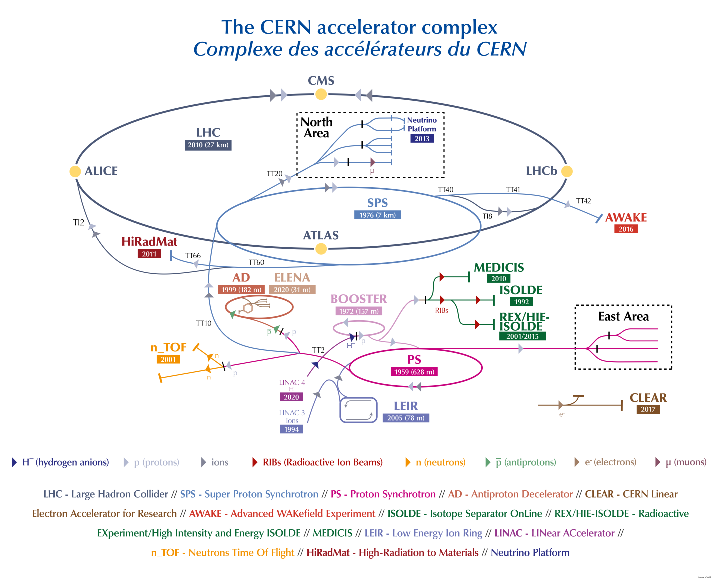
\includegraphics[width=\textwidth]{images/2-LHC-ATLAS/accelerator_complex.pdf}
\caption{An overview of the CERN accelerator complex \cite{CERN:2012:accelerators}. The \ac{LHC} is fed by a series of accelerators starting with Linac4. Next are the Proton Synchrotron Booster, the Proton Synchrotron, and finally the Super Proton Synchrotron which injects protons into the \ac{LHC}.}
\label{fig: accelerator-complex}
\end{figure}



%-------------------------------------------
%	Chapter 2: ATLAS
%-------------------------------------------
\section{The ATLAS Experiment}
\label{atlas-section}

\subsection{The ATLAS Detector}
The ATLAS detector is one of two general-purpose detectors in operation at the \ac{LHC} \cite{PERF-2007-01}. The experiment aims to make Standard Model (SM) precision measurements and test Beyond Standard Model (BSM) theories. In total, the detector is a 44 m long cylinder with a diameter of 25 m and weighs over 7000 tonnes, shown in Figure \ref{fig: atlas-detector}. The detector’s geometry is cylindrical consisting of a central barrel and two end-caps to ensure forward physics coverage and hermeticity. The ATLAS detector comprises of specialised sub-detectors, orientated coaxially around the nominal interaction point at the centre of the detector. 

\begin{figure}[htb!]
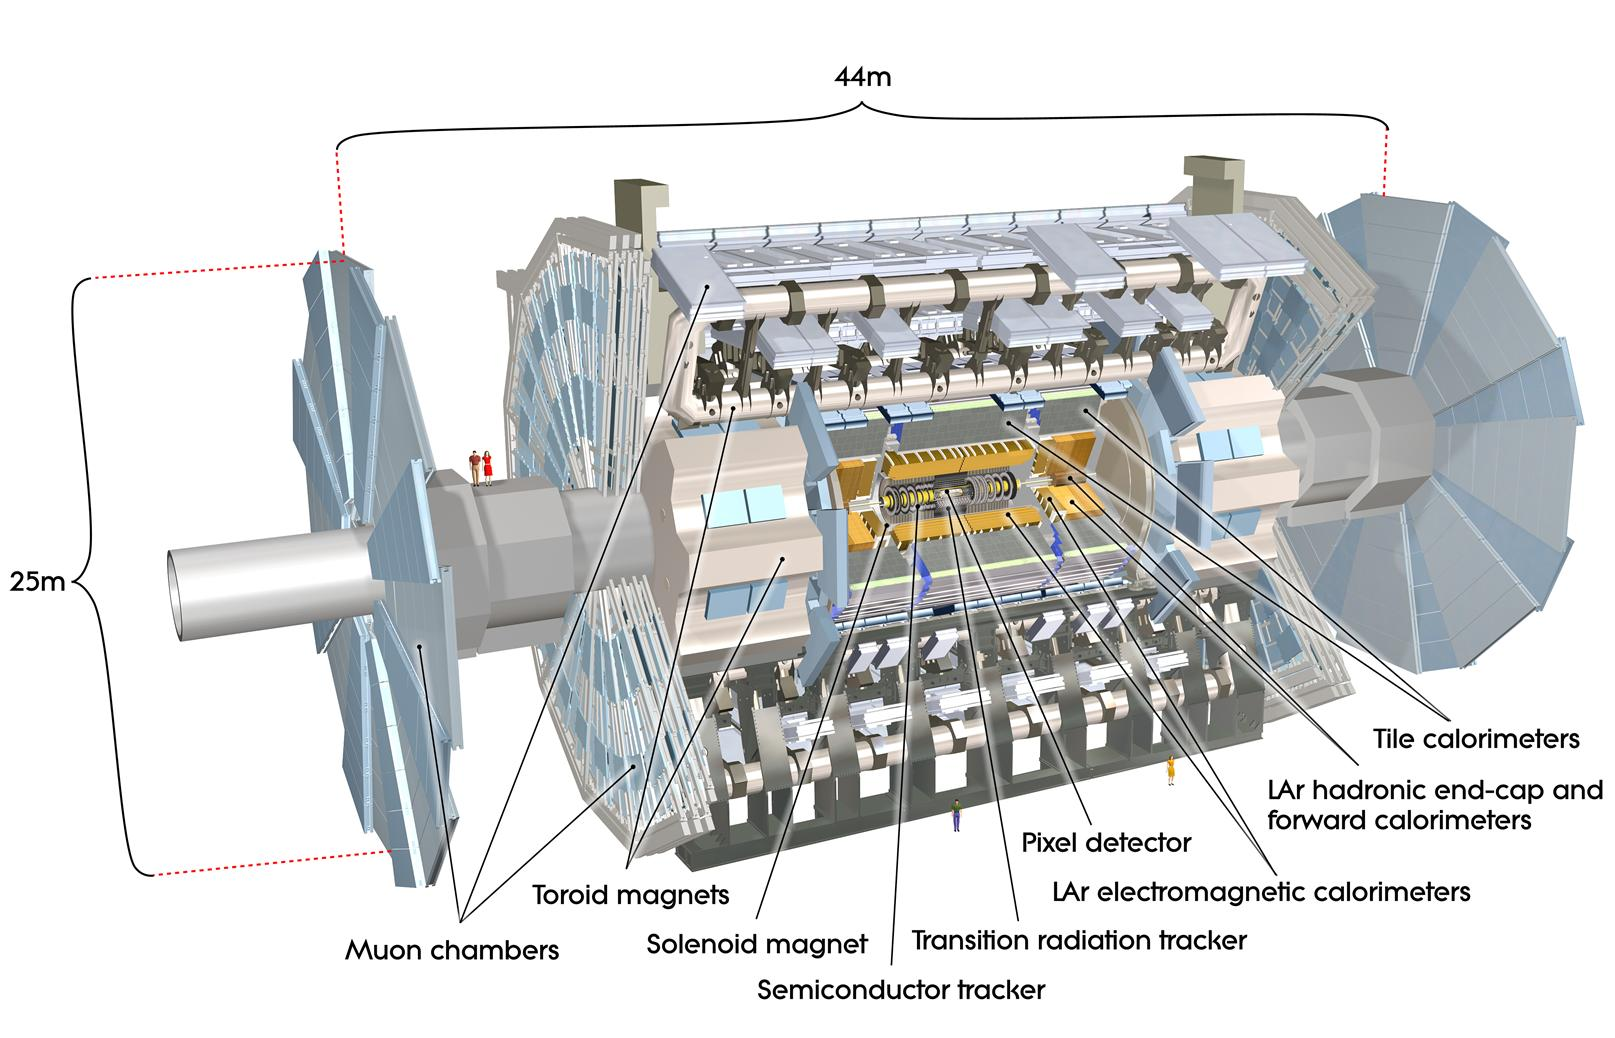
\includegraphics[width=\textwidth]{images/2-LHC-ATLAS/atlas_detector.jpg}
\caption{A 3D model of the entire ATLAS detector \cite{Jon-And:1237407}. Cutouts to the centre of the detector reveal the different sub-detectors which are arranged in concentric layers around the nominal interaction point.}
\label{fig: atlas-detector}
\end{figure}

In order of increasing radial distance, the ATLAS sub-detectors include the Inner Detector (ID) described in Section \ref{inner-detector}, the electromagnetic and hadronic calorimeters, and the outermost muon spectrometer. 

More comprehensive descriptions of the calorimeters and muon spectrometer can be found in the Technical Design Report for the ATLAS detector \cite{inner-detector-TDR}. Since the work in this thesis pertains to tracking, particular attention is given to the Inner Detector (ID) which houses the tracking systems of the ATLAS detector. In Section \ref{coordinate-system}, the coordinate system used at ATLAS and definitions for frequently occurring quantities are also provided.



%-------------------------------------------
%	Chapter 2: Coordinate system
%-------------------------------------------
\subsection{Coordinate System and Collider Definitions}
\label{coordinate-system}

%% based on https://twiki.cern.ch/twiki/bin/view/AtlasProtected/PubComCommonText

\subsubsection{The ATLAS Coordinate System}

The origin of the coordinate system used by ATLAS is the nominal interaction point in the centre of the detector. As shown in Figure \ref{fig:atlas-coord-system}, the z-axis points along the direction of the beam pipe, while the x-axis points from the interaction point to the centre of the \ac{LHC} ring, and the y-axis points upwards.
The transverse plane lies in $x$-$y$ while the longitudinal direction lies along the z-axis. A cylindrical coordinate system with coordinates ($r$,$\phi$) is used in the transverse plane, where $r$ is the radius from the origin and $\phi$ is the azimuthal angle around the z-axis.

\begin{figure}[!htbp]
  \centering
  % Author: Izaak Neutelings (June 2017)
% taken from https://tex.stackexchange.com/questions/159445/draw-in-cylindrical-and-spherical-coordinates
% Licensed under CC Attribution-Share Alike 4.0 International  https://creativecommons.org/licenses/by-sa/4.0/
% Original source https://wiki.physik.uzh.ch/cms/latex:example_spherical_coordinates
% Modifications by Giles Strong (March 2020):
% 1. Removal of some header code
% 2. Changing theta to eta
% 3. Addition of mountains
% 4. Changed "\draw[dashed,red] (O)  -- (Pxy);" to "\draw[->] (O)  -- (Pxy) node[right] {$p_t$};"
% Modifications by Giles Strong (April 2020):
% 1. Removal of Jura mountains
% 2. Rotated to be in terms of ATLAS coordinate system
% 3. Resized labels for the detectors

\tikzset{>=latex} % for LaTeX arrow head

\tdplotsetmaincoords{76}{45} % to reset previous setting 75 50
    \begin{tikzpicture}[scale=4.8,tdplot_main_coords,rotate around x=90]
    
    % variables
    \def\rvec{1.2}
    \def\thetavec{40}
    \def\phivec{70}
    \def\R{1.1}
    \def\w{0.3}
    
    % axes
    \coordinate (O) at (0,0,0);
    \draw[thick,->] (0,0,0) -- (1,0,0) node[below left]{$x$};
    \draw[thick,->] (0,0,0) -- (0,1,0) node[below right]{$y$};
    \draw[thick,->] (0,0,0) -- (0,0,1) node[below right]{$z$};
    \tdplotsetcoord{P}{\rvec}{\thetavec}{\phivec}
    
    % vectors
    \draw[->,red] (O) -- (P) node[above left] {$\vec{p}$};
    \draw[->] (O)  -- (Pxy) node[right] {$p_T$};
    \draw[dashed,red] (P)  -- (Pxy);
    \draw[dashed,red] (Py) -- (Pxy);
    
    % circle - LHC
    \tdplotdrawarc[thick,rotate around x=90,black!70!blue]{(\R,0,0)}{\R}{0}{360}{}{}
    
    % compass - the line between CMS and ATLAS has a ~12° declination (http://googlecompass.com)
    %\begin{scope}[shift={(1.1*\R,0,1.65*\R)},rotate around y=12]
    %    \draw[<->,black!50] (-\w,0,0) -- (\w,0,0);
    %    \draw[<->,black!50] (0,0,-\w) -- (0,0,\w);
    %    \node[below right,black!50,scale=0.6] at (\w,0,0) {N};
    %\end{scope}
    
    % nodes
    \node[right] at (\R,0,0) {LHC};
    \fill[radius=0.8pt,black!20!red]
        (O) circle node[left=4pt,below=5pt] {ATLAS};
    \draw[thick] (0.02,0,0) -- (0.5,0,0); % partially overdraw x-axis and CMS point
    \fill[radius=0.8pt,black!20!blue]
        (2*\R,0,0) circle
        node[right=4pt,below=2pt,scale=0.7] {CMS};
    \fill[radius=0.8pt,black!10!orange]
        ({-\R*sqrt(2)/2+\R},0,{-\R*sqrt(2)/2}) circle % 45 degrees from ATLAS
        node[left=2pt,below=2pt,scale=0.7] {ALICE};
    \fill[radius=0.8pt,black!60!green]
        ({-\R*sqrt(2)/2+\R},0,{\R*sqrt(2)/2}) circle % 45 degrees from ATLAS
        node[below=6pt,right=3pt,scale=0.7,anchor=north east] {LHCb};
    
    % arcs
    \tdplotdrawarc[->]{(O)}{0.2}{0}{\phivec}
        {above=2pt,right=-1pt,anchor=mid west}{$\phi$}
    \tdplotdrawarc[->,rotate around z=\phivec-90,rotate around y=-90]{(0,0,0)}{0.5}{0}{\thetavec}
        {anchor=mid east}{$\eta$}
\end{tikzpicture}
  \caption{
    The coordinate system used at the ATLAS detector, showing the locations of the four main experiments located at various points around the \ac{LHC}. The 3-vector momentum $p_{\text{T}} = (p_x, p_y, p_z)$ is shown by the red arrow. Reproduced from \cite{Strong:2020mge}.
  }
  \label{fig:atlas-coord-system}
\end{figure}

Additionally, the transverse $x$-$y$ plane is often used to describe the kinematics of collisions, where the transverse momentum $p_{\text{T}}$ of an object is the projection of its momentum on the transverse plane, given by Eq \ref{eq:pt}.

%
\begin{equation}\label{eq:pt}
  p_\text{T} = \sqrt{ {p_x}^2 + {p_y}^2 }
\end{equation}



%The pseudorapidity is defined in terms of the polar angle $\theta$ as $\eta = -\ln \tan(\theta/2)$.


\subsubsection{Pseudorapidity}

The pseudorapidity, $\eta$, is a commonly used spatial coordinate describing the polar angle, $\theta$, of a particle's trajectory relative to the beam axis, and is defined as:
%
\begin{equation}\label{eq:pseudorap}
  \eta = - \ln \left[ \tan \left( \frac{\theta}{2} \right) \right] .
\end{equation}
%
The pseudorapidity is a convenient quantity to work with as differences in $\eta$ are invariant under Lorentz boosts. In addition, particle production is constant as a function of $\eta$.


%-------------------------------------------
%	Chapter 2: The Inner Detector
%-------------------------------------------
\subsection{The Inner Detector}
\label{inner-detector}

The ID system provides high-resolution charged particle trajectory tracking in the range $ \lvert \eta \rvert < 2.5$. The ID is immersed in a 2 T axial magnetic field, produced by a superconducting solenoid magnet, which enables the measurement of particle momentum and charge. The ID is made up of several sub-systems shown in Figures \ref{fig:atlas-id-run1} and \ref{fig:atlas-id-run2}. Each sub-system contains specialised hardware and contributes towards a full track reconstruction. 

\begin{figure}[!htbp]
  \centering
  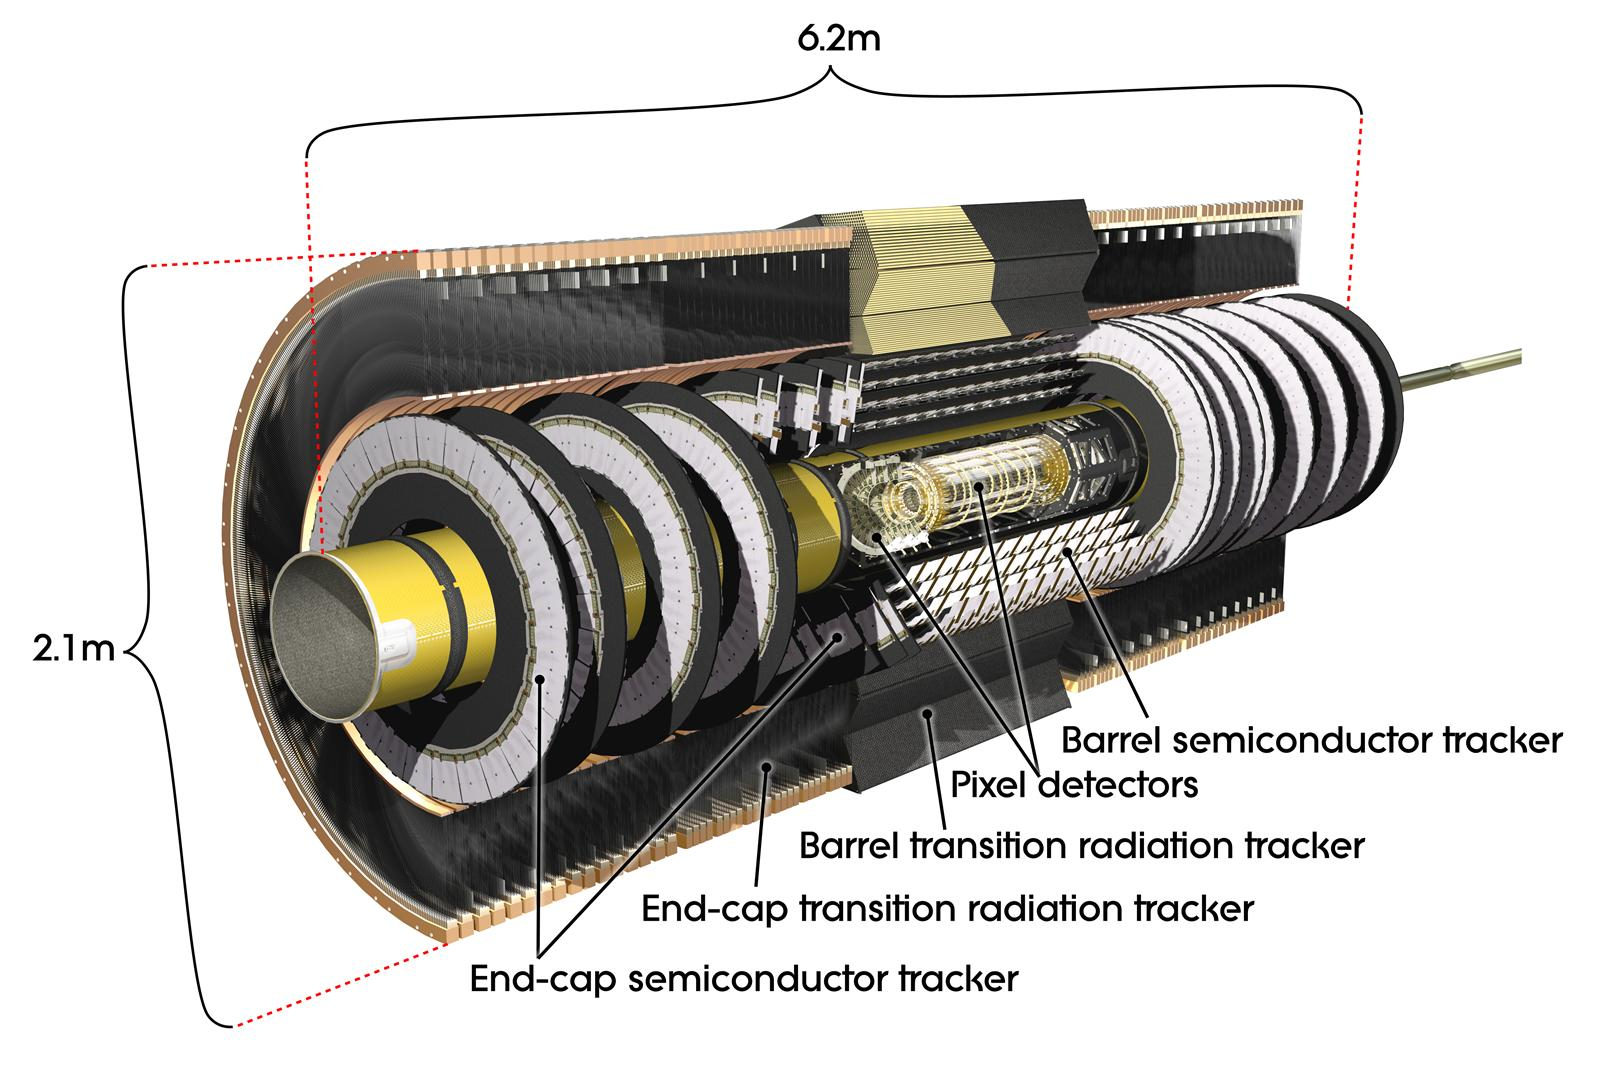
\includegraphics[width=0.85\textwidth]{images/2-LHC-ATLAS/atlas_id.jpg}
  \caption{
    A 3D model of the ATLAS ID, made up of the pixel and semi-conductor tracker sub-detectors, showing the barrel layers and end-cap disks \cite{atlasid}.
  }
  \label{fig:atlas-id-run1}
\end{figure}

\begin{figure}[!htbp]
  \centering
  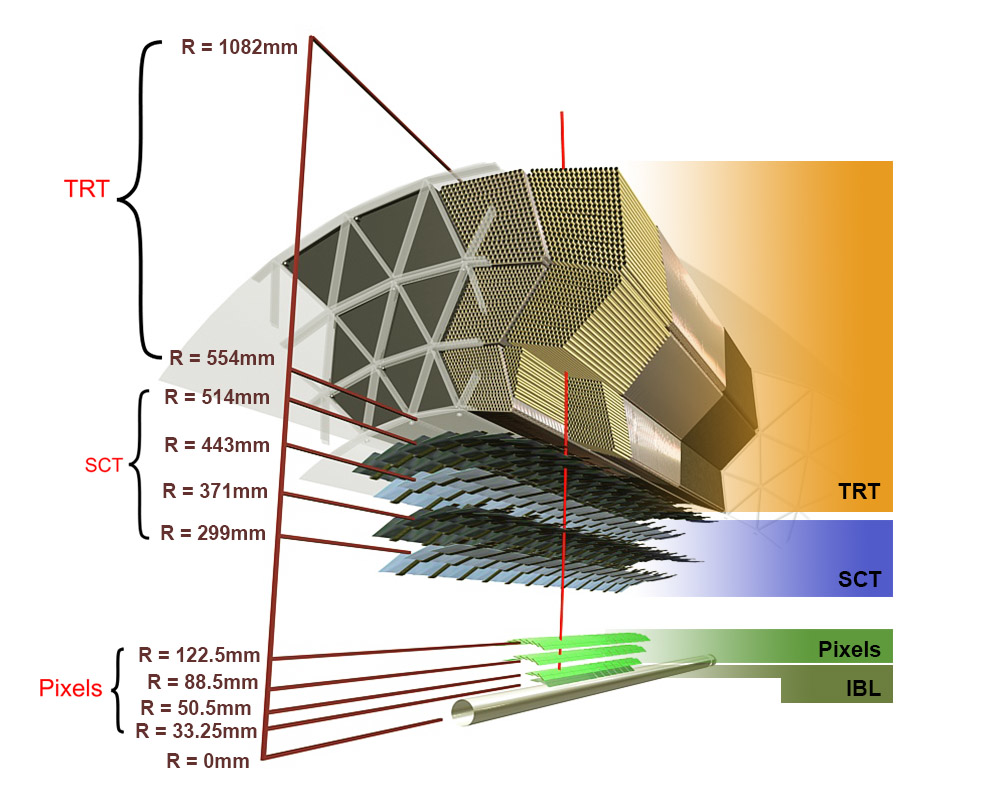
\includegraphics[width=0.85\textwidth]{images/2-LHC-ATLAS/atlas_id_xs.png}
  \caption{
    A cross-sectional view of the ATLAS ID, with the radii of the different barrel layers shown \cite{atlastrackingdocs}.
  }
  \label{fig:atlas-id-run2}
\end{figure}

\subsubsection{Pixel Detector}

The innermost silicon pixel detector \cite{pixel} provides high-granularity measurements covering the interaction region and typically provides four space-point measurements per track. The silicon pixel detector comprises four cylindrical barrels at increasing radii from the beamline, and four end-cap disks on each side. The innermost barrel layer is the Insertable B-layer (IBL), which was installed before Run 2 \cite{ATLAS-TDR-19,PIX-2018-001} and lies approximately just 33 mm from the beam axis. The second-to-innermost layer is often referred to as the B-layer. The pixel detector was initially constructed with 80 million readout channels, with the IBL providing an additional 12 million \cite{ibl}. The specification of the pixel detector determines the impact parameter resolution and the ability to reconstruct primary and secondary vertices. Individual pixels are 50 $\mu$m in the transverse direction (see Section \ref{coordinate-system} for the ATLAS coordinate system) and 400 $\mu$m in the longitudinal $z$ direction (250 $\mu$m for the IBL). Cluster positions have a resolution of approximately 10 $\mu$m in $(r,\phi)$ and 100 $\mu$m in $z$.


\subsubsection{Semi-Conductor Tracker (SCT)}

The pixel detector is followed by the SCT, which is made up of four concentric barrel layers in the central region, and nine disks in each end-cap. Each layer is itself made of a pair of silicon microstrip layers, with a small stereo angle (40 mrad) between the two layers enabling the $z$-coordinate to be measured from a pair of strip measurements. The operation of the silicon sensors is based on the properties of the p-n junction \cite{6773080}. At the junction between the p-type doped silicon and the n-type doped silicon the electrons (holes) diffuse from the n-type (p-type) side and recombine with holes (electrons) on the p-type (n-type) side. The diffusion of the electrons (holes) leaves behind ionised donor (acceptor) atoms and an electric field develops across the junction which inhibits further diffusion until equilibrium is reached. The space charge region formed around the junction is now devoid of mobile charge carriers and is referred to as the depletion region. Applying an external reverse bias voltage to the p-n junction draws electrons (holes) away from the n-type (p-type) side and increases both the depletion region width and the electric field across the junction. Ionising particles traversing the sensor create electron-hole pairs in the depletion region, which are swept to the electrodes by the electric field and induce an electrical current in the external circuitry. In silicon microstrip sensors, like those in the SCT, one (or both) of the electrodes are segmented in order to provide position measurements. The SCT typically provides a further four space-point measurements (eight strip measurements, or hits) per track in the barrel region. See Ref. \cite{inner-detector-TDR} for further information.


\subsubsection{Transition Radiation Tracker (TRT)}

The TRT is a straw-tube tracker which complements the higher-resolution silicon- based tracks by offering a larger number of hits per track and a long lever arm. This aids the accurate measurement of particle momentum and enables radially extended track reconstruction up to $ \lvert \eta \rvert = 2.0$. It is made up of approximately 300,000 drift tubes with a diameter of 4 mm which are filled with an argon/xenon gas mixture. The walls of each tube are electrically charged, and a thin conducting wire runs along the center. When a charged particle traverses a tube, it ionises the gas and the resulting liberated electrons drift along the electric field to the wire, where an associated charge is registered. In the barrel the straws run parallel to the z-axis and therefore the TRT only provides tracking information in $(r, \phi)$. Straws are arranged radially in the end-caps. The resulting two-dimensional space-points have a resolution of approximately 120 $\mu$m. The spaces between the straws are filled with a polymer which encourages the emission of transition radiation, aiding electron identification.

\subsubsection{The Inner Tracker (ITk) Upgrade}

The current ID has various limitations that hinder its performance as the \ac{LHC} machine is upgraded. Radiation damage and high detector occupancy result in the requirement for a full replacement of the ID after Run-3 with the new ITk \cite{pileup,itk-strip}. One significant change in the detector layout is that the ITk will consist only of high granularity silicon detectors, replacing the TRT. This will extend to a 1 m radius, whereas the current SCT outer layer extends only to 60 cm. The acceptance of the detector will be increased such that that the strip detector covers a range of $ \lvert \eta \rvert = 2.7$ with the pixel detector extending the range to $ \lvert \eta \rvert = 4.0$. The improved radiation hardness is designed to cope with greater fluence values in the harsh conditions expected at the HL-LHC. In addition, the ITk material is designed to minimize the effects of multiple scattering and energy losses before particles reach the outer detector components.

%Outside of the pixel detector, the SCT measures charged particles at an intermediate distance from the collision point and improves the determination of vertex position and track momentum. The SCT consists of four barrel layers and nine end-cap layers on each side. The outermost section of the ID, the TRT, is used for the identification of charged particles and consists of drift tubes that are filled with a mixture of Xe, CO2 and O2, and contain a central gold-plated tungsten wire. When charged particles traverse the TRT, the gas inside the straws is ionised and the free electrons drift towards the wire and are amplified and then read out. In addition, transition radiation provides information on the particle type that passed through the tracker.





%-------------------------------------------
%	Chapter 2: TDAQ
%-------------------------------------------
\subsection{The Trigger}
The 25 ns bunch spacing used over the course of Run 2 corresponds to a bunch-crossing or event rate of 40 MHz (see Table \ref{tab:lhc-runs}). If the full information for the detector was written out for each event, this would correspond to the generation of 60 TB of data each second. This is more than feasibly possible for the read out from the hardware, the processing and storage of the data. This requires the use of a trigger system which quickly makes a decision about whether or not an event is potentially interesting and should be kept for further analysis. The trigger system comprises two levels which search for signs of electrons, muons, taus, photons and jets, as well as events with large total or missing transverse energy. The hardware-based Level-1 (L1) trigger uses coarse information from the calorimeters and muon spectrometer to accept events at an average rate of 100 kHz approximately 2.5 $\mu$s after the event. After the L1 trigger, the software-based High Level Trigger (HLT) makes use of 40,000 CPU cores to make a final selection on surviving events, using full granularity detector information in approximately 200 ms. The final event read-out rate is approximately 1.2 kHz, corresponding to 1.2 GBs$^{-1}$ of permanent data storage. More information is provided in \cite{TRIG-2016-01}.


%-------------------------------------------
%	Chapter 2: Inner Detector Trigger
%-------------------------------------------
\subsubsection{The Inner Detector Trigger}

The ability of the ATLAS trigger system to process information from the ID to reconstruct particle trajectories is an essential requirement for the efficient triggering of physics objects. The ID trigger must therefore be able to reconstruct tracks with high efficiency across the entire range of possible physics signatures, as well as handle the input rate of the HLT. This challenge is exacerbated by the very high track and hit multiplicities in the ID that arise from the large pile-up. 

The ID trigger is designed to perform fast online track and vertex reconstruction using measurements from the ID. For Run 2, the ID trigger tracking is performed in two steps; the first algorithm handles trigger-specific pattern recognition and seeded track finding to generate medium quality tracks as quickly as possible. This is collectively known as the \textit{Fast Track Finder} (FTF) algorithm \cite{Penc:2104217, Grandi:2624768}. This step is followed by the \textit{Precision Tracking} (PT), which relies heavily on offline tracking algorithms \cite{T_Cornelissen_2008} improving the track purity and quality by applying tighter requirements. 



%-------------------------------------------
%	Chapter 2: Motivation for Hi-Lumi LHC
%-------------------------------------------
\section{Motivation for the HL-LHC}
\label{hi-lumi}

% - the physics motivation to increase the luminosity - brief 

The HL-LHC is an upgrade of the \ac{LHC} to extend its physics reach, particularly in terms of precision measurements in the Higgs sector, by increasing the data collected by an order of magnitude. This will be achieved by increasing the LHC instantaneous luminosity by a factor of up to five compared to the nominal. This will enable the detector's discovery potential and exploration potential to significantly improve. Initially, the luminosity will be increased to $5 \times 10^{34}  \text{ cm}^{−2}\text{s}^{−1}$, and subsequently up to $7.5 \times 10^{34}  \text{ cm}^{−2}\text{s}^{−1}$ by the mid-2030s.

Since the discovery of the Higgs boson at the ATLAS and CMS experiments \cite{ATLAS-HIGGS, CMS-HIGGS} in 2012, the study of the Higgs sector has greatly expanded to include many precision measurement analyses, predictions from theory and searches for rare production and decay processes. One important question to answer is whether the observed Higgs boson is that predicted from the SM electroweak symmetry breaking mechanism \cite{ewsb} or if it is, in fact, the first signal in some BSM physics. With the accumulated data so far, the identity of the Higgs boson is consistent with SM predictions, but higher-precision measurements could illuminate any potential discrepancies from prediction. Further information on the Higgs mechanism can be found in \cite{Bednyakov_2008}.

%With the accumulated data so far, the identity of the Higgs boson is consistent with SM predictions and all measurements are confined to the couplings of the Higgs to SM particles, which are proportional to the particles’ masses, but higher-precision measurements of these couplings could illuminate any potential discrepancies from prediction.

In general, precision measurements of the Higgs sector provide indirect probes to just about any extension of the Standard Model. There are many theoretical particles predicted by various BSM scenarios that can also be searched for in the HL-LHC. One set of such scenarios falls under the title of Super-Symmetry \cite{supersym}, which predicts super-partners belonging to every fermion and every boson. Direct dark matter searches can also be probed at higher mass scales, and new detector upgrades will facilitate searches for long-lived exotic particles. Additionally, BSM physics can be further probed through rare \textit{b} and \textit{c} hadron decays that may be measured using the increased integrated luminosity \cite{wg-bsm}.

The physics programme offered by the HL-LHC is vast \cite{big-report}; a detailed description of the project and its technological and operational challenges is provided in the HL-LHC Preliminary Design Report \cite{Apollinari:2116337}. The programme would deliver a significant potential for new physics discoveries and incredibly high-precision SM measurements. However, the promising plan for the future is accompanied by many technical challenges that each of the experiments face. The increased luminosity results in greater pile-up, which results in drastically higher detector occupancy and radiation levels. In the case of ATLAS, Figure \ref{fig:pileup-walltime} shows the projected evolution of compute usage from 2020 until 2036 under different R\&D scenarios. The expected pile-up levels during the HL-LHC are around $\langle \mu \rangle$ = 200, demonstrating the need for upgrades to both the detector and algorithmic designs.

\begin{figure}[!htbp]
  \centering
  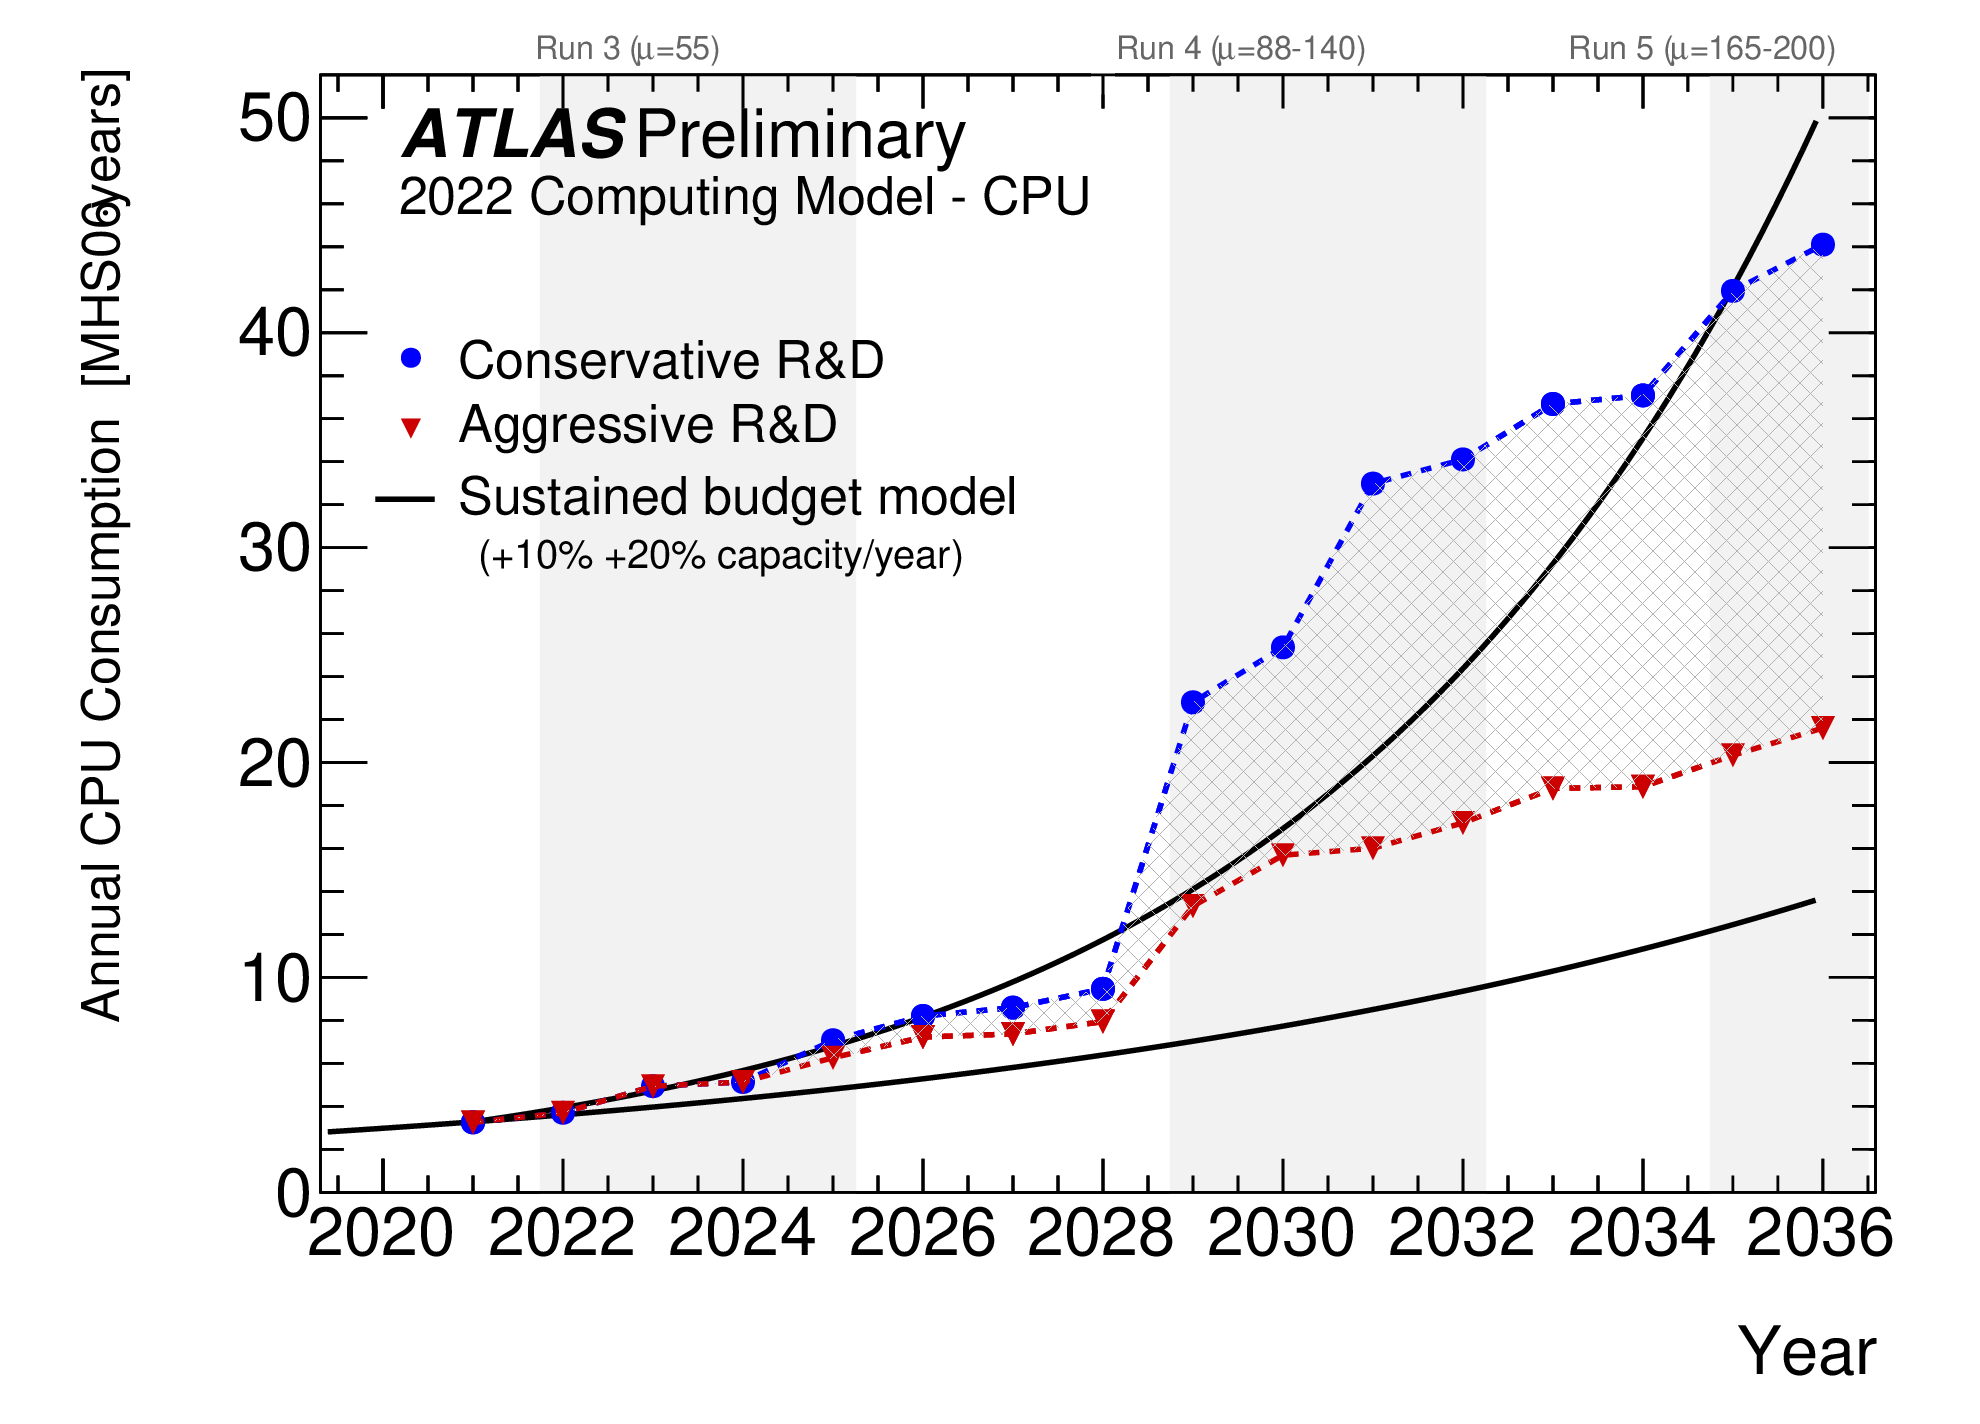
\includegraphics[width=0.8\textwidth]{images/2-LHC-ATLAS/computing-model.png}
  \caption{
    Projected evolution of compute usage under the conservative (blue) and aggressive (red) R\&D scenarios. The darker shading between the red and blue lines illustrates the range of resource consumption if the aggressive scenario is only partially achieved. The black lines indicate the impact of sustained year-on-year budget increases and improvements in new hardware, that together amount to a capacity increase of 10\% (lower line) and 20\% (upper line). The vertical shaded bands indicate periods during which ATLAS will be taking data \cite{Collaboration:2802918}.
  }
  \label{fig:pileup-walltime}
\end{figure}

%In the case of ATLAS, Figure \ref{fig:pileup-walltime} shows how the reconstruction time per event increases with pile-up. The increase in time is exponential, and the expected pile-up levels during the HL-LHC are around $\langle \mu \rangle$ = 200, demonstrating the need for upgrades to both the detector and algorithmic designs in ATLAS.

%\begin{figure}[!htbp]
%  \centering
%  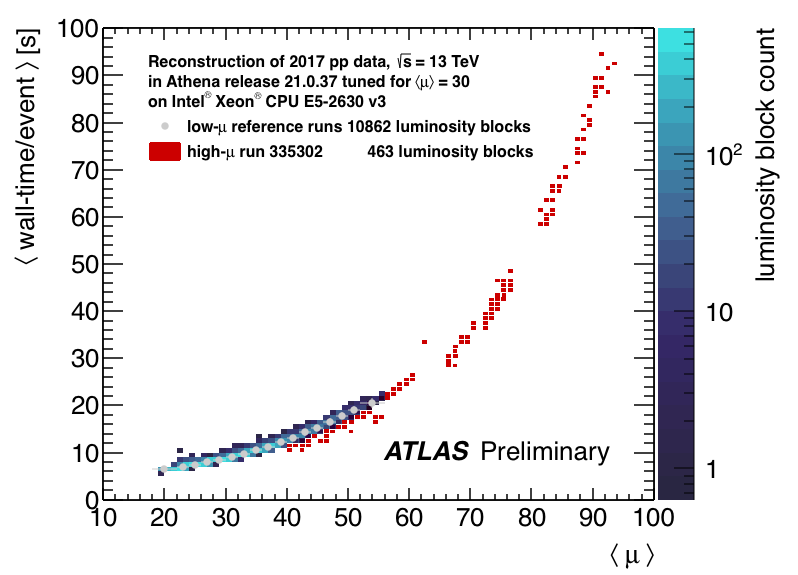
\includegraphics[width=0.8\textwidth]{images/2-LHC-ATLAS/pileup-walltime.png}
%  \caption{
%    The dependency of reconstruction wall time per event on pileup. The luminosity block count represents short intervals of data taking, in which the instantaneous luminosity is estimated, and from this the integrated luminosity derived \cite{pileup}.
%  }
%  \label{fig:pileup-walltime}
%\end{figure}

\doublespacing

%-------------------------------------------
%	Chapter 3: Track Reconstruction
%-------------------------------------------
\chapter{Track Reconstruction}
\label{chapter-3}

%H important to help show the bigger picture of my research and the motivation behind the work presented

%Successful particles physics measurements are dependent on an efficient and performant re- construction of the physics objects from the detector measurements. As a community we are always striving to run at the edge of the available detector and computation capabilities to ex- tract the maximum amount of information from the experiments. Tracking detectors are at the core of most collider experiments and track reconstruction is one of the crucial tasks in every reconstruction chain.

%Track reconstruction at its heart is a combinatorial problem, i.e. to find the measurements that originate from the same initial particle from a set of possible combinations. The created particles have a wide range of possible properties, especially different creation vertices and momenta, and their particle trajectories have non-deterministic contributions from material interactions. In combination with inhomogeneous magnetic fields and detector inefficiencies, this leads to the possibility of confusion, fake tracks, etc. . All of these effects depend strongly on the density of the measurements and thus on the collision pile-up. Consequently, with the upcoming upgrade to the High-Luminosity Large Hadron Collider (HL-LHC) the track reconstruction complexity will increase significantly.

In this chapter, track finding in silicon based detectors is presented. Section \ref{track-finding-silicon-trackers} outlines a typical workflow for track reconstruction in a multi-element silicon tracker and the parameterisation used for specifying the trajectory of charged particle tracks. Section \ref{ml-background} presents the theoretical formalism of a typical ML classification problem, as well as an introduction to the TrackML detector and its corresponding ML challenge. This section focuses on the realistic detector geometry used to simulate measured particle hits similar to those expected of the HL-LHC experiment, as well as the approaches and ideas to tackle the challenge of track reconstruction that arose from the challenge. Finally, graph network architectures and track reconstruction using graph networks is presented in Section \ref{graph-networks}, as a potential solution and optimisation to the track finding problem.


%The aim of this project is to explore track finding methods utilizing a graph-based track model and graph neural networks (GNN). An ML-based algorithm will be used to predict a graph adjacency matrix given the input hit features such as a shape of a charge cluster representing a track position measurement in a silicon detector. The excitation/inhibition rules of individual GNN neurons will be designed to facilitate the “simple-to-complex” approach for “hits-to-tracks” association such that the network starts with relatively “easy” areas of an event with low hit density and gradually progresses towards more complex “hot” areas. To efficiently exploit a priori knowledge about charged particle dynamics the GNN-based algorithm will be using simplified Kalman filters as mechanisms for information propagation and track extraction. 

% first talk about graph building using the ML hit pair predictor and then talk about graph pruning/track extraction using the GNN based algorithm



%--------------------------------------------------
%	Chapter 3: Track finding in Silicon Trackers
%---------------------------------------------------
\section{Track Finding in Silicon Trackers}
\label{track-finding-silicon-trackers}

%The reconstructed trajectories of charged particles are referred to as tracks. 
%Tracks are reconstructed from the energy depositions (called hits) left by the particles as they traverse the the inner detector.


Tracks are reconstructed from the energy depositions (\textit{hits}) left by the particles as they traverse the inner detector. Tracks are used in the reconstruction of other objects, including vertices and jets, so their accurate reconstruction is a critical task. A typical workflow for track finding in a multi-element silicon tracker (such as those in ATLAS and CMS) is given below and comprises a three-stage approach; seeding, track following, and track selection, implemented in many charged particle tracking algorithms and is commonly known as the \textit{inside-out} approach. A comprehensive introduction to ATLAS tracking is available in Ref \cite{Cornelissen:2007vba}.

%The main sequence is referred to as ’inside-out’ track finding, involving clusterisation [17], a CPU-expensive ’track-finding’, followed by precise estimation of track parameters via ’track-fitting’.


%--------------------------------------------------
%	Chapter 3: Track Reconstruction
%---------------------------------------------------
\subsection{Inside-Out Track Reconstruction}
\label{track-reconstruction}

%Describe a typical workflow for track finding in a typical multi-element silicon tracker such as ATLAS and CMS. This workflow is basically a three-stage approach with the seeding, track following, and track selection implemented in the current charged particle tracking algorithms. This is precisely the right place to introduce the TrackML setup. Add that the high-lumi LHC motivates the R\&D of new track finding techniques and we need an environment for fast prototyping and testing various techniques which would allow expert from outside HEP to contribute hence the TrackML.

%This section should be all about track finding in ATLAS, including the main pipeline outlining space-point formation (clustering), track finding (combinatorics), ambiguity solving, neural network cluster splitting, pattern recognition techniques, Kalman filters etc 


\subsubsection{Space-point Formation (Clustering)}
When a charged particle traverses a silicon layer, charge can be deposited in more than one pixel or strip. This is due to the incident angle of the particles with respect to the sensor and also the drift of electrons inside the sensor caused by their interaction with the magnetic field. Clusters are formed by grouping together neighbouring pixels or strips. The local position of the cluster on the sensor is typically estimated using the energy-weighted mean position of the pixels (or strips) forming the cluster. The clusters are then converted into 3D space-points by a coordinate transformation, where pixel space-points are identical to pixel clusters and strip space-points are formed by combining information from two strip clusters in subsequent sensors in the SCT (or strip double layers of the ITk).

\subsubsection{Seeded Track Finding}
Space-points are used to build track seeds. Seeds are defined as a group of three space-points located in different detector layers which are geometrically compatible with being part of a track segment. A combinatorial KF is used to build track candidates by extending track seeds. The filter searches for adjacent clusters both outwards and inwards in $r$ while attempting to smooth the trajectory. This method considers tracks as a sequence of hits and, from a particular starting point, will attempt to extrapolate throughout the detector collecting hits belonging to the same track. The filter can create multiple track candidates per seed, with bifurcations along the track occurring when more than one compatible space-point exists in a given detector layer. In this way, the filter creates an excess of track candidates, which are only required to satisfy basic quality requirements. Track candidates are allowed to share hits freely (a single hit may be used by multiple track candidates). Typically, the presence of shared hits is an indication of a bad track due to the high granularity of the ATLAS tracking detectors. At this stage, there can also be a large number of incorrect hits assigned to otherwise good tracks, and large numbers of fake tracks. Fake tracks are those where the majority of associated hits do not originate from the trajectory of any one physical particle. The end result of this track finding/pattern recognition process is a set of potential track candidates, generally of low quality, that then undergoes further refinement through an ambiguity resolution step in which the highest quality tracks are selected. The implementation of the filter approach in tracking is fast computationally, but is relatively imprecise and does not resolve ambiguities.

\subsubsection{Track Ambiguity Resolution}
\label{chapter-3-ambiguity-resolution}

The procedure so far has created candidates with potential overlap. In the ambiguity solver of the ATLAS detector, track candidates are processed individually in descending order of a track score in an effort to resolve this overlap. The track score quantifies the likelihood of the track corresponding to the trajectory of a real particle. Scoring uses a number of variables, including the number and positions of hits, the transverse momentum of the track and the fit quality described as the $\chi^{2}$ divided by the number degrees of freedom on the track. A preference for high transverse momentum tracks promotes the successful reconstruction of the more physically interesting energetic particles, and suppresses the large number of wrong hits assigned to low momentum tracks. The refined and purified track candidates resulting from the ambiguity resolution are re-fit using a global $\chi^{2}$ method in order to obtain the high-precision track parameter estimate. This accounts for errors on the measurements and expected uncertainties (e.g multiple scattering etc.) Ambiguity solving was introduced as part of the ATLAS New Tracking (NEWT) \cite{Cornelissen:2007vba} intended to improve track reconstruction performance in dense environments. 

\subsubsection{TRT Extension}
The successful tracks from the ambiguity solving stage are extended into the TRT. The TRT operates as a drift chamber: when a charged particle traverses a straw, the active gas mixture is ionised creating ionisation clusters.  The clusters are collected by applying a large potential difference between the wall of the straw and the wire. By measuring the time it takes the clusters to reach the wire, the distance of the track to the wire can be determined, and a valid set of matching drift circles can be formed. A road is then formed along the extrapolated track and the TRT drift circles that fall within this road are collected. Left/right ambiguities for the TRT drift circles are resolved and the output consists of the original tracks together with a list of associated TRT drift circles. A subsequent track refit is performed using the global $\chi^{2}$ fitter \cite{TGCornelissen2008}, in order to increase the precision in parameters of the reconstructed track. Unlike the KF, the global $\chi^{2}$ fitter is beneficial in its application in the TRT as it looks at all measurements at the same time and iteratively minimises the starting parameters. This differs from the KF, which determines the track state vector dynamically from measurements at each detector surface and requires a starting surface to proceed in its filtering. 

%In addition, the xenon gas in the straws is sensitive to transition radiation photons that are produced in the radiator material between the straws. As electrons produce many more photons than other particles through Bremsstrahlung, this difference is used in electron identification. 



% need to discuss this section in more detail, talk about the drift circles, bremstrahlung, using the global chi-2 fit to increase the resolution of pT and ....another parameter. how is the TRT included into the track fit. a global chi-2 refit is done, doesn't use the kalman filter, why? - motivate the chi2 fit


\subsection{The Outside-In Sequence}
The inside-out sequence of the ID, described in the aforementioned section, relies on a track seed to be found in the silicon detector. Although being very efficient, not all tracks can be found through an inside-out procedure: ambiguous hits can shadow the track seed in the silicon and prevent the score of the silicon seeded track to survive the ambiguity processor. In addition to this, tracks coming from secondary decay vertices further inside the ID volume or from photon conversions may not have any silicon hits (or only an insufficient number) to comply with the inside-out sequence. Clearly, when no candidate track in the silicon detector is found, the extension into the TRT is automatically lost. A second, reverse sequence has therefore been deployed that starts a global pattern recognition in the TRT. Track segments are identified using a standard Hough transform mechanism, while a dedicated association tool prevents hits that have already been assigned to tracks in the inside-out procedure to be used again (which saves a significant amount of CPU time).



%--------------------------------------------------
%	Chapter 3: Track Parameterisation
%---------------------------------------------------
\subsection{Track Parameterisation}
\label{track-parameterisation}

Tracks must be parameterised in order to extrapolate them to outer detector layers, to include further hits. There are several parameterisations of tracks, but since the shape of charged particle trajectories in a uniform magnetic field is helical, in general five parameters are required to approximate the true trajectory. One such parameterisation is known as perigee given by Eq. \ref{perigee}:

\begin{equation}\label{perigee}
\textbf{p} = (d_0, z_0, \phi, \theta, Q/p_T)
\end{equation}

The respective transverse and longitudinal impact pararameters; $d_0$ and $z_0$ specify the distance of closest approach of the trajectory of a particle to the nominal interaction point. $\phi$ is the azimuthal angle in the $x$-$y$ plane and $\theta$ is the polar angle in the $(r,z)$ plane. In fact, we often use $\cot(\theta)$ instead of $\theta$, since $\cot(\theta)$ is the inverse slope of the track. $Q/p_T$ is the inverse transverse momentum multiplied by the charge of the particle. Figure \ref{fig:track-parameters-perigee} shows each of these parameters diagrammatically.


\begin{figure}[!htbp]
  \centering
  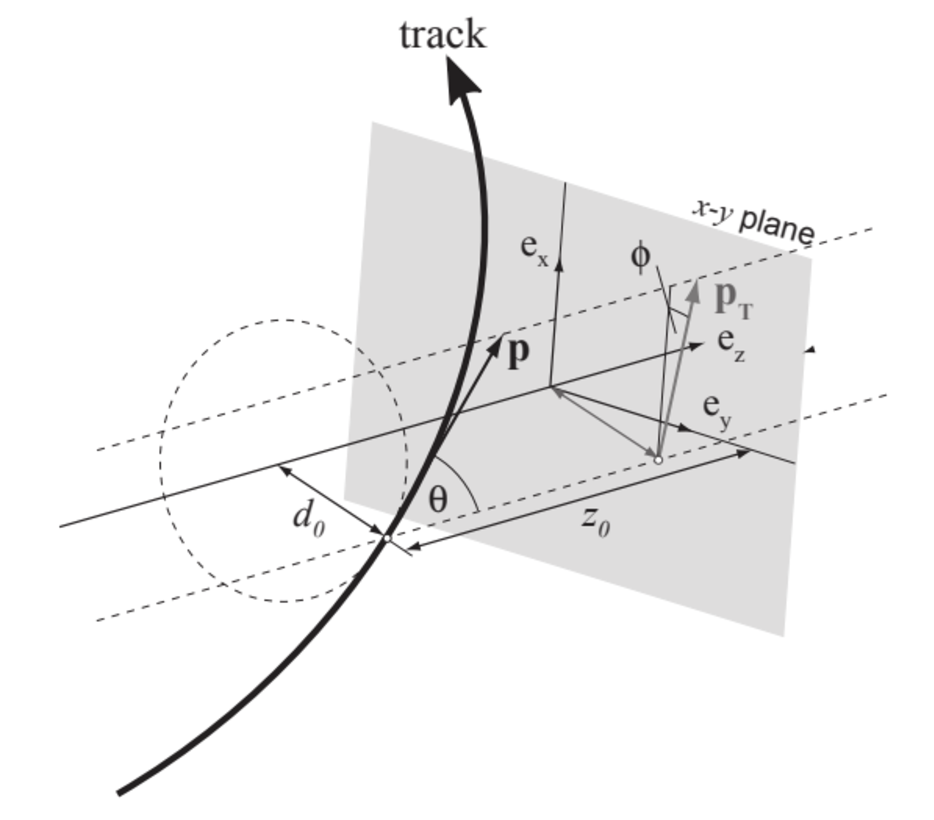
\includegraphics[width=0.65\textwidth]{images/3-track-reconstruction/track_params.pdf}
  \caption{Illustration of the perigee track parameters. Five coordinates are specified $(d_0, z_0, \phi, \theta, Q/p_T)$, defined at the track’s point of closest approach to the nominal interaction point at the origin of the coordinate system. The three-momentum \textbf{p}, transverse momentum $p_T$ and basis vectors $e_x$, $e_y$ and $e_z$ are also shown. Reproduced from Ref. \cite{atlastrackingdocs}
  }
  \label{fig:track-parameters-perigee}
\end{figure}






%--------------------------------------------------
%	Chapter 3: TrackML Model
%---------------------------------------------------
\section{Machine Learning in Track Reconstruction}
\label{ml-background}

\subsection{Machine Learning Background}

Over the past few decades, ML techniques have become increasingly prevalent in High Energy Physics experiments due the increased volumes of high-dimensional data and improvements in the field. Machine learning is the process by which a computer program uses data to learn suitable parameters for a predictive model. This is opposed to explicitly providing instructions on how to perform a task. A subfield known as \textit{supervised learning} is used in this work, and consists of exposing a model to a large number of labelled examples in order to extract relationships between the input data and their labels. These relationships are often complex, and explicitly programmed rules can fail to fully capture the relationships between inputs and outputs, as well as generalise to unseen data.

In the simplest case, a set of $n$ labelled training examples $S = \{(\textbf{x}_1, y_1), ..., (\textbf{x}_n, y_n)\}$ is collected. Each element $(\textbf{x}_i,y_i)$ consists of an input vector $\textbf{x}_i$ of dimension $m$, and the corresponding label $y_i$. In classification problems, typically $m$ is the number of unique features used to train the predictive model and the labels are integer class labels $y_i \in \{0,...,N − 1\}$, where $N$ is the number of categorical classes the training example belongs to (otherwise known as ground truth information). The rest of the discussion in this thesis is limited to binary classification problems ($N = 2$). Collecting sufficient and suitable data is one of the primary challenges of machine learning, as such data is not always readily available. Fortunately, sophisticated tools to simulate particle collisions have already been developed by the scientific community, one such example is in Ref \cite{Boos:2001cv}, as well as the others discussed further in Section \ref{trackml-simulation}. These tools play a key role in generating a suitably large amount of labelled data which is used to train algorithms.

After obtaining suitable training data, the next step is to define a model. Given an input domain of dimension $m$ and an output domain (0, 1), the model $f_{\theta} : \mathbb{R}^{m} \to (0, 1)$ is a parameterised functional mapping from input space to output space. Given an input example $\textbf{x}_i$ and a set of parameters $\theta$, the model outputs a prediction $\hat{y}_i \in (0, 1)$ for the true label $y_i$, as in:


\begin{equation}
    f_{\theta}(x_i) = \hat{y}_i
\end{equation}

The output $\hat{y}_i$ is in the interval (0, 1) so as to be interpreted as the probability that the input example $\textbf{x}_i$ belongs to class 1, commonly referred to as the $signal$ class. The parameters $\theta$ of the model are typically optimised and the model is designed to be expressive enough to correctly map the inputs $\textbf{x}_i$ to the outputs $y_i$. To perform this optimisation, the model is trained, which amounts to showing the model a series of labelled training examples and modifying the parameters of the model based on its ability to correctly predict the labels and maximise commonly used metrics. See Chapter \ref{chapter-4} for a detailed construction of a ML classifier.

\subsection{The TrackML Model}
\label{trackml-detector}

As the CPU time to reconstruct particle trajectories from measurements is expected to increase faster than the projected computing resources for future detector upgrades, new approaches to pattern recognition are needed to fully exploit the discovery potential of modern silicon detectors. In order to acquire an environment for fast prototyping and developing various techniques, a realistic detector model is needed. As a result, in 2018 a tracking ML challenge was organised on the Kaggle platform; an open-source community platform for data scientists dedicated to the use of challenges as a research tool. The \textit{TrackML Particle Tracking Challenge} \cite{kaggle-trackml} was held in an effort to spark new ideas and algorithmic approaches towards track reconstruction. The basis of the challenge is, using a realistic detector model, develop an algorithm for tracking trajectories of particles using machine learning techniques. The TrackML model simulates measured particle hits similar to those expected for a HL-LHC experiment and the corresponding data contains 8000 events to train on, where each event has up to 100,000 hits. The participants of the challenge were tasked with connecting these hits into approximately 10,000 arcs of circles, following the trajectory of particles issued from truth data from high energy proton collisions. 

There are many different approaches explored within the TrackML challenge, where the definition of a track determined the most effective approach to use. For example, for a track defined as a point-like object in a parameter space, clustering algorithms would be most appropriate. Whereas, for a track modelled as a sequence of hits, a track following algorithm using an iterative predict and update mechanism would be most effective. The structure of the TrackML detector is shown in Section \ref{trackml-structure}, the simulation of the model is discussed in Section \ref{trackml-simulation} and a summary of the challenge algorithms that are beneficial for this thesis is presented in Section \ref{trackml-key-findings}. The TrackML detector is also used for the development of the GNN-based algorithm; see Chapter \ref{chapter-6} for further information. More information on the TrackML challenge can be found in \cite{Amrouche_2019}.

\subsection{TrackML Detector Structure}
\label{trackml-structure}
The structure of the detector adopts a generic tracker design that takes key concepts from the existing proposals from ATLAS and CMS detectors. Many modern particle detectors include extensive silicon tracking systems arranged in thin layers of silicon sensors. The TrackML detector is very similar in structure to that of modern detectors, such as the ATLAS ITk \cite{inner-detector-TDR} being built for the HL-LHC era. It uses a cylinder-like geometry in the central regions and a disk-like geometry in the forward regions. The full TrackML detector geometry is shown in Figure \ref{fig:trackml-detector-image}. 


\begin{figure}[!htbp]
  \centering
  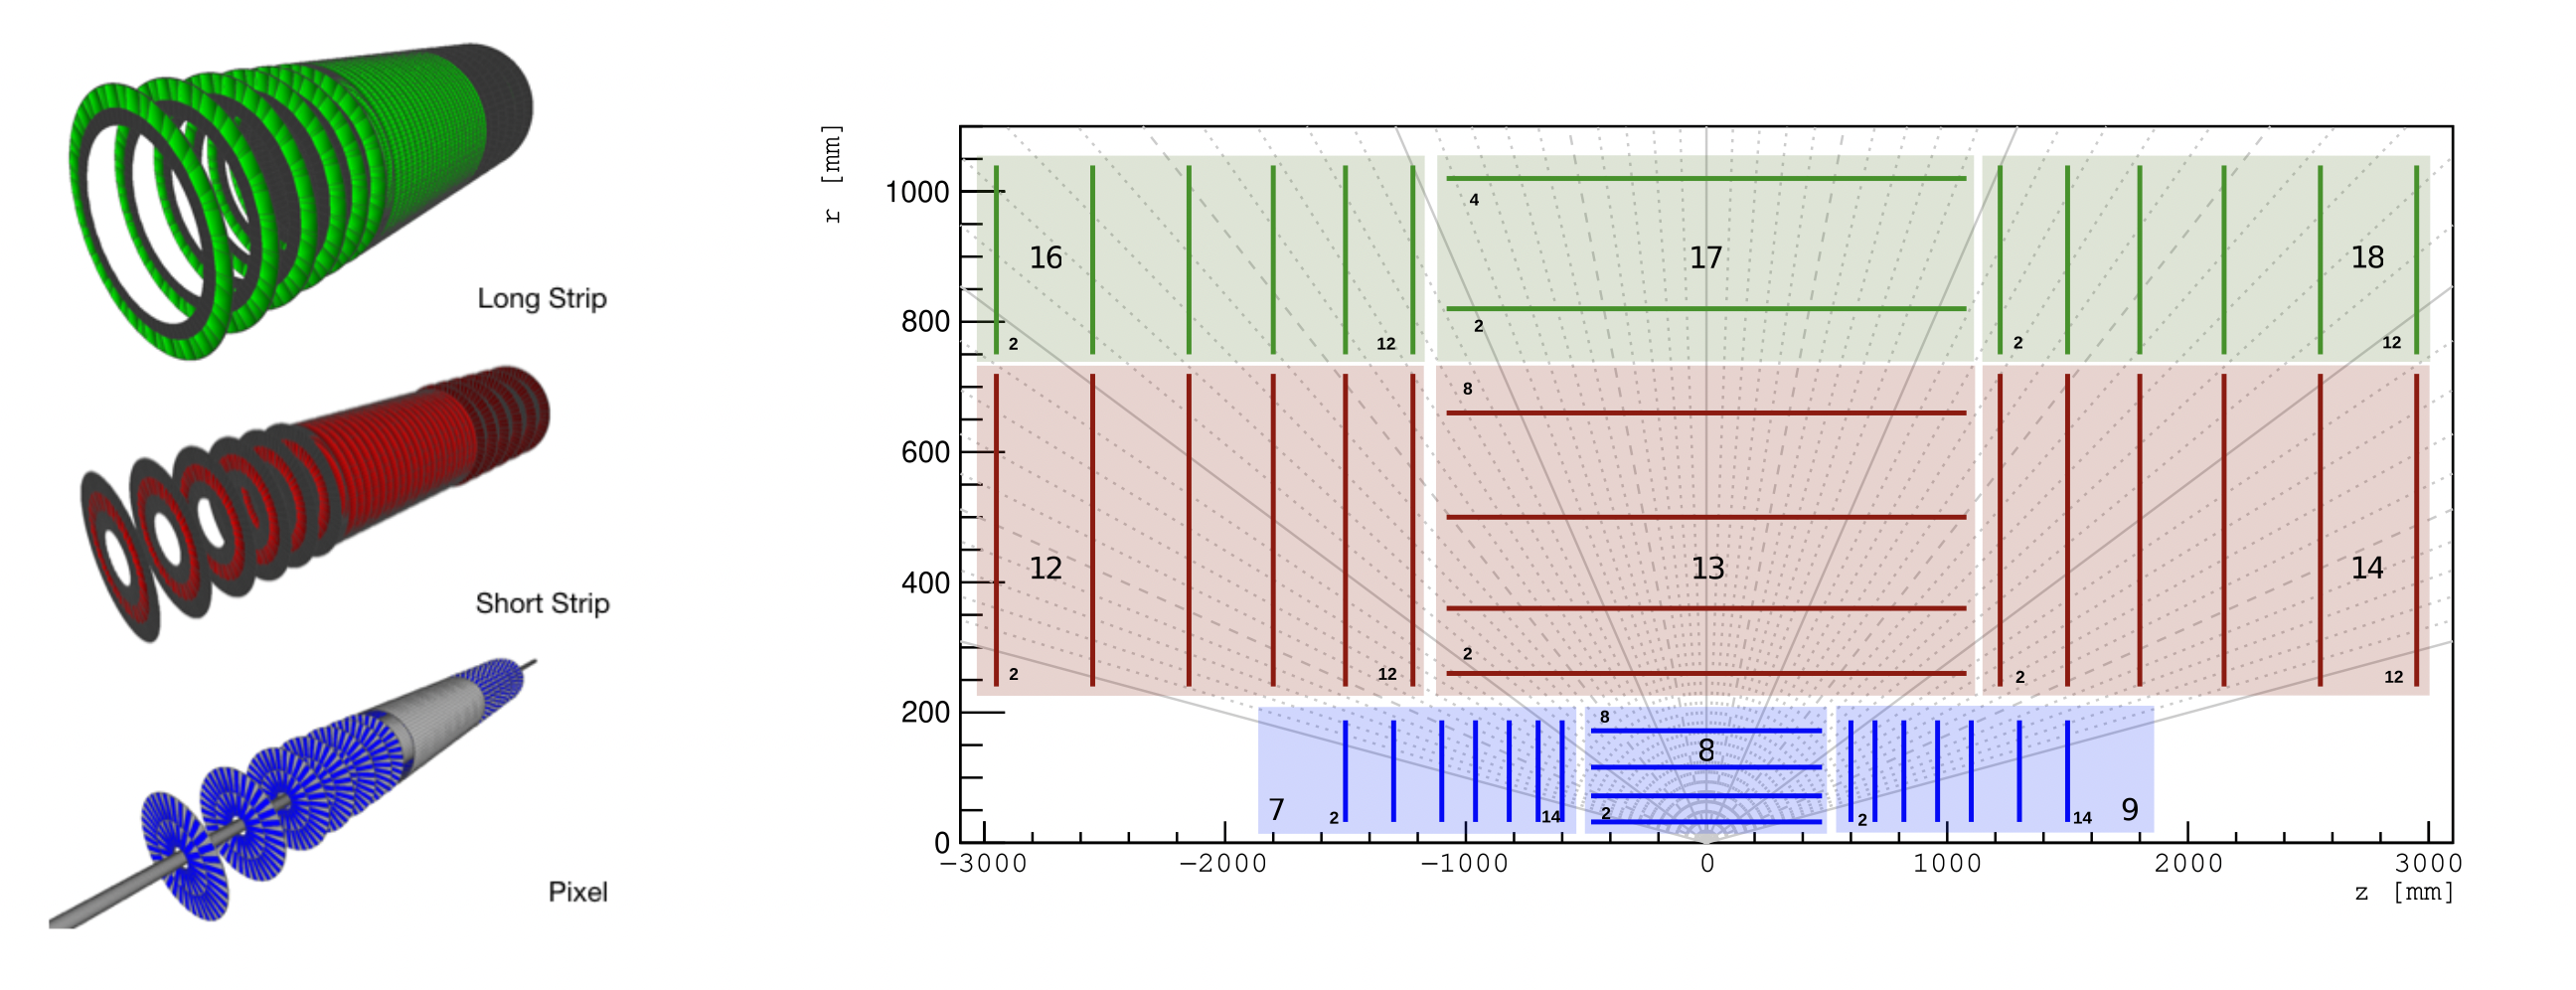
\includegraphics[width=\textwidth]{images/3-track-reconstruction/trackml-detector.png}
  \caption{
    Detector layout for the virtual TrackML detector. On the left the three major sub-detectors, pixel, short strips, and long strips, are shown separately. On the right, a schematic of the full layout and its coverage along the radial and longitudinal dimensions as well as in the $ \lvert \eta \rvert$ direction is shown. The different colors represent the different sub-detectors while the marked numbers are the internal volume and layer identifiers.
  }
  \label{fig:trackml-detector-image}
\end{figure}



The detector is split into three separate sub-detectors that differ in spatial resolution and passive material. The innermost sub-detector is a pixel detector with a spatial resolution of 50 $\mu$m $\times$ 50 $\mu$m and further out two different strip detectors with short 80 $\mu$m × 1200 $\mu$m and long strips 0.12 mm $\times$ 10.8 mm are placed. Each detector includes realistic module geometries with placement and overlap chosen to yield a hermetic coverage up to $\lvert \eta \rvert$ = 3. The particle beams collide on the $z$-axis around z = 0 mm. This is the centre of collision and also the centre of the detector. The TrackML detector is also organized into groups of layers, called \textit{volumes}, which are identified by a volume number. The pixel detector is represented by volumes 7, 8 and 9.

%ITK: There is no reason to believe the more complex geometry would lead to radically different algorithms

%The TrackML detector also shares several interesting features with the ATLAS detector, for example its solenoid parameters are the same and ....

%Instead of using the proposed upgrade tracker designs of either ATLAS or CMS we opted to design a generic tracker design that takes the key concepts from the existing proposals. This avoids issues of private collaboration information or artefacts and allows a challenge that is more separated from the particular design choices made by each experiment.

% -------------------------------
%More details in the documents on the TrackML competition:
%https://hal.inria.fr/hal-01745714/document
%https://arxiv.org/pdf/1904.06778.pdf
% ------------------------------


\subsection{Event Simulation}
\label{trackml-simulation}
%10.1051_epjconf_201921406037.pdf
The particle content of the collisions is generated using the Pythia 8 event generator \cite{pythia-8}. Pythia is a standard tool for generation of high-energy collisions, and contains a library to model hard scatter processes as well as the initial and final state of parton showers. A hard Quantum Chromodynamic (QCD) interaction that generates a $t\bar{t}$-pair (top quark and top antiquark) is used as the signal. An additional $\langle \mu \rangle$ = 200 soft QCD interactions (Poisson distributed) are overlayed to simulate the expected pile-up conditions at the HL-LHC. Charged particles are propagated through the detector using a fast detector simulation based on the ACTS software \cite{Gumpert_2017}. A non-homogeneous magnetic field is used, similar to the one in ATLAS, and material interactions, i.e. multiple scattering, energy loss, and hadronic interactions, are simulated using parametric models. Only tracks with a transverse momentum above 150 MeV are propagated. Tracks below this momentum threshold are typically not considered by the HL-LHC experiments.

% top quark decays: https://en.wikipedia.org/wiki/Top_quark

\subsection{Challenge Summary and Outlook}
\label{trackml-key-findings}

The TrackML competition exposed a diverse range of ML approaches, where accuracy and throughput were used to categorise the best algorithms for track reconstruction. The performance of the algorithms are evaluated using track purity and particle purity, for tracks originating from primary particles produced in the actual pp collisions. The purity is defined as follows; each track is matched with the ground truth majority particle sharing with it the greatest hit number, $N_{truth}$. The ratio of $N_{truth}$ to the number of hits of the reconstructed track, $N_{hits}$, defines the track purity, while the ratio of $N_{truth}$ intersection to the number of hits of the underlying particle, $N_{phits}$, defines particle purity. The quality of the top performing algorithms were analyzed in further detail. It was found that methods based on track following techniques are highly effective at reconstructing tracks globally with high purity, in comparison with clustering based approaches. 

Amongst the top ranking solutions, the developed algorithms were highly inspired from traditional track following approaches, such as the procedure outlined in Section \ref{track-reconstruction}. A short review of the submitted solutions that are influential to the research presented in this thesis is provided.

\subsubsection{TopQuarks Algorithm}

The winning algorithm proposed by the \textit{TopQuarks} team is based on a modular track following strategy, where the definition of a track is given by a sequence of hits. It begins with seed generation selected from hit pairs (doublets) in the innermost layers of the detectors. A logistic regression classifier is trained on doublet features and allows to reduce the number of fake seeds. The logistic classifier typically utilises the sigmoid function taking input and classifying it as a continuous output, representing the probability of good doublet prediction. The doublets are then extended to triplets via a further logistic classifier trained on triplet features. Track following is then implemented using a helix extrapolation and track ambiguity resolution is executed to remove polluting hits. The TopQuarks solution achieved approximately 95\% track reconstruction efficiency during the accuracy phase of the competition, with both its track purity and particle purity defined as $> 50\%$, as per the competition definition.

% Tracks are then consolidated by taking into account any hits located on overlapping modules if they are closer than a defined threshold.

\subsubsection{Outrunner Algorithm}

Another high-ranked algorithm is proposed by the \textit{Outrunner} team, based on training a multi-layered perceptron (MLP) to predict whether any two hits that are connected to the same track, where the definition of a track is the same as above. All pairs of hits were considered and 27 input features were constructed from its quantities. A neural network model composed of multiple wide dense layers is trained to predict the probability of the pair to be on the same track, hence predicting the adjacency matrix of network connections. The proposed approach is an unstructured track following algorithm where the next hit is not provided by track extrapolation, but directly by a hit index based on the hit pair classifier score. This suggests that too many branches of the combinatorial tree are followed during the track following step. The Outrunner solution achieved $> 90\%$ track reconstruction efficiency during the accuracy phase of the competition, and both its track purity and particle purity defined as $> 50\%$, as per the competition definition.

% There is a large class imbalance in the problem due of the predominance of pair of hits that are not belonging to the same track. This is overcome by sampling pairs from the negative class closer to the positive pairs to better define the boundary between the two classes. The accuracy weighted by the class cardinal is a better estimator of the performance of the model in this heavy imbalanced setup.

\subsubsection{Other Proposed Solutions}

Another team used various techniques based on the famous clustering-based approach DBSCAN (Density-Based Spatial Clustering of Applications with Noise) \cite{dbscan}. The idea of the DBSCAN-based algorithm was to find a subspace of track parameters in which a good track could be represented as a point-like object in this subspace. It is a popular clustering algorithm used commonly in data analysis and pattern recognition. It groups data points based on their density, identifying clusters of high-density regions and classifying outliers as noise. Track candidate building is executed using doublet track parameters, such as curvature and longitudinal impact parameters, within the DBSCAN clustering. This type of transform is a highly complex task and despite a best effort, the proportion of good tracks reconstructed was $\simeq$ 50\%. 

An alternative methodology implemented by another team utilises a Recurrent artificial Neural Network (RNN) using Long Short-Term Memory cells (LSTM). In contrast to uni-directional feed-forward neural network, RNNs are bidirectional, meaning that they allow the output from certain nodes to affect subsequent input to the same nodes. Their ability to use internal state (memory) to process arbitrary sequences of inputs makes them applicable to tasks such as sequence data. The LSTM mechanism provides a short-term memory for the RNN that can last thousands of timesteps, and as such RNNs can keep track of arbitrary long-term dependencies in the input data. The ability of RNNs to capture temporal dependencies makes them well-suited for tasks such as language modelling and sequential data analysis. Both RNNs and GNNs exploit a similar processing framework, but they can be applied to different input domains. Typically, RNNs require the input graphs to be directed and acyclic, whereas GNNs can process any kind of graph structure, making them versatile in nature and applicable to more complex problems.

The proposed solution to the TrackML challenge begins with seed building, where the DBSCAN algorithm is used to cluster hits in the inner-most layers of the detector in order to produce tracklet seeds. The RNN is then used within the path prediction stage in place of a propagator (such as a traditional KF track following algorithm) to find the potential position of hits on subsequent layers of the detector. The RNN model is trained using multiple architectures and used to predict the positions of the next hits, however the training of the models is quite prohibitive to allow for a full optimization due to its computational load. The proportion of good tracks reconstructed from this algorithm was $\simeq$ 85\%. More information about the details of the competition criteria, analysis and algorithm breakdown can be found in \cite{Amrouche_2019}.


\subsubsection{Motivation for Graph Neural Network Approach}
Several approaches highlighted by the TrackML challenge show great promise for accurate track reconstruction. However, in realistic detector setups, the physics reach of particle detectors will be limited by how efficiently the experiments can use their available computing resources. Many of the teams which applied deep learning to the vast amount of training data in the challenge faced computation resource limitations. Even with the use of general purpose Graphical Processing Units (GPUs), training of the models took multiple days. These approaches would not be suitable to implement in the software for realistic detectors.

In addition, approaches that heavily rely on the use of clustering are also not effective for realistic detectors. Clustering-based techniques require finding a parameter space where tracks exist as point-like objects. If a detector model contained a perfect uniform magnetic field and there were no material effects present, the behaviour of tracks in such a parameter space could be easily modelled as points and hence algorithms such as DBSCAN would be highly effective. However, this is not the reality due to multiple scattering effects. Clustering-based approaches are widely used to combine hits into doublets and extend doublets to triplets, however they are not the most successful when used to reconstruct tracks globally. The above factors were considered when exploring an alternative route. 

In recent years, algorithms for track pattern recognition based on GNNs have emerged as a particularly promising route. The authors of Ref. \cite{farrell2018novel} identified the use of GNNs as a promising solution for charged particle tracking at the HL-LHC. Since this publication, significant effort has been invested in the development of algorithms based on GNNs. One method in particular focuses on establishing a method based on training MLPs and employing deep learning techniques through GNN application and is the work done by the Exa.TrkX project \cite{ExaTrkX-website, Caillou:2815578}. Excellent performance of this GNN-based algorithm on the TrackML dataset \cite{refId0} has been demonstrated in Ref \cite{Ju_2021} and further information on this application is discussed in Section \ref{track-recon-graph-networks}. In contrast to the approach taken by the Exa.TrkX project, presented in this thesis is a novel methodology developed for track reconstruction using GNNs, without employing deep learning techniques. Prior to presenting this approach, an introduction to graph network architectures is given in Section \ref{graph-networks}.


%From the ML point of view, the problem can be treated as a \textbf{latent variable problem} similar to clustering, in which particle trajectory “memberships” must be inferred, a \textbf{tracking problem} considering trajectories as time series, or a \textbf{pattern de-noising problem} considering that the dotted trajectories are noisy versions of continuous traces. As a result the competition exposed a diverse range of ML approaches.

% One important point is that the points on one trajectory are not geometrically close to each other (a human cannot associate the points by eye), but they follow a specific pattern : a distorted arc of helix pointing approximately to the origin.

% Tracking efficiency is commonly defined in particle physics as the probability to reconstruct a track. A good tracking algorithm must provide consistently high efficiency over a wide range of track parameters.


%--------------------------------------------------
%	Chapter 3: Graph Networks
%---------------------------------------------------
\section{Graph Network Architectures}
\label{graph-networks}

Graph network structures are data representations that describe objects and their pairwise relationships. Graphs are able to effectively capture complex relationships and dependencies between such objects, both on a local scale and globally. This is essential for accurately representing physical data and understanding the interactive behaviour of the network. As a result, GNNs can represent many types of relational and geometric data. Due to their great expressive power, GNNs have been applied in numerous different applications. They have emerged as the de facto standard for many geometry-heavy applications, such as molecular property prediction within drug discovery and social network analysis.

As graph-based architectures are a natural way to represent tracks, they have shown substantial promise for a variety of particle physics tasks. This includes track reconstruction and simulation. Section \ref{properties-graph-networks} presents the properties and common terminology used within the domain of graphs networks and Section \ref{track-recon-graph-networks} compares the track reconstruction methodology developed in this thesis, with a similar approach by the Exa.TrkX collaboration.

%In some cases, GNNs have demonstrated better scaling properties, reduced resource utilization and increased opportunity for parallel implementation compared to traditional methods.

% Useful links!!
% https://www.datacamp.com/tutorial/comprehensive-introduction-graph-neural-networks-gnns-tutorial
% https://distill.pub/2021/gnn-intro/


%--------------------------------------------------
%	Chapter 3: Properties of graph networks
%---------------------------------------------------
\subsection{Properties of Graph Networks}
\label{properties-graph-networks}

%\subsubsection{Graph Network Architecture}

A graph $\mathcal{G}$ is defined by a set of \textit{nodes} \{V\} (or vertices) and a set of \textit{edges} \{E\}. Nodes represent entities or objects and edges are connections between two nodes that model their pairwise relationship. These edges can be directed, non-directed and/or weighted, see Figure \ref{fig:graph-architecture-example} for example illustrations. The connectivity of a graph can be visualized through its adjacency matrix $A \in \{0, 1\}$, of size $n_{nodes} \times n_{nodes}$. If two nodes share an edge, then the corresponding entry in the adjacency matrix is populated with 1, and zero otherwise. 

The data from a tracking detector for a given event can naturally be represented using a graph. A node can represent a hit (or a group of close proximity hits) with each node containing attributes such as spatial coordinates, and the existence of an edge between two nodes indicates that the nodes could potentially represent two successive hits on a track. At the HL-LHC, $O(10^{5})$ hits per $t\bar{t}$ event are expected. A fully connected graph of such an event would have $O(10^{10})$ edges, most of them representing unphysical connections. Therefore, a key feature within graph construction is the choice of compatible edges. 

\begin{figure}[!htbp]
  \centering
  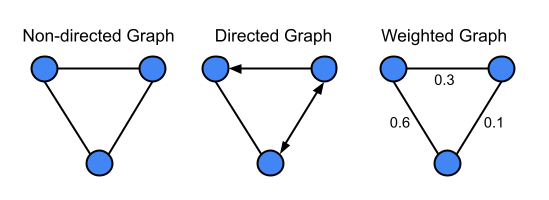
\includegraphics[width=0.85\textwidth]{images/3-track-reconstruction/Graphs.png}
  \caption{
    Illustration of different graph types. Non-directed graphs contain edges with no direction. Directed graphs can contain edges with unidirectional or bidirectional edges. Weighted graphs associate a weight to each edge, the example above has normalised edge weights. All three graphs are fully connected, whereby a unique edge connects each pair of nodes.
  }
  \label{fig:graph-architecture-example}
\end{figure}


\subsubsection{Message Passing Paradigm}

Message passing is an important property in the design of graph networks. It allows the propagation of node features by exchanging information between adjacent nodes. The edges between nodes act as conduits, allowing the transfer of information in a given direction if the connection is active. Typically, this scheme is iterative in nature. It begins with an initialization of a state at each node in the network, where a state typically comprises node or edge features. The node, $v$, then aggregates states from adjacent nodes in its local neighbourhood. Node representations are then updated based on an aggregation function, improving the precision of states local to each node. This process is then repeated with further message passing and neighbourhood information aggregation, allowing local information to spread globally throughout the network. GNNs can fully exploit the connectivity of their structure, and as a result the mechanism allows models to become sophisticated in learning rich and expressive representations of nodes that incorporate both local and global behaviour.


%--------------------------------------------------
%	Chapter 3: Track reconstruction on graph networks
%---------------------------------------------------
\subsection{Track Reconstruction using Graph Networks}
\label{track-recon-graph-networks}

The ExaTrkX collaboration \cite{ExaTrkX-website} has proposed an approach for track reconstruction using GNNs \cite{Caillou:2815578}. This graph-based algorithmic pipeline has two main stages, the first being graph construction and the second being track finding. Their approach represents a particle collision as a collection of nodes and edges. Each hit is treated as a node, which encodes features such as spatial position, and nodes are connected by edges that represent the possibility of two nodes belonging to the same track. Their goal is to use ML and graph techniques to segment or cluster the nodes to match particle tracks. The construction of the graph network is executed by training a MLP for edge classification by predicting edge scores, where message passing is used within the network to improve the discrimination power of the classifier, as well as a metric learning approach. Track finding is then done through deep learning approaches by training the GNN, as well as a graph segmentation process utilizing connected components and edge classification.

The proposed approach by the ExaTrkX project requires the use of deep learning techniques, which can result in the enormous use of computational resources. Considering the work developed by ExaTrkX, as well as the ideas which stemmed from the TrackML challenge, this has inspired the research presented in this thesis. 

Showcased here is a novel methodology exploring the use of a GNN architecture as a solution to the track pattern recognition problem, without the use of traditional deep learning techniques. The procedure developed here is somewhat of an intermediary of the described algorithms submitted to the TrackML challenge in Section \ref{trackml-key-findings}, as well as the incorporation of new techniques. The GNN-based model presented in this thesis is used to model tracks as sequences of points in a parameter space and simultaneously allows the natural structure of particle trajectories to be embedded into its architecture. 

There are two main aspects to this approach; a procedure to construct a graph network is presented in Chapter \ref{chapter-4} and a method to refine its connections and extract tracks is presented in Chapter \ref{chapter-5}. In order to identify compatible connections, a ML-based algorithm is used to predict if two hits belong to the same track, given input hit features, such as the charge distribution in the cluster. The training involved in this procedure is such that functions used to calculate track state parameters are learned, without using deep learning or vast computational resources. This approach ensures a realistic implementation for detector experiments. Following this, an iterative procedure allows ambiguities in the network to be identified and tracks to be isolated. To efficiently exploit a priori knowledge about charged particle dynamics the GNN-based algorithm uses simplified KFs as mechanisms for information propagation as well as for track extraction. Further information is given in Chapters \ref{chapter-4} and \ref{chapter-5}.
%--------------------------------------
%	Chapter 4. ML Hit-Pair Predictor
%--------------------------------------

%\doublespacing
%\newpage
%\setcounter{section}{3}
%\section{The Compressed Pattern Space}
\chapter{Machine Learning Hit-Pair Predictor} 
\label{chapter-4}
% DONE


% This study was conducted in order to speed up the track seeding stage and reduce CPU time in the ATLAS fast tracking trigger algorithm.

When constructing graph networks for track reconstruction, one must first consider the ability to identify compatible hit connections to build graph edges. A beneficial step towards enhancing this process is to reduce the number of fake edges constructed and hence increase the accuracy in predicting such compatible hit-pairs. As future upgrades to particle detectors will lead to significant increases in hit occupancy, this will be problematic for silicon tracking detectors. Therefore, it is essential that resource use is also considered, whilst maintaining the capability to reconstruct tracks with minimal efficiency loss. This chapter presents a methodology to accomplish such a task. This work is presented in the Journal of Physics: Conference Series \cite{Lad_2023} and is implemented in the optimisation of the HLT ID track seeding software for ATLAS Run-3 and beyond \cite{Grandi:2728111, Long:2813981}. Section \ref{measurement-to-track-association} presents the development of a ML-based algorithm to predict if a pair of hits belongs to the same track given input hit features, namely cluster width and inverse track inclination. The implementation of the trained predictor in the form of Look-Up Tables (LUTs) is presented in Section \ref{application-of-hit-pair-predictor}. Performance results, including tracking efficiency and speed-up factor are measured using simulated data and discussed.


\section{Measurement to Track Association}
\label{measurement-to-track-association}

\subsection{Data Exploration and Feature Extraction}

Seeds constructed at the combinatorial stage of ATLAS tracking software designed for the Run-2 geometry were used to extract hit-pairs to form a training dataset. Monte Carlo (MC) $t\bar{t}$ event samples with centre-of-mass energy $\sqrt{s}$ = 13 TeV at mean pile-up interaction multiplicity $< \mu >$ = 80 were used. Top quark simulation is often used for developing algorithms in tracking due to its many possible final states including electron, muon and $\tau$ leptons, as well as hadrons. Due to the presence of pile-up, the multiplicity of constructed seeds is high. A larger proportion of fake seeds will be naturally present, so that $t\bar{t}$ with pile-up provides a good description of the environment in high luminosity conditions.

The training is focused on Pixel detector layers, being closest to the beamline and having highest hit occupancy. An illustration of a seed in the ID Pixel layers is shown in Figure \ref{fig:triplet-illustration}. The input seeds are triplets of spacepoints which are deconstructed into pairs of doublets sharing a common middle spacepoint. For each seed, the inner doublet (defined as hit-pair 1 and 2) and outer doublet (defined as hit-pair 2 and 3) are extracted. The total number of Pixel barrel and Pixel endcap hit-pairs extracted were 365,937 and 18,537 respectively. For each hit-pair, the absolute inverse slope of the track, $|\cot(\theta)|$, is calculated using $r$-$z$ coordinates and used as an input feature for training. $\theta$ is the angle of inclination of a hit-pair with respect to the $z$ axis. The longitudinal Pixel cluster width, $w_{\eta}$, measured in the $\eta$ direction was also extracted, where $\eta$ is defined in Eq. \ref{eq:pseudorap}. The MC-generated data in the [$|\cot(\theta)|$, $w_{\eta}$] phase space behaves as a set of 1-dimensional distributions, each with discrete $w_{\eta}$. This is a direct result of charge deposition over a grid of pixels in the simulated Pixel modules. The geometry of Pixel modules are subdivided into majority \textit{standard} pixels of width 400$\mu$m and 10\% of \textit{long} pixels of width 600$\mu$m. The long pixels are responsible for covering the gap between the front-end chips on the modules and provide full coverage \cite{pixel-module-dimensions}. Hence, the discrete cluster widths are observed to be increasing in increments of 200$\mu$m. This characteristic is exploited to form an ensemble of predictors. 

The MC truth information for seeds and their corresponding hit-pairs were extracted from ATLAS tracking software and used as targets in training. Doublets where both hits belong to the same truth track were labeled as truth 1 (correct hit association). Conversely, doublets where both hits do not belong to the same truth track were labeled as truth 0 (incorrect hit association). Hit-pairs for the Pixel barrel and endcap are handled separately in order to build regional classifiers. Hit-pairs located in the transition region of the ID belonging to both barrel and endcap layers are automatically assigned to the barrel classifier. This decision was made such that seeds which would be rejected in the barrel would differ from seeds rejected in the endcap, hence the classifiers would cover a wide proportion of fakes. Therefore the location and track inclination of the innermost hit is considered and the hit-pair is assigned to the corresponding classifier. However, the handling of these doublets can be improved. The same methodology was used for both the Pixel barrel and endcap, and are presented in Section \ref{section:classifier-dev} and \ref{application-of-hit-pair-predictor}.

% For seeds where one doublet's hits is completely located in the barrel i.e. both hits are barrel-barrel or completely located in the endcap i.e. both hits are endcap-endcap, and the other doublet in the seed is in the transition region (i.e. barrel-endcap), we look at the location of the middle spacepoint in the seed to determine which regional classifier this data should end up with. i.e. if the middle spacepoint is in the barrel and the outer spacepoint is in the endcap, then this data feeds into the barrel classifier. if the middle spacepoint is in the endcap and inner spacepoint is in the barrel, then this data feeds into the endcap classifier. 

% Maybe this is a flaw/limitation of how the transition region data between barrel and endcap are handled, and really this data should be included in both the barrel and endcap classifiers.



\begin{figure}[!htbp]
\centering
    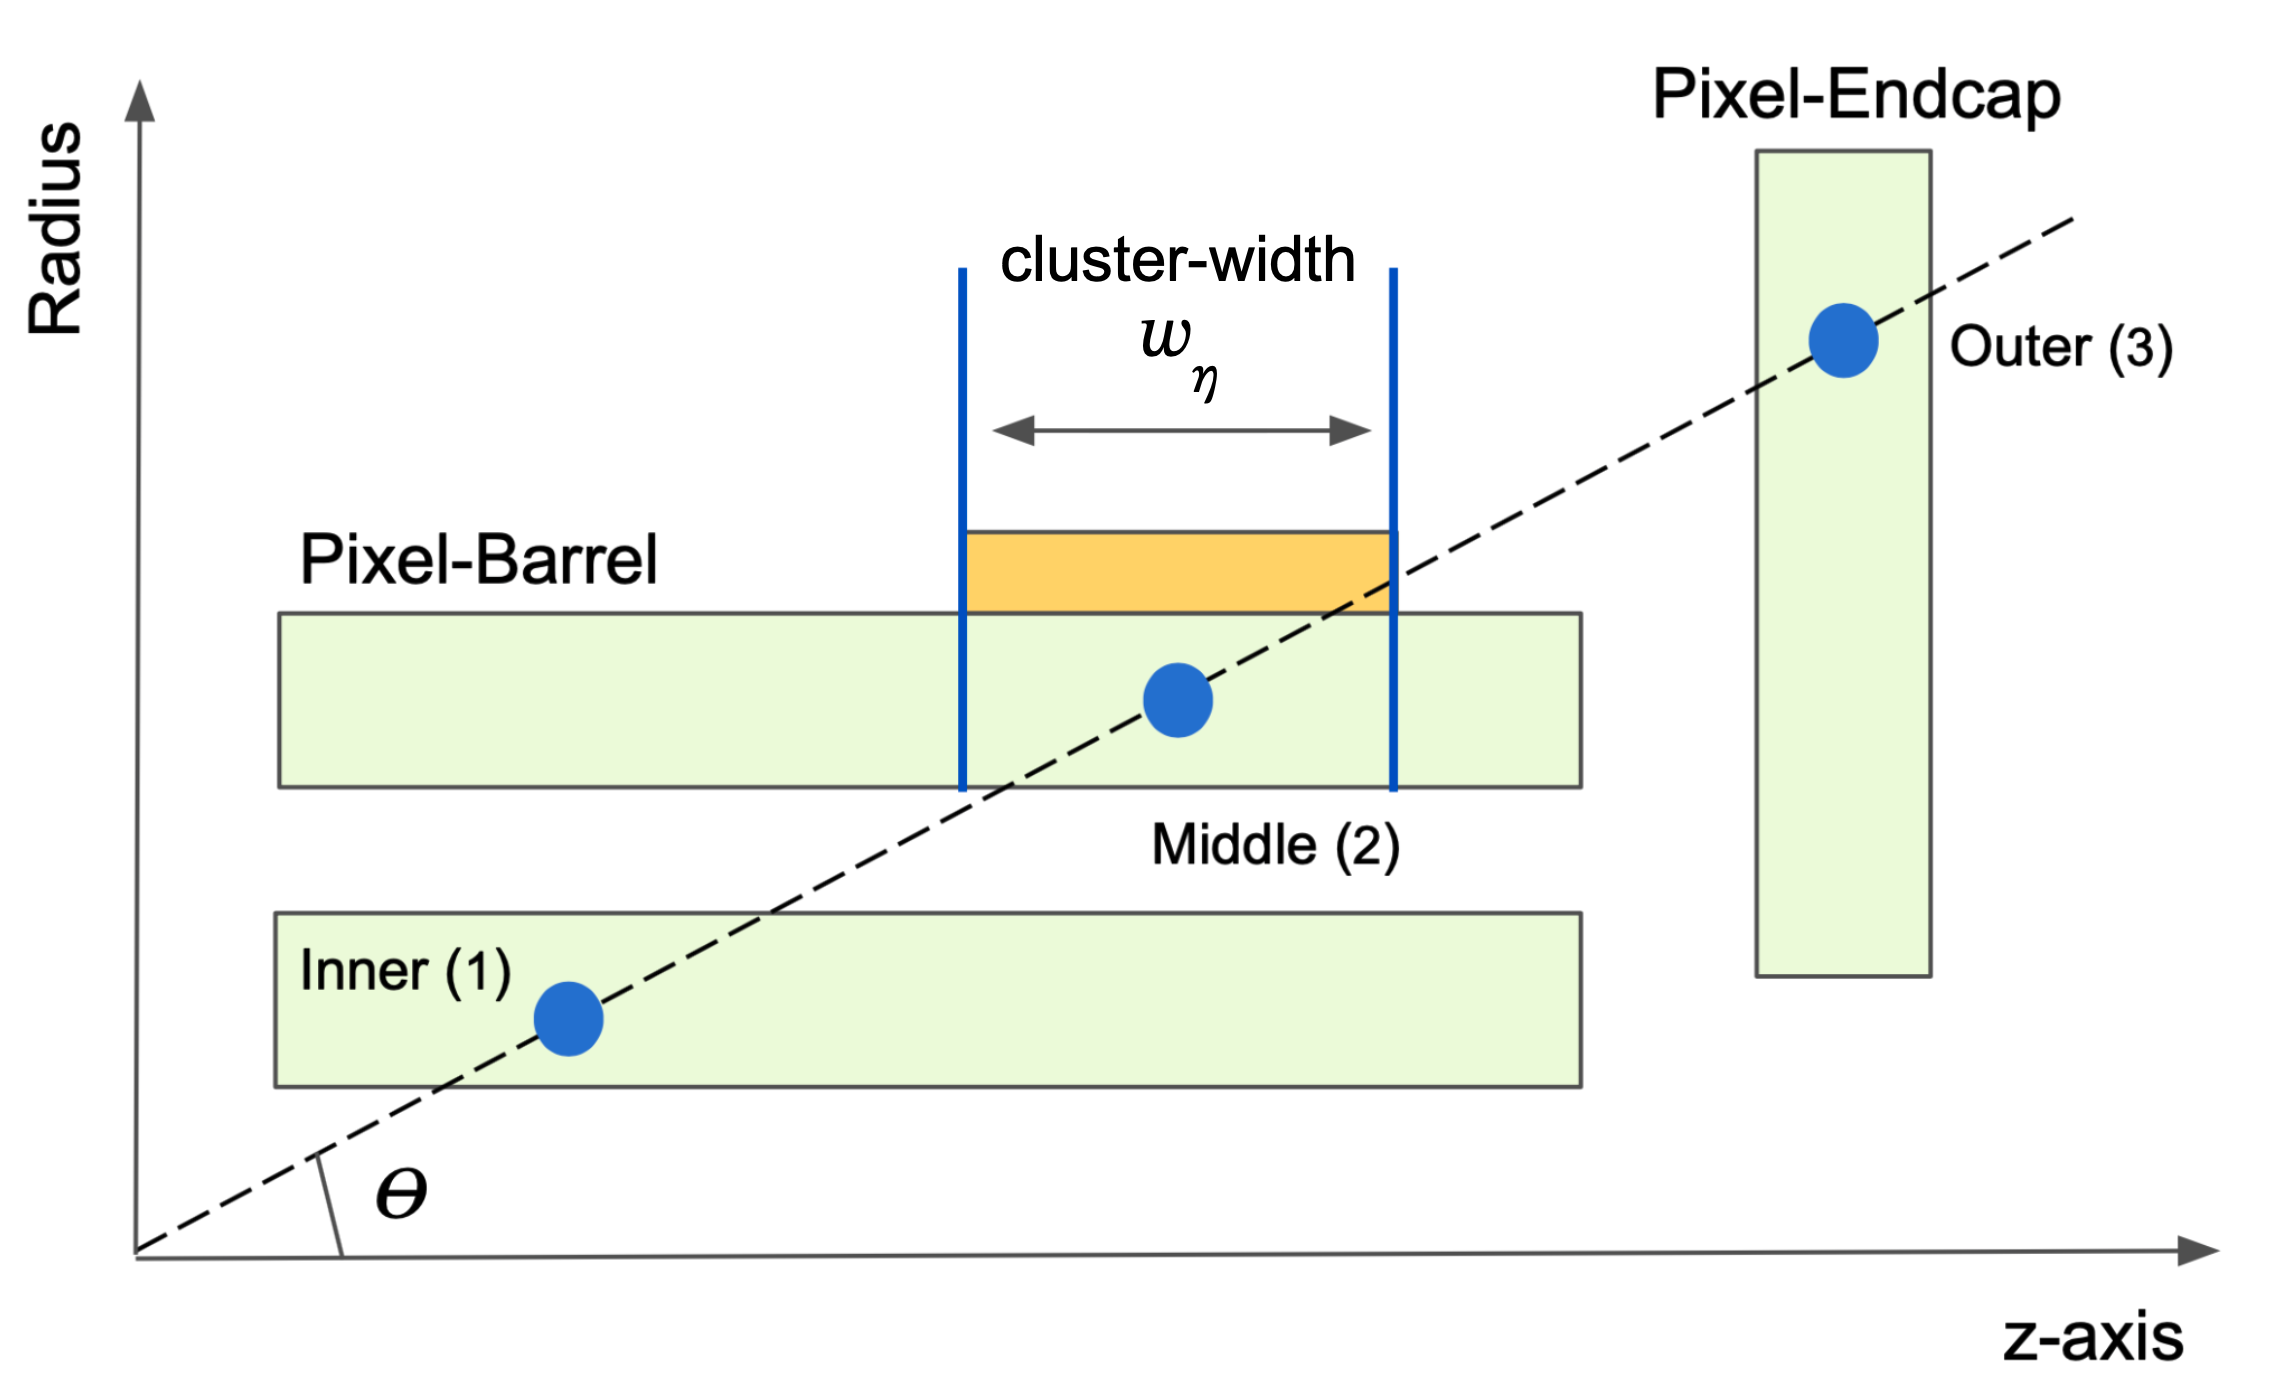
\includegraphics[width=0.85\linewidth]{images/4-ml-based-predictor/triplet_illustration_2.png}
    \caption{Seed illustration in the $r$-$z$ plane of the ID. The inner doublet consist of hits 1 and 2, and the outer doublet consist of hits 2 and 3. The longitudinal pixel-cluster width, $w_{\eta}$ (mm), is measured in the direction of $\eta$, where $\theta$ is the angle of inclination with respect to the $z$ axis.}
\label{fig:triplet-illustration}
\end{figure}


\subsection{Classifier Development}
\label{section:classifier-dev}

\subsubsection{Not-so-Naive Bayes}
% DONE

The basis of Bayes’ theorem \cite{naive-bayes} is used to build a classifier to discriminate between doublet classes, for both the Pixel barrel and endcap regions. Bayesian analysis is based on having a prior probability of belief of an outcome of an event and a likelihood probability, where naive Bayes’ assumes that the conditional probabilities of the independent variables are statistically independent. The final classification is produced by computing the posterior probability by combining both the prior beliefs and the likelihood, which then determines the most probable class label. Using Bayes’ theorem is advantageous in this data-driven setting, as prior knowledge of the behaviour of the system is known. The posterior probability $P(c|x)$ that a given data point x belongs to class c is defined as:

\begin{equation} \label{naive-bayes}
    P(c|x) = \frac{P(x|c)P(c)}{P(x)}
\end{equation}

where $P(x|c)$ is the conditional likelihood, $P(c)$ is the class prior probability and $P(x)$ is the predictor prior probability, used for normalisation and calculated from the number of data points belonging to class $c$. Bayes' theorem is implemented using a generative model for each class. This was achieved by computing the likelihood function via a Kernel Density Estimate (KDE) for each of the 1-dimensional $|\cot(\theta)|$ distributions, forming a set of generative Bayesian classifiers. This method removes the 'naive' element and performs the same classification with a more sophisticated generative model for each class.

\subsubsection{Kernel Density Estimation}
% DONE

KDE is a non-parametric approach to estimate the probability density function of a random variable. The idea is that a kernel function is defined and centred on each data point in the sample. The sum of these functions together forms the kernel density estimate. The kernel density is defined as:
    
\begin{equation} \label{eq2}
    \hat{f}(x) = \frac{1}{Nh}  \sum_{i=1}^{N} K \left( \frac{x - x_i}{h} \right)
\end{equation}

where $K(x)$ is the kernel function, typically a smooth, symmetric and non-negative function, $h > 0$ is the smoothing bandwidth that controls the amount of smoothing applied to the function and N is the number of sample points used for normalisation \cite{kde}. One advantage of using KDE is that it provides a more flexible estimator parameterised by $h$. The KDE must be normalised in order to represent a probability density. For this study, the Gaussian kernel function was used to approximate the probability density at each data point in the sample. The area under a Gaussian curve is symmetrical, which is an appropriate regularisation. The Gaussian kernel is defined as:
    
\begin{equation} \label{eq3}
    K(x) = \frac{1}{\sqrt{2\pi}} e^{\frac{-x^2}{2}}
\end{equation}

The choice of bandwidth is important, as too large bandwidth results in a distribution where granular information is lost (over-smoothing). Conversely, a bandwidth that is too small, can lead to narrow peaks in close proximity to each other, resulting in a very noisy distribution (under-smoothing). There are several methods to determine the optimum bandwidth discussed in \cite{bandwidth-selection-methods}, many of which show similar properties. The method used in this study was the so-called \textit{Silverman's rule of thumb}, which works only for 1-dimensional data. Silverman's rule finds the bandwidth that minimizes the mean integrated squared error assuming that the data is Gaussian and a Gaussian kernel was used.

\newpage
\subsection{Classifier Training}
% DONE

The hit-pair data was separated into a training and a test dataset using a 70:30 split. The training data was analysed in the phase space of [$|\cot(\theta)|$, $w_{\eta}$]. Figure \ref{fig:truth-histo} shows an example of the 1-dimensional distributions of $|\cot(\theta)|$ for Pixel barrel hit-pairs with $w_{\eta} \le$ 0.4mm, where a clear distinction is observed between each truth class. The Bayes’ classifier was implemented in a generative way, computing the likelihood via a fitted KDE to each correct hit association distribution parameterised by $w_{\eta}$. The feature vector \textbf{x} comprised $|\cot(\theta)|$ and the truth label of the hit-pair formed the target vector \textbf{y}. For unknown data points, the class which maximised the posterior was the class prediction.

After training, the predictions from each classifier were adjusted using the model's corresponding Receiver Operating Characteristic (ROC) curve \cite{Davis2006-oh}. The ROC curve indicates the performance of the classification model at all classification thresholds, where each point on the curve corresponds to a prediction probability. The ROC curve plots two parameters: True Positive Rate (TPR, also known as recall) and False Positive Rate (FPR), defined as:  

\begin{equation}
    TPR = \frac{TP}{TP + FN}, \quad FPR = \frac{FP}{FP + TN}
\end{equation}

where TP (True Positive) indicates the number of truth 1 hit-pairs correctly classified by the model and FN (False Negative) indicates the number of truth 1 hit-pairs incorrectly classified. In other words, TPR measures the proportion of positive instances correctly detected as positive by the model. Similarly, FP (False Positive) indicates the number of truth 0 hit-pairs incorrectly classified and TN (True Negative) indicates the number of truth 0 hit-pairs correctly classified. The TPR and FPR are two important performance metrics commonly used in binary classification problems to evaluate the effectiveness of a model to distinguish between the two classes. 

The ROC curve for the classifier is trained on the distribution for $w_{\eta} \le$ 0.4mm is shown in Figure \ref{fig:roc-curve}. The classifier’s predictions were adjusted (also known as tuning) using the prediction probability derived from the ROC curve to yield a TPR of 0.95. Such a high TPR was chosen in order to maintain a high purity of correct hit-pairs. It is often more flexible to interpret probabilities than class predictions, as one is able to balance trade off concerns between FP prediction and FN prediction, and hence adjust thresholds.

The Area Under the Curve (AUC) represents a measure of separability and indicates the ability of a model to distinguish between classes. The value of the AUC is in the range 0.0 $\leq$ AUC $\leq$ 1.0, where AUC = 1 corresponds to perfect classification. The AUC achieved by the ML classifier for the $w_{\eta} \leq 0.4$mm distribution was 0.79. The ‘no skill’ classifier with AUC = 0.5 is also shown in Figure \ref{fig:roc-curve}. This classifier cannot discriminate between correct or incorrect hit association classes and would predict a random class in all cases with 50\% probability.


\begin{figure}[htbp!] 
    \centering
    \subfloat[]{%
        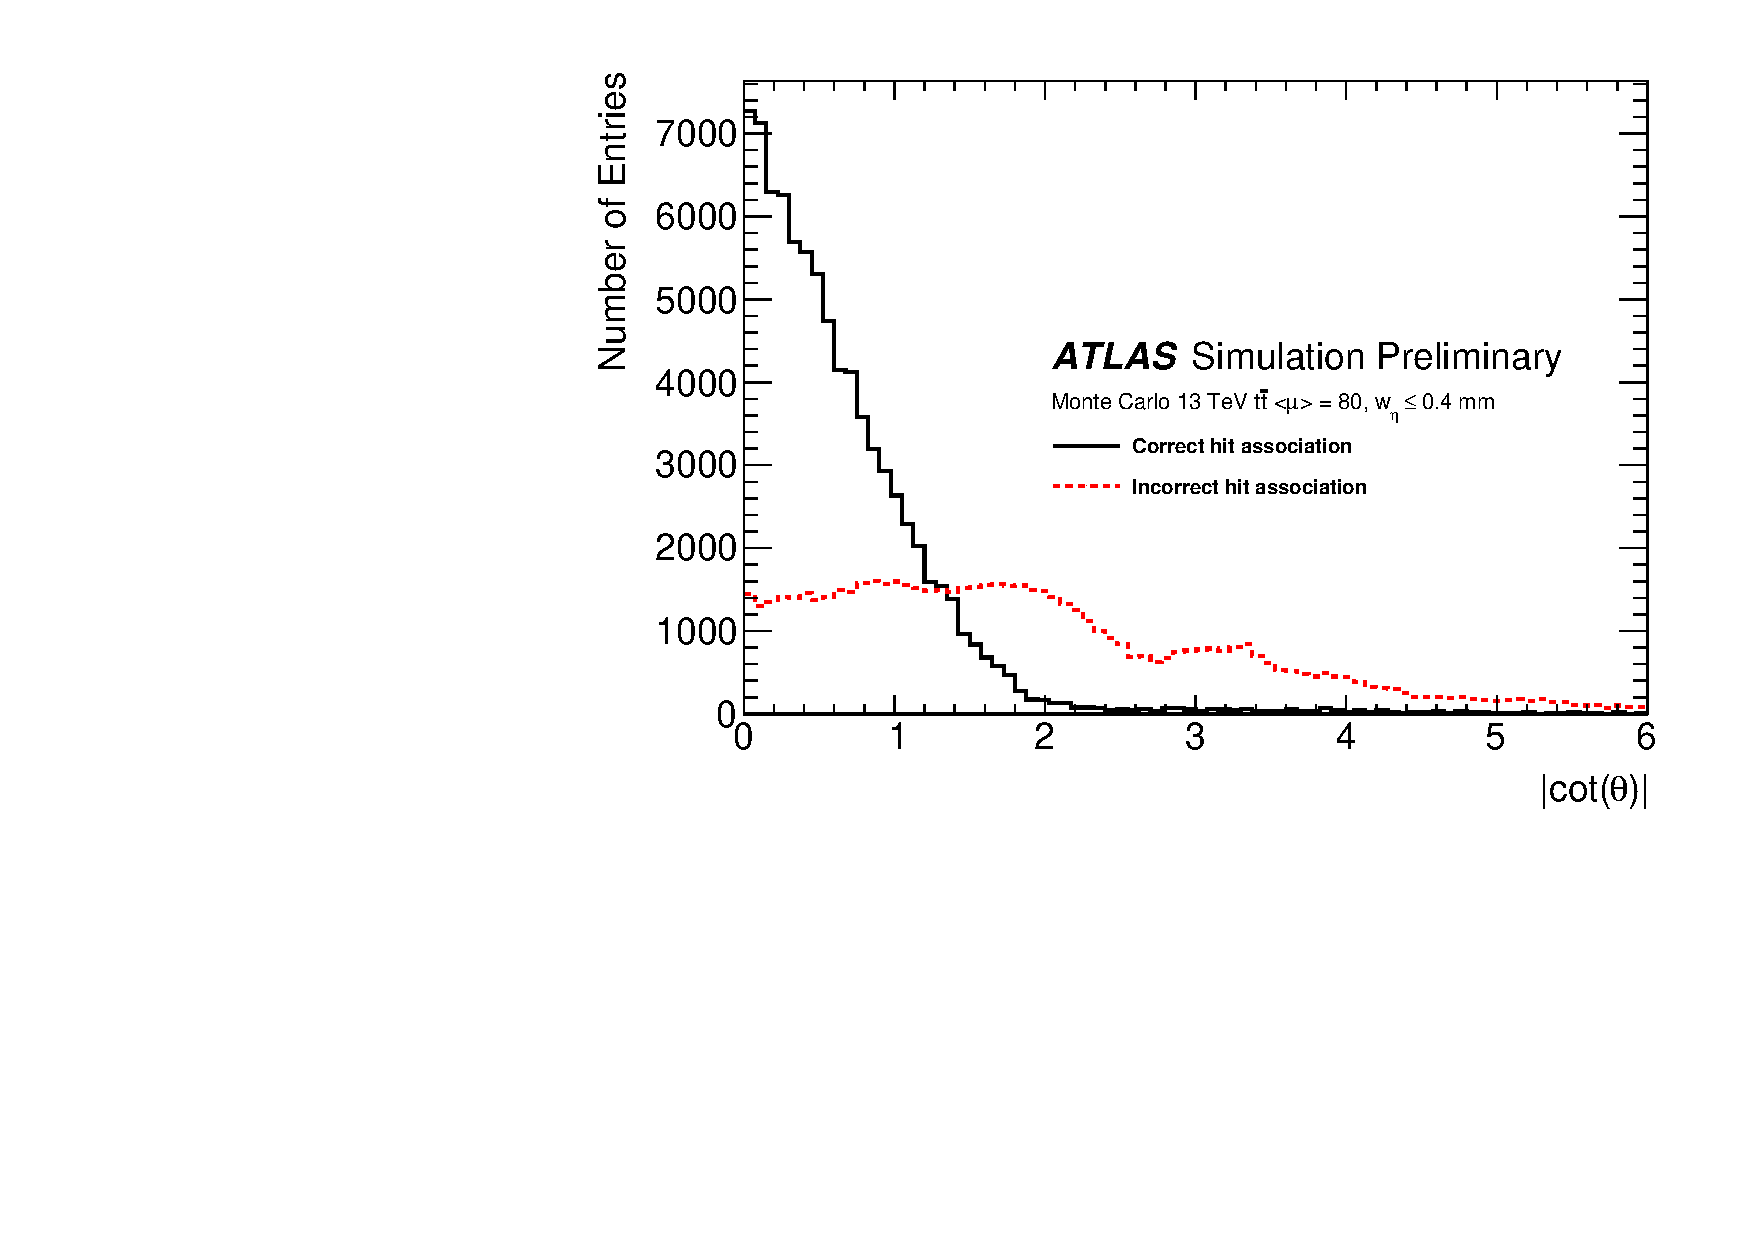
\includegraphics[width=0.98\textwidth]{images/4-ml-based-predictor/histo.pdf}%
        \label{fig:truth-histo}%
        }%
    \hfill%
    \subfloat[]{%
        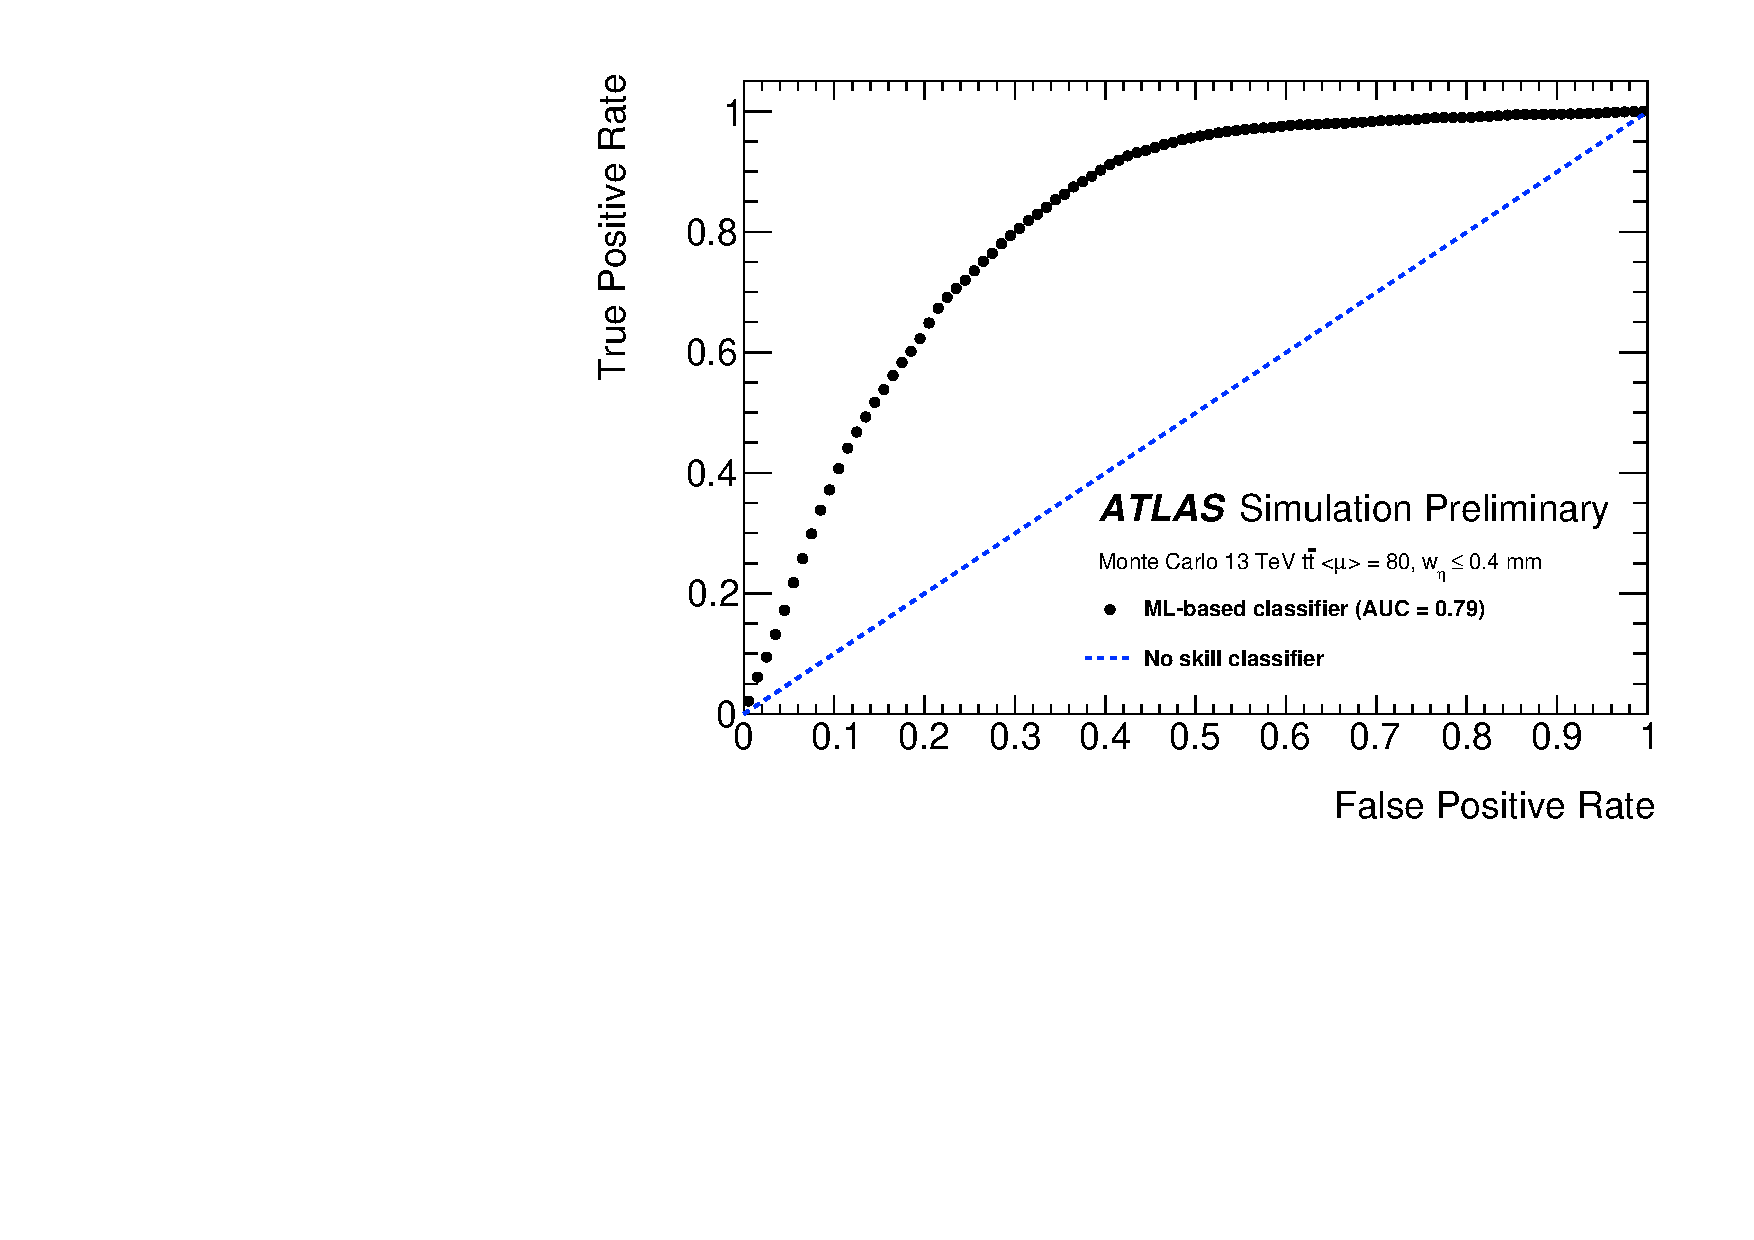
\includegraphics[width=0.98\textwidth]{images/4-ml-based-predictor/roc.pdf}%
        \label{fig:roc-curve}%
        }%
    \caption{(a) $\lvert \cot(\theta) \rvert$ for Pixel barrel hit pairs with $w_{\eta} \leq 0.4$ mm in the ATLAS Pixel detector, where $\theta$ is the inclination angle of the hit pair with respect to the $z$-axis. (b) The corresponding Receiver Operating Characteristic (ROC) curve for the classifier trained on the data shown in (a). The curve indicates the rates of false positive and true positive of Pixel barrel hit pairs to tracks corresponding to truth particles.}
    \label{fig:1-dimensional-classifier-training}
\end{figure}


\subsubsection{Probability Calibration}

% READ THIS:
% https://machinelearningmastery.com/calibrated-classification-model-in-scikit-learn/
% https://scikit-learn.org/stable/modules/calibration.html

Probability calibration can provide more nuanced ways to evaluate the performance of the model. The discrepancies between the predicted probabilities of each classifier and its relative observed frequency for the positive class were analysed. A well calibrated model produces predictions that, on aggregate are closely aligned with the actual outcomes, and hence should appear as a diagonal. Points below the diagonal indicate a model is typically over-forecasting and conversely points above the diagonal indicate under-forecasting. There are several methods of probability calibration \cite{prob-calibration}. An Isotonic calibration fits a non-parametric regressor, whilst a Sigmoid calibration corresponds to a parametric approach. Each method was applied for the discrete 1-dimensional distributions. The performance was evaluated using the Brier score: the mean squared difference between the predicted probability and the actual outcome. Figure \ref{fig:calibration} shows the calibration curve of the classifier for the $w_{\eta} \leq 0.4$mm distribution. Little difference was observed between the Brier score for the uncalibrated classifier and calibrated models. This was observed for all other 1-dimensional distributions in $w_{\eta}$. As a result, no additional probability calibration was applied during the development of the ensemble of KDE-based classifiers.

%KDE Calibration curve for pixel-barrel doublets with 0 - weta - 0.4. We can evaluate how well our model \& the predicted probabilities are calibrated. Calibration curve (reliability diagram) is generated for each weta bands, by analysing uncalibrated model, isotonic \& sigmoid calibration. Models are evaluated based on their Brier score (mean squared error). Uncalibrated KDE classifier (blue line) yields lowest error - no calibration needed

\begin{figure}[!htbp]
% \begin{figure}[htbp]
\centering
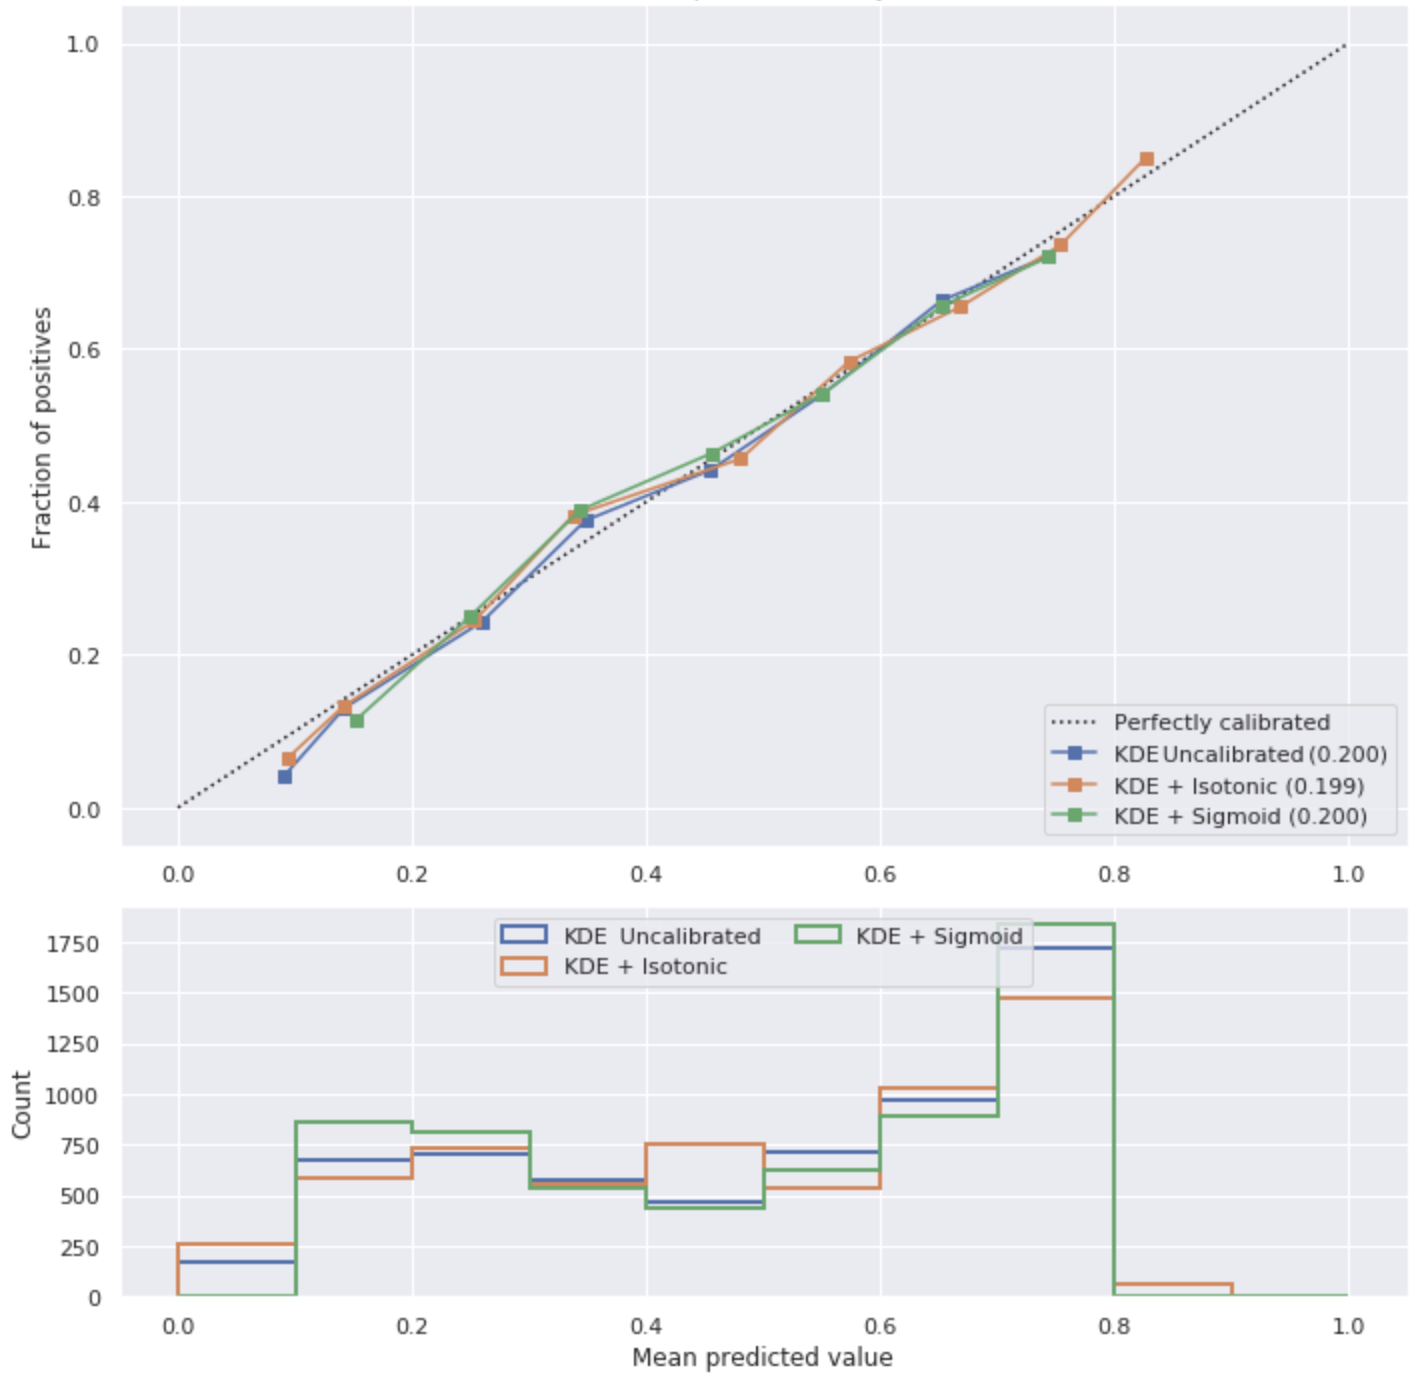
\includegraphics[width=1.0\linewidth]{images/4-ml-based-predictor/calibration2.png}
\caption{Reliability curve (top) for the KDE-based classifier predictions on Pixel barrel hit-pairs with $ w_{\eta} \leq 0.4$mm. Comparison of the uncalibrated KDE-based classifier with calibrated classifiers applied to the same training and test dataset. Common calibration techniques (Isotonic and Sigmoid functions) were tested. Models are evaluated based on their mean squared error, known as the Brier score quoted in the legend. The count for each distribution is also shown (bottom) as a function of mean predicted value.}
\label{fig:calibration}
\end{figure}


\subsection{Predictions and Evaluation}

Figure \ref{fig:predictions-pb-2d} shows the adjusted classifier predictions for Pixel barrel hit-pairs after using the probability thresholds obtained from the corresponding ROC curves. A 2-dimensional acceptance-rejection region is observed; the black region of acceptance shows hit-pairs predicted with correct hit association. This follows a somewhat \textit{linear corridor} trend with a moving average as $w_{\eta}$ increases. Regions of hit-pair rejection are shown in red and fall into two main categories; the first are predicted to have low $w_{\eta}$ and large track inclination, the second predicted to have large $w_{\eta}$ and small track inclination. Overall, the recall achieved for hit-pairs with correct hit association was determined to be a tuned 95\%. Other metrics typically used within machine learning problems to evaluate the performance of classification models are the precision and F1 score defined as:


\begin{equation}
    Precision = \frac{TP}{TP + FP}, \quad F1 = \frac{2 \times precision \times recall}{precision + recall}
\end{equation}

where FP (False Positive) indicates the number of truth 0 hit-pairs incorrectly classified by the model and the recall is also known as the TPR. The precision refers to the the quality of the positive prediction made by the model, defined as the number of true positives divided by the total number of positive predictions. In other words, the precision provides the fraction of relevant instances among the retrieved instances. The F1 score combines the precision and recall into a harmonic mean. The precision achieved was 56\% and the F1 score achieved was 71\%. Typically, within ML algorithms one wants to optimize for either precision or recall, or find a balance between them. However, there is usually a trade-off between the two. In this study, there is greater importance in optimizing for the recall as this will allow for the prediction of FNs, and hence fakes, to be low.

% This is expected to originate from the forward region of the detector and....

For each classifier, the triplet selection efficiency and total seed rejection efficiency were evaluated, shown in Figure \ref{fig:predictions-pixel-barrel-and-triplet-efficiencies}. The seed selection efficiency is defined as the proportion of seeds with both its constituent doublets classified as correctly associated, out of all correctly associated seeds corresponding to MC truth from ATLAS tracking algorithms. This provides an indication of recall. The total seed rejection efficiency considers the proportion of rejected seeds, thereby providing an estimate of the total CPU time saved. This triplet validation stage provides an indication of the level of performance of the ML-based predictor directly on the seed building stage of the HLT tracking algorithm. The lower efficiency and corresponding reduced purity at $w_{\eta} \sim$ 2.0 mm is due to the transition between the barrel and endcap Pixel detector layers. Overall, the seed selection efficiency achieved was 74.8 $\pm$ 0.1\% and the total seed rejection efficiency was 41.5 $\pm$ 0.1\%. This is primarily dominated by the low cluster width distribution ($w_{\eta} \leq$ 0.4 mm) where the greatest statistics is available for training data.


%The seed selection efficiency is defined as the proportion of seeds with both its constituent doublet pairs classified as correctly associated, out of all correctly associated seeds corresponding to MC truth from ATLAS tracking algorithms. and the total seed rejection efficiency considers the proportion of rejected seeds, thereby providing an estimate of the total CPU time saved. The lower efficiency and corresponding reduced purity around ��! ~ 2.0 mm is due to the transition between the barrel and endcap pixel detector. Errors shown here are purely statistical.


\begin{figure}[htbp!] 
    \centering
    \subfloat[]{%
        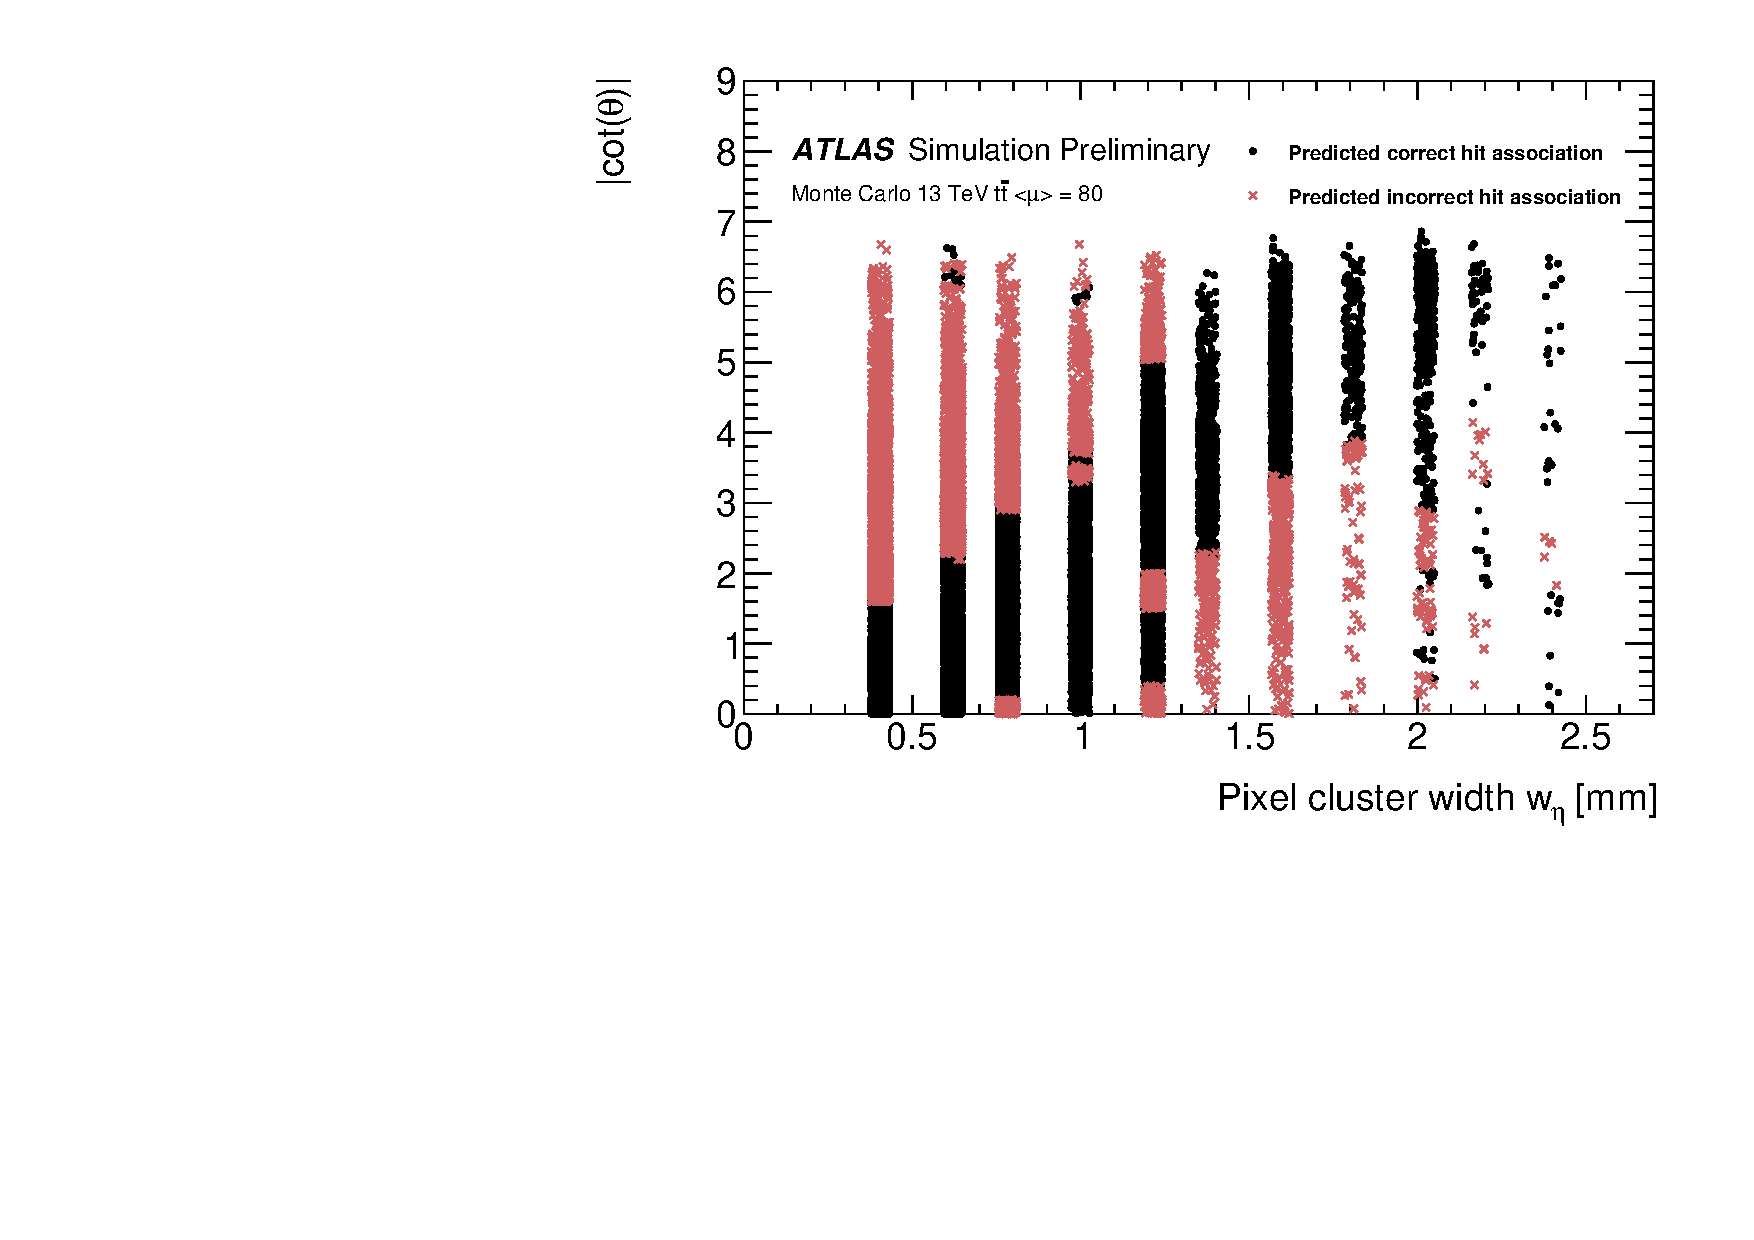
\includegraphics[width=0.98\textwidth]{images/4-ml-based-predictor/scatter_kde_predictions.pdf}%
        \label{fig:predictions-pb-2d}%
        }%
    \hfill%
    \subfloat[]{%
        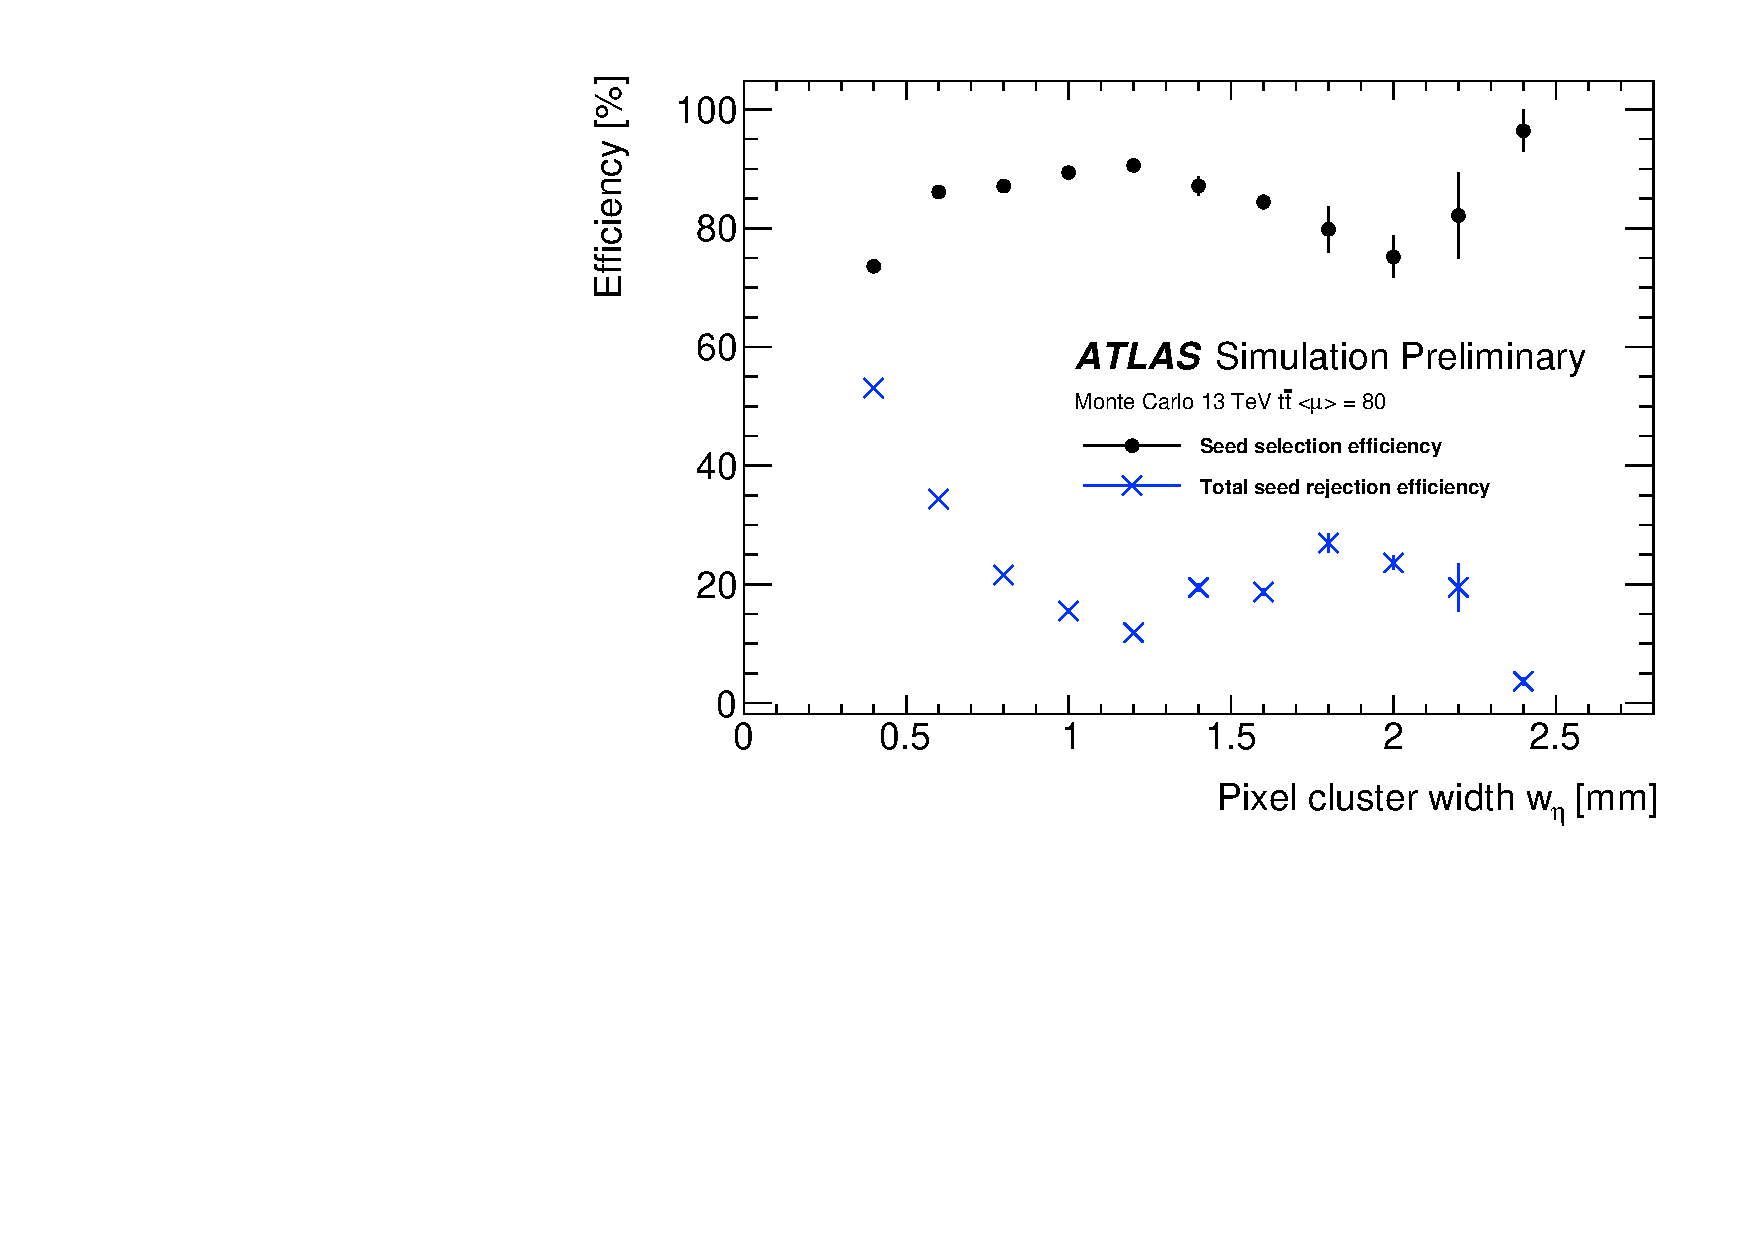
\includegraphics[width=0.98\textwidth]{images/4-ml-based-predictor/triplet_eff_metrics.pdf}%
        \label{fig:predictions-pixel-barrel-and-triplet-efficiencies}%
        }%
    \caption{(a) Predicted classification of Pixel barrel hit pairs from the ATLAS Pixel detector, trained using a set of ML classifiers to distinguish hit pairs matched to tracks corresponding to truth particles. Hit pair features used in training: $\lvert \cot(\theta) \rvert$, where $\theta$ is the inclination angle of the hit pair to the z-axis and the Pixel cluster width $w_{\eta}$. The corresponding seed selection efficiency and total rejection efficiency are shown in (b). Errors shown here are purely statistical.}
\end{figure}





\section{Application of Hit-Pair Predictor}
\label{application-of-hit-pair-predictor}

\subsection{Look-Up Table Generation}
\label{LUT-generation}

Classifier predictions for the Pixel regions were implemented directly into the ATLAS HLT \texttt{Fast Tracking} algorithm in the form of a Look-Up Table (LUT). This was achieved by first smoothing classifier predictions using Morphological filtering \cite{morphological-filtering} and then converting the acceptance region into a table. With reference to Figure \ref{fig:predictions-pb-2d} the predictions from classifiers $w_{\eta} > 2.0$ mm were not included in the morphological filtering, due to the low volume of statistics in this region. 

Morphological filtering is an image processing technique whereby non-linear transformations are applied to the binary matrix of an image, altering the features. Such non-linear operations include \texttt{dilation} and \texttt{erosion}. Dilation enlarges bright regions and shrinks dark regions, whereas erosion does the inverse of this. A combination of dilation and erosion was applied to the predictions made by the KDE-based classifiers for both the Pixel barrel and endcap via rectangular structuring elements to achieve a smoothed structure. This was done in order to encourage horizontal extrapolation and elongation of the acceptance region.

The resulting acceptance region was converted into a binned LUT, the $w_{\eta}$ axes was divided into 45 bins between 0.0 - 3.0 mm and the $\lvert \cot(\theta) \rvert$ axes divided into 30 bins between 0.0 - 9.0, and the region to accept was recorded in the LUT. The bin values were chosen based on a heuristic choice, where the granularity of the acceptance region can be made stricter or looser depending upon the requirements and the degree of morphological filtering. A predefined LUT is a much more computationally efficient procedure than predicting class labels using a trained model. The LUT is fed directly into the \texttt{Fast Tracking} trigger algorithm, providing fast look-up to reduce computational overheads and the table itself is a very low cost option in terms of storage requirements. 



% \subsubsection{ML Filtering Modes}




\subsection{Performance Evaluation}
%DONE

The track reconstruction efficiency as a function of MC truth track $\eta$ and $p_T$ for the \texttt{Fast tracking} trigger stage are shown in Figure \ref{fig:efficiencies-ml-hit-pair-predictor}. The standard track seeding approach is compared with the application of ML filtering within the Pixel detector. The standard seeding achieved an average tracking efficiency of 95\% with respect to MC truth tracks. The application of ML filtering at $\langle \mu \rangle$ = 80, achieved an average tracking efficiency of 93.9\%. The main loss in efficiency is observed at large $\lvert \eta \rvert$, due to the transition between the barrel and endcap Pixel detector. This can be improved by generating greater statistics in this region within classifier training. Overall, there is little deviation in track reconstruction efficiency from the standard trigger seeding with application of ML extensions. In addition, there is an asymmetric nature in the efficiency as a function of $\eta$ observed in both the standard track seeding and track seeding with ML filtering in Figure \ref{fig:efficiencies-ml-hit-pair-predictor-eta}. One would expect a symmetric distribution due to the detector geometry. However, this is due to the alignment of the pixel modules being slightly rotated with respect to the z-axis. This type of geometry can precisely create this asymmetric effect.



\begin{figure}[htbp!] 
    \centering
    \subfloat[Efficiency vs. MC truth track $\eta$]{%
        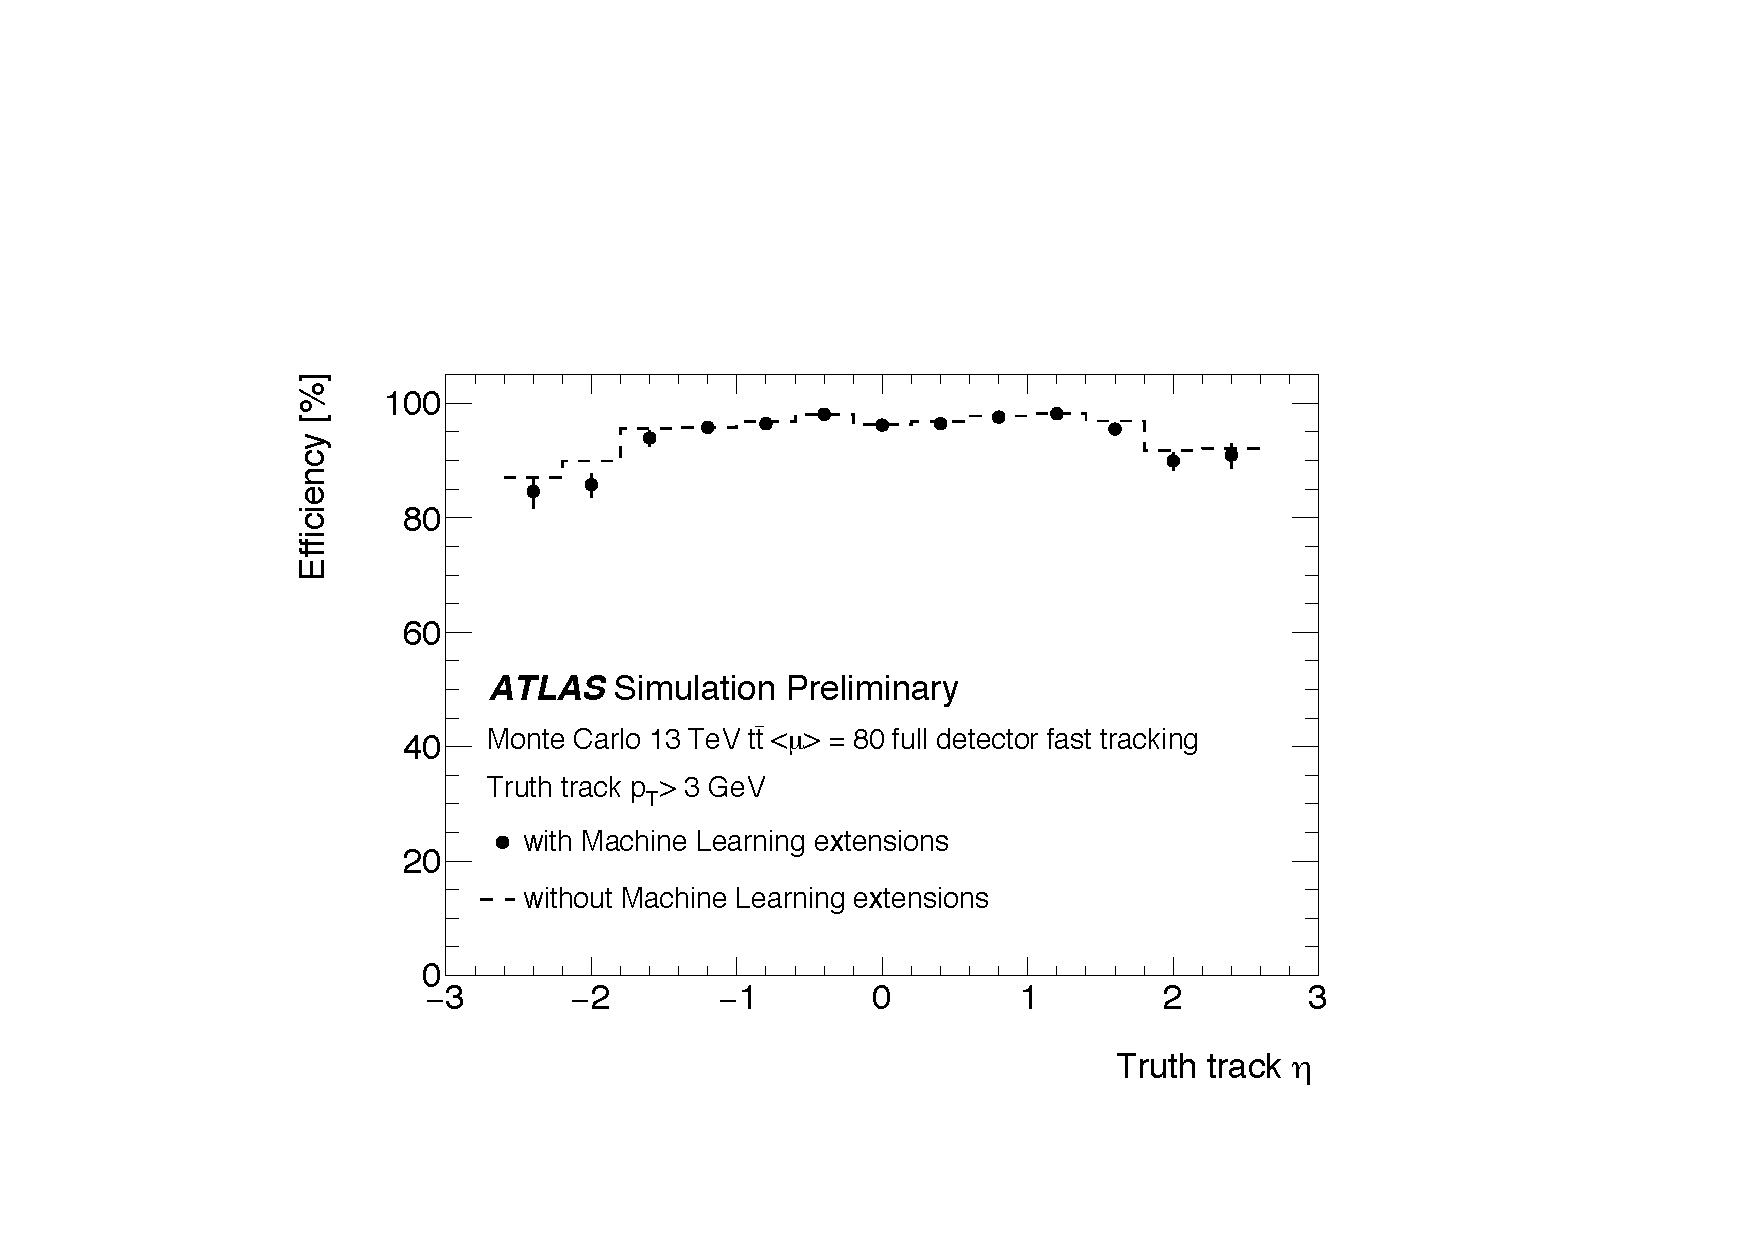
\includegraphics[width=0.92\textwidth]{images/4-ml-based-predictor/efficiency_eta.pdf}%
        \label{fig:efficiencies-ml-hit-pair-predictor-eta}%
        }%
    \hfill%
    \subfloat[Efficiency vs. MC truth track $p_{\mathrm{T}}$]{%
        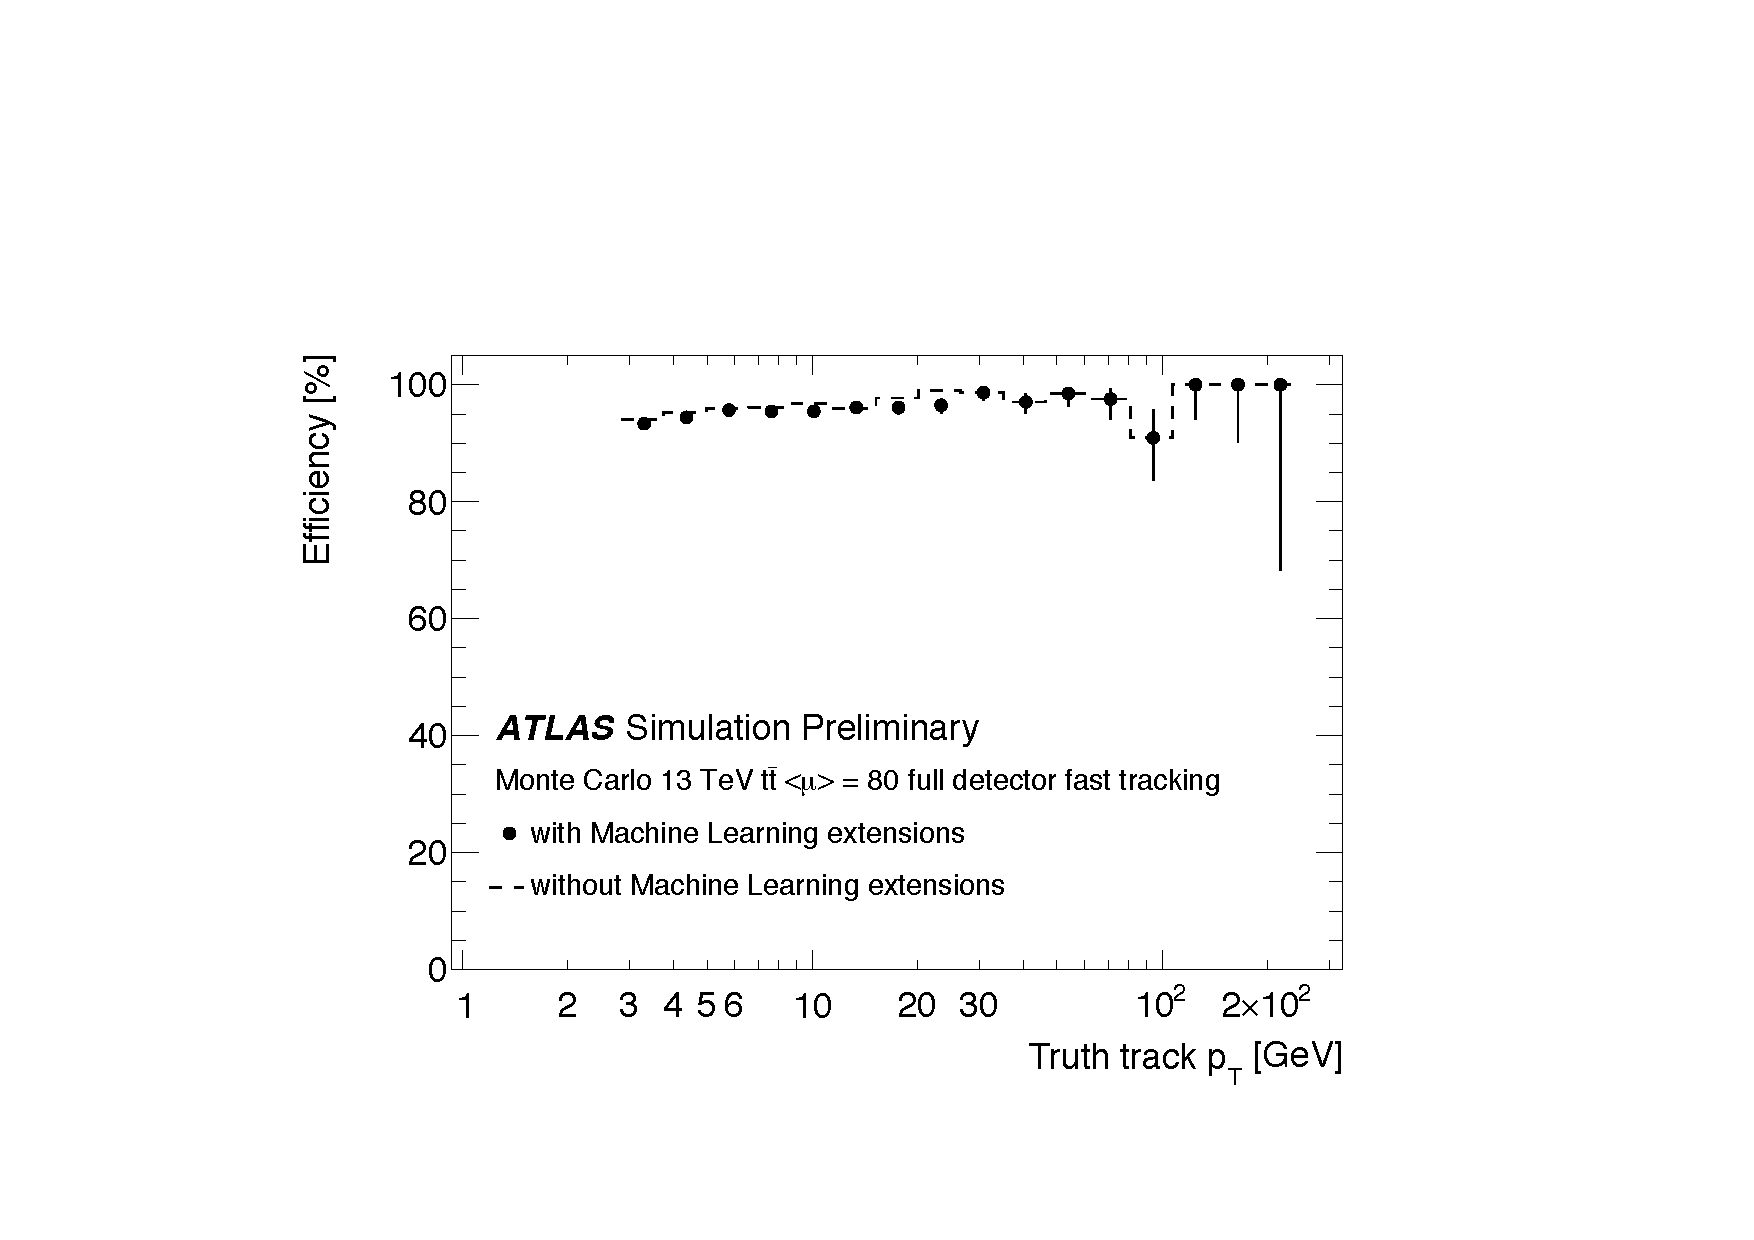
\includegraphics[width=0.92\textwidth]{images/4-ml-based-predictor/efficiency_pT.pdf}%
        \label{fig:efficiencies-ml-hit-pair-predictor-pt}%
        }%
    \caption{Tracking efficiencies as a function of track parameters, for $p_{T}$ > 3 GeV for the ATLAS full detector tracking with $t\overline{t}$ Monte Carlo 13 TeV and mean pile-up interaction multiplicity of $\langle \mu \rangle$ = 80. The data points show the efficiency when using machine learning extensions in the seed building stages of the fast tracking trigger in the ATLAS pixel detector, prior to the track fitting. The dashed line shows the efficiency of the standard trigger seeding with no application of machine learning extensions. The errors shown are purely statistical \cite{public-hlt}.}
    \label{fig:efficiencies-ml-hit-pair-predictor}
\end{figure}




\subsubsection{CPU Time Comparison}
% DONE

% TODO: know how the speed-up factor was measured - within an isolated testbed environment, with as little other processes occuring at the same time. Measuring the fastest time, and hence the greatest speed-up factor, not the average! - this is important here

Table \ref{tab:cpu} summarises the breakdown in speed-up factors achieved at various stages within the \texttt{Fast Tracking} trigger algorithm, with the application of the trained LUT for the Pixel region. The total speed-up factor achieved in the full detector with application of ML extensions at $\langle \mu \rangle$ = 80 was observed to be 2.3. The greatest saving in CPU time is achieved during the \texttt{Seed Processing} stage, as a direct result of the significant reduction in the number of seeds. The average number of seeds processed for the standard tracking is $O(10^{4})$, whereas with the introduction of ML filtering for pixel seeds, approximately 78\% fewer seeds were selected for further processing. This significant reduction in CPU time does not only benefit the \texttt{Seed Processing} stage of the combinatorial track following algorithm in ATLAS, but also propagates to the \texttt{Track Fitting} stage.

\begin{table}[!htbp]
\caption{Performance of the ATLAS full detector tracking with MC 13 TeV $t\bar{t}$ samples at $<\mu> = 80$, with the application of ML extensions for filtering on pixel detector hit-pairs in the \texttt{Fast Tracking} trigger stage \cite{public-hlt}. The total speed-up factor and breakdown of speed-ups at different stages of the \texttt{Fast Tracking} trigger algorithm are presented, each speed-up is presented with respect to the standard trigger seeding where no ML extensions are applied.}
\begin{center}
\begin{tabular}{llll}
\toprule
Total Speed-up Factor & Seed Generation & Seed Processing & Track Fitting \\
\hline
2.3 & 1.3 & 3.3 & 1.5 \\ 
\bottomrule
\end{tabular}
\end{center}
\label{tab:cpu}
\end{table}

\subsubsection{Changing Pile-up Conditions}
% DONE

Table \ref{tab:pileup} summarises the relative efficiency loss and relative speed-up factor, with application of ML extensions for the ATLAS pixel detector for various $<\mu>$, presented with respect to the standard trigger seeding, where no ML extensions were applied. A general trend is observed whereby the speed-up factor increases as $<\mu>$. At $<\mu>$ = 80, the loss in track reconstruction efficiency was observed to be 1.1\%, which was acceptable by the ID trigger performance requirements at the time of writing.


\begin{table}[!htbp]
\caption{Performance of the ATLAS full detector tracking with MC 13 TeV $t\bar{t}$ samples at $<\mu>$ = 40, 60 and 80, with the application of ML extensions for filtering on pixel detector hit-pairs in the \texttt{Fast Tracking} trigger stage\cite{public-hlt}. The absolute loss in average tracking efficiency and the total speed-up factor for seeded track finding are presented with respect to the standard trigger seeding where no ML extensions were applied. The efficiency loss is mainly observed at large $|\eta|$. The statistical uncertainties in efficiencies are $O(10^{-3})$, hence are not quoted.}
\begin{center}
\begin{tabular}{ccc}
\toprule
$<\mu>$ & Efficiency Loss (\%) & Total Speed-up Factor  \\
\hline
40 & 0.7 & 1.6 \\
60 & 0.7 & 2.1 \\
80 & 1.1 & 2.3 \\
\bottomrule
\end{tabular}
\end{center}
\label{tab:pileup}
\end{table}


\section{Other Approaches}
\subsection{Multiple Acceptance Regions}
% DONE

When training on varying permutations of train and test data sets, a second acceptance region was frequently predicted for the 1-dimensional distributions where Pixel barrel hit-pairs possess low cluster width and high track inclination. This second region is highlighted in Figure \ref{fig:multiple-acceptance} which shows the KDE-based classifier's predictions for a particular train-test permutation. The hit-pairs predicted as belonging to class 1 having correct hit association for $w_{\eta} = 0.6$mm and $w_{\eta} = 1.0$mm appear at the tail ends of these distributions. These hits were isolated and their local cluster position in the $\eta$ direction was analysed. Approximately 60\% of hits possessed the largest absolute local cluster position and this was observed for each occurrence of a second acceptance region appearing at low cluster-width and high track inclination. This corresponds to hits being located at the extremes of the barrel module, since their dimensions are approximately 20mm $\times$ 60mm \cite{pixel-module-dimensions} and strongly suggests that the second acceptance region had originated from module edge Pixels. Further investigation would be needed in order to handle these spacepoints separately. One reason for separate handling of these spacepoints is that morphological smoothing is applied uniformly to an image, hence any dilation may interact with the general shape of the main acceptance region and would increase the proportion of fakes accepted.

\begin{figure}[!htbp]
% \begin{figure}[htbp]
\centering
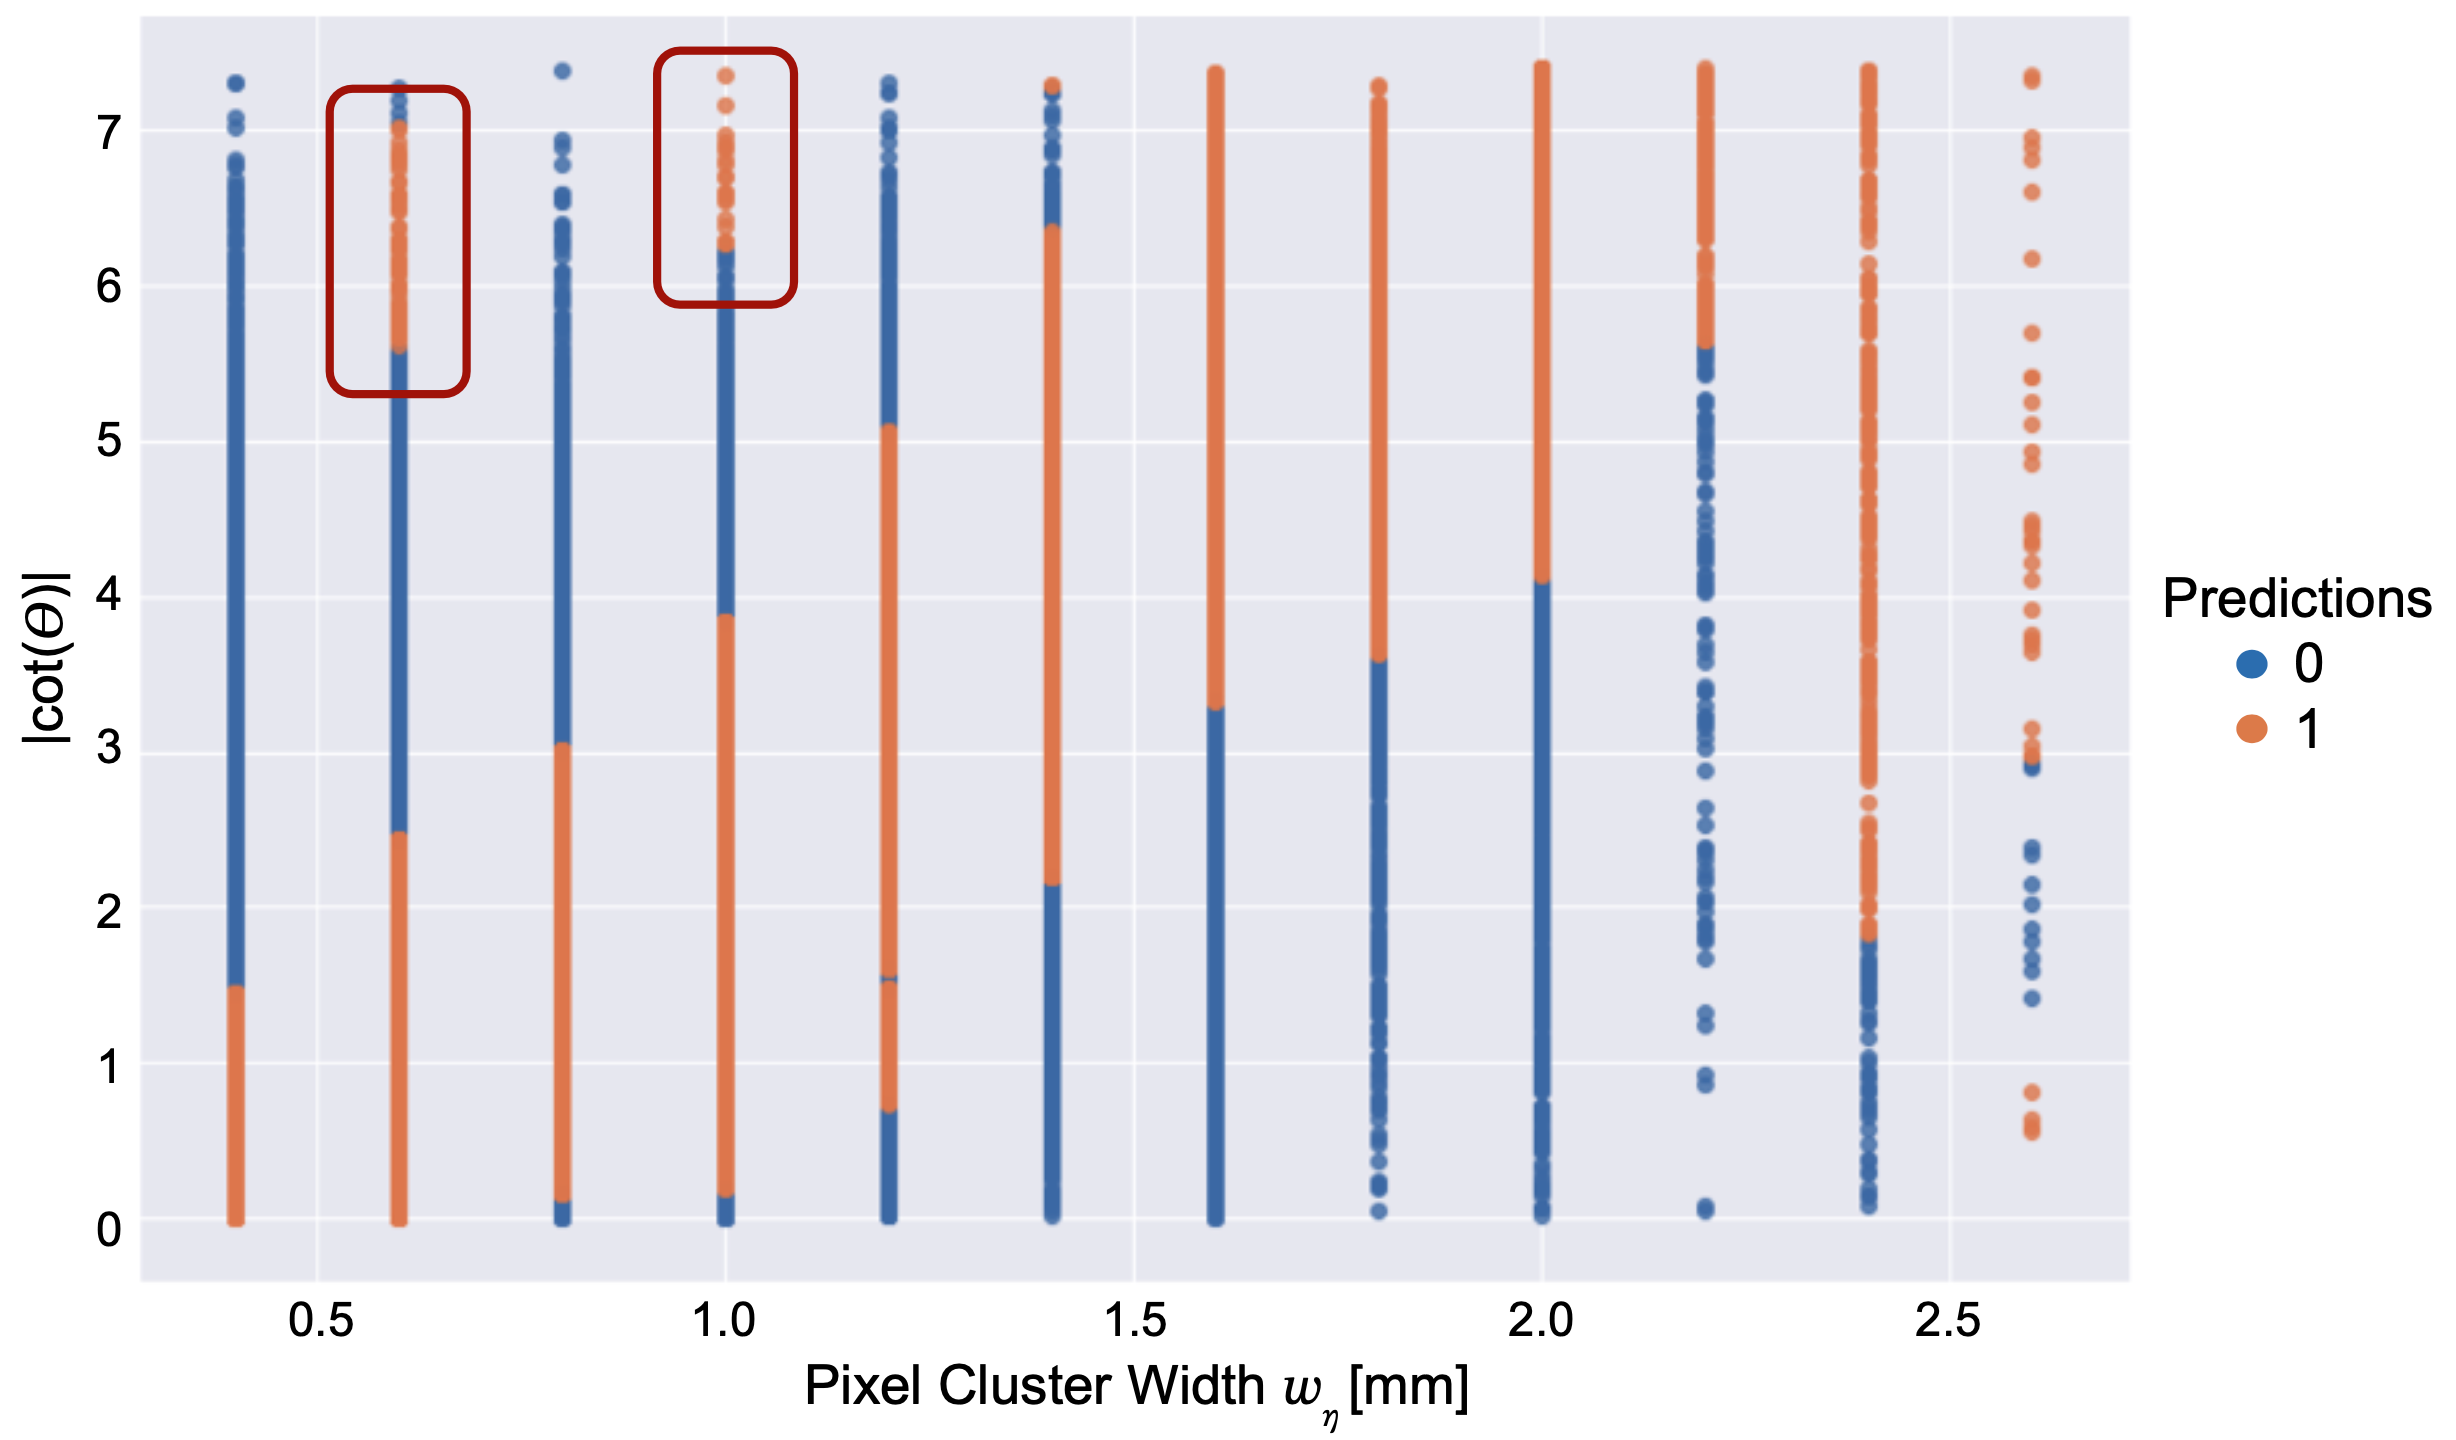
\includegraphics[width=0.98\linewidth]{images/4-ml-based-predictor/Multiple_acceptance_regions.png}
\caption{KDE-based classifier predictions for the Pixel barrel hit pairs. Multiple acceptance regions are observed at large track inclination for $w_{\eta} = 0.6$mm and $w_{\eta} = 1.0$mm, circled in red.}
\label{fig:multiple-acceptance}
\end{figure}


\subsection{Support Vector Machine}
% DONE

% See this website for further explanation 
% https://towardsdatascience.com/support-vector-machine-introduction-to-machine-learning-algorithms-934a444fca47
% multi class classification: one-to-rest
% https://towardsdatascience.com/multiclass-classification-with-support-vector-machines-svm-kernel-trick-kernel-functions-f9d5377d6f02

Another supervised learning algorithm investigated was the Support Vector Machine (SVM) \cite{svm}. The objective of a SVM is to find a hyperplane (known as a decision boundary) in a N-dimensional space (where N is the number of features) that distinctly classifies the data points and is typically used in binary classification. The optimal decision boundary is one which maximizes the margins between the two classes. This provides some reinforcement that unseen data points can be classified with more confidence. For non-linear decision boundaries, the SVM uses the so-called \textit{kernel trick} to project the data into a higher dimensional space to find a plane where the data is linearly separable. 

The SVM was applied to the data in the phase space of  [$|\cot(\theta)|$, $w_{\eta}$]. However in this instance the observed discrete nature affected the mechanics of the classifier and its ability to determine a decision boundary. Therefore, a prior step to training the SVM was to apply Principal Component Analysis (PCA). PCA is commonly used as a dimensionality reduction technique \cite{pca}, however here it was applied to remove the ordinal nature of the cluster widths which introduces a systematic bias to the SVM kernel. By doing so, the data was transformed into a continuous 2-dimensional phase space, where the variance of the truth 1 class is maximal along the first principal component axis. A hyperparameter sweep of various kernels was executed using cross-validation and the polynomial kernel of third degree with hyperparameters $C=0.75$ and $\gamma=0.05$, was found to produce the highest TPR of 95\%. Hyperparameter $C$ is a regularization parameter, such that a greater $C$ would result in a smaller margin being accepted. This essentially behaves as a penalty term and controls the cost of misclassification. Hyperparameter $\gamma$ controls the distance of influence of a single training point. The predictions of the PCA-SVM classifier on Pixel barrel data and the corresponding decision boundary are shown in Figure \ref{fig:barrel-svm-pca}. The shaded orange-red region indicates predicted hit-pairs with correct association, whereas the shaded blue region indicates predicted hit-pairs with incorrect association.

By applying a combination of PCA and SVM, the classifier was able to separate the two classes well. However, the corresponding FPR obtained was 82\% and the ROC AUC was 0.53, very similar to the no-skill classifier. Both of these metrics indicate that a large proportion of hit-pairs were incorrectly accepted by the model and hence this would increase the proportion of fake seeds constructed by downstream algorithms.

% \begin{figure}[!htbp]
\begin{figure}[htbp]
\centering
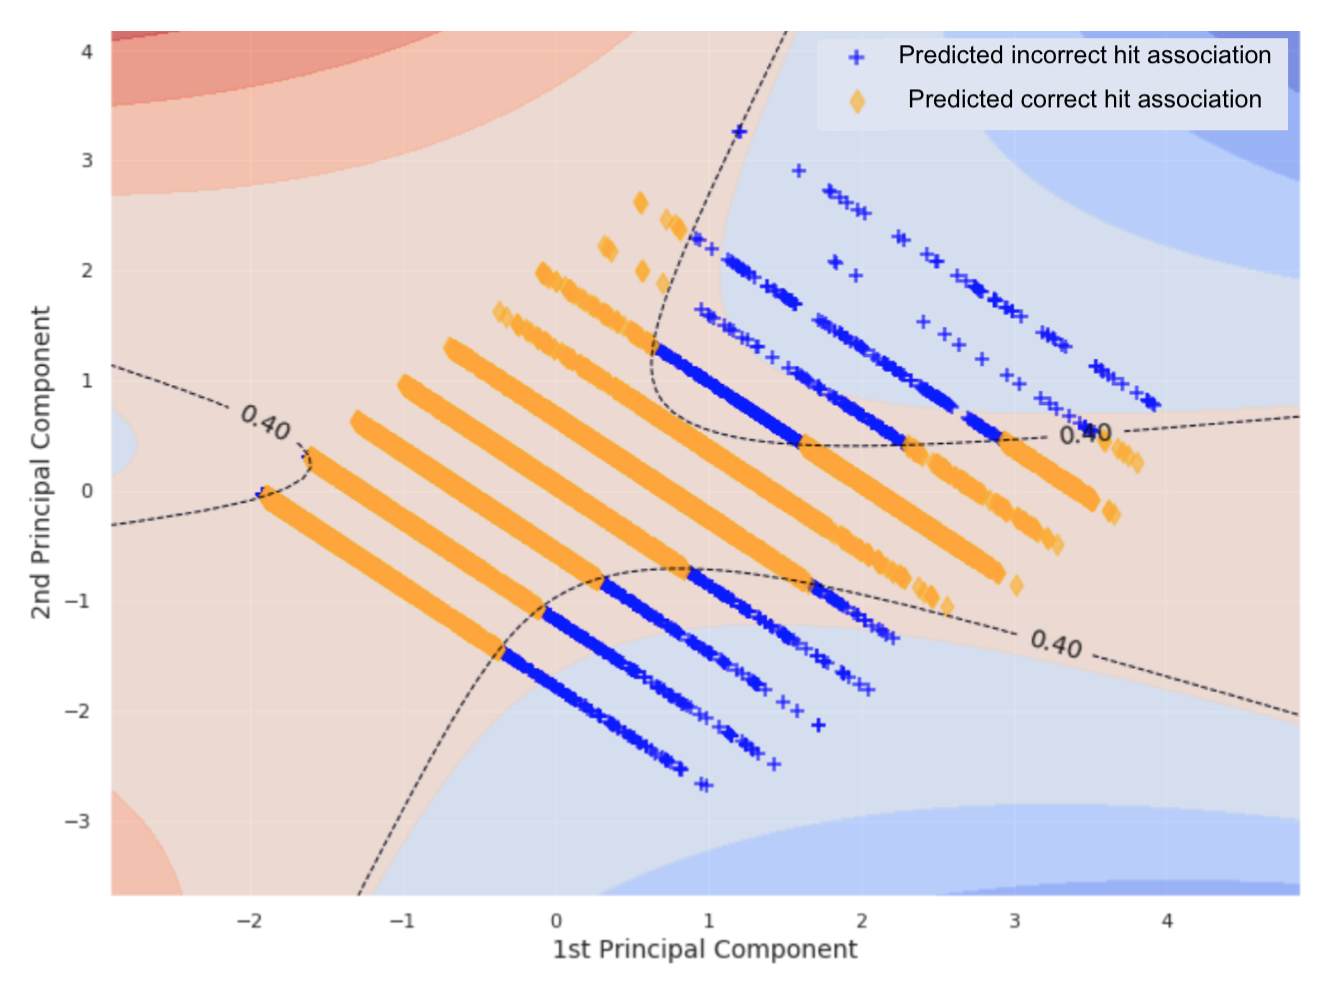
\includegraphics[width=1.0\linewidth]{images/4-ml-based-predictor/barrel-svm-pca.png}
\caption{PCA transform and SVM classifier applied to Pixel barrel hit pairs. The SVM decision boundary predictions are illustrated, where the black dotted line represents the threshold value of 0.40 yielding a TPR of 95\%. Predicted hit-pairs with correct association are illustrated by diamonds (orange) and predicted hit pairs with incorrect association are illustrated with + (blue). The SVM kernel used for the classifier was a polynomial degree 3 kernel with hyperparameters $C=0.75$ and $\gamma=0.05$. The 1st principal component indicates the axis of largest variance within the class with correct hit association doublet class.}
\label{fig:barrel-svm-pca}
\end{figure}

SVMs generally perform well, even when trained with imbalanced data sets. This, coupled with the fact that a distinct decision boundary could be easily extracted and converted into a LUT, would lead to less ambiguity in comparison to applying an extrapolation using morphological smoothing. However, there are key disadvantages by using a SVM rather than Bayes' theorem in this instance. The probabilistic information contained within each discrete one-dimensional distribution of $w_{\eta}$ is lost, which is an important feature when tuning each individual distribution. Additionally, the SVM typically fits a continuous function for the decision boundary and hence may not be strict enough in certain regions. This factor is important when considering the proportion of fake seeds being accepted using a LUT generated from such a decision boundary. Due to these key differences in classifiers, this method was not pursued further.


\subsection{Comparison with Deep Learning Approaches}

%algorithms share common approaches and methods

An algorithm with similar functionality to the method presented in this chapter, is that of the solution submitted to the TrackML competition known as \textit{Outrunner} \cite{Amrouche_2019}. The Outrunner algorithm uses a deep neural network model composed of multiple wide hidden layers and is trained to predict the adjacency matrix of hits, i.e. the probability of a hit-pair to be on the same track, in an all-to-all network connection scheme. This approach is an unstructured track following algorithm where the next hit is not provided by track extrapolation but directly by a hit index based on the hit pair classifier score. The proposed solution is prohibitively expensive for track candidate prediction, due to the extremely high combinatorics of hit pairs that are followed, yet the method is highly accurate. In contrast, the classical ML method presented in this chapter achieves the same result for hit-pair prediction without the need for high compute resources. The Outrunner algorithm also uses a LUT input approach of classifier predictions, as this provides the fastest inference and implementation for a realistic detector.

%The proposed approach is an unstructured track following algorithm where the next hit is not provided by track extrapolation but directly a hit index based on the hit pair classifier score. The reported prohibitive computation cost seems to indicates that much too many branches of the combinatorial tree are followed during the track following step. Some level of tuning could result in similar performance without much loss of accuracy, and may constitute an alternative the the combinatorial track finder approach. Although the proposed solution is prohibitively expensive to be used for making track candidate prediction, it is rather accurate, and further development might make it much more tractable. It should be noted that graph based neural network approaches, such as the one presented in [20] can combine the hit pair classification and the navigation of the adjacent hits.

% comparison with ExaTrkX project:
Additionally, the ML-based predictor developed in this chapter can also be compared to the graph construction method used by Exa.TrkX. The Exa.TrkX collaboration also predict compatible edge connections by a metric learning approach. This comprises a deep learning technique by training a MLP to learn Pixel cluster features, such as spacepoint position, the direction of the hit-pair and the dimensions of the module. Each node in the MLP is embedded into a N-dimensional latent space, which is a hugely CPU intensive task. The goal of this task is similar to the approach developed in this chapter, however they differ in their implementation. Deep learning is not used here, instead a Bayesian KDE-based classifier is employed. The main difference here is that within the procedure developed by Exa.TrkX, training is required each time as predictions have not been converted into a LUT, putting a large strain on computational resources. Whereas, in the methodology in this chapter proposes an alternative technique utilising traditional ML approaches which are less CPU intensive.


\section{Conclusion}
%DONE

As the luminosity and collision rate increases during future upgrades of the LHC program, novel and precise tracking methodologies, as well as efficient use of computing power will become increasingly important in the selection of physics objects. Therefore, it is essential that resource use is reduced, whilst maintaining the ability to reconstruct tracks with minimal efficiency loss. 

The work presented in this chapter demonstrates the algorithms and techniques implemented to optimise the HLT ID track seeding software for ATLAS Run-3 and beyond, in order to reduce the number of fake track seeds. The ML-based algorithm developed is used to predict if a pair of hits belong to the same track given input hit features of Pixel cluster width and inverse track inclination. It is encouraging to see that the application of the ML-based classifier for seed selection in the ATLAS ID has provided significant CPU savings on trained MC data at various pile-up levels. The trained predictor in the form of a LUT yields 2.3$\times$ speed-up with a 1.1\% loss in track reconstruction efficiency at $< \mu >$= 80, compared with the standard trigger tracking. The developed ML pipeline is advantageous for many reasons. It provides a flexible way to generate custom LUTs depending on the degree of efficiency required; the predictor can be trained to yield a desired TPR. This ML setup can be used to generate custom LUTs for different geometrical setups, isolating different requirements for the barrel and endcap regions, as well as for particular decay signatures depending on the required efficiency. It is useful to have algorithms that allow movement to different working points of efficiency vs CPU time, as this allows one to optimise the trigger depending on the requirements. The fast lookup implementation bodes well in a realistic detector setup. The handling of doublets which have their inner hit located in the barrel layer and their outer hit located in the endcap layer can be revisited to try to improve the performance in the transition region. Additionally, increasing statistics of the generation of hit-pairs would improve the accuracy in the prediction of incompatible doublets, particularly for regions with $w_{\eta} > 2$ mm. Overall, the reduction in fakes at an earlier stage in the HLT track seeding, ensures the reduction of fake seed propagation into downstream tracking stages and allows significant savings in CPU resources.

%i.e. jets, the training would need to be done again specifically for that purpose.

%. The use of different ML filtering modes applied to the triplets, can produce varying efficiencies (and speed up), where the three least redundant combinations are presented in this study. Additionally, proper training and tuning of the classifier can yield a required TPR, therefore allowing the flexibility in strictness.

%--------------------------------------------------
%	Chapter 5. GNN Pattern Recognition Algorithm
%--------------------------------------------------

\chapter{Graph Neural Network Pattern Recognition Algorithm}\label{chapter-5}

Once hit-pairs compatible with coming from a particle from a pp collision have been established, they are used to build a graph network. This chapter presents a novel pattern recognition algorithm to prune outlier connections in such a network in order to reconstruct tracks, by utilising GNN architectures. The application of the GNN is focused on the pixel detector, with the aim that the approach will serve as a sophisticated track seeding technique for pixel hits to form preliminary track candidates. If the GNN does not produce a large proportion of fake tracks, such an approach could save significant computational resources. The ultimate aim is to develop a realistic algorithm for track reconstruction that can be deployed in future high-luminosity upgrades of collider detector experiments. This research was presented at the 2022 Connecting the Dots (CTD) conference at the University of Princeton USA and at the dedicated GNN Google DeepMind mini-workshop at UCL in 2023. At the time of writing, this work was under review for publication in the Springer Journal: Computing for Software and Big Science \cite{Lad_2023_gnn}. This chapter is organised as follows; sections \ref{gnn-algorithm-overview} to \ref{gnn-track-extration} present a breakdown of the GNN algorithm and Section \ref{gnn-application-toy-model} illustrates an application on a simple toy MC model.


\section{Algorithm Overview}
\label{gnn-algorithm-overview}

In the context of GNNs, individual hits or clusters of hits are modelled as graph nodes and track segments are modelled as graph edges. Once the graph network is constructed, each edge is modelled as a Gaussian state in order to represent a partial estimate of the track parameters and hence approximate the local track state probability density. Therefore, each node is initialised with a Gaussian mixture of track states, local to its neighbourhood of connections. The GNN-based pattern recognition algorithm is formalised as an iterative mixture reduction problem. This allows the deactivation of incompatible connections (GNN edges termed as outliers), enabling the improvement of track parameter estimates and iterative extraction of track candidates as the network evolves. 

After the initialisation stage, the network evolves iteratively, where an iteration is made up of three main stages illustrated in Figure \ref{fig:flowchart}. 

\begin{figure}[htbp]
    \centering
    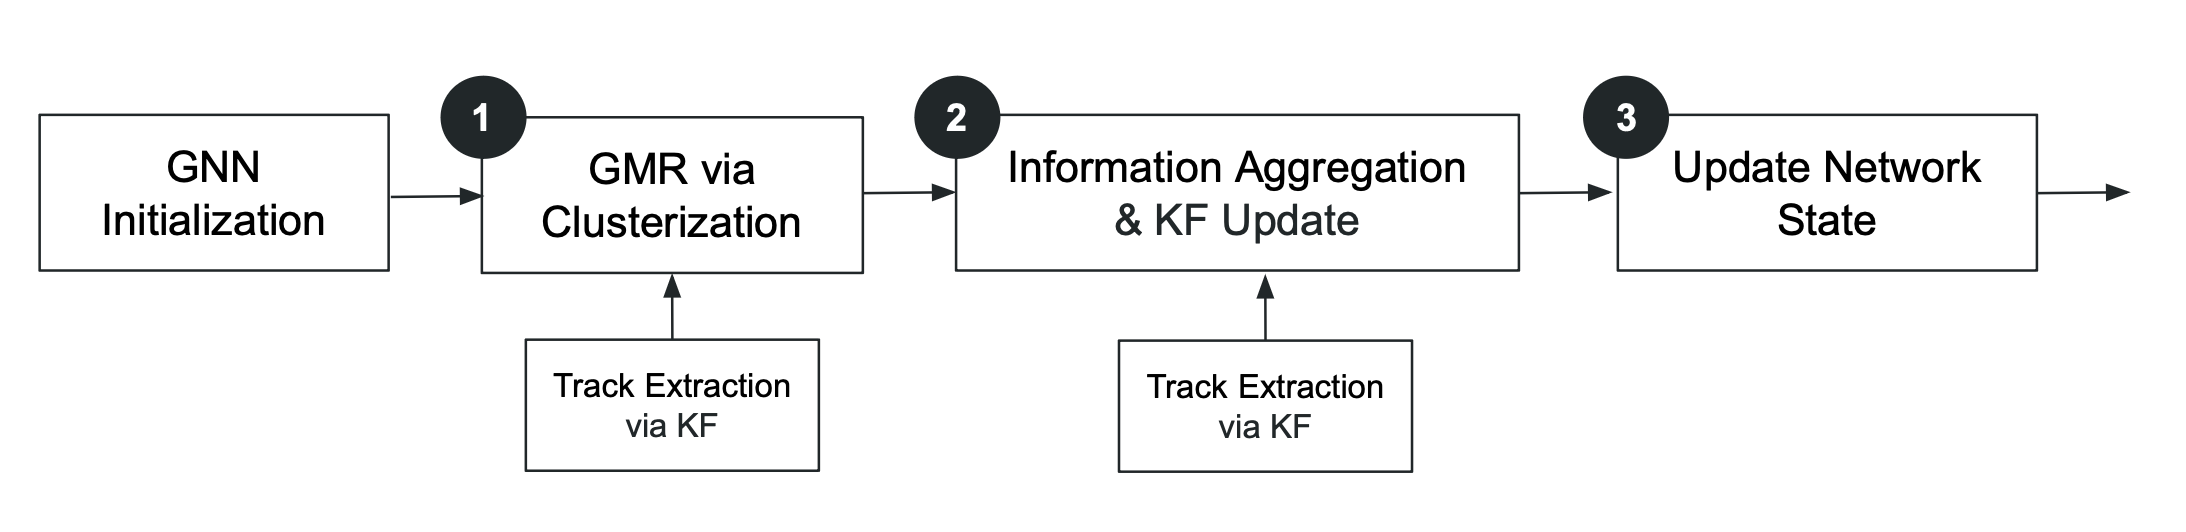
\includegraphics[width=0.98\textwidth]{images/5-gnn-algorithm/gnn-workflow.png}
    \caption{Flow chart illustrating all stages making up an iteration of the GNN-based algorithm. After each stage, a Kalman filter (KF) is applied in order to iteratively extract candidates. After stage three, a further Gaussian Mixture Reduction (GMR) stage would be applied repeating the iterations.}
    \label{fig:flowchart}%
\end{figure}


The first stage applies a Gaussian Mixture Reduction (GMR). This involves a traditional ML approach, whereby compatible Gaussian states are grouped together using clustering techniques and outlier states can be identified. Following this, an Information Aggregation stage is executed, which leverages message passing between adjacent nodes in a neighbourhood. The compatibility of neighbouring states is then assessed via extrapolation, in order to improve local track parameters. The third stage involves updating the network state at each node, with specific connections being deactivated as the network evolves. A graph splitting algorithm is also applied directly after the first two stages, in order to identify good track candidates, and if discovered they are extracted. 

Unlike traditional methodologies whereby MLPs are employed for deep learning strategies \cite{Caillou:28155782}, the proposed GNN leverages simplified KFs embedded in the network which are used for two main purposes. Firstly, the KF is embedded directly into the algorithm and used as a mechanism for information propagation during the second stage, such that the precision of track parameters can be iteratively improved. Secondly, the KF is used to apply a track fit for the extraction of compatible track candidates. This allows the algorithm to efficiently exploit a priori knowledge about charged particle dynamics as the network evolves.

The excitation and inhibition rules of individual edge connections are designed to facilitate the “simple-to-complex” approach for “hits-to-tracks” association, such that the network starts with low hit density regions of an event and gradually progresses towards more complex areas. As the network evolves, the uncertainty in local track parameters decreases until there are no more track candidates that fulfil the criteria for a good track. This is the end state of the network where isolated nodes, track fragments and unresolved ambiguities will remain.


\subsection{Model Assumptions and Key Components}
\label{chp5-model-assumptions}

The following is a summary of the main assumptions and important aspects used within the construction of GNN model. These points are further elaborated in Sections \ref{gnn-network-initialization} - \ref{gnn-application-toy-model} and are stated here for ease of reference.


\begin{itemize}
    \item Each node in the graph network represents an individual hit or clusters of closely located hits. Each edge models the relationship between the connected node-pairs in the form of a Gaussian state vector, this models the partial estimate of track parameters between a particular node-pair. 
    \item The model assumes each node represents a single truth track with a set of noisy connections. Intersecting tracks are not modelled; this would be an extension of this work.
    \item The main sources of uncertainty in track state vectors arise from the measurement error and error due to multiple scattering, assumed to be uniform.
    \item Track detection inefficiencies are random and cannot be learned, so edge connections are allowed up to two detector layers apart to compensate for cases when a track is not detected in the intermediate layer. As a result, clustering of track state vectors can occur across layers.
    \item Exchange of state information between nodes (message passing) occurs bidirectionally along \textit{active} edge connections only. 
    \item The model evaluates the compatibility of state information exchanged between nodes using the Mahalanobis distance as the statistical covariance between the two states can be incorporated.
    \item Edge weights are associated to each track state and are model parameters, unlike traditional neural network weights which are learned within training.
    \item Edge weights are updated using their priors and Gaussian likelihoods. They are also normalised by the number of layers either side of the central node, assuming the track has one hit per layer.
    \item The model assumes linear track motion in the state extrapolation, track fitting and extraction stages.

\end{itemize}



\section{Graph Network Initialization}
\label{gnn-network-initialization}

The graph network is implemented using the Python library \texttt{NetworkX} \cite{SciPyProceedings_11}. Hits from a particle event are represented as nodes and predicted hit-pairs as edge connections. Typically, track detection inefficiencies are random such that they cannot be learned. One approach to mitigating this is to allow edge connections to be built spanning up to two detector layers apart, ensuring random cases when a track is not detected in the intermediate layer. See Chapter \ref{chapter-4} for further details on the hit-pair predictor used to form edge connections. Following this, a common graph theory technique known as Connected Component Analysis (CCA), is applied using a built-in function of NetworkX \cite{networkx}. CCA detects connected regions in data structures and splits the network into smaller, more manageable, graphs referred to as \textit{subgraphs}. 

The general approach is formalised as follows. Each pairwise connection between node $i$ and neighbour node $j$ forms a Gaussian state, $X_{ij}$, representing the local track parameter estimate. Each edge has an associated prior probability $p_{ij}$ and edge weight $w_{ij}$. The prior probability of nodes $i$ and $j$ belonging to the same track is determined, assuming a track can produce at most one hit per detector layer. $w_{ij}$ is a mixture weight for the compatibility of the Gaussian state transmitted from node $i$ to neighbour node $j$, and represents the strength of the connection. The weights $w_{ij}$ are initialised uniformly and are dependent on the number of neighbours local to a node. The parameters $w_{ij}$ and $p_{ij}$ are updated as the network evolves. Note that $w_{ij}$ are not to be confused with the traditional weights associated to features within neural networks. 

For a given node $i$ and neighbour nodes $j$, a Gaussian mixture $g_i(X)$ is formed from weighted components, $\Phi_{ij}$, representing a partial estimate of track state parameters, where the general form of $g_i(X)$ is given by Eq \eqref{eqn:gaussian-mixture},


\begin{equation}
g_i(X) = \sum_{j} w_{ij}\Phi_{ij}(X, X_{ij}, C_{ij})
\label{eqn:gaussian-mixture}
\end{equation}

where $C_{ij}$ are track state covariances. All edges act as bidirectional conduits, such that message passing can occur in both directions. All edges are initialised as \textit{active}, allowing the propagation of state information between its node-pair, whereas \textit{deactivated} edges do not allow state information to be exchanged. 

%Figure \ref{fig:network-initial} illustrates a node and its neighbourhood.

% \begin{figure}[htbp]%
%     \centering
%     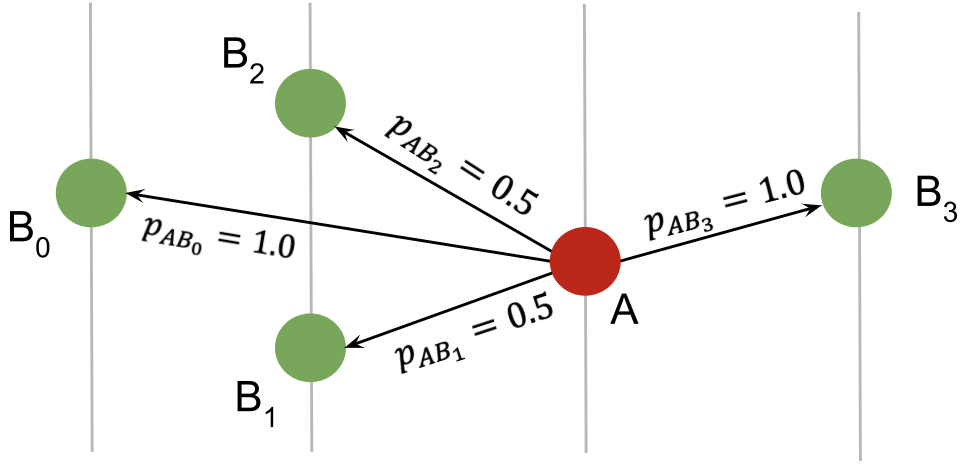
\includegraphics[width=8.8cm]{images/5-gnn-algorithm/network-initialisation.png}%
%     \caption{Prior probabilities associated to network edges of node A's local neighbourhood. Neighbours $B_j$ are located on separate detector layers shown by vertical lines. The unidirectional edges indicate the direction of propagation of state information and priors. These entities will differ from nodes $B_j$ distributing messages to their corresponding neighbourhoods.}%
%     \label{fig:network-initial}%
%\end{figure}




\section{Gaussian Mixture Reduction}
\label{section-GMR}

For nodes with a high multiplicity of edge connections, the number of potential track states can quickly rise. To make inferences within a reasonable amount of processing time, GMR is used to prevent the number of components from exploding. One computationally efficient algorithm for GMR is clustering. A high multiplicity Gaussian mixture can be approximated by one with lower multiplicity, using the traditional k-means clustering \cite{kmeans}. At each node, similar track states are grouped together forming a reduced mixture and their corresponding edges remain active, as illustrated in Figure \ref{fig:GMR-example}. By default, clustering is only applied to nodes with more than two active edge connections.


\begin{figure}[htbp!] 
    \centering
    \subfloat[]{%
        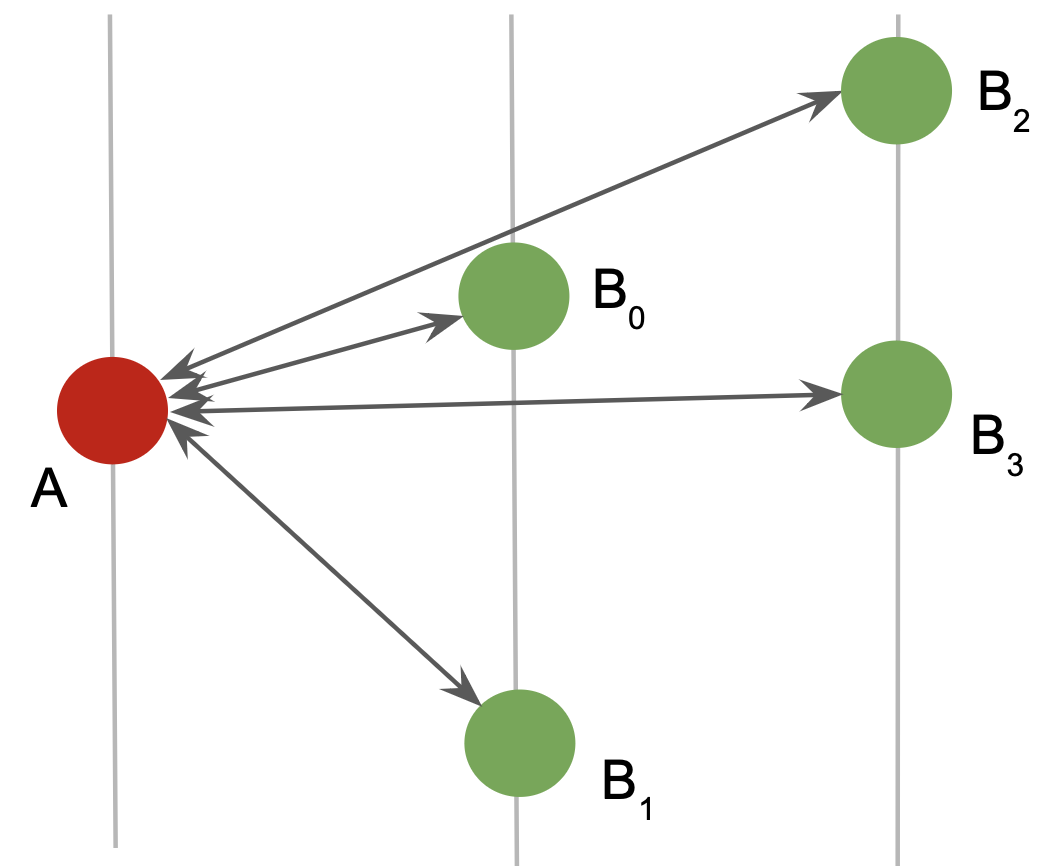
\includegraphics[width=0.42\linewidth]{images/5-gnn-algorithm/GMR-1.png}%
        \label{fig:GMR-1}%
        }%
    \hfill%
    \subfloat[]{%
        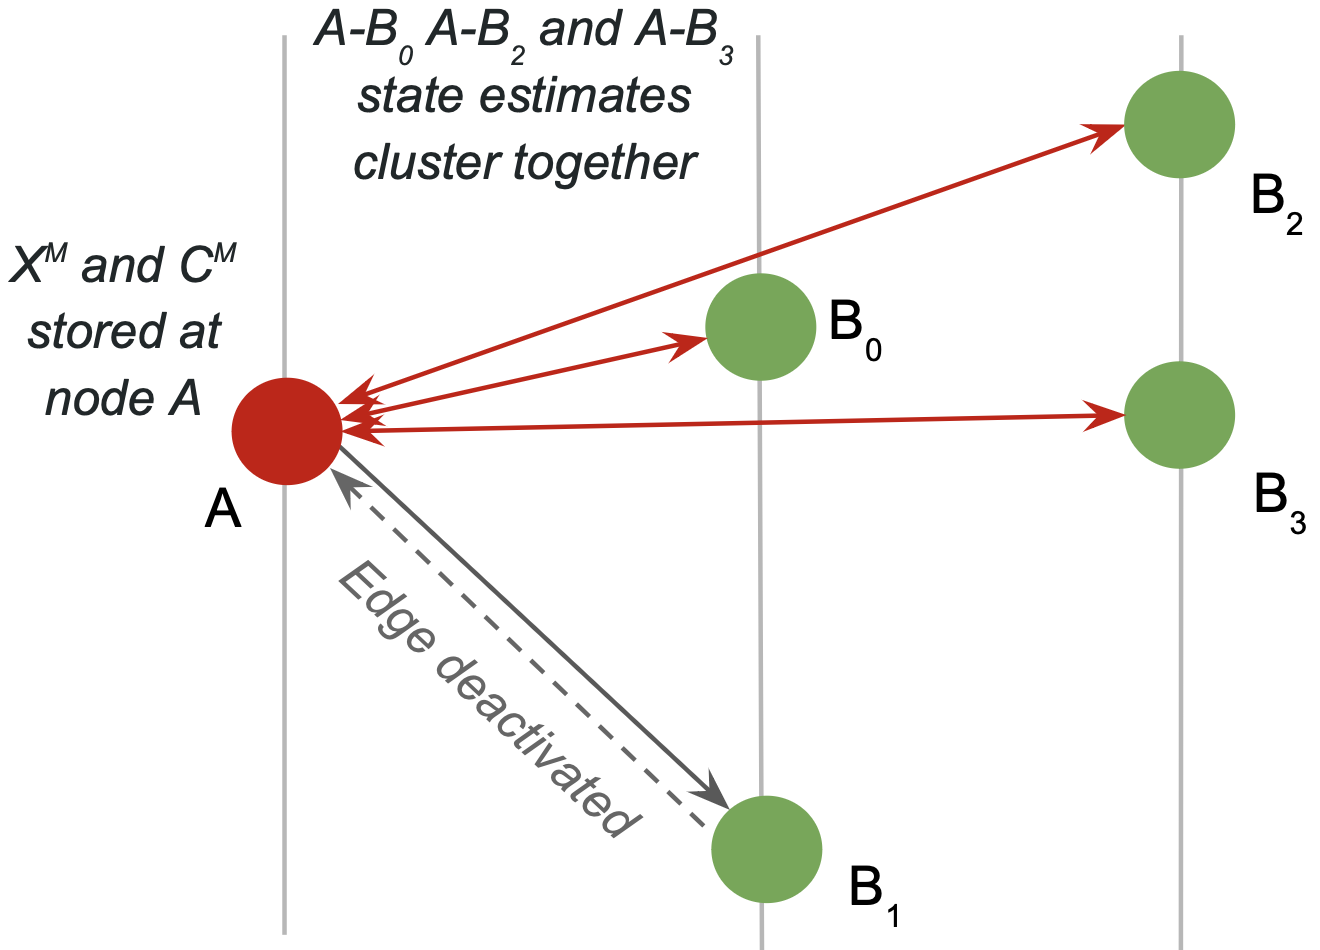
\includegraphics[width=0.57\linewidth]{images/5-gnn-algorithm/GMR-2.png}%
        \label{fig:GMR-2}%
        }%
    \caption{Illustration of GMR via clustering applied to graph networks. Independent detector layers are represented by the vertical lines.}
    \label{fig:GMR-example}
\end{figure}


Figure \ref{fig:GMR-1} shows node $A$ and its local neighbourhood $B_j$ with bidirectional edge connections. Figure \ref{fig:GMR-2} shows the expected result of GMR applied to node $A$. If clustering is successful, a merged track state estimate, $X^M$, is formed from states $X_{AB_0}$, $X_{AB_2}$, $X_{AB_3}$ clustered together and the corresponding merged state covariance, $C^M$, is formed from $C_{AB_0}$, $C_{AB_2}$, $C_{AB_3}$. Outlier states are simultaneously identified and their edges are deactivated. The incoming $B_1 - A$ edge has been deactivated (represented as a dotted line), as any incoming state information from neighbour $B_1$ is deemed incompatible at node $A$.

The merged state estimate $X^{M}$ and merged state covariance $C^{M}$ are computed using the inverse-variance weighting \cite{inverse-variance-weighting} given by Eq \eqref{eqn:inverse-variance-weighting}, where $G_{ij}$ = $C_{ij}^{-1}$.

\begin{equation}
    X^{M} = C^{M} \sum_{j} G_{ij} X_{ij},  \quad  C^{M} = \left( \sum_{j} G_{ij} \right) ^{-1}
    \label{eqn:inverse-variance-weighting}
\end{equation}

The k-means clustering is implemented using the general case of $k=1$, to model the Gaussian mixture at each node as a single track with outlier connections. For the case where a node is located in close proximity to an intersection between two tracks, two or more clusters can be expected. In such a case, the mixture reduction process is declared impossible. This part of the network remains dormant until competing edges are deactivated through information propagation from other parts of the network and the mixture becomes more unimodal. The current implementation is a limitation of k-means clustering, as the number of clusters to form at each node must be predetermined, which is a non-trivial task. An alternative procedure would include the use of DBSCAN for clustering, as no prior knowledge of the number of clusters is required as this information is determined by the clustering algorithm and would be useful in regions with intersecting tracks. However, when considering the computational complexity of such approaches, the k-means algorithm scales linearly, $O(n)$, with the number of edges $n$, compared to DBSCAN which scales non-linearly, $O(n^2)$. The work presented in this thesis is limited to the general case of k=1 case, where the extension k $>$ 1 would require further exploration. 


\subsection{The Kullback-Leibler Divergence}
In order to establish whether clustering can occur for a given node, a distance measure is used as a threshold. The Kullback-Leibler (KL) divergence \cite{KL, FRUHWIRTH19971}, $d_{KL}$, is a measure of the statistical distance between two Gaussian probability distributions and is used in the k-means algorithm to determine if track states can be grouped into a cluster. The $d_{KL}$ between $X_{ij}$ and $X_{ik}$ is given by Eq \eqref{eqn:kullback-leibler}.

\begin{equation}
    d_{KL} = tr[(C_{ij} - C_{ik})(G_{ij} - G_{ik})] + (X_{ij} - X_{ik})^{T}(G_{ij} + G_{ik})(X_{ij} - X_{ik})
    \label{eqn:kullback-leibler}
\end{equation}

The optimal $d_{KL}$ threshold will differ for each node depending on its local neighbourhood. For example, consider a node with a high empirical variance of edge orientation in its neighbour connections, $\sigma_{e}^{2}$. The corresponding $d_{KL}$ threshold will be larger in comparison to a node with a small $\sigma_{e}^{2}$, where neighbour connections are more closely orientated. To determine the optimal $d_{KL}$ threshold between pairwise $X_{ij}$ for a given node, a SVM classifier was trained against truth information using a MC simulation. See Section \ref{chapter-6-kl-threshold} for further details on the implementation.

In principal, a physical distance can also serve as an alternative measure within the clustering algorithm, such as the Euclidean distance between two neighbour nodes. However, the choice of the KL divergence is preferred over the Euclidean distance, as it is a general measure of the difference between two probability distributions. Given the underlying assumption that each edge is a partial estimate of the track parameters with corresponding mean and covariance, both of these entities are taken into account by the KL divergence, and hence reflects its statistical meaning. The KL divergence seeks to measure the correlation between variables, as it incorporates the covariance between the two measured states. In general, a state can be defined by parameters other than spatial coordinates, i.e. parameters encoded into some latent representation, therefore it is also important to consider the covariance.



\section{Information Aggregation}

\subsection{Message Passing}
Neural message passing in graph networks effectively captures the dependencies and interactions among nodes, by providing a framework to exchange information with their neighbour nodes and aggregate that information to update their own representations. Both structural information of the graph and the features associated with each node are captured.

The message passing mechanism is leveraged in the GNN algorithm in order to improve the precision of track state parameters on a local and global scale. During the previous stage (Section \ref{section-GMR}), reduced Gaussian mixtures were formed for nodes where clustering was successful. For a given node $i$, $X^M$ and $C^M$ are propagated to all neighbours $j$ which have active $i \rightarrow j$ connections. If clustering was unsuccessful for a particular node, this part of the network remains dormant until a merged state is received via message passing during later stages of the algorithm. Track state information can be propagated in both directions along active network edges. This ensures that the compatibility of received states can be validated and assessed against each node's local neighbourhood.


\subsection{Validation}
Once state information has been propagated to neighbours, the parameter estimation begins with a linear projection of the incoming track state onto the subspace of measurements. As illustrated in Figure \ref{fig:extrapolation}, for a given node $i$, each incoming $X^M$ is projected via a measurement matrix $H$, which relates the incoming track state to the measurement values. See Section \ref{gnn-application-toy-model} for implementation of matrix $H$. In order to validate if the connection between nodes $i$ and $j$ is compatible, the Mahalanobis distance \cite{mahalanobis-distance}, $\Delta \chi^{2}_{ij}$, is calculated using the residual between the projected state, $HX$, and the measurement at the neighbour node, $m$. The threshold $d_{\chi^{2}}$ is a tuned hyperparameter and represents the maximum $\Delta \chi^{2}_{ij}$ acceptable for an incoming track state. If $\Delta \chi^{2}_{ij} \leq d_{\chi^{2}}$, the connection is deemed compatible and the state can be extrapolated via a KF. If $\Delta \chi^{2}_{ij} > d_{\chi^{2}}$ then the connection is deemed incompatible and the corresponding edge is deactivated.

% \begin{figure}[htbp]
\begin{figure}[H]
        \centering
        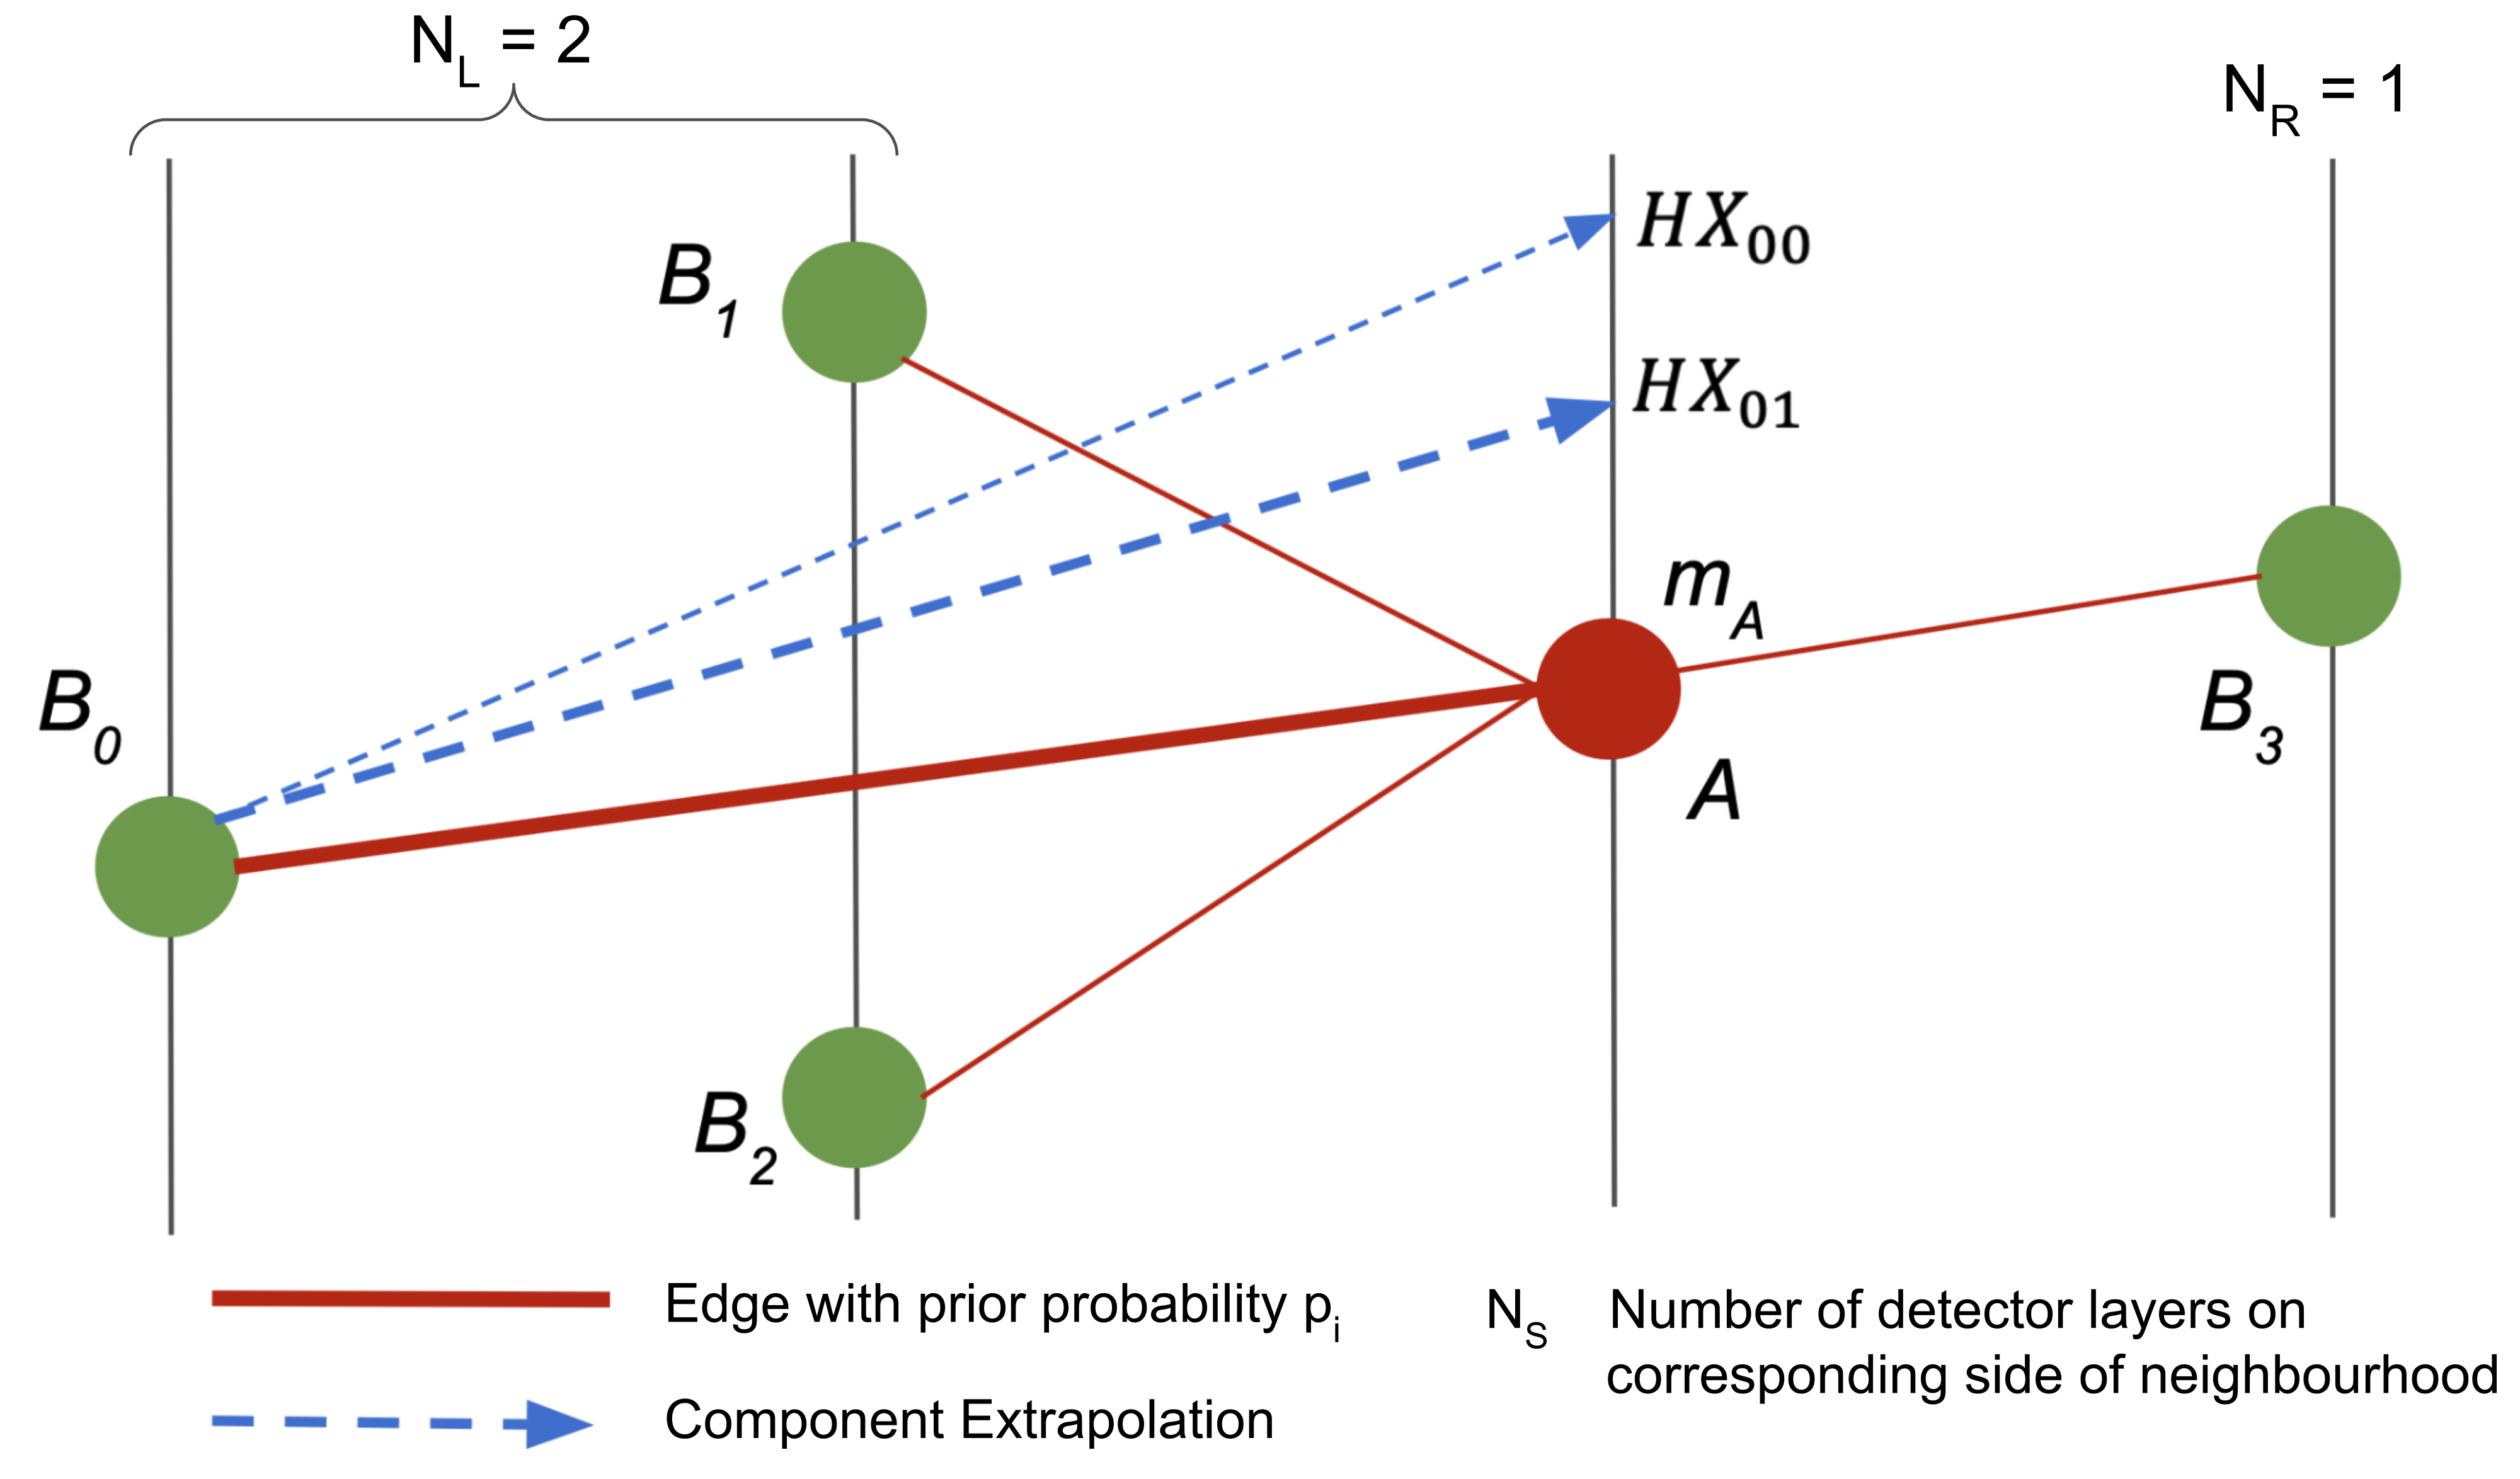
\includegraphics[width=0.95\textwidth]{images/5-gnn-algorithm/gnn-extrapolation.png}
        \caption{Illustration of track state estimates $X_{00}$ and $X_{01}$ being projected from node $B_0$ to node $A$ via a measurement matrix $H$ into the subspace of measurements. $m_A$ is the measurement at node $A$. The corresponding residual between $m_A$ and the projected incoming state from $B_0$ is used to compute the Mahalanobis distance $\Delta \chi^{2}$ to determine if the incoming state is compatible with $m_A$. $N_L$ indicates the number of detector layers on the left side of node $A$'s local neighbourhood, and $N_R$ indicates the number of detector layers on the right side, where the detector layers are represented by the vertical lines.}
        \label{fig:extrapolation}%
\end{figure}


\subsection{KF Update and Extrapolation}
\label{chapter-5-kf-extrapolation}

For compatible incoming states where $\Delta \chi^{2}_{ij} \leq d_{\chi^{2}}$, the KF update is applied in order to compute the extrapolated track state estimate, $\tilde{X}_{ij}$, and the corresponding extrapolated covariance matrix, $\widetilde{C}_{ij}$. The KF is implemented via the Python library \texttt{Filterpy} \cite{filterpy}. $\tilde{X}_{ij}$ and $\widetilde{C}_{ij}$ are given by Eqs. \eqref{eqn:extrapolation},

\begin{equation}
\tilde{X}_{ij} = F_{ij} X_{ij}^{M}, \qquad \tilde{C}_{ij} = F_{ij} \biggl( \sum C_{ij}^{M} + Q_{ij} \biggl) F^{T}_{ij}
\label{eqn:extrapolation}
\end{equation}

where $F_{ij}$ is the state transition Jacobian from node $i$ to node $j$, and $Q$ is the process noise matrix. See Section \ref{gnn-application-toy-model} for implementation of the KF update, including the transition Jacobian $F$ and process noise $Q$. 






\section{Updating Network State}
\label{gnn-updating-network-state}

As the network evolves and specific connections are deactivated, the local track parameter estimates change at each node. Therefore, the corresponding edge weights, $w_{ij}$, should reflect this for the strength of each connection, hence $w_{ij}$ are updated. Given the underlying assumption that each edge is modelled as a Gaussian probability density function, with corresponding mean and covariance, a Gaussian measurement likelihood is used to update $w_{ij}$. For the connection between nodes $i$ and $j$, the updated edge weights $\widetilde{w}_{ij}$ are computed using the normalised Gaussian measurement likelihood given by Eq \eqref{eqn:likelihood}, 

\begin{equation}
\beta_{ij} = (2 \pi \lvert S_{ij} \rvert )^{-1/2}  e^{-\Delta \chi^{2}_{ij} / 2}
\label{eqn:likelihood}
\end{equation}

where $S_{ij}$ is the joint measurement covariance matrix and $\Delta \chi^{2}_{ij}$ is the Mahalanobis distance between the projected state the measurement. The updated edge weights $\widetilde{w}_{ij}$ are given by Eq \eqref{eqn:weights}, 

\begin{equation}
\widetilde{w}_{ij} = \frac{1}{N_S} \frac{w_{ij}\beta_{ij} p_{ij}}{\sum_{k}w_{ik}\beta_{ik}}
\label{eqn:weights}
\end{equation}


where $p_{ij}$ are the prior probabilities as described in Section \ref{gnn-network-initialization}. The denominator $\sum_{k}w_{ik}\beta_{ik}$ is the summation of the product of weights and likelihoods in the neighbourhood of node $i$. The weights $\widetilde{w}_{ij}$ are divided by the number of detector layers on either side of its neighbourhood, $N_S$, in order to account for the probability that a track passing through node $i$ was detected at layer $L$. If $\widetilde{w}_{ij} < 0.1$, the corresponding edge connection is automatically deactivated as the likelihood of compatibility of this incoming track state is extremely low. This forms part of the mechanism for edge activation and deactivation. The Gaussian mixture $g_i(X)$ at each node is then composed of updated components, given by Eq \eqref{eqn:updated-gaussian-mixture}.

\begin{equation}
g_i(X) = \sum_{j} \widetilde{w}_{ij}\Phi_{ij}(X, \widetilde{X}_{ij}, \widetilde{C}_{ij})
\label{eqn:updated-gaussian-mixture}
\end{equation}

Following this update, the algorithm iterations repeat. A further GMR would follow, clustering on $\widetilde{X}_{ij}$. This allows further ambiguities to be resolved and the precision of track state parameters to be increased at each additional stage.






\section{Graph Splitting and Track Extraction}
\label{gnn-track-extration}

The design of the GNN-based framework is such that it is possible to iteratively discover track candidates after each stage. As shown in Figure \ref{fig:flowchart}, a track extraction algorithm is executed after the GMR and Information Aggregation stages.

Initially, the graph network must be split into smaller components, taking into account only edges which remain active. A CCA is applied to the network by using the NetworkX built-in function \texttt{weakly\_connected\_components}. This ensures that smaller, more manageable subgraphs are separated from the main network.

The criteria that a subgraph must satisfy in order to be considered for track extraction are as follows. Subgraphs must contain a minimum number of four nodes within the volume of interest. There must exist only one node per detector layer, so that there are no intersecting tracks or holes within the track candidate. 

If the above criteria are met, a KF is then applied in order to perform a final track fit. As opposed to applying the KF on one track segment between two nodes, similar to the method used in Section \ref{chapter-5-kf-extrapolation} for state extrapolation, the KF for track fitting considers the whole chain of track segments. Here, the filter iteratively predicts and updates track state parameters as it receives measurements from each subsequent node in the subgraph. The KF is initialised with a filter state estimate, $\hat{x}$, a filter state covariance, $\hat{P}$, state transition Jacobian, $\hat{F}$, measurement function, $\hat{H}$, measurement noise $\hat{R}$ and process noise, $\hat{Q}$.

In order to assess the quality of the track fit the p-value is computed from the $\chi^2$ statistic. The p-value obtained must be greater than 0.01. Subgraphs that fulfill all conditions are defined as good track candidates and are extracted from the network, such that their corresponding nodes and edges are removed. Subgraphs that do not meet the above criteria for track extraction, remain in the graph network for further processing.





\section{Application on a Simple MC Model}
\label{gnn-application-toy-model}

A linear 2-dimensional MC model was used to simulate seven truth tracks in the $x$-$y$ plane, each with ten hits as shown in Figure \ref{fig:ground-truth}. 

\begin{figure}[htb]
    \centering
    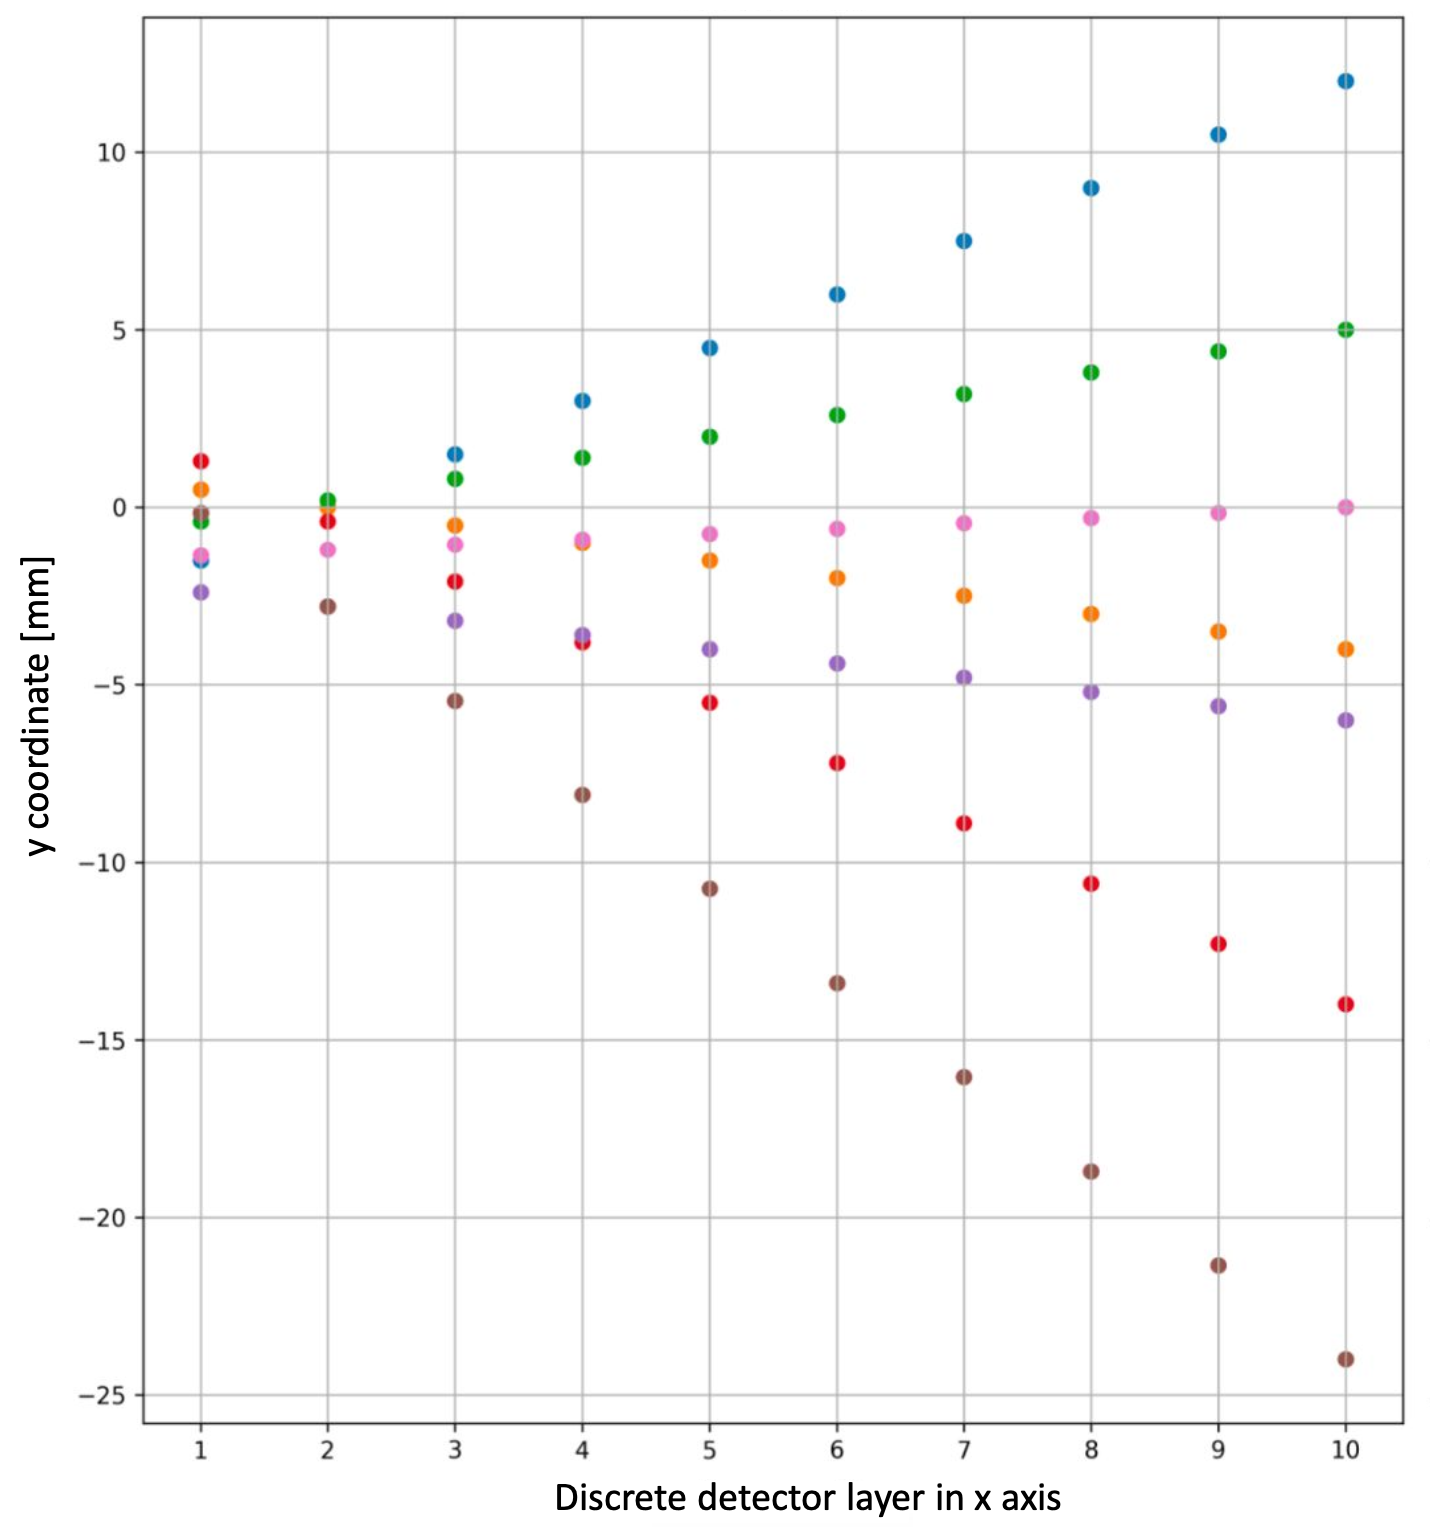
\includegraphics[width=0.78\textwidth]{images/5-gnn-algorithm/ground-truth.png}
    \caption{Simulation of seven truth tracks.}
    \label{fig:ground-truth}%
\end{figure}

Random Gaussian noise was added to the $y$-coordinate in order to simulate measurement error. The track position measurements, $m$, are given by Eq \eqref{eqn:mc-toy-measurement-model}

\begin{equation}
m = y + \sigma_0 \delta
\label{eqn:mc-toy-measurement-model}
\end{equation}

where $y$ is the unobserved track positions, $\sigma_0$ is the standard deviation in the measurement of the $x$-$y$ plane and is initialised to 100 $\mu$m, and $\delta$ is a Gaussian random variable with zero mean and variance of one.

The graph network was formed using a many-to-one mapping of hits-to-nodes, where hits in close proximity within each layer were merged into one node. The threshold for the merging was determined using the distance distribution between hits located in the same layer. To build edge connections and reduce all possible combinatorics between node pairs, a simple edge-predictor method was devised. The predictor is loosely based on the ideas discussed in Chapter \ref{chapter-4} and uses the track inclination of neighbour nodes. If the inclination of a neighbour node spanning up to two layers apart is within a particular range, this edge is deemed compatible and a connection is established. 

The node degree (the number of edges associated to each node) and the empirical variance of edge orientation in its neighbour connections, $\sigma_{e}^{2}$, provide indications of neighbourhood complexity. For example, nodes which have a high multiplicity of connections indicate areas where there are significant outliers to resolve, and vice versa for nodes with low degree. This feature is illustrated by Figure \ref{fig:heat-map}, which shows a heat map labelled by node degree. High degree nodes are referred to as ``hot'' (white-yellow) and low degree nodes are referred to as ``cold'' (orange-red).


% \begin{figure}[htbp]
\begin{figure}[H]
    \centering
    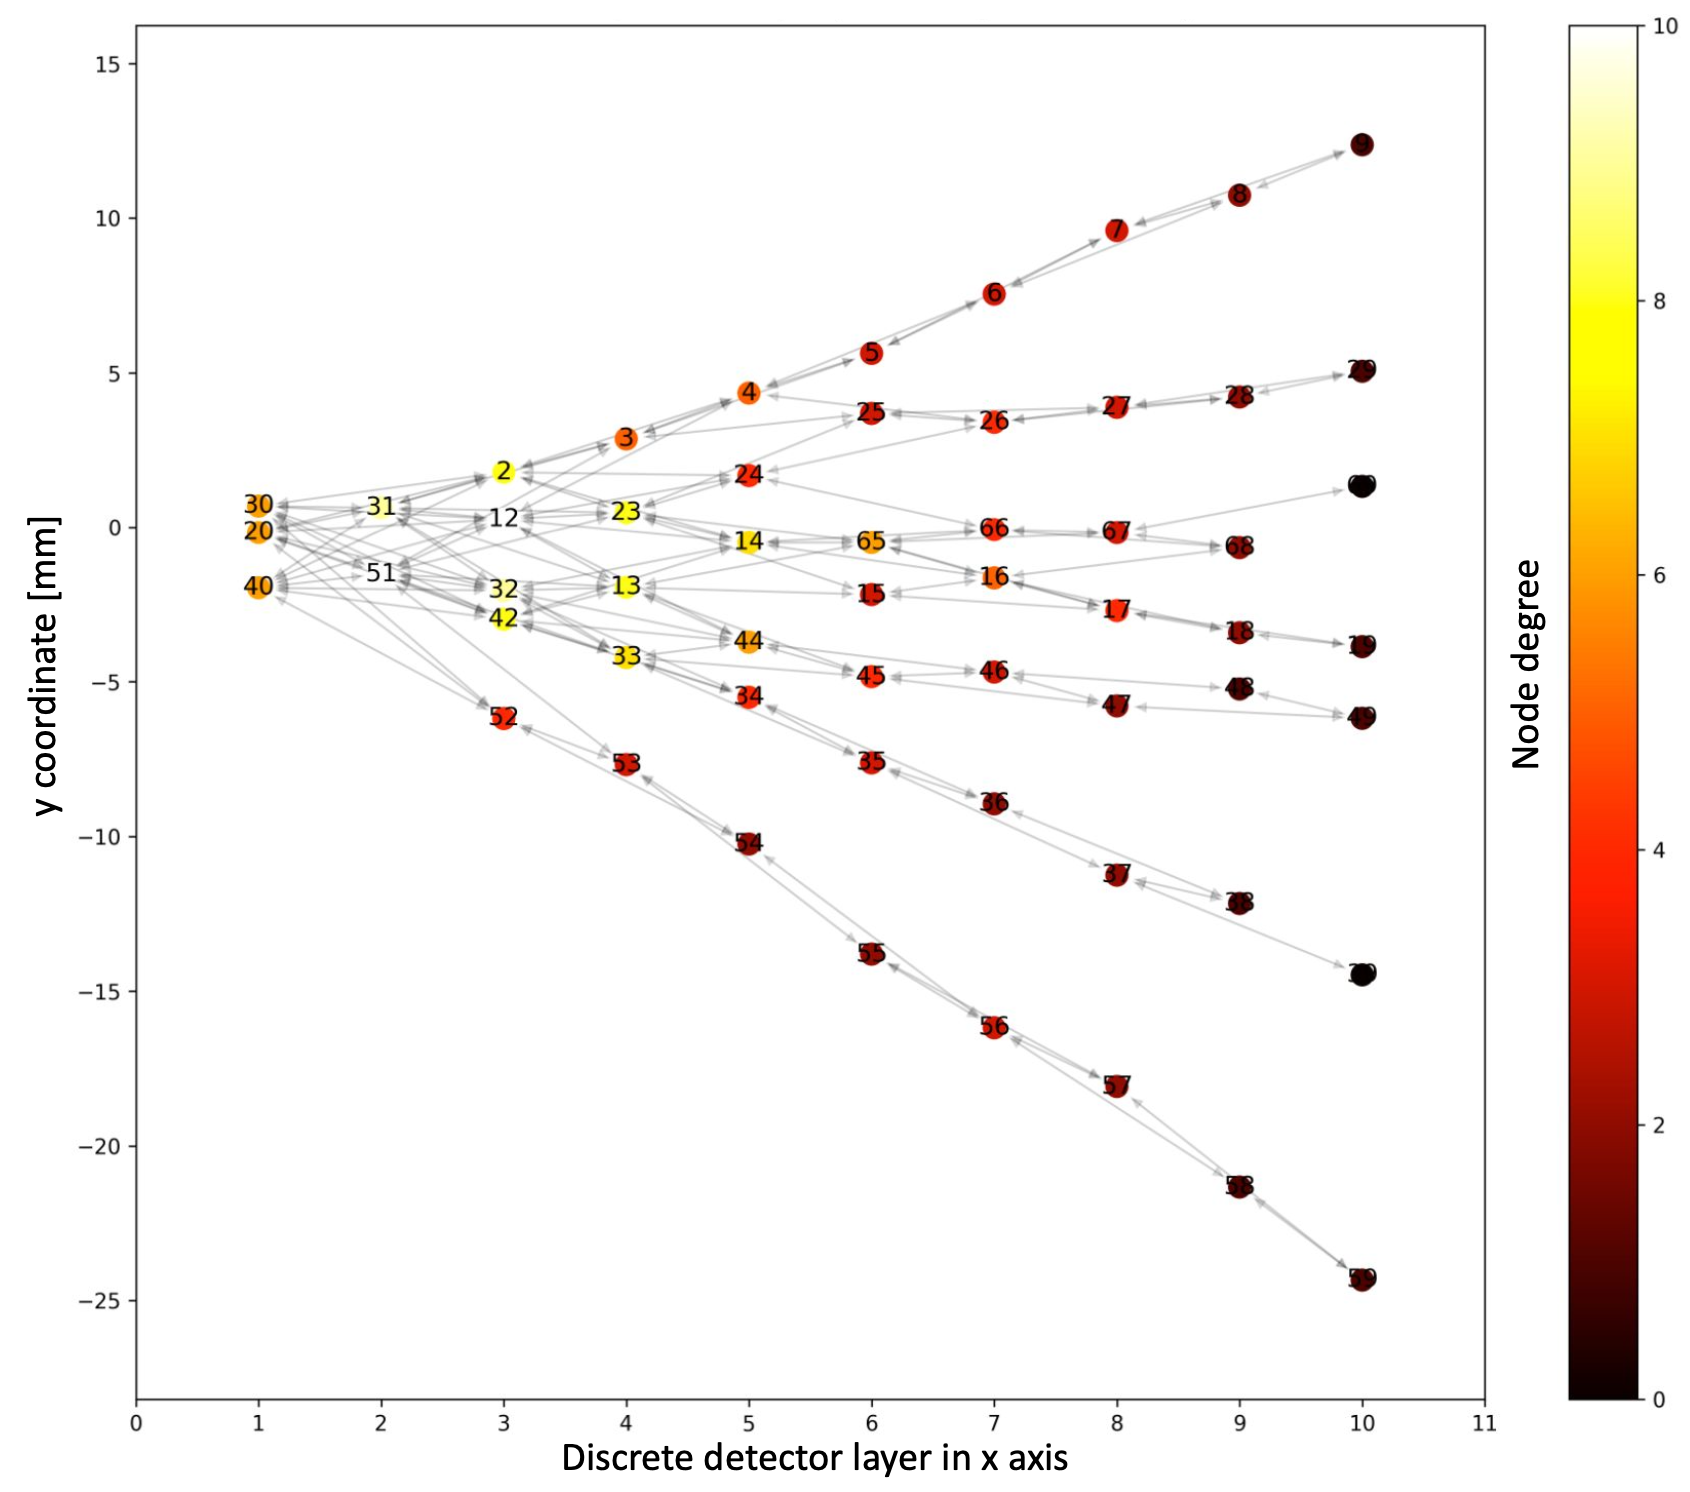
\includegraphics[width=0.99\textwidth]{images/5-gnn-algorithm/heatmap-network.png}
    \caption{Conversion of simulated hits in Figure \ref{fig:ground-truth} to a graph network, plotted as a node-degree heat map using the model in Eq \eqref{eqn:mc-toy-measurement-model}. Edge connections are formed using a pair predictor. The heat map represents node degree, where ``hot'' nodes (white-yellow) contain many edge connections, whereas ``cold'' nodes (orange-red) contain fewer edge connections.}
    \label{fig:heat-map}%
\end{figure}


\subsubsection{Graph Network Initialization}

The network is initialised with track state estimates, $X_{ij}$, given by Eq \eqref{eqn:track-state-estimate} and MC truth information at each node. Each connection is modelled as a straight line, where $X_{ij}$ comprises the $y$-measurement at node $i$, given by $m_i$, and the track inclination to its neighbour node $j$, given by $\tau_{ij} = (m_i - m_j) / (x_i - x_j)$, so that

\begin{equation}
X_{ij} = \begin{bmatrix} m_i \\ \tau_{ij} \end{bmatrix}
\label{eqn:track-state-estimate}
\end{equation}


The joint measurement covariance matrix, $S$, is stated in Eq. \eqref{eqn:track-state-estimate-2}, where $\sigma_0$ = 100 $\mu$m. Negligible uncertainty is assumed in the $x$-measurement due to the low thickness of pixel sensors. The state covariance, $C_{ij}$, is derived using the standard linear algebra approach, where $C_{ij} = GSG^T$, where matrix $G$ is the Jacobian which relates the measurements to the state vector, $X_{ij}$, using a linear extrapolation, where $dx = x_i - x_j$.  

\begin{equation}
S = \begin{bmatrix} \sigma_0^{2} & 0 \\ 0 & \sigma_0^{2} \end{bmatrix}  \quad G = \begin{bmatrix} 1 & 0 \\ dx^{-1} & -dx^{-1}  \end{bmatrix}
\label{eqn:track-state-estimate-2}
\end{equation}


\subsubsection{Implementation of Track State Extrapolation}

During Stage 1: GMR, $X^{M}$ and $C^{M}$ are computed using Eq \eqref{eqn:inverse-variance-weighting}. During Stage 2: Information Aggregation, $X^M$ is projected into the subspace of measurements using the measurement vector $H = [1 \quad 0]$. The residual, $r_{ij}$, between the projection, $HX^M$, and the measurement at each node is calculated using Eq \eqref{eqn:residual}

\begin{equation}
r_{ij} = m_i - HX_{ij}^M
\label{eqn:residual}
\end{equation}

The covariance of the residual, $V_{ij}$, is given by Eq. \eqref{eqn:covariance-of-residual}

\begin{equation}
{V}_{ij} = H \widetilde{C}_{ij} H^{T} + \sigma_{0}^{2}
\label{eqn:covariance-of-residual}
\end{equation}

where the extrapolated covariance, $\widetilde{C}_{ij}$, is calculated using Eq \eqref{eqn:extrapolation} with process noise, $Q$, defined as the zero matrix. The corresponding Mahalanobis distance is given by Eq \eqref{eqn:mahalanobis-distance}, and the distribution can be seen in Figure \ref{fig:mahalanobis-threshold-toy-model}.

\begin{equation}
\Delta \chi_{ij}^{2} = r_{ij}^{T} {V}_{ij}^{-1} r_{ij}
\label{eqn:mahalanobis-distance}
\end{equation}


% \begin{figure}[htbp]
\begin{figure}[H]
    \centering
    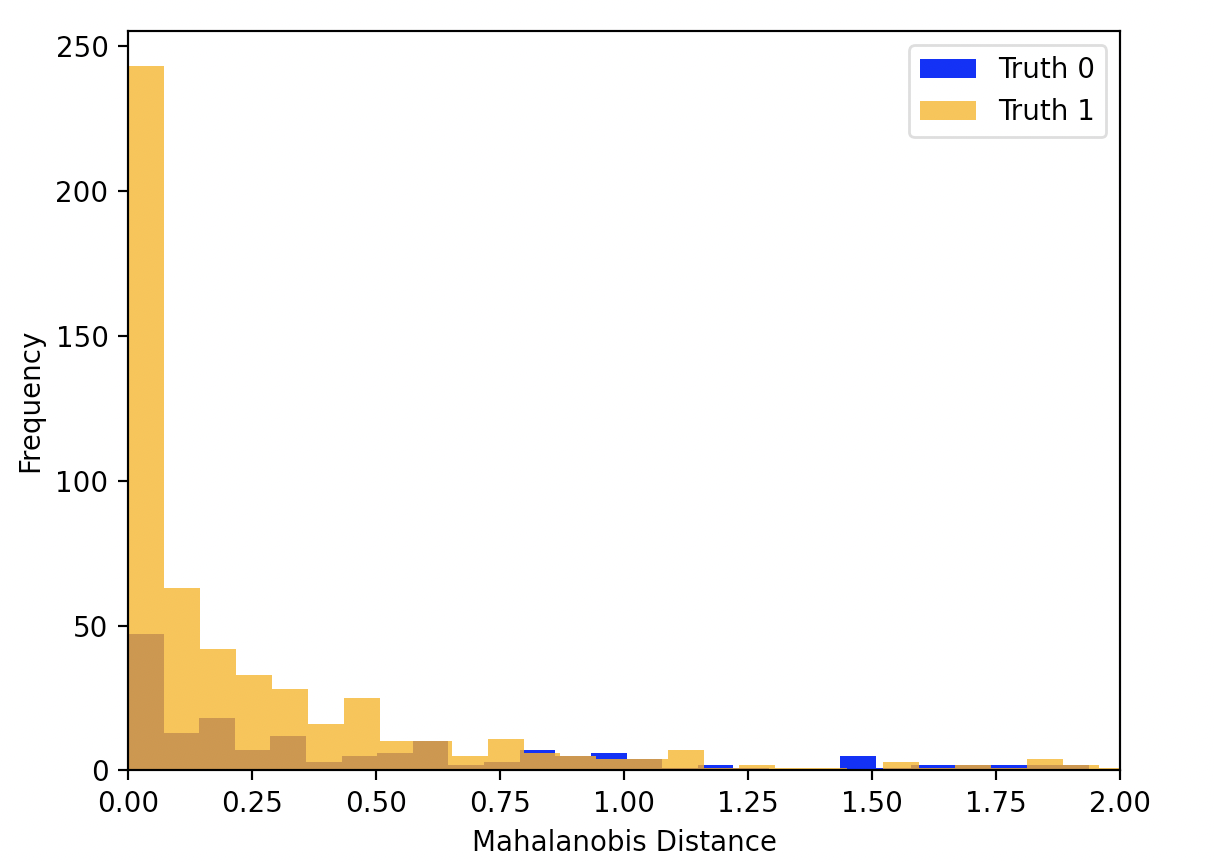
\includegraphics[width=0.96\textwidth]{images/5-gnn-algorithm/mahalanobis-threshold-toy-model-2.png}
    \caption{Mahalanobis distance, $\Delta \chi^{2}$, computed between the projected state and the measurement at each node, during state extrapolation for the GNN algorithm applied to a simple toy MC model. Truth 1 shows the distribution where the truth particle originating from the extrapolated state and the truth particle originating from the measurement are the same, and truth 0 otherwise.}
    \label{fig:mahalanobis-threshold-toy-model}%
\end{figure}



Using Figure \ref{fig:mahalanobis-threshold-toy-model}, a distance of 1.0 is selected as a threshold for accepting extrapolated states, as this provides 95\% efficiency on selecting the truth 1 class. If $\Delta \chi_{ij}^{2} < 1.0$, then $X^M$ is extrapolated to its neighbour node using the KF update. The extrapolated state, $\widetilde{X}_{ij}$, is calculated by the KF using Eq \eqref{eqn:extrapolation}, defined as the linear extrapolation from node $j$ to node $i$. This is described by $m_i = m_j + \tau_j dx$ and $\tau_i = \tau_j$. Therefore, the derived Jacobian, $\hat{F}$, for the KF is given by Eq \eqref{eqn:mc-model-F}.

% Jacobian F is derived by differentation of m_i and t_i equations with respect to initial parameters m_j and t_j

\begin{equation}
\hat{F} = \begin{bmatrix} 1 & dx \\ 0 & 1 \end{bmatrix}
\label{eqn:mc-model-F}
\end{equation}



\subsubsection{Implementation of KF for Track Extraction}

For a set of $n$ nodes representing a track candidate, the sequential set of measurements are $\{m_{(n-1)}, ..., m_1, m_0 \}$, where $m_{(n-1)}$ is the measurement of the node with the largest radius. The KF for track extraction is initialised with the following two-dimensional filter state estimate, $\hat{x}$, given by Eq \eqref{eqn:kf-toy-model-x-init}.

\begin{equation}
\hat{x} = \begin{bmatrix} m_{(n-1)} \\ \tau_{(n-1)} \end{bmatrix}
\label{eqn:kf-toy-model-x-init}
\end{equation}

where the track position measurement, $m_{(n-1)}$, is known and the track inclination, $\tau_{(n-1)}$, is initialized to zero as track inclination information is unknown at the start of the filter. The filter covariance matrix, $\hat{P}$, is initialised using Eq \eqref{eqn:mc-model-P-init-covariance}

\begin{equation}
\hat{P} = \begin{bmatrix} \sigma_0^{2} & 0 \\ 0 & \sigma_{\tau}^2 \end{bmatrix}
\label{eqn:mc-model-P-init-covariance}
\end{equation}

where $\sigma_{\tau}^2$ is the variance in the track inclination, $\tau$, and is initialized to $10^3$. The measurement error in the KF, $\hat{R}$, is attributed to the error due to the measurement of the $x$-$y$ plane and is initialised to $\sigma_{0}$ = 100 $\mu$m. The transition Jacobian in the KF uses the linear model and is given by Eq \eqref{eqn:mc-model-F}. The measurement vector is given by $\hat{H} = [1 \quad 0]$ and the process noise matrix is set to $\hat{Q} = 0$.



\subsubsection{Results}

Figure \ref{fig:example-application-1} shows an example of the GNN algorithm applied to the toy model in Figure \ref{fig:heat-map}. Figure \ref{fig:mc-example-1} displays the graph network where an initial CCA has been applied. Three smaller subgraphs have been identified as shown by separate colours. Nodes with $\sigma_e^2 > 0.8$ are not shown as clustering was not possible. The subsequent extracted track candidates are shown in Figure \ref{fig:mc-example-2}, where seven distinct tracks are observed. A precision of 60\% was achieved on identifying correct outlier connections with respect to the MC truth during stage 1. This simulation shows 100\% efficiency of track reconstruction with respect to MC truth, as all seven truth tracks were extracted in two stages. 

Figure \ref{fig:example-application-2} shows another simulation of the MC toy track model with application of the GNN algorithm. The application of CCA yields two distinct subgraphs shown in Figure \ref{fig:mc-example-3} by two separate colours. The subsequent extracted track candidates are shown in Figure \ref{fig:mc-example-4}, where six distinct tracks can be observed. A precision of 65\% was achieved on identifying correct outlier connections with respect to the MC truth during stage 1. A fast convergence was achieved in extracting six out of seven track candidates after the first stage of the algorithm. Remaining networks were propagated to further stages, however no further track candidates were extracted. Similarly, nodes with $\sigma_e^2 > 0.8$ are not shown here, as clustering was not possible. This suggests that $\sigma_{e}^{2}$ is an important discriminating feature when clustering track state estimates. 

Within this simple example, the GNN-based algorithm was not continued beyond stage 2. The main aim was to illustrate that the iterative methodology of the GNN framework is successful in identifying outlier edge connections as the graph network evolves, and allows track candidates to become easily identifiable. The purpose here was not to reconstruct the entire track candidate in all pixel layers of this model (nodes with $\sigma_e^2 > 0.8$). This task would require further analysis and optimisation of hyperparameters. At the time of writing, investigation of the application of the GNN-based algorithm on a realistic detector setup with much greater hit multiplicity was prioritised. Proper tuning of hyperparameters is done for the TrackML detector model, discussed further in Chapter \ref{chapter-6}. 


%\begin{center}
\begin{figure}[htbp]%
    \centering
    \subfloat[\centering Simulated graph network post CCA]{{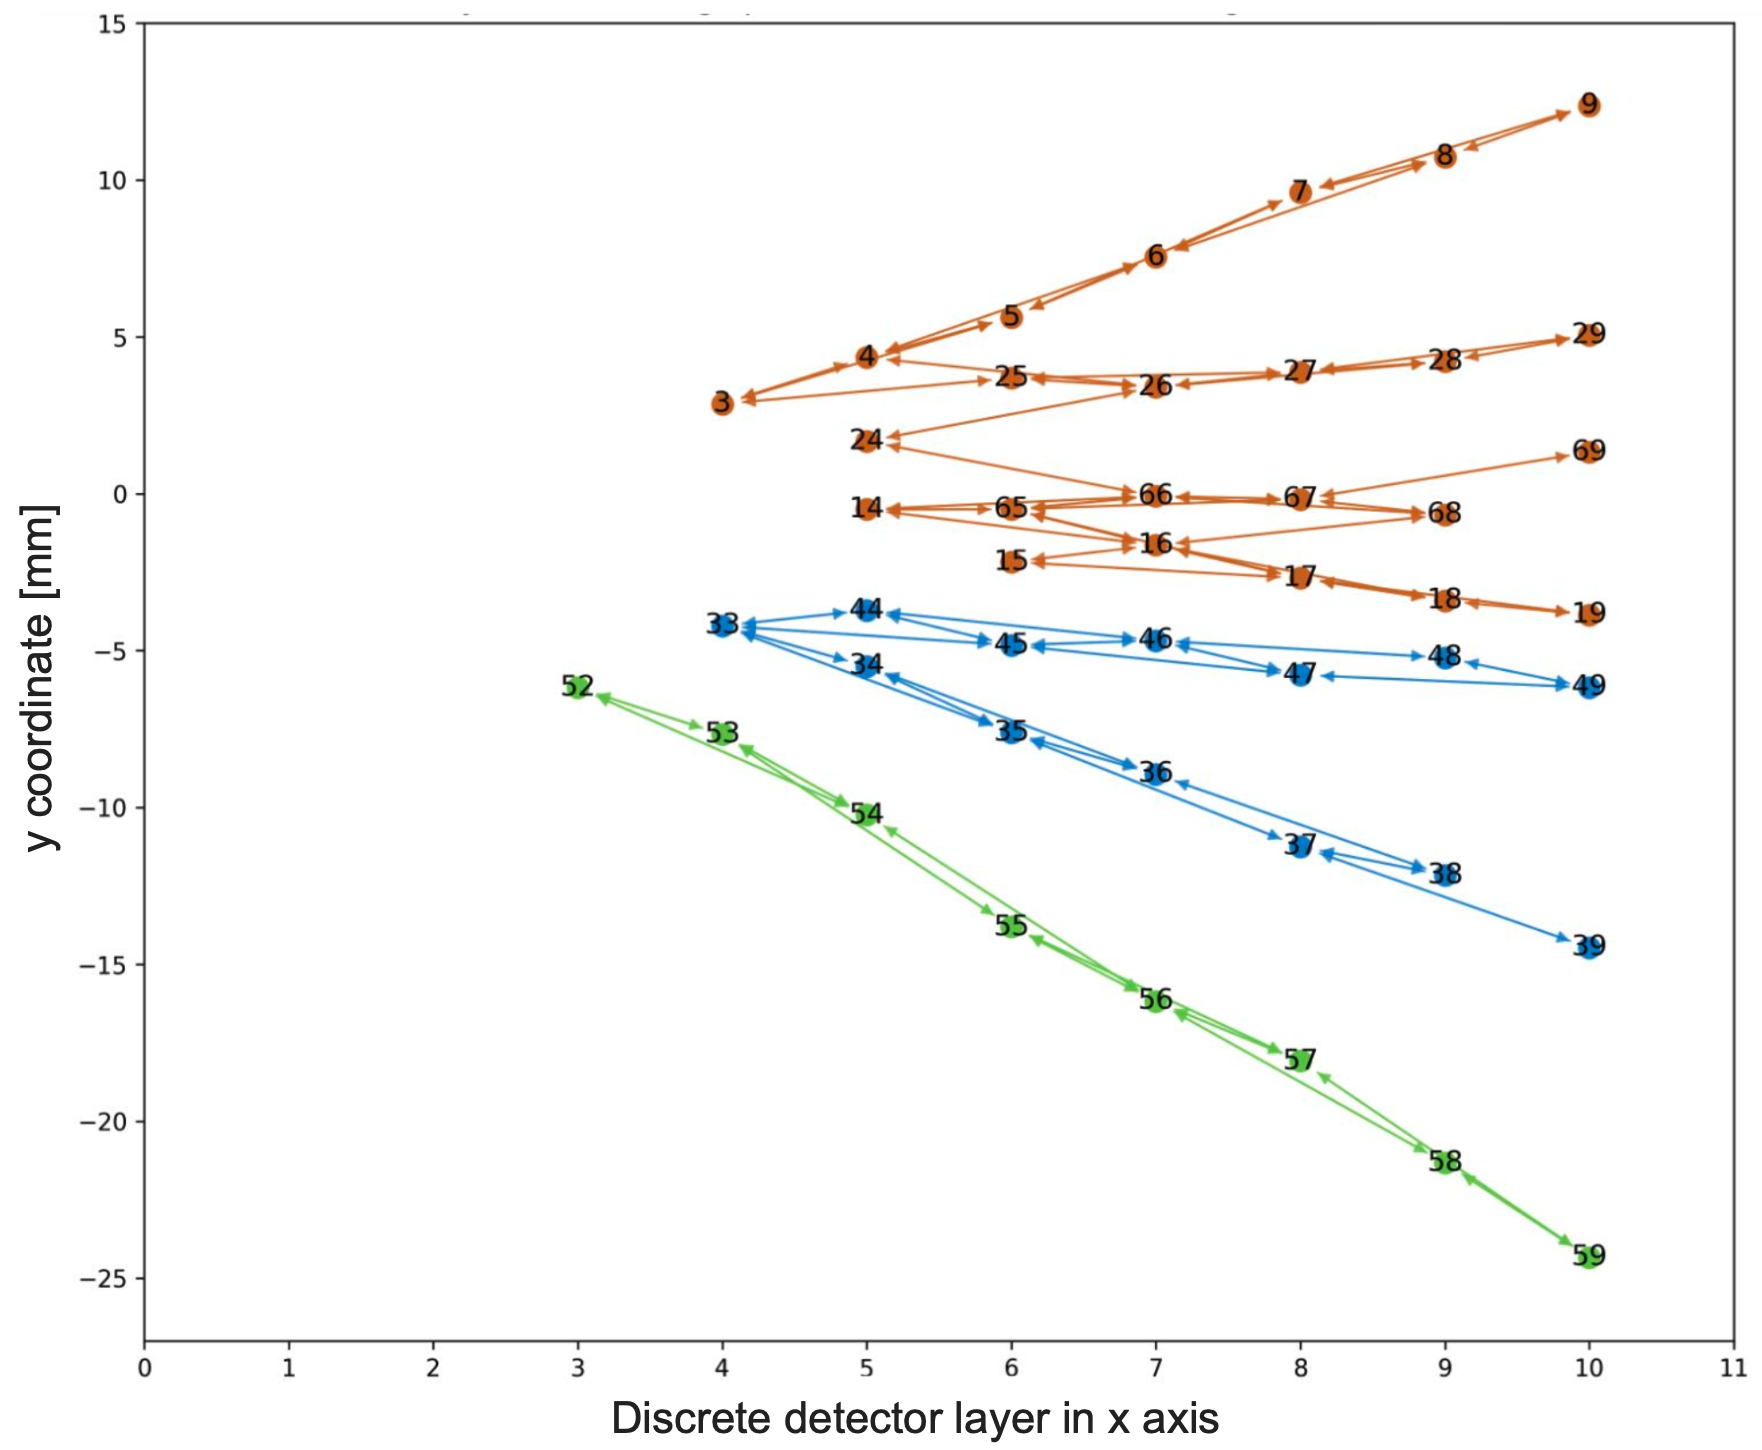
\includegraphics[width=11.8cm]{images/5-gnn-algorithm/mc-example-1a.png} } \label{fig:mc-example-1}}%
    \hfill
    %\qquad
    \subfloat[\centering Extracted track candidates at each stage of the GNN algorithm]{{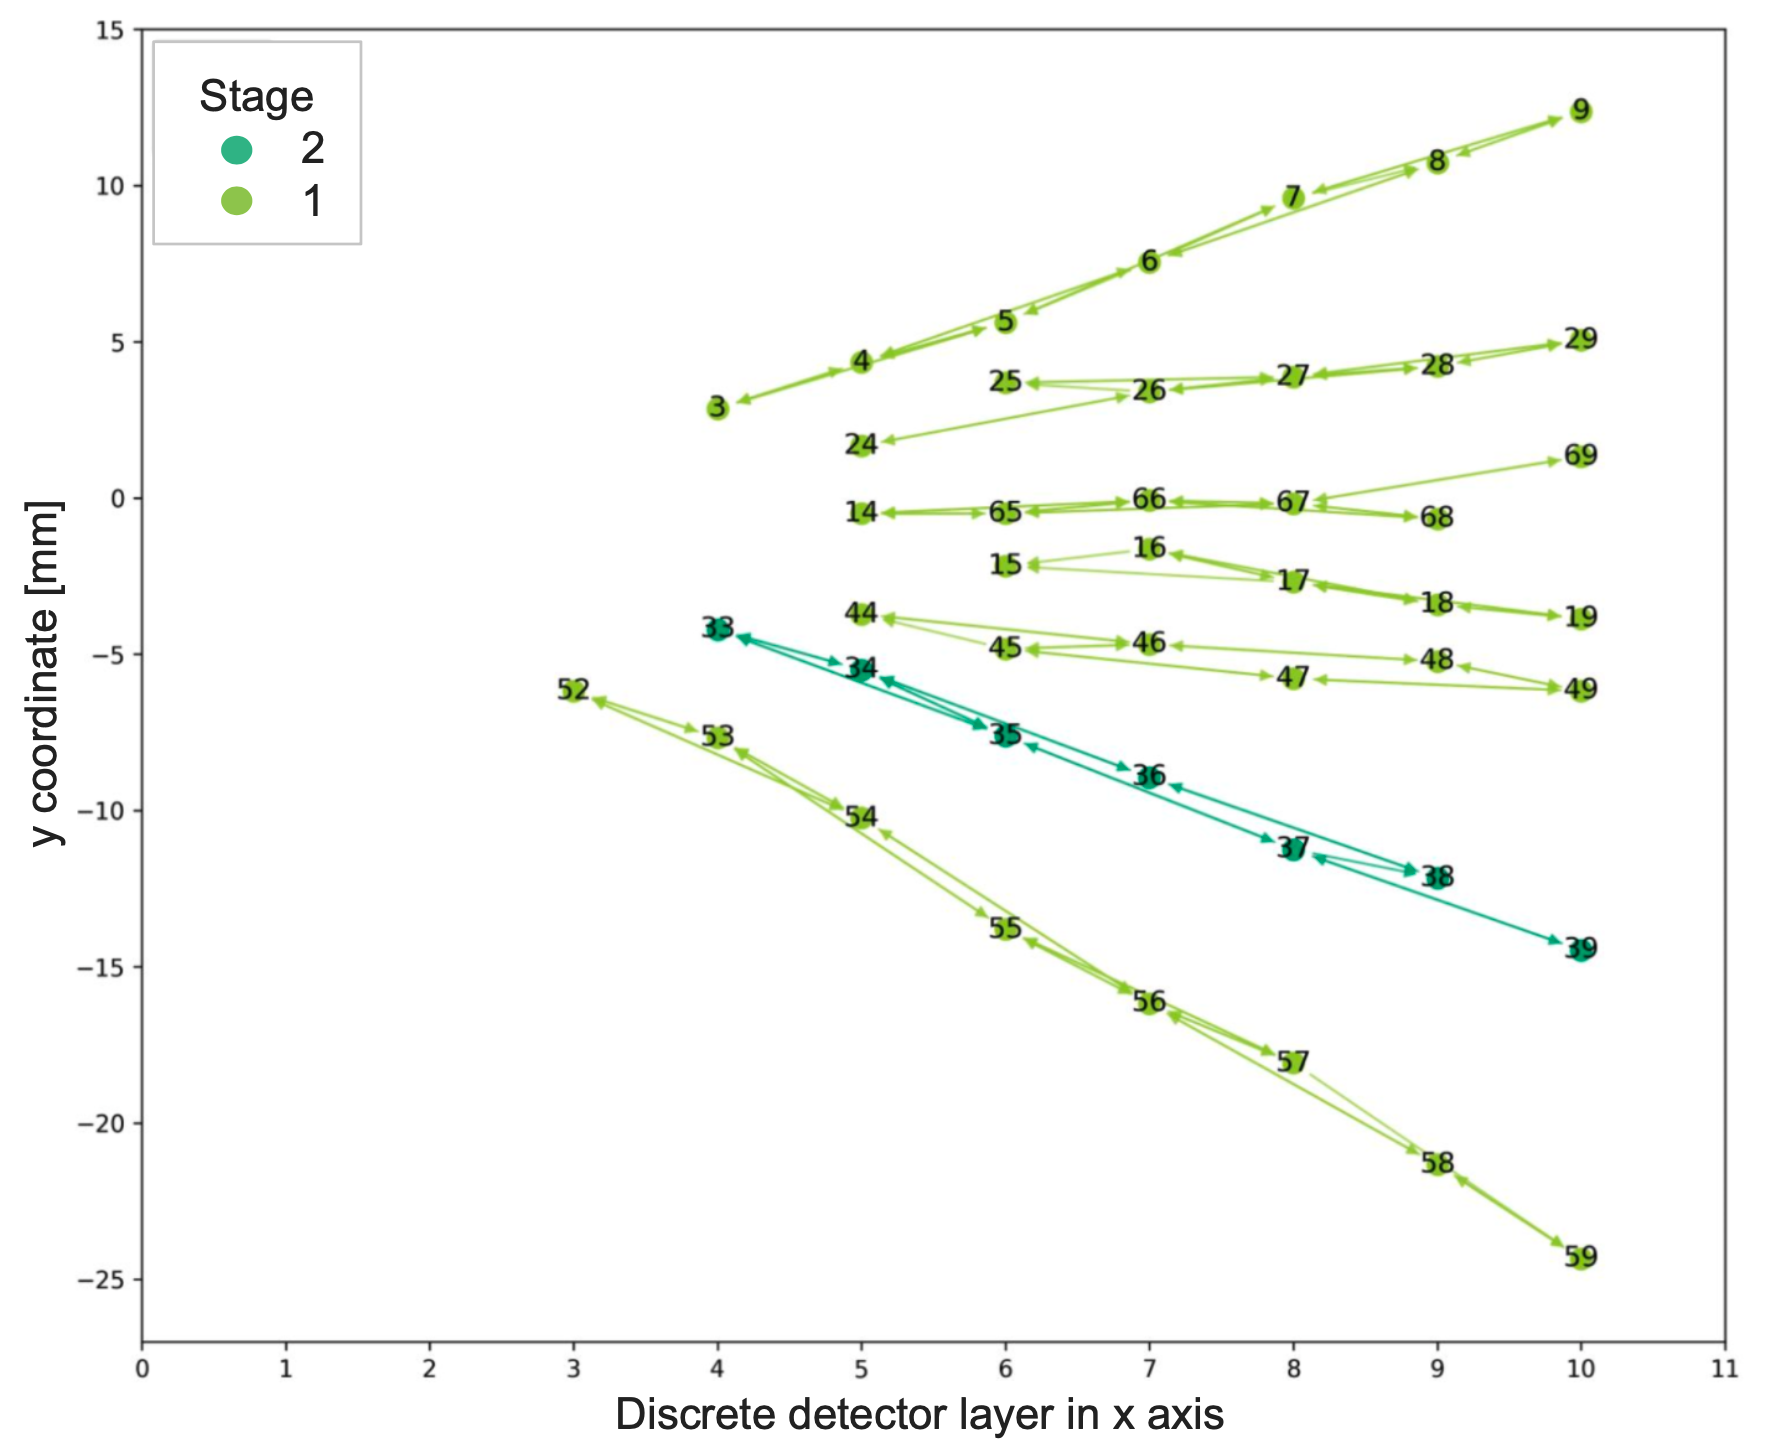
\includegraphics[width=12.1cm]{images/5-gnn-algorithm/mc-example-2a.png} } \label{fig:mc-example-2}}%
    \caption{Results of the GNN-based algorithm applied to a simple MC simulation. a) The simulated graph network where nodes with $\sigma_e^2 > 0.8$ are not plotted as clustering was not possible for these nodes. A CCA was applied to split the graph network into smaller subgraphs, where each colour indicates a different subgraph. b) The extracted track candidates after the applied GMR and Information Aggregation stages, where seven separate track candidates can be seen.}%
    \label{fig:example-application-1}%
\end{figure}
%\end{center}

%\begin{center}
\begin{figure}[htbp]%
    \centering
    \subfloat[\centering Simulated graph network post CCA]{{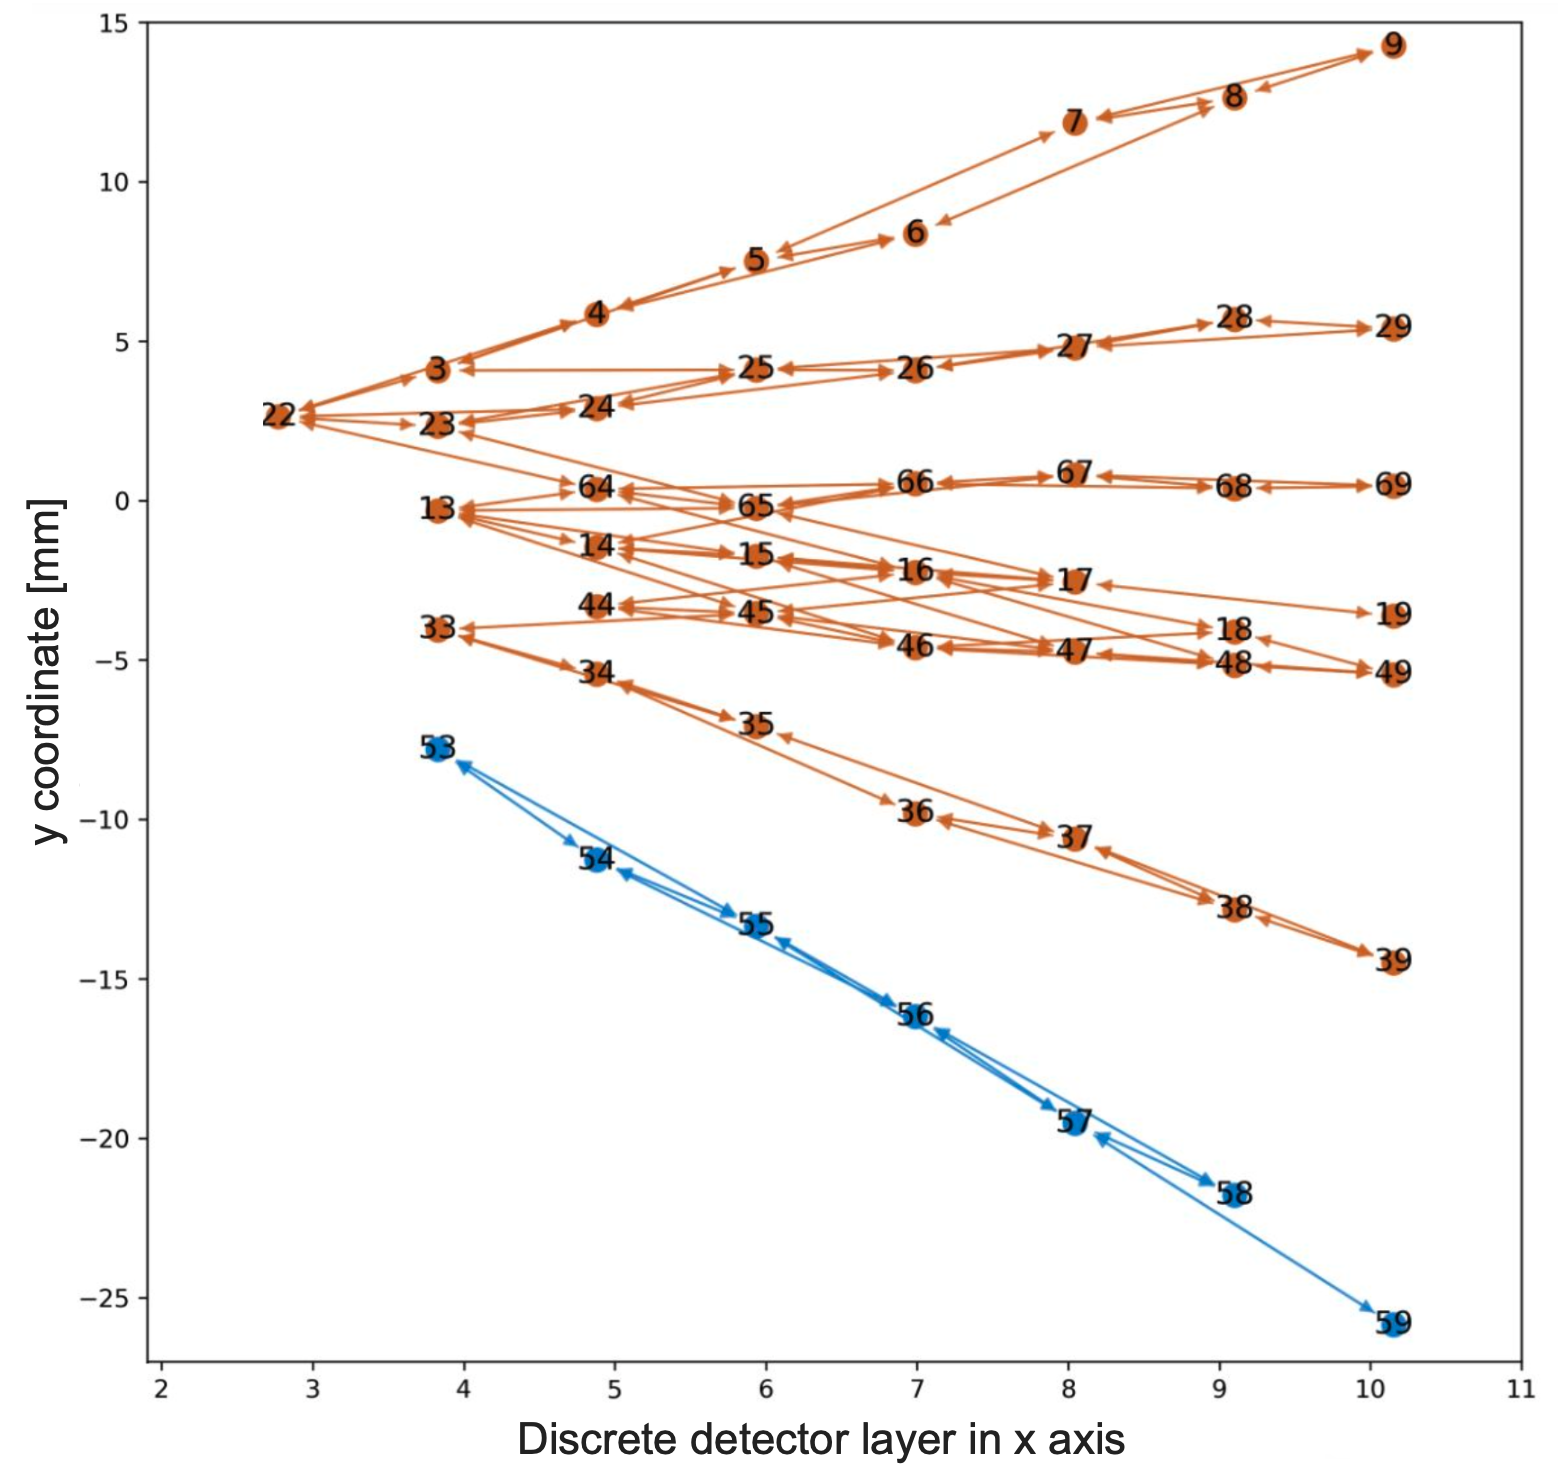
\includegraphics[width=10.7cm]{images/5-gnn-algorithm/mc-example-3a.png} } \label{fig:mc-example-3}}%
    \hfill
    %\qquad
    \subfloat[\centering Extracted track candidates after stage 1]{{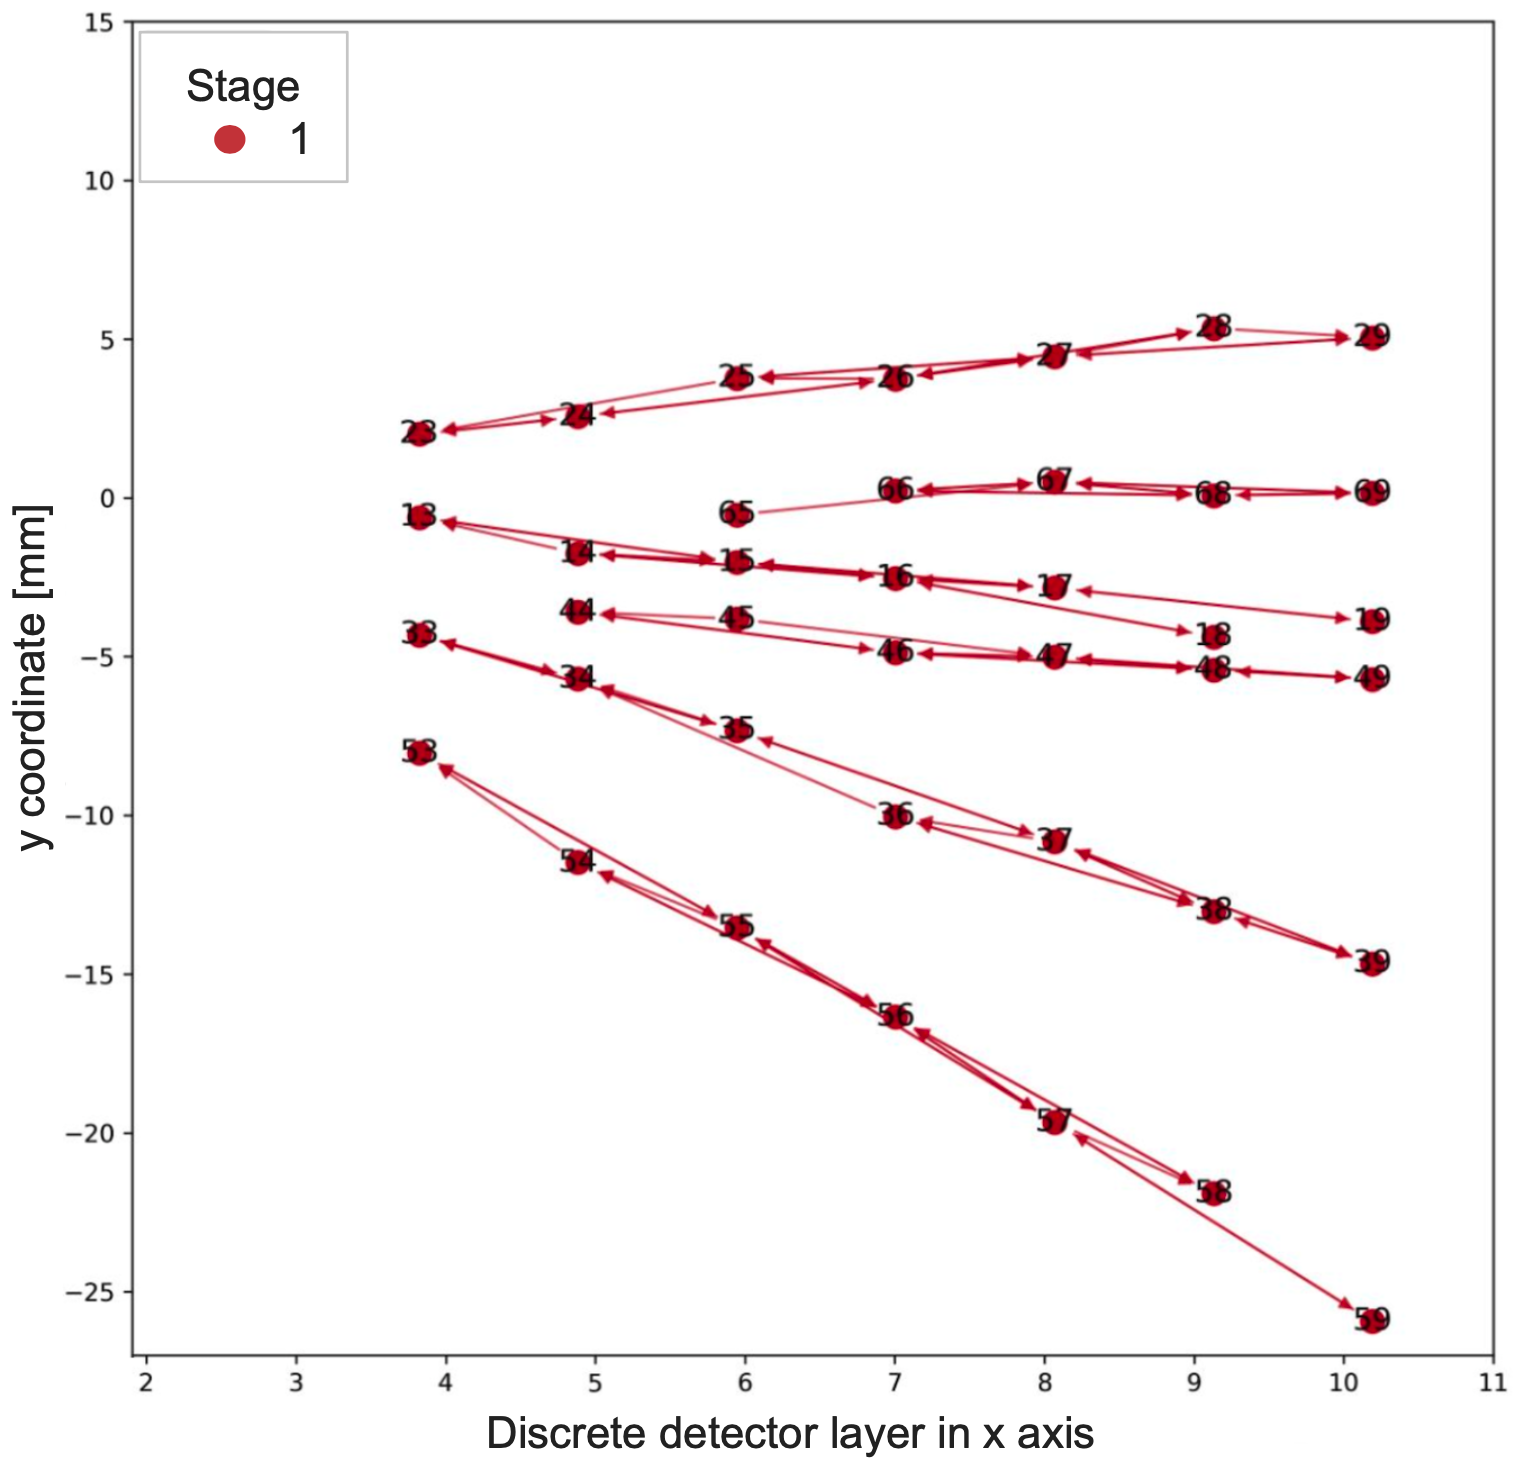
\includegraphics[width=10.8cm]{images/5-gnn-algorithm/mc-example-5a.png} } \label{fig:mc-example-4}}%
    \caption{Results of the GNN-based algorithm applied to a simple MC simulation a) The simulated graph network where nodes with $\sigma_e^2 > 0.8$ are not plotted as clustering was not possible. A CCA was applied to split the graph network into smaller subgraphs, where each colour indicates a different subgraph. b) Six extracted track candidates after the GMR stage.}%
    \label{fig:example-application-2}%
\end{figure}
%\end{center}

\newpage
\section{Conclusion}

The proposed GNN algorithm is successful in iteratively identifying outlier edge connections and extracting track candidates for simple simulated particle collision events. GMR via clustering of state vectors proves to be a successful first step towards resolving incompatible connections in the network. The KF works well for both the extrapolation of state vectors to neighbour nodes, as well as for track extraction and track fitting. This ensures neighbourhood information can be aggregated in order to improve the precision in track state parameters. An intrinsic characteristic of the GNN algorithm is that neighbourhood complexity is inferred by the network. This is observed as the GNN algorithm automatically initiates the pattern recognition process in regions where outlier connections are easily identifiable. The network starts with low density regions and gradually progresses towards high density areas. This indicates that the GNN algorithm behaves as expected, first resolving ambiguities in ``cold'' regions and shows great promise for extraction of track candidates in more complex cases and realistic detector setups.


%It was observed that clustering of states was not always possible in all ``hot'' regions. As a result, the pattern recognition process was automatically initiated in regions where outlier connections were easily identifiable, i.e. ``cold'' regions. This indicates that the GNN algorithm behaves as expected, as the network starts with low density regions and gradually progresses towards high density areas.

%---------------------------------------------
%	6. Application & Perform of GNN Algorithm
%---------------------------------------------

%WIt allowed us to generate realistic data emulating a full Silicon LHC detector (see Fig 3), while providing us with the ground truth of particle trajectory membership. Thus, for each event we obtained the... and, as ground truth, the list of points associated to each track. There is a one to one relationship between the true 3D points and the reconstructed ones.

\chapter{GNN Algorithm Implementation for the TrackML Model}
\label{chapter-6}

This chapter focuses on the implementation of the GNN pattern recognition algorithm to the publicly available dataset designed for the Kaggle TrackML challenge \cite{kaggle-trackml}. The TrackML detector emulates a full silicon LHC detector and as such, certain models of the GNN algorithm outlined in Chapter \ref{chapter-5}, are improved for the TrackML detector geometry. Section \ref{chapter-6-data-prep} describes the structure of the TrackML data and how it was used to build a graph network. Sections \ref{constructing-track-states} and \ref{chapter-6-covariance-derivation} describe the construction of track state estimates. Section \ref{chapter-6-kl-threshold} presents the classifier constructed to determine the optimal KL threshold used within the GMR stage. Finally, Section \ref{chapter-6-extrapolation-track-extraction} presents alterations to the extrapolation models used within the Information Aggregation stage, as well as the KFs used within track fitting. 
 


\section{Data Preparation}
\label{chapter-6-data-prep}

The TrackML dataset \cite{kaggle-trackml-data} comprises multiple independent events, where each event contains simulated measurements (3D points) of particles generated in a collision between proton bunches at the LHC. The training dataset contains the recorded hits and the measured position of each corresponding hit in the global Cartesian coordinate system $(x, y, z)$. The event truth data contains each hit's ground truth counterpart, their association to particles and the initial parameters of those particles. The radius at a given point on the particle's trajectory, $r$, is computed using the square root of the sum in quadrature of the global $x$ and $y$ measurements.

In order to read the TrackML data, Python scripts provided by the Kaggle competition organisers are used \cite{python-scripts-kaggle}. The TrackML data provide hit information only, such that graph nodes and edges must be created independently. The hits are converted into graph nodes and edge pairs are constructed using the \textit{FASTrack} algorithm used during the throughput phase of the TrackML Kaggle competition \cite{Amrouche2023}. The FASTrack algorithm is based on a similar hit-pair predictor methodology outlined in Chapter \ref{chapter-4}, whereby hit cluster shapes are used to predict the intervals of track inclination angles and save CPU time by avoiding hit combinations with parameters incompatible with the prediction. Graph edges are predicted and can span up to two layers apart.

Due to the sheer volume of data generated during high-energy proton-proton collisions, it is impossible for any Trigger system to reconstruct all objects. There are many low momentum tracks that will produce hits and will begin to curve under the influence of the magnetic field. These types of tracks are not of interest for reconstruction within this study. As a result, there are certain kinematic requirements imposed. Constraints are embedded on the graph edge parameters, in order to select the tracks of interest with a particular $p_{\text{T}}$ from the very beginning \cite{Dmitry-fasttrack-addtest}, and construct the graph network. 

% min_Curvature - want to select a particular pT range of the tracks we want to look at
% repo - "fasttrack" add-test branch


\section{Construction of Track State Estimates}
\label{constructing-track-states}

Track state estimates, $X_{ij}$, are constructed using a parabolic model for parameters in the transverse $x$-$y$ plane and a linear model for parameters in the $r$-$z$ plane.

% In order to construct track state estimates, $X_{ij}$, for each connection between node $i$ and its neighbour $j$, track parameters in both the transverse $x$-$y$ plane and the $r$-$z$ plane are considered.


\subsection{Parabolic Track Model}
\label{parabolic-state}

In the $x$-$y$ plane, charged particles experience the influence of the magnetic field and their trajectories follow a near-circular shape, which can be approximated by a parabola for relatively high $p_{\text{T}}$ ($> 1$ GeV) tracks. As illustrated in Figure \ref{fig:gnn-parabolic-model}, a parabola is formed under the assumption that the particle trajectory goes through the global origin O, node A and neighbour node B. The parabola is transformed into the local coordinate system of node A such that the new $x$-axis, $X_A$, is parallel to O - A and the new $y$-axis, $Y_A$, is the perpendicular. 

\begin{figure}[htbp!] 
    \centering
    \subfloat[]{%
        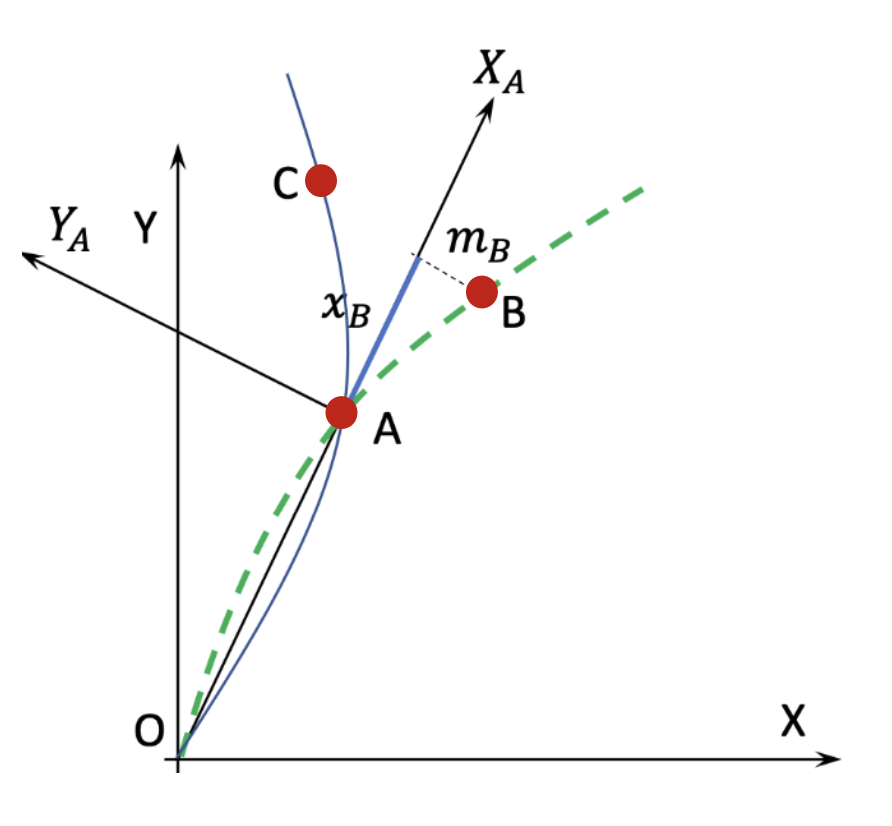
\includegraphics[width=0.42\textwidth]{images/6-trackml/parabolic-state-model-1.png}%
        \label{fig:gnn-parabolic-state-1}%
        }%
    \hfill%
    \subfloat[]{%
        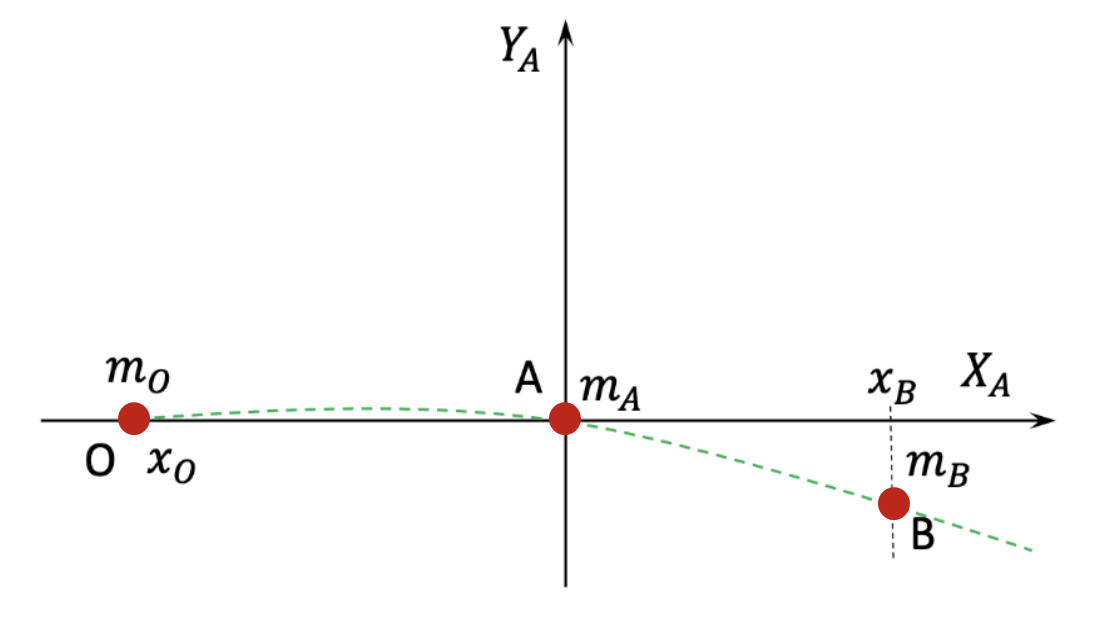
\includegraphics[width=0.56\textwidth]{images/6-trackml/parabolic-state-model-2.png}%
        \label{fig:gnn-parabolic-state-2}%
        }%
    \caption{Parabolic model illustration. a) Construction of example parabolas O - A - B and O - A - C, where O is the global origin and A, B, C are graph nodes. b) Rotation of parabola O - A - B into the local coordinate system of A.}
    \label{fig:gnn-parabolic-model}
\end{figure}


Using the quadratic equation of a parabola, the vector of measurements in the local coordinate system of node A, $ m = [m_O \quad m_A \quad m_B]^{T}$ can be expressed in terms of the unknown parabolic coefficients $p = [a \quad b \quad c]^{T}$ using Eq \eqref{eqn:parabolic-equations}, 

\begin{equation}
    m = H p 
    \label{eqn:parabolic-equations}
\end{equation}

where $m_O$, $m_A$ and $m_B$ are the respective measurements of the global origin O, node A and node B, transformed into the local coordinate system of node A, and $\{a, b, c\}$ are the parabolic coefficients. In this new frame of reference, measurements $m_O = 0$ and $m_A = 0$ as illustrated in Figure \ref{fig:gnn-parabolic-state-2}. The measurement matrix, $H$, relates the measurement vector, $m$, to the vector of parabolic parameters, $p$, and is given by Eq \eqref{eqn:trackml-matrix-h-xy},

\begin{equation}
    H = \begin{bmatrix} x_O^{2} & x_O & 1 \\ 0 & 0 & 1 \\ x_B^{2} & x_B & 1 \end{bmatrix} 
    \label{eqn:trackml-matrix-h-xy}
\end{equation}

where $x_O$ and $x_B$ are the $x$-coordinates of global origin O and node B in the local coordinate system of node A. The parabolic parameters are derived using Eq \eqref{eqn:derive-p}.

\begin{equation}
    p = H^{-1} m 
    \label{eqn:derive-p}
\end{equation}


% \begin{equation}
% \begin{aligned}
% m_O = ax_{O}^{2} + bx_O + c \\
% m_A = c \\
% m_B = ax_{B}^{2} + bx_B + c
% \end{aligned}
% \label{eqn:parabolic-equations}
% \end{equation}


\subsection{Linear Track Model}
\label{linear-state}

The $r$-$z$ plane is parallel to the direction of the beamline where tracks follow a linear model, as the influence of the solenoidal magnetic field is negligible. The inverse track inclination, $\tau$, between node A and neighbour B, is given by Eq \eqref{eqn:tau-parameter}, where $(z_A, r_A)$ refer to measurements of node A and $(z_B, r_B)$ refer to measurements of neighbour node B.

\begin{equation}
\tau = \frac{z_A - z_B}{r_A - r_B}
\label{eqn:tau-parameter}
\end{equation}

\subsection{Combined Track State Estimate}

Parabolic parameters $\{a, b\}$ derived in Section \ref{parabolic-state}, as well as the inverse track inclination, $\tau$, given in Eq \eqref{eqn:tau-parameter}, provide an indication of track orientation. Hence, the track state estimate, $X_{ij}$, at node $i$ given neighbour $j$ is defined by Eq \eqref{eqn:joint-state-vector}.

\begin{equation}
X_{ij} = \begin{bmatrix} a \\ b \\ \tau \end{bmatrix}
\label{eqn:joint-state-vector}
\end{equation}







\section{Derivation of Edge State Covariance}
\label{chapter-6-covariance-derivation}

To derive the edge state covariance, $C_{ij}$, of $X_{ij}$ given by Eq \eqref{eqn:joint-state-vector}, the covariance of the track state parameters in the $x$-$y$ and $r$-$z$ planes are handled separately. 


\subsection{Covariance of Parabolic Parameters}

The joint measurement covariance matrix, $S_{xy}$, for a parabola constructed in the $x$-$y$ plane using the global origin O and nodes A and B, as illustrated in Figure \ref{fig:gnn-parabolic-state-2}, is stated in Eq. \eqref{eqn:trackml-s-matrix-xy}


\begin{equation}
    S_{xy} = \begin{bmatrix} \sigma_O^{2} & 0 & 0 \\ 0 & \sigma_A^{2} & 0 \\ 0 & 0 & \sigma_B^{2} \end{bmatrix} 
    \label{eqn:trackml-s-matrix-xy}
\end{equation}

where $\sigma_O$, $\sigma_A$ and $\sigma_B$ are the respective errors due to the measurements at the global origin O, node A and node B, using the parabolic model approximation outlined in Section \ref{parabolic-state}. The measurement uncertainty in the global origin $\sigma_O$ is initialised to 4.0 mm due to the large uncertainty in the beamspot, whereas $\sigma_A$ and $\sigma_B$ are initialised to 0.3 mm due to the high precision of the pixel detector. The covariance of the vector of parabolic parameters, $p$, is given by $C_{xy}$ in Eq \eqref{eqn:c-xy} using the standard linear algebra approach.

\begin{equation}
    C_{xy} = H^{-1}S_{xy}{H^{-1}}^{T}
    \label{eqn:c-xy}
\end{equation}






\subsection{Variance in Inverse Track Inclination}
\label{variance-in-inverse-track-inclination}

The joint measurement covariance matrix, $S_{rz}$, for node $i$ and neighbour node $j$ in the $r$-$z$ plane is stated in Eq \eqref{eqn:trackml-s-matrix-rz}, where $\{ \sigma_{zi}, \sigma_{zj} \}$ are the measurement errors along the $z$-axis and $\{ \sigma_{ri}, \sigma_{rj} \}$ are the measurement errors in $r$, for the respective nodes $i$ and $j$. 

\begin{equation}
    S_{rz} = \begin{bmatrix} \sigma_{zi}^{2} & 0 & 0 & 0 \\ 
                             0 & \sigma_{zj}^{2} & 0 & 0 \\ 
                             0 & 0 & \sigma_{ri}^{2} & 0 \\
                             0 & 0 & 0 & \sigma_{rj}^{2}
                            \end{bmatrix} 
    \label{eqn:trackml-s-matrix-rz}
\end{equation}


The magnitude of the uncertainty in the $r$-$z$ plane is dependent on the detector layer where the graph node is situated. This is a result of the angle of incidence of the particle onto the detector layer, hence the layer's orientation will determine the magnitude of the error. For example, consider a barrel-located node; the uncertainty in the $z$-axis will be greater than the uncertainty in the $r$-axis due to the horizontal orientation of the barrel layer (vice versa for the endcap layer). Therefore, for a node located in the pixel barrel the following errors are used $\sigma_r = 0.4$ mm and $\sigma_z = 0.6$ mm. Conversely, for a node located in the pixel endcap the following errors are used $\sigma_r = 0.6$ mm and $\sigma_z = 0.4$ mm.

The uncertainty in the track inclination $\tau$ is computed using the standard error propagation and linear algebra approach. The transition Jacobian, $G$, relates the measurements in the $r$-$z$ plane to the inverse track inclination $\tau$ and is given by Eq \eqref{trackml-g-rz}.

% this applies to either node i or node j
% sigma0r = 0.4 --> error in r for barrel located node
% sigma0r = 0.6 --> error in r for endcap located node

% sigma0z = 0.6 --> error in z for barrel located node
% sigma0z = 0.4 --> error in z for endcap located node


\begin{equation}
    G = \begin{bmatrix} 
            (r_i - r_j)^{-1} \\
            -(r_i - r_j)^{-1} \\ 
            \frac{-(z_i - z_j)}{(r_i - r_j)^2} \\ 
            \frac{z_i - z_j}{(r_i - r_j)^2}
            \end{bmatrix} 
    \label{trackml-g-rz}
\end{equation}

The corresponding error in track inclination $\tau$ is given by Eq \eqref{eqn:error-in-tau}

\begin{equation}
    \sigma_{\tau} = G S_{rz} G^{T}
    \label{eqn:error-in-tau}
\end{equation}






\subsection{Moli\`ere Theory of Multiple Scattering}

A charged particle traversing a medium is deflected by many small-angle scatters. Most of this deflection is due to Coulomb scattering from nuclei. However, for hadronic projectiles the strong interactions also contribute to multiple scattering. Therefore, the uncertainty in track direction will have a contribution from multiple scattering, $\sigma_{ms}$. According to the theory of Moli\`ere, the scattering distribution is roughly Gaussian for small deflection angles. The contribution due to Moli\`ere multiple scattering is given by the simplified Highland formula \cite{moliere-theory-formula, Lynch:1990sq} stated in Eq \eqref{eqn:simplified-moliere-equation}.

%The Moli\`ere multiple scattering is inversely proportional to particle full momentum and proportional to the square root of material thickness.

% \begin{equation}
%     \sigma_{ms}^{2} = \frac{13.6 \text{MeV}}{\beta c p} z \sqrt{\frac{x}{X_0}} \left[ 1 + 0.038ln \left( \frac{x}{X_0} \right) \right] 
%     \label{eqn:moliere-equation}
% \end{equation}

\begin{equation}
    \sigma_{ms}^{2} = \frac{13.6 \text{MeV}}{\beta c p} z \sqrt{\frac{x}{X_0}}
    \label{eqn:simplified-moliere-equation}
\end{equation}

where $p$, $\beta c$, and $z$ are the full momentum, velocity, and charge number of the incident particle, and $x/X_0$ is the thickness of the scattering medium, measured in radiation lengths. For a relativistic particle, $\beta c \approx 1$ and the charge, $z$, is assumed to be 1. 




\subsubsection{Derivation of Full Momentum}

The full particle momentum, $p$, is given by Eq \eqref{eqn:full-momentum}

\begin{equation}
    p = p_\text{T} / \sin(\theta)
    \label{eqn:full-momentum}
\end{equation}

where $p_\text{T}$ is the transverse momentum of the particle and $\theta$ is the angle of inclination of the particle trajectory to the $z$-axis. The transverse momentum, $p_\text{T}$, for a charged particle in the presence of a magnetic field is given by Eq \eqref{eqn:transverse-momentum}

\begin{equation}
    p_\text{T} [\text{MeV/c}] = 0.3 B [\text{T}] \times q [\text{e}] \times r [\text{mm}]
    \label{eqn:transverse-momentum}
\end{equation}

The magnetic field strength of the TrackML model is given by $B$, the charge of the particle is given by $q$ and is set to 1, as shown in \cite{ATLAS-CONF-2010-072}. The radius, $r$, is inversely proportional to the track curvature $\kappa$, given by Eq \eqref{eqn:kappa}, 

\begin{equation}
\kappa = \frac{2a}{(1 + (2ax + b)^2)^{\frac{3}{2}}}
\label{eqn:kappa}
\end{equation}

where $\kappa$ is a function of parabolic parameters $a$ and $b$, and $x$ is the $x$-coordinate of the point at which the curvature is calculated. Therefore, the full momentum $p$ is given by Eq \eqref{eqn:full-momentum-derived} using the knowledge that $\kappa = 1/r$.

\begin{equation}
p = 0.3 B / \kappa \sin(\theta)
\label{eqn:full-momentum-derived}
\end{equation}

For the TrackML detector, the magnetic field strength, $B$, is 2 T.

\subsubsection{Orientation of Detector Layers}

If a particle crosses one of the TrackML detector layers at incident angle $\theta$, then the radiation length, $x/X_0$, is given by Eq \eqref{eqn:radiation-length}

\begin{equation}
x/X_0 = 0.02 f(\theta)
\label{eqn:radiation-length}
\end{equation}

where 0.02 is the integrated $x/X_0$ for a typical silicon detector layer, which is considered as a single thin scatter. The function $f(\theta)$ is determined by the orientation of the detector layer, on which the node-pair is located. For example, for a scattered node in the pixel barrel layer $f(\theta) = [\sin(\theta)]^{-1}$, and for a scattered node in the pixel endcap layer $f(\theta) = [\cos(\theta)]^{-1}$.




\subsubsection{Variance of Multiple Scattering}

The final form of the observed contribution of error due to multiple scattering is $\sigma_{ms}$, where the variance, $\sigma_{ms}^2$, is given by Eq \eqref{eqn:computed-multiple-scattering}.

\begin{equation}
    \sigma_{ms}^{2} = \frac{13.6 \text{MeV}}{0.3 B} \cdot \kappa \sin(\theta) \cdot \sqrt{0.02 f(\theta)}
    \label{eqn:computed-multiple-scattering}
\end{equation}



\subsection{Combined Edge State Covariance}

The edge state covariance matrix of the combined track state estimate $X_{ij}$, is given by $C_{ij}$ in Eq \eqref{eqn:combined-edge-state-covariance}.

\begin{equation}
    C_{ij} = \begin{bmatrix} 
            C_{xy}^{00} & C_{xy}^{01} & 0 \\ 
            C_{xy}^{10} & C_{xy}^{11} + \sigma_{ms}^2 & 0 \\ 
            0 & 0 & \sigma_{\tau}^{2} + \sigma_{ms}^2 \\
            \end{bmatrix} 
    \label{eqn:combined-edge-state-covariance}
\end{equation}

where $C_{xy}^{00}$, $C_{xy}^{01}$, $C_{xy}^{10}$ and $C_{xy}^{11}$ are the corresponding matrix components of the covariance of the vector of parabolic parameters $p$, $C_{xy}$, in the $x$-$y$ plane, stated in Eq \eqref{eqn:c-xy}, and $\sigma_{\tau}^2$ is the variance of the inverse track inclination $\tau$, stated in Eq \eqref{eqn:error-in-tau}. The combined edge state covariance, $C_{ij}$, is therefore represented as a 2 $\times$ 2 block matrix of the $[cov(a, b)]$ extracted from $C_{xy}$, and the variance in $\tau$.

The non-diagonal elements of $C_{ij}$ in the third dimension are zero as there is no correlation in measurements between the $x$-$y$ and $r$-$z$ plane for the pixel detector.

Components of $X_{ij}$, that represent the error in track direction must have a contribution from the observed error due to multiple scattering, $\sigma_{ms}$. Therefore, the variance due to multiple scattering, $\sigma_{ms}^2$ must be added to the variance of parameters $b$ and $\tau$, represented by matrix components $C_{ij}^{11}$ and $C_{ij}^{22}$.




\section{Learning the Optimal KL Threshold}
\label{chapter-6-kl-threshold}

During stage 1 of the GNN algorithm, GMR via k-means clustering is used to reduce the Gaussian mixture of states, $g_i(X)$, at each node $i$. In order to establish if track state estimates, $X_{ij}$, can be grouped into a cluster, the KL divergence, $d_{KL}$, is used as a threshold distance, as it is a measure of the statistical distance between two Gaussian probability distributions \cite{KL, FRUHWIRTH19971}.

To determine the optimal pairwise $d_{KL}$ between $X_{ij}$ for a given node, a SVM classifier was trained. Pairwise $d_{KL}$ and the empirical variance of edge orientation, $\sigma_{e}^{2}$, for a given node, are used as input features. Figure \ref{fig:KL-distance-truth} shows the ground truth data of these input features from $1,000$ MC simulated particle collision events in the TrackML detector, each event with ten truth tracks. Loosely compatible edge connections were formed using a hit-pair predictor based on track inclination angle of neighbouring hits, similar to the graph network constructed in \ref{fig:heat-map}. The feature vector comprised $\sigma_{e}$ for a given node and pairwise $d_{KL}$ between its track states. The truth particle was extracted for each pairwise connection. For a given pair of edge connections with a common node, truth 1 corresponds to all nodes originating from the same truth particle, and truth 0 corresponds to otherwise. 

%The truth data is presented is Figure \ref{fig:KL-distance-truth}.

A SVM was trained to discriminate between the two classes \cite{scikit-learn}, using a third degree polynomial kernel. SVM predictions are shown in Figure \ref{fig:KL-distance-predictions} and were adjusted such that the TPR was tuned to 95\% in order to maintain a high purity. The SVM decision boundary was converted into a fast LUT using a similar methodology outlined in Section \ref{LUT-generation} and was directly used within the k-means clustering of the GMR stage. If $d_{KL}$ is less than the predicted threshold for a node with a given $\sigma_e$, then the pairwise states are clustered together and merged into a single state $X^M$. Other classification algorithms were explored, however the SVM was found to be the most appropriate to determine a decision boundary to best separate the classes.

\begin{figure}[htbp!] 
    \centering
    \subfloat[Ground Truth Data from MC Simulation]{%
        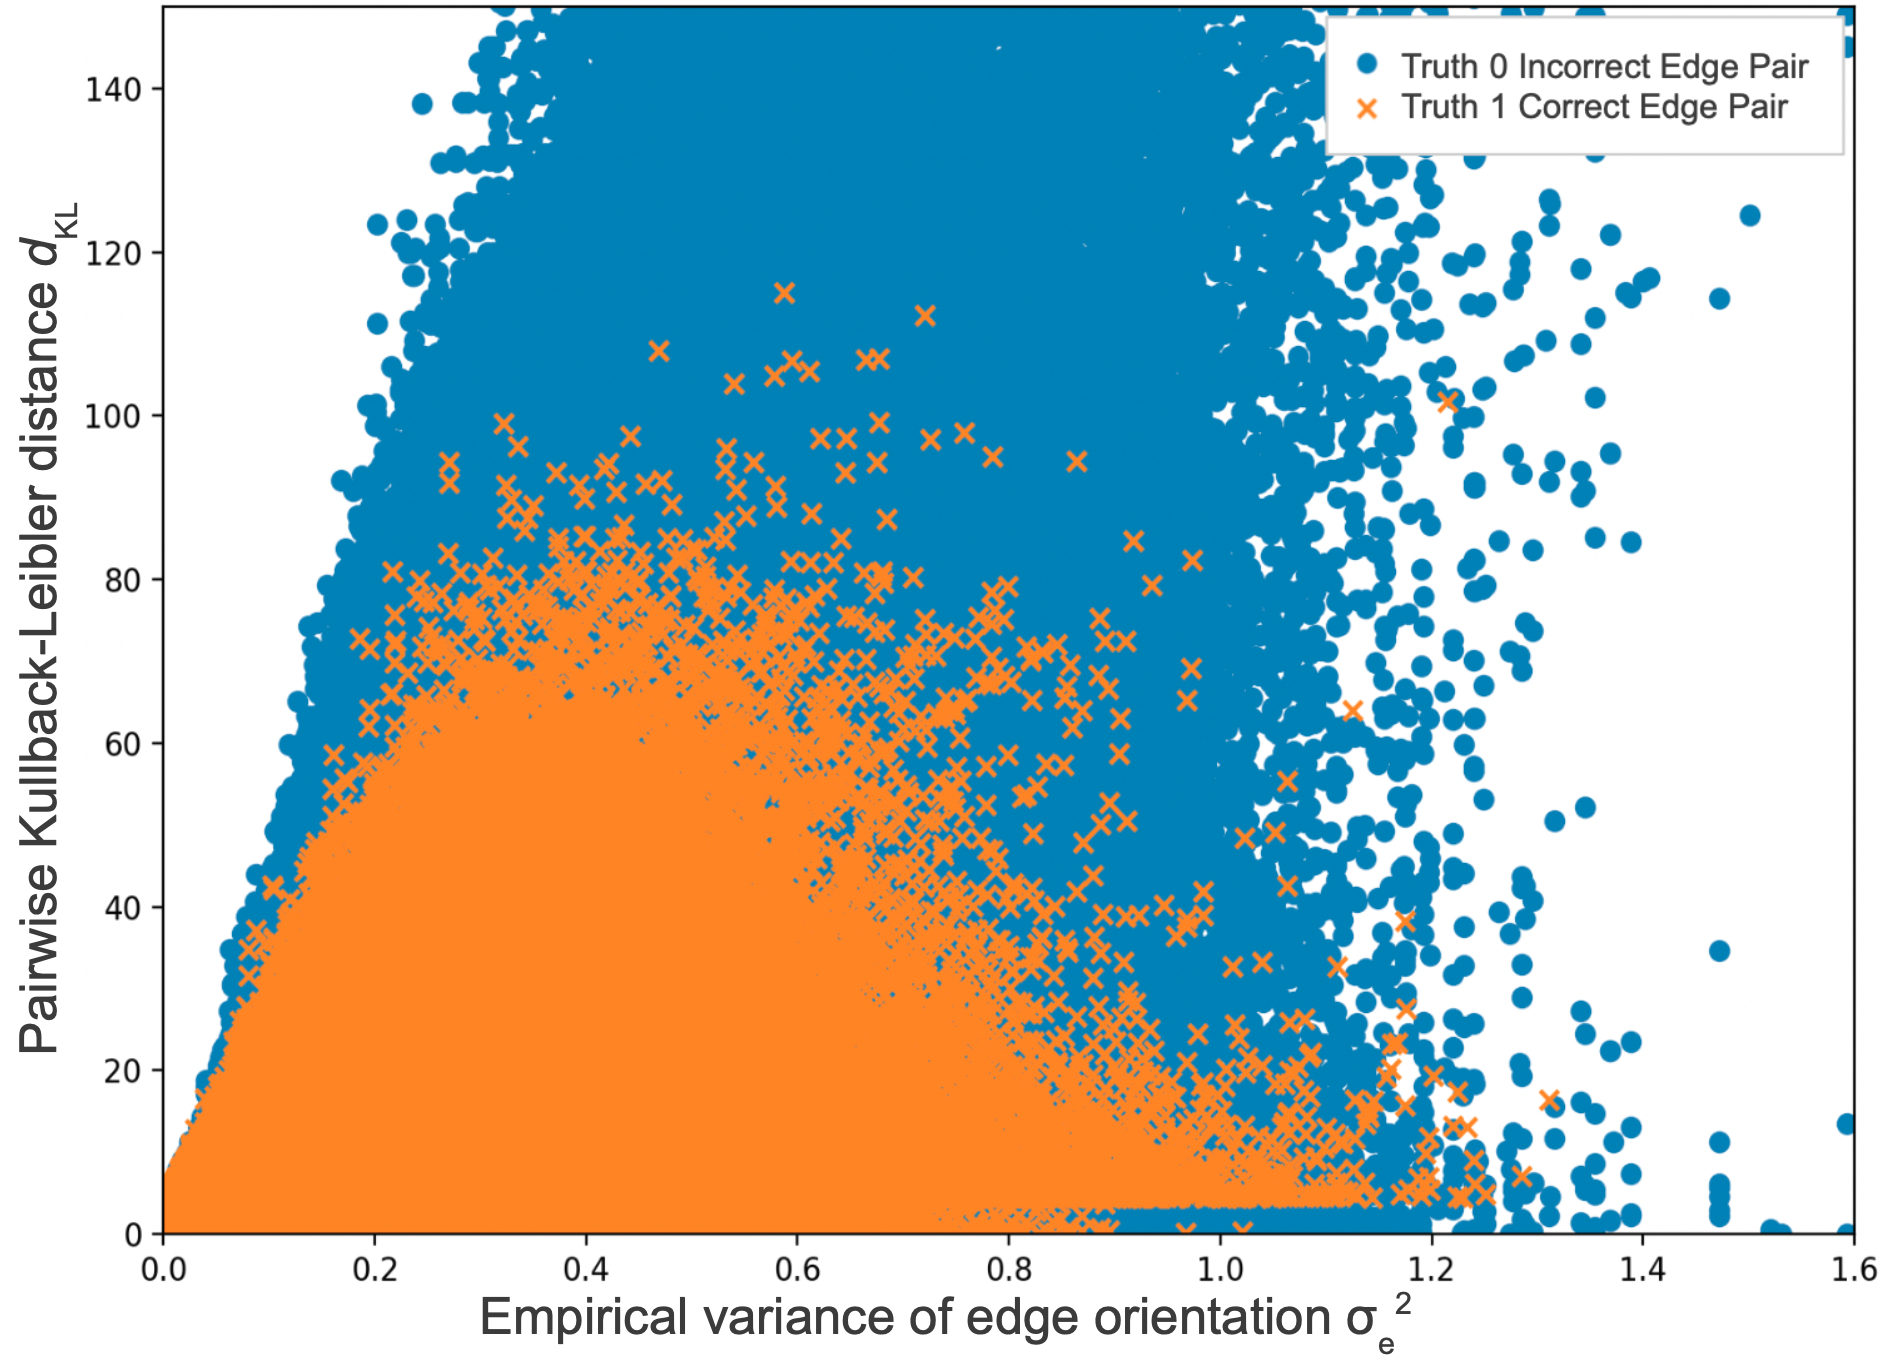
\includegraphics[width=0.88\linewidth]{images/6-trackml/kl-truth-2.png}%
        \label{fig:KL-distance-truth}%
        }%
    \hfill%
    \subfloat[SVM Predictions and Decision Boundary (dotted line)]{%
        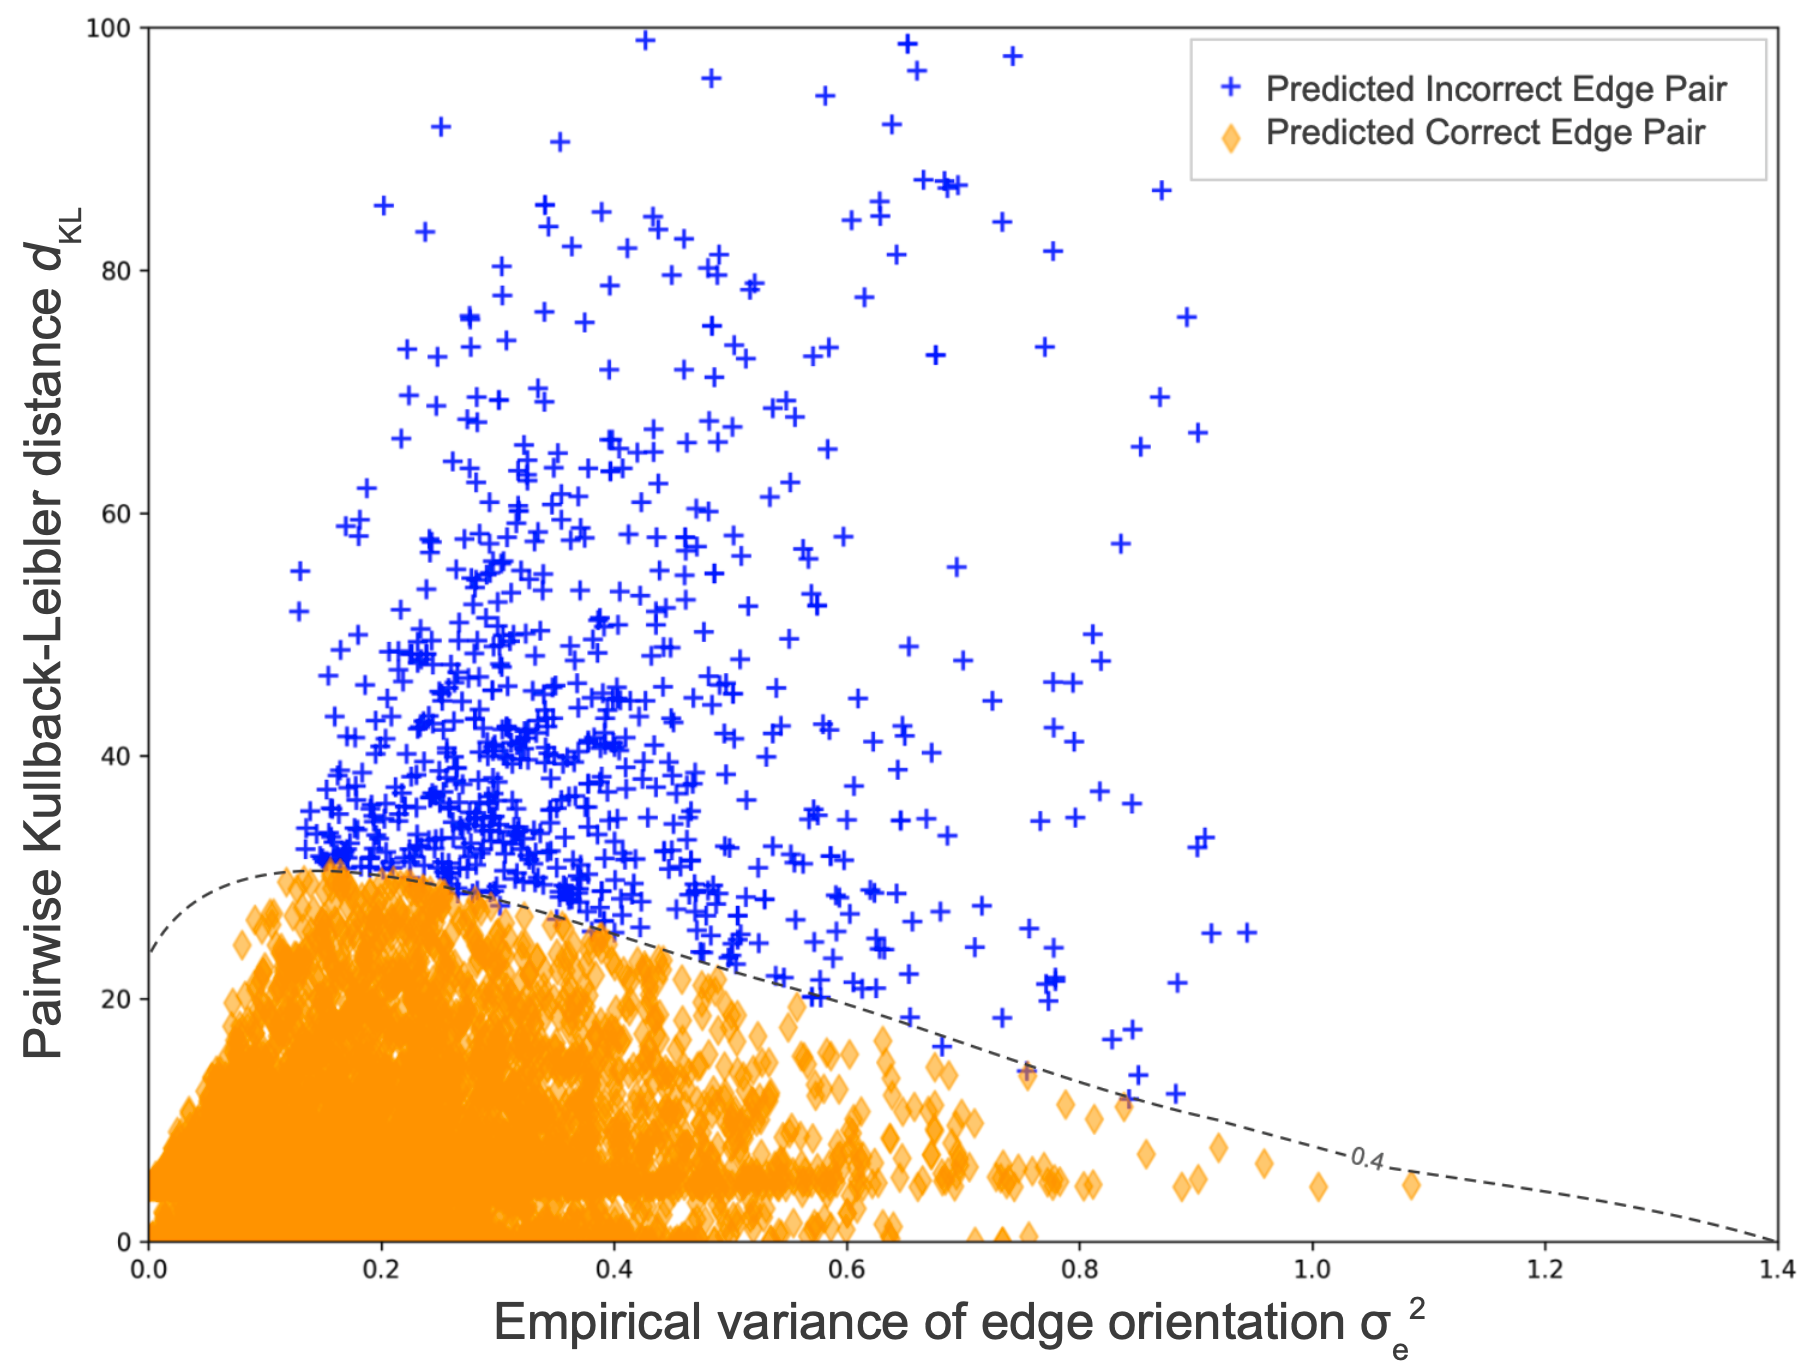
\includegraphics[width=0.88\linewidth]{images/6-trackml/kl-predictions-2.png}%
        \label{fig:KL-distance-predictions}%
        }%
    \caption{SVM classifier training and predictions used to determine the optimal Kullback-Leibler threshold distance, $d_{KL}$, between pairwise track states $X_{ij}$, for a given node with a variance of edge orientation $\sigma_e$. The dotted line in b) represents the threshold value of 0.4 when adjusting SVM predictions in order to yield a TPR of 95\%. For a given pair of edge connections with a common node, truth 1 corresponds to all nodes originate from the same truth particle, and truth 0 corresponds to otherwise.}
    \label{fig:KL-distance}
\end{figure}












\newpage
\section{Extrapolation and Track Extraction}
\label{chapter-6-extrapolation-track-extraction}

\subsection{Overview of KF Implementation}
\label{chapter-6-overview-of-kf}

State extrapolation and track extraction are handled independently for the $x$-$y$ and $r$-$z$ planes, with each stage using a separate KF. Consequently, there are four individual implementations of the KF used within this work. The filter parameters are summarized in Tables \ref{tab:kf-instance-variables-xy} and \ref{tab:kf-instance-variables-rz}, including the numerical values used in its initialization. The underlying models used in the extrapolation and track extraction stages are derived in Sections \ref{chapter-6-start-of-derivation} - \ref{chapter-6-end-of-derivation}.



\begin{table}[!htbp]
\caption{Summary of parameters used in the KFs for state extrapolation and track extraction for the $x$-$y$ plane. The numerical values used in the programmatic implementation to initialize the KFs are also summarized here. Section \ref{chapter-6-start-of-derivation} and \ref{chapter-6-derivation-part-2} provide derivations of the KF models used for the $x$-$y$ plane.}
\begin{center}

\begin{threeparttable}

\begin{tabular}{lccc}
\toprule
& \multicolumn{3}{c}{Parameter Implementation for $x$-$y$ Plane} \\
Variable Description & Symbol  & Extrapolation  & Track Extraction  \\
\hline
\rule{0pt}{3ex}%

Filter State Estimate
& $\hat{x}_{xy}$
& $\tilde{X}_{xy}$
& $\begin{bmatrix} m'_{xy} & \tau'_{xy} & w_{ou} \end{bmatrix}^{T}$
\\
\rule{0pt}{6ex}%

Filter State Covariance
& $\hat{P}_{xy}$ 
& $\tilde{C}_{xy}$ 
& $\begin{bmatrix} \sigma_{xy}^2 & 0 & 0 
                   \\ 0 & \sigma_{\tau_{xy}}^2 & 0 
                    \\ 0 & 0 & \sigma_{w_{ou}}^2 \end{bmatrix}$
\\
\rule{0pt}{4ex}%

% Transition Jacobian
% & $\hat{F}_{xy}$ 
% & $\begin{bmatrix} 
%         \frac{\partial a'}{\partial a} & \frac{\partial a'}{\partial b} & \frac{\partial a'}{\partial c} \\ 
        
%         \frac{\partial b'}{\partial a} & \frac{\partial b'}{\partial b} & \frac{\partial b'}{\partial c} \\
        
%         \frac{\partial c'}{\partial a} & \frac{\partial c'}{\partial b} & \frac{\partial c'}{\partial c} \\
%         \end{bmatrix}$
% & $\begin{bmatrix} 1 & dx' & g_1 \\ 0 & 1 & f_1 \\ 0 & 0 & e_1 \end{bmatrix} $
% \\
% \rule{0pt}{3ex}%


Measurement Function
& $\hat{H}_{xy}$ 
& $[0 \quad 0 \quad 1]$
& $[1 \quad 0 \quad 0]$
% & \multicolumn{2}{c}{$[0 \quad 0 \quad 1]$}
\\
\rule{0pt}{3ex}%

Measurement Uncertainty
& $\hat{R}_{xy}$ 
& $\sigma_{xy}^{2}$
& $\sigma_{xy}^{2}$
% & \multicolumn{2}{c}{$\sigma_{xy}^{2}$}
\\
% \rule{0pt}{6ex}%

% Process Noise
% & $\hat{Q}_{xy}$ 
% &  $\begin{bmatrix} 0 & 0 & 0 \\ 
%                     0 & \sigma_{ms}^2 & 0 \\
%                     0 & 0 & 0 \end{bmatrix}$ 
% & $\begin{bmatrix} Q_{00} & Q_{01} & Q_{02} \\  Q_{01} & Q_{11} & Q_{12} \\ Q_{02} & Q_{12} & Q_{22} \end{bmatrix} $ 
% \\


\bottomrule

% & & & Numerical Value \\
\multicolumn{2}{l}{Variable Description} 
& Symbol & Numerical Value  \\
\hline


\multicolumn{2}{l}{Measurement of Starting Node} 
& $m'_{xy}$ & Measured \\

\multicolumn{2}{l}{Initial Estimate of Track Inclination} 
& $\tau^{'}_{xy}$ & 0 rad \\

\multicolumn{2}{l}{Initial Estimate of Integrated OU\tnote{*}}
& $w_{ou}$ & 0 mm$^{-1}$ \\

\multicolumn{2}{l}{Error due to measurement in $x$-$y$ plane} 
& $\sigma_{xy}$ & 0.3 mm \\

\multicolumn{2}{l}{Initial Estimate of Error in $\tau^{'}_{xy}$} 
& $\sigma_{\tau^{'}_{xy}}$ & 1 rad \\

\multicolumn{2}{l}{Initial Estimate of Error in $w_{ou}$} 
& $\sigma_{w_{ou}}$ & 1 mm$^{-1}$ \\

\multicolumn{2}{l}{Error due to Multiple Scattering} 
& $\sigma_{ms}$ & Derived \\

\multicolumn{2}{l}{Deterministic Drift in OU Process} 
& $\alpha$ & 0.1 mm$^{-1}$ \\

\multicolumn{2}{l}{Stochastic OU Noise} 
& $\sigma_{ou}$ & $10^{-5}$ mm \\

\bottomrule
\end{tabular}

\begin{tablenotes}\footnotesize
\item[*] OU: Ornstein-Uhlenbeck Process \cite{OU} described in further detail in Section \ref{chapter-6-derivation-part-2}.
\end{tablenotes}

\end{threeparttable}
\end{center}

\label{tab:kf-instance-variables-xy}
\end{table}






% \begin{table}[!t]
\begin{table}[H]
\caption{Summary of parameters used in the KFs for state extrapolation and track extraction for the $r$-$z$ plane. The numerical values used in the programmatic
implementation to initialize the KFs are also summarized here. Section \ref{chapter-6-r-z-plane-impl} and \ref{chapter-6-end-of-derivation} provide derivations of the KF models used for the $r$-$z$ plane.}

\begin{center}
\begin{tabular}{lccc}
\toprule

& \multicolumn{3}{c}{Parameter Implementation for $r$-$z$ Plane} \\
Instance Variable Description & Symbol  & Extrapolation  & Track Extraction  \\
\hline
\rule{0pt}{3ex}%


Filter State Estimate
& $\hat{x}_{rz}$
& $\begin{bmatrix} m_{rz} & \tau_{rz} \end{bmatrix}^{T}$
& $\begin{bmatrix} m_{rz} & \tau_{rz} \end{bmatrix}^{T}$
\\
\rule{0pt}{4ex}%

Filter State Covariance
& $\hat{P}_{rz}$
& $\begin{bmatrix} \sigma_{rz}^2 & 0 \\ 0 & \sigma_{\tau_{rz}}^2 + \sigma_{ms}^2\end{bmatrix}$
& $\begin{bmatrix} \sigma_{rz}^2 & 0 \\ 0 & \sigma_{\Sigma}^2\end{bmatrix}$
\\
\rule{0pt}{4ex}%

% Transition Jacobian
% & $\hat{F}_{rz}$ 
% & \multicolumn{2}{c}{$\begin{bmatrix} 1 & dr \\ 0 & 1 \end{bmatrix}$}
% \\
% \rule{0pt}{3ex}%

Measurement Function
& $\hat{H}_{rz}$ 
& $[1 \quad 0]$
& $[1 \quad 0]$
% & \multicolumn{2}{c}{$[1 \quad 0]$}
\\
\rule{0pt}{3ex}%

Measurement Uncertainty
& $\hat{R}_{rz}$ 
& $\sigma_{rz}^2$
& $\sigma_{rz}^2$
% & \multicolumn{2}{c}{$\sigma_{rz}^2$}
\\
\rule{0pt}{3ex}%

Process Noise
& $\hat{Q}_{rz}$ 
& $\sigma_{ms}^2$
& $\sigma_{ms}^2$
% & \multicolumn{2}{c}{$\sigma_{ms}^2$}
\\  

\bottomrule

\multicolumn{2}{l}{Variable Description} 
& Symbol & Numerical Value  \\
\hline

\multicolumn{2}{l}{Measurement of Starting Node} 
& $m_{rz}$ & Measured \\

\multicolumn{2}{l}{Initial Estimate of Track Inclination} 
& $\tau_{rz}$ & 0 rad \\

\multicolumn{2}{l}{Error in Track Inclination $\tau_{rz}$} 
& $\sigma_{\tau_{rz}}$ & Derived \\

\multicolumn{2}{l}{Error in Measurement in the $r$-$z$ Plane} 
& $\sigma_{rz}$ & 0.4 mm, 0.6 mm  \\

\multicolumn{2}{l}{Error due to Multiple Scattering} 
& $\sigma_{ms}$ & Derived \\

\multicolumn{2}{l}{Initial Estimate of Error in $\tau_{rz}$} 
& $\sigma_{\Sigma}$ & 1 rad \\

              

\bottomrule

\end{tabular}
\end{center}
\label{tab:kf-instance-variables-rz}
\end{table}


%The initial estimate of the error in $\tau_{rz}$, $\sigma_{\Sigma}$, represents the error due to track inclination as well as the error due to multiple scattering. Upon initialization of the KF, this information is unknown and hence set to a large initial error.






%\newpage
%\clearpage
\subsection{Parabolic Extrapolation Model}
\label{chapter-6-start-of-derivation}



Given the non-uniformity of the magnetic field in the solenoid, the particle trajectory can be modelled as a parabola in the transverse $x$-$y$ plane. In general, assuming a parabolic model where the track goes through the global origin O, the radius and hence the curvature of the track are uniquely defined. As illustrated by Figure \ref{fig:trackml-parabolic-extrapolation-model-xy}, the parabolic model connects the global origin O to node A, in the local coordinate system of node A given by axis $(X_A, Y_A)$.

\begin{figure}[htbp]
    \centering
    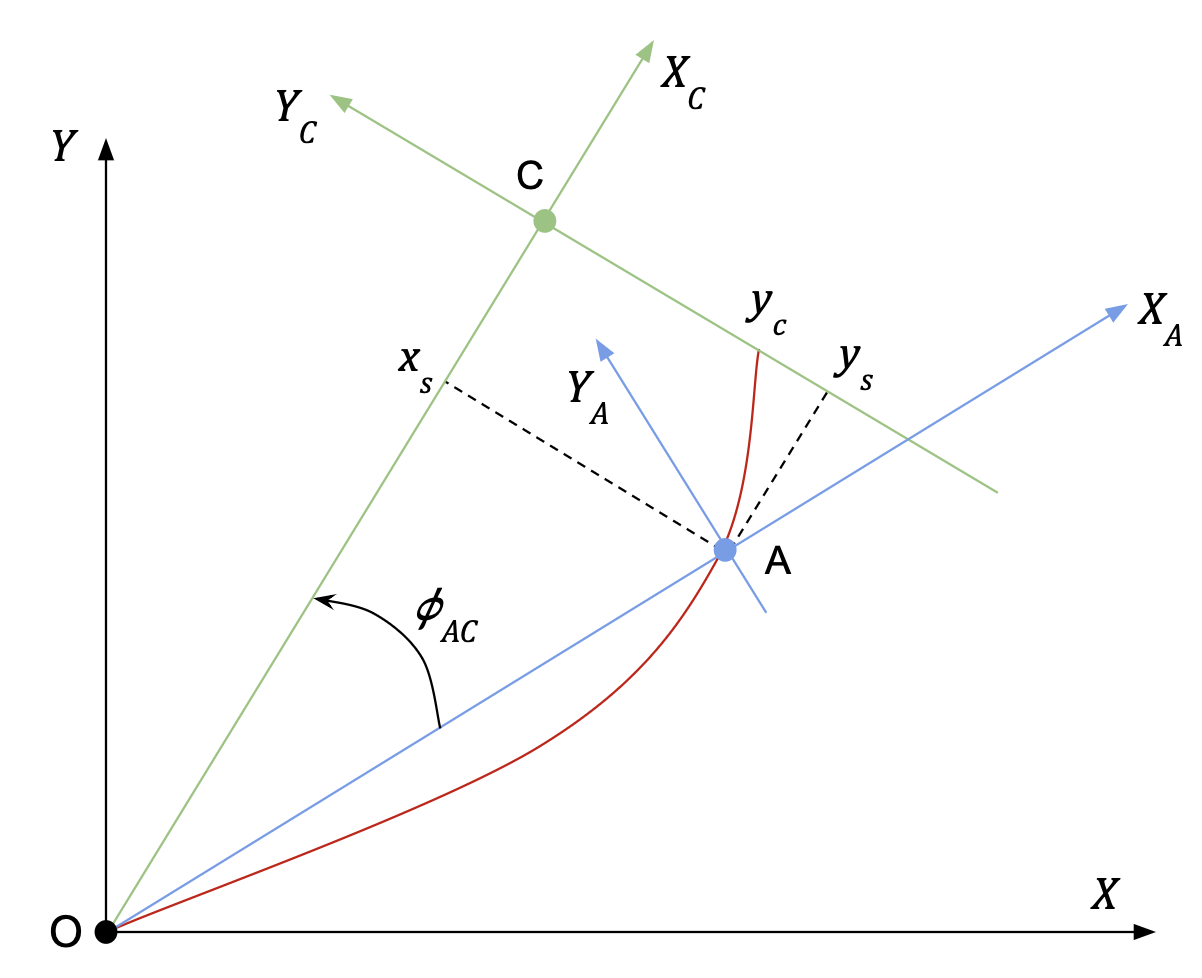
\includegraphics[width=0.65\textwidth]{images/6-trackml/extrapolation-model-xy-trackml-2.png}
    \caption{Illustration of the parabolic extrapolation model used from starting node A and to target node C. The angle of rotation between node A and node C is given by $\phi_{AC}$. The parabola (red) connects the global origin O to node A.}
    \label{fig:trackml-parabolic-extrapolation-model-xy}%
\end{figure}

The parabola has known parameters, $\{a, b, c\}$, derived during previous stages of the algorithm and can be represented in parametric form local to node A, given by Eqs \eqref{eqn:parabolic-equations-parametric}.

\begin{equation}
\begin{aligned}
y_A(u) = au^{2} + bu + c \\
x_A(u) = u
\end{aligned}
\label{eqn:parabolic-equations-parametric}
\end{equation}


%which has a changing curvature. 
%A parabolic model for state extrapolation is used for the transverse $x$-$y$ plane. 

The target node for state extrapolation is node C, which has its own local coordinate system given by axis $(X_C, Y_C)$, and is also described by a parabola. In parametric form, the parabola at node C is given by Eqs \eqref{eqn:parabolic-equations-parametric-nodeC}.

\begin{equation}
\begin{aligned}
y_C(v) = a'v^{2} + b'v + c' \\
x_C(v) = v
\end{aligned}
\label{eqn:parabolic-equations-parametric-nodeC}
\end{equation}

where $\{a', b', c' \}$ are the parabolic parameters in the local coordinate system of node C. The transformation from the local coordinate system of node A to the coordinate system local to node C is given by Eqs \eqref{eqn:rotation-parabolic-linear-algebra}. First a rotation is applied, through angle $\phi_{AC}$ describing the global angle between node A and node C, followed by a translation adding the corresponding shifts $x_s$ and $y_s$.

\begin{equation}
\begin{aligned}
x_C = x_s + u\cos(\phi_{AC}) + (au^2 + bu + c)\sin(\phi_{AC}) \\
y_C = y_s - u\sin(\phi_{AC}) + (au^2 + bu + c)\cos(\phi_{AC})
\end{aligned}
\label{eqn:rotation-parabolic-linear-algebra}
\end{equation}

% the extrapolation ends when this condition is met (target condition

The extrapolation ends when $x_{C}(u) = 0$, as can be seen in Figure \ref{fig:trackml-parabolic-extrapolation-model-xy} when the parabola crosses the $Y_C$ axis. This condition forms a quadratic equation in $u$, where the solution $u^{*} = u(a, b, c)$. Using parametric derivatives, the parabolic parameters $\{a’, b’, c’ \}$ in the coordinate system of the target node, C, can be derived in terms of parabolic parameters $\{a, b, c \}$ in the coordinate system of the starting node A, at the boundary condition $x_{C}(u) = 0$. The Jacobian, $\hat{F}_{xy}$, is then calculated by differentiation of the formulas for $\{a’, b’, c’ \}$ with respect to initial parameters $\{a, b, c \}$, given by Eq \eqref{eqn:transition-jacobian-F-kf-extrapolation-xy}.  

% quadratic equation in s, where the solution s* is a function of the parabolic parameters local to node A. We then have a function s* as a function of a, b, c


\begin{equation}
\hat{F}_{xy} = \begin{bmatrix} 
        \frac{\partial a'}{\partial a} & \frac{\partial a'}{\partial b} & \frac{\partial a'}{\partial c} \\ 
        
        \frac{\partial b'}{\partial a} & \frac{\partial b'}{\partial b} & \frac{\partial b'}{\partial c} \\
        
        \frac{\partial c'}{\partial a} & \frac{\partial c'}{\partial b} & \frac{\partial c'}{\partial c} \\
        \end{bmatrix} 
\label{eqn:transition-jacobian-F-kf-extrapolation-xy}
\end{equation}


The extrapolated track state, $\tilde{X}_{xy}$, and extrapolated covariance, $\tilde{C}_{xy}$, are calculated using $\hat{F}_{xy}$ and Eqs \eqref{eqn:extrapolation}, where the process noise, $\hat{Q}_{xy}$, is given by Eq \eqref{eqn:process-noise-Q-extrapolation-xy}.

\begin{equation}
\hat{Q}_{xy} = \begin{bmatrix} 
                0 & 0 & 0 \\ 
                0 & \sigma_{ms}^2 & 0 \\
                0 & 0 & 0 \end{bmatrix} 
\label{eqn:process-noise-Q-extrapolation-xy}
\end{equation}

The residual, $r$, between the projection of the extrapolated state and the measurement at node C is calculated using Eq \eqref{eqn:residual-trackml-xy}

\begin{equation}
r = m_C - \hat{H}_{xy} \tilde{X}
\label{eqn:residual-trackml-xy}
\end{equation}

where $\hat{H}_{xy} = [0, 0, 1]$ and $m_C$ is the $y$-coordinate of node C in its local coordinate system, hence $m_C = 0$. The covariance of the residual, $V$, is given by Eq \eqref{eqn:covariance-of-residual-trackml-xy}

\begin{equation}
{V} = \hat{H}_{xy} \widetilde{C} \hat{H}^{T}_{xy} + \sigma_{xy}^{2}
\label{eqn:covariance-of-residual-trackml-xy}
\end{equation}

The corresponding Mahalanobis distance, $\Delta \chi^{2}$, is given by Eq \eqref{eqn:mahalanobis-distance-trackml-xy}, and the distributions can be seen in Figure \ref{fig:mahalanobis-threshold-trackml-xy}.

\begin{equation}
\Delta \chi^{2} = r^{T} {V}^{-1} r
\label{eqn:mahalanobis-distance-trackml-xy}
\end{equation}




\begin{figure}[htbp!] 
    \centering
    \subfloat[]{%
        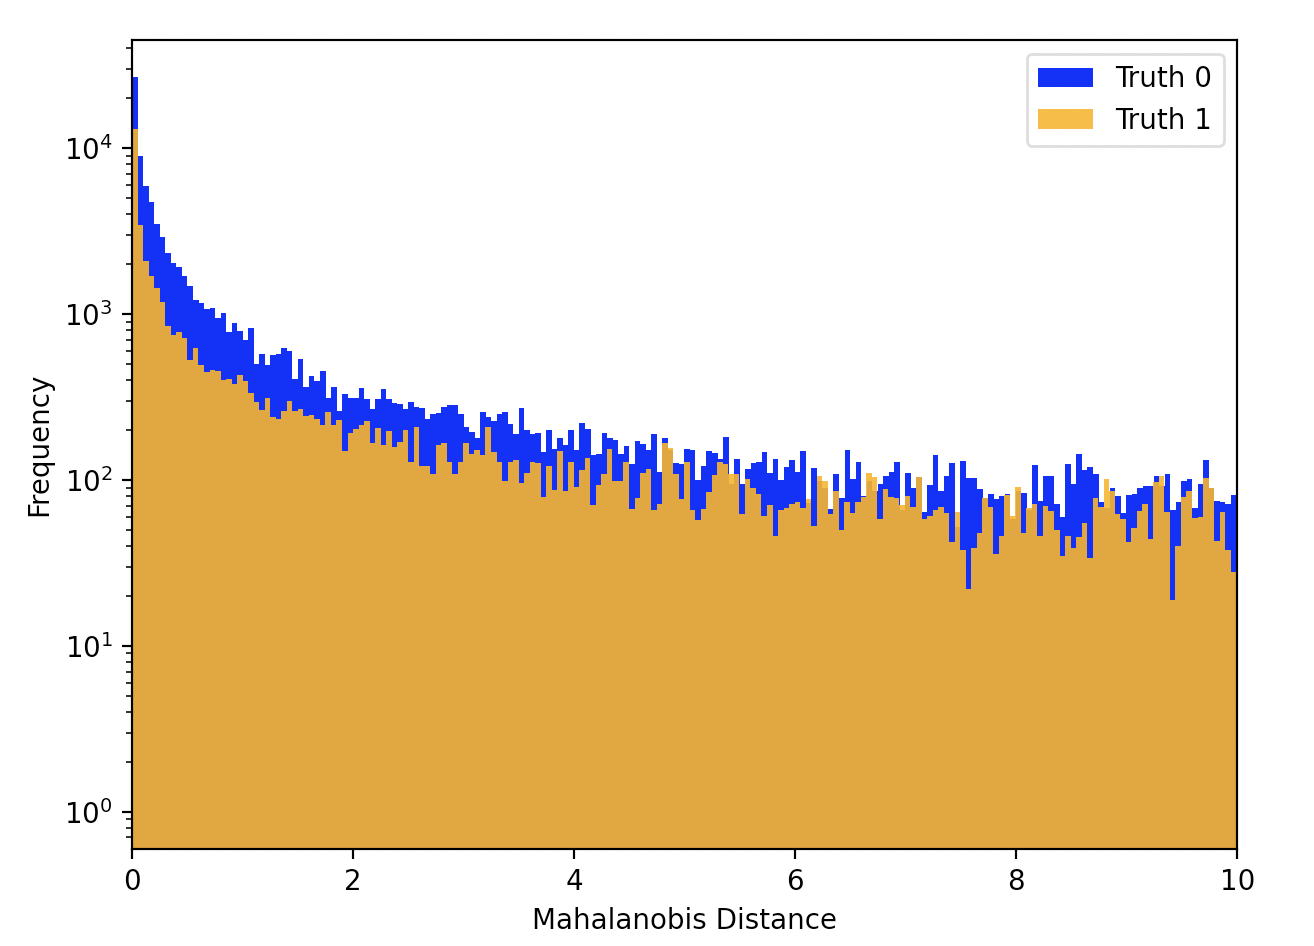
\includegraphics[width=0.85\textwidth]{images/6-trackml/mahalanobis-threshold-trackml-xy-2.png}%
        \label{fig:chi2-distance-trackml-xy-1}%
        }%
    \hfill%
    \subfloat[]{%
        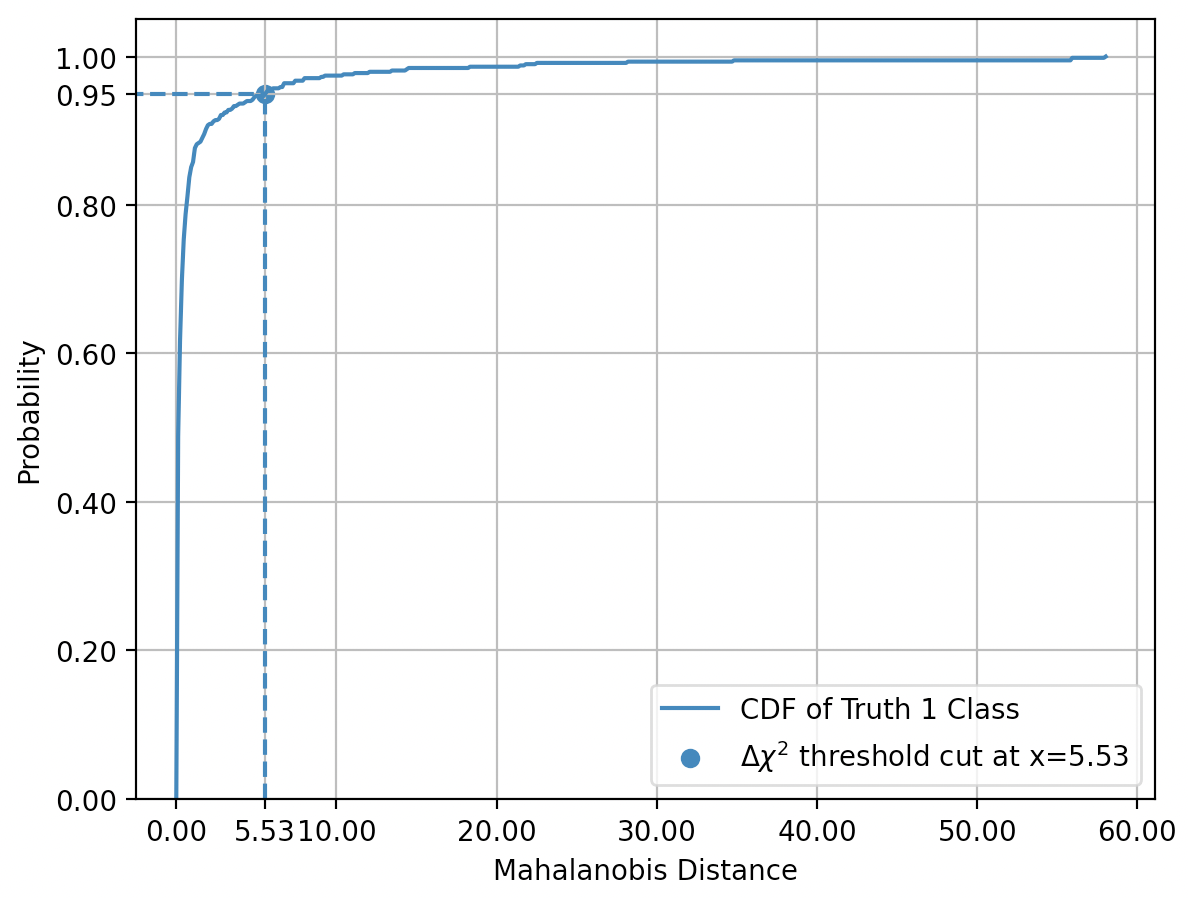
\includegraphics[width=0.8\textwidth]{images/6-trackml/mahalanobis-threshold-trackml-xy-cumulative.png}%
        \label{fig:chi2-distance-trackml-xy-2}%
        }%
    \caption{Mahalanobis distance, $\Delta \chi^{2}$, computed between the projected state and the measurement at each node for the GNN algorithm applied to the TrackML model during state extrapolation in the $x$-$y$ plane. a) Probability distribution for both classes. Truth 1 shows the distribution where the truth particle originating from the extrapolated state and the truth particle originating from the measurement are the same, and truth 0 otherwise. b) Cumulative probability distribution of truth 1 class, where the threshold cut, $d_{\chi}$ = 5.53, was determined in order to provide 95\% efficiency on selecting the truth 1 class.}
    \label{fig:mahalanobis-threshold-trackml-xy}
\end{figure}



A threshold cut, $d_{\chi}$ = 5.53, was determined using the cumulative distribution function shown in Figure \ref{fig:chi2-distance-trackml-xy-2}, in order to provide 95\% efficiency on selecting the truth 1 class. Therefore, if $\Delta \chi^{2} < d_{\chi}$, then $\tilde{X}$ is fully extrapolated to its neighbour node using the KF update. The KF for state extrapolation is initialised with the Jacobian in Eq \eqref{eqn:transition-jacobian-F-kf-extrapolation-xy} and process noise in Eq \eqref{eqn:process-noise-Q-extrapolation-xy}.

One can assume a uniform magnetic field during the extrapolation of track states in the $x$-$y$ plane across between adjacent layers, such that the particle trajectory remains as a parabola. However, this assumption cannot be made during the track fitting stage (see Section \ref{chapter-6-derivation-part-2} for further information). 








\clearpage
\subsection{Kalman Filter Track Extraction in Transverse Plane}
\label{chapter-6-derivation-part-2}
%The KF track fit is applied simultaneously in both the $x$-$y$ and $r$-$z$ planes, in order to assess the quality of the fit using both models. In comparison to the KF used for state extrapolation (Section \ref{kf-for-extrp-chapter-6}), the KF for track fitting considers the entire chain of track segments making up a track candidate. Therefore, there will be a non-zero process noise, $Q$, present in both $x$-$y$ and $r$-$z$ planes.

\subsubsection{Rotated Coordinate System}

The KF works in a rotated coordinate system, whereby the first track segment in the chain of segments representing a track candidate is rotated to be parallel to the global $x$-axis. This decision is made to avoid singularities from occurring in calculations of gradients, for near vertical tracks. The rotated coordinate system is denoted by $(x', y')$, not to be confused with the global coordinate system $(x, y)$. The new $x$-axis, $x'$, is parallel to the first track segment and the new $y$-axis, $y'$, describes the track deviation from the straight line.

\subsubsection{Motivation for Ornstein-Uhlenbeck Process Noise}

As opposed to the parabolic model used in Section \ref{chapter-6-start-of-derivation}, whereby the magnetic field was assumed to be uniform across the extrapolation distance between two connected nodes, one cannot make the same assumption during the track fitting and extraction stage. In this instance, one must consider the influence of the magnetic field, as the region of interest is now much larger when considering an entire chain of track segments spanning multiple detector layers, compared with one track segment alone. The effect of the magnetic field is not negligible across multiple detector layers and is an important aspect to incorporate. In principle, the parabolic model may be used for track fitting in the KF. However, this would introduce many additional calculations when transforming between local to global coordinate systems (and vice versa), as well as a higher degree of complexity in the filter during the recording of many different parameters. Rather it was investigated if a simpler approach could be taken, using a lower dimensionality model.

As the track bends in a particular direction, dependent on the charge of the particle, the magnetic field creates a systematic effect on the track direction and hence a near-constant drift in the azimuthal angle from the $x$-axis, $\phi$. Statistically, such a situation can be described as a correlated noise which affects the track direction. For example consider a random walk; there exists some systematic effect on the evolution of a variable, as well as a stochastic component. In financial mathematics, stochastic differential equations are widely used to model the evolution of financial interest rates or asset prices, with a degree of volatility \cite{financial-maths-sde}. The daily movements of stocks and shares can resemble a random walk or a path taken by a Brownian motion (referred to as the Wiener process). 

In this setting, the low levels of curvature in particle trajectories can be described by a linear transition model with an additive random noise. This is described by the Ornstein-Uhlenbeck (OU) process \cite{OU}. Using the OU process, the track direction evolves stochastically according to a deterministic drift parameter, $\alpha$, and stochastic noise, $\sigma_{ou}$. The result is one which can be substituted into the KF as a sophisticated process noise, making the KF track fit three-dimensional. This approach is simple in nature yet highly advantageous; by leveraging the linear model with an addition of a stochastic element, the effect of the magnetic field can be incorporated.


\subsubsection{Filter Implementation}

For a set of $n$ nodes representing a track candidate, the sequential set of measurements are $\{m'_{(n-1)}, ..., m'_1, m'_0, \}$, where $m'_{(n-1)}$ is the measurement of the node with the largest radius, as the track extraction works from the outermost node. The KF is initialised with the following three-dimensional filter state estimate, $\hat{x}_{xy}$, given by Eq \eqref{eqn:kf-track-fit-initialised-state-xy}.


\begin{equation}
\hat{x}_{xy} = \begin{bmatrix} m'_{(n-1)} \\ \tau'_{xy} \\ w_{ou} \end{bmatrix} 
\label{eqn:kf-track-fit-initialised-state-xy}
\end{equation}

where the measurement $m'_{(n-1)}$ is known, $\tau'_{xy}$ is the track inclination in the $(x', y')$ coordinate system initialized to zero and $w_{ou}$ is the integrated OU parameter, also initialized to zero. The filter covariance matrix, $\hat{P}_{xy}$, is initialized using Eq \eqref{eqn:kf-track-fit-initialised-cov-xy}

\begin{equation}
\hat{P}_{xy} = \begin{bmatrix} \sigma_{xy}^2 & 0 & 0 
                            \\ 0 & \sigma_{\tau^{'}_{xy}}^2 & 0 
                            \\ 0 & 0 & \sigma_{w_{ou}}^2 \end{bmatrix} 
\label{eqn:kf-track-fit-initialised-cov-xy}
\end{equation}

where $\sigma_{\tau^{'}_{xy}}$ is the error in the track inclination, $\tau_{xy}$, and is initialized to 1, and $\sigma_{w_{ou}}$ is the error in the integrated OU parameter, $w_{ou}$, initialized to 1. The state transition Jacobian $\hat{F}_{xy}$ is derived by integration of the OU motion model \cite{OU} and is given by \eqref{eqn:state-transition-jacobian-ou},

\begin{equation}
\hat{F}_{xy} = \begin{bmatrix} 1 & dx' & g_1 \\ 0 & 1 & f_1 \\ 0 & 0 & e_1 \end{bmatrix} 
\label{eqn:state-transition-jacobian-ou}
\end{equation}

where $dx'$ is the difference in $x'$ position of sequential nodes $i$ and $j$ processed in the the KF, $dx' = x'_i - x'_j$, and $e_1$, $f_1$ and $g_1$ are given by the following equations. 

\begin{equation}
e_1 = e^{- \alpha \lvert dx' \rvert}
\label{eqn:e1}
\end{equation}

\begin{equation}
f_1 = \frac{1 - e_1}{\alpha}
\label{eqn:f1}
\end{equation}

\begin{equation}
g_1 = \frac{\lvert dx' \rvert - f_1}{\alpha}
\label{eqn:g1}
\end{equation}

The inverse of the deterministic drift parameter, $\alpha^{-1}$, is proportional to the rate of change of the track azimuthal angle, $\phi$, where $\alpha$ is initialised to 0.1. If $\alpha \rightarrow \infty$ the track model becomes a straight line, however if $\alpha \rightarrow 0$, the model becomes a parabola. The process noise, $\hat{Q}_{xy}$, is derived using the OU motion model \cite{OU} and is given by Eq \eqref{eqn:process-noise-q}, 
 
\begin{equation}
\hat{Q}_{xy} = \begin{bmatrix} Q_{00} & Q_{01} & Q_{02} \\  Q_{01} & Q_{11} & Q_{12} \\ Q_{02} & Q_{12} & Q_{22} \end{bmatrix} 
\label{eqn:process-noise-q}
\end{equation}

where the corresponding matrix elements are given by the following equations.

\begin{equation}
Q_{00} = (dx')^{2} (\sigma_{ms}^{2} + \frac{(dx')^{2} \sigma_{ou}^{2}}{4})
\label{eqn:q00}
\end{equation}


\begin{equation}
Q_{01} = dx'( \sigma_{ms}^2 + Q_{02} )
\label{eqn:q01}
\end{equation}

\begin{equation}
Q_{02} = \frac{1}{2} (dx')^2 \sigma_{ou}^{2}
\label{eqn:q02}
\end{equation}

\begin{equation}
Q_{12} = dx' \sigma_{ou}^{2}
\label{eqn:q12}
\end{equation}

\begin{equation}
Q_{11} = \sigma_{ms}^2 + (dx')^{2} \sigma_{ou}^{2}
\label{eqn:q22}
\end{equation}

\begin{equation}
Q_{22} = \sigma_{ou}^2
\label{eqn:q22}
\end{equation}

The process noise, $\hat{Q}_{xy}$, is implemented with the addition of a non-zero stochastic noise, $\sigma_{ou}$, as well as the non-zero error due to the multiple scattering, $\sigma_{ms}$, derived using Eq \eqref{eqn:computed-multiple-scattering}. This represents the correlated noise and models the track curvature caused by the presence of the magnetic field.














\clearpage
\subsection{Linear Extrapolation Model}
\label{chapter-6-r-z-plane-impl}


Similar to Section \ref{gnn-application-toy-model}, a linear model is used for track state extrapolation in the $r$-$z$ plane, as the particle trajectory follows a near linear path. Each connection is modelled as a straight line, where the state to extrapolate, $x_{rz}$, from node $i$ to neighbour node $j$ consists of the $z$-position at node $i$, $m_i$, and the track inclination to node $j$, $\tau_{ij}$, extracted from the combined track state estimate, $X_{ij}$, described at node $i$. The state to extrapolate, $x_{rz}$, is given by Eq \eqref{eqn:track-state-estimate-rz}.

\begin{equation}
x_{rz} = \begin{bmatrix} m_i \\ \tau_{ij} \end{bmatrix}
\label{eqn:track-state-estimate-rz}
\end{equation}


The corresponding state covariance matrix, $P_{rz}$, is stated in Eq. \eqref{eqn:kf-track-fit-initialised-cov-rz}.  

\begin{equation}
P_{rz} = \begin{bmatrix} \sigma_{rz}^2 & 0 \\ 0 & \sigma_{\tau_{rz}}^2 + \sigma_{ms}^2 \end{bmatrix} 
\label{eqn:kf-track-fit-initialised-cov-rz}
\end{equation}

The magnitude of the uncertainty in the measurement of the $r$-$z$ plane, $\sigma_{rz}$, is dependent on the detector layer where the graph node is situated. For example, for an endcap-located node, the uncertainty in the measurement will be greater than for a barrel-located node, due to the orientation of the detector layer. Therefore, for a node located in the pixel barrel $\sigma_{rz} = 0.4$ mm and for a node located in the pixel endcap $\sigma_{rz} = 0.6$ mm. The derivation of the uncertainty in track inclination, $\sigma_{\tau_{rz}}$, is described in Section \ref{variance-in-inverse-track-inclination}. 

Similar to the procedure described in Section \ref{gnn-application-toy-model}, the state, $x_{rz}$, is projected into the subspace of measurements in the $r$-$z$ plane, where the residual and corresponding Mahalanobis distance, $\Delta \chi_{ij}^{2}$, between the projection and the measurement at each node is calculated. Similar to Section \ref{chapter-6-start-of-derivation}, a threshold distance is determined by using the truth distributions of $\Delta \chi_{ij}^{2}$ in order to provide 95\% efficiency in selection of the truth class 1. 



%\subsection{KF Setup for State Extrapolation}

The extrapolated state, $\widetilde{X}_{ij}$, is calculated by the KF using \eqref{eqn:extrapolation} defined as the linear extrapolation from node $j$ to node $i$. This is described by $m_i = m_j + \tau_j dr$ and $\tau_i = \tau_j$, where $m_i$ and $m_j$ are the $z$-measurements of node $i$ and node $j$ respectively. Therefore, the derived Jacobian, $\hat{F}$, for the KF is given by Eq \eqref{eqn:mc-model-F-rz}.

% Jacobian F is derived by differentation of m_i and t_i equations with respect to initial parameters m_j and t_j

\begin{equation}
\hat{F}_{rz} = \begin{bmatrix} 1 & dr \\ 0 & 1 \end{bmatrix}
\label{eqn:mc-model-F-rz}
\end{equation}

where $dr$ is the difference in radial position of nodes $i$ and $j$, $dr = r_i - r_j$.






\subsection{Kalman Filter Track Extraction in r-z Plane}
\label{chapter-6-end-of-derivation}
% linear KF model, with non-zero process noise Q, following multiple scattering only

The KF for track extraction in the $r$-$z$ plane uses a linear model. For a set of $n$ nodes representing a track candidate, the sequential $z$-measurements are $\{z_{(n-1)}, ..., z_1, z_0, \}$, where $z_{(n-1)}$ is the $z$-measurement of the node with the largest radius, as the filter works from the outermost node. The KF is initialised with the following two-dimensional filter state estimate, $\hat{x}_{rz}$, given by Eq \eqref{eqn:kf-track-fit-initialised-state-rz}.

\begin{equation}
\hat{x}_{rz} = \begin{bmatrix} z_{(n-1)} \\ \tau_{(n-1)} \end{bmatrix} 
\label{eqn:kf-track-fit-initialised-state-rz}
\end{equation}


where the track position measurement, $z_{(n-1)}$, is known and the track inclination, $\tau_{(n-1)}$, is initialized to zero as track inclination information is unknown at the start of the filter. As the magnetic field only influences the transverse $x$-$y$ plane, the process noise, is reduced to the contribution due to multiple scattering only, such that $\hat{Q}_{rz} = \sigma_{ms}^{2}$, where $\sigma_{ms}^{2}$ is derived using Eq \eqref{eqn:computed-multiple-scattering}.





% \subsubsection{Track Extraction}

% As the two KF track fits are simultaneously executed in the $x$-$y$ and $r$-$z$ planes, the corresponding Mahalanobis distances are calculated for each sequential node-pair. The $\chi^2$-statistic is calculated by summing all individual Mahalanobis distances for each track candidate and the corresponding degrees of freedom, $d_f$ is also computed. The p-value corresponding to the track fit is then calculated using the $d_f$ and the $\chi^2$-statistic. If $p > 0.01$ then track is considered a good track candidate and hence extracted from the main graph network.
%---------------------------------------------
%	7. Application & Perform of GNN Algorithm
%---------------------------------------------

\chapter{Application of the GNN Algorithm to the TrackML Model}
\label{chapter-7}

This chapter focuses on the application of the GNN algorithm to the Pixel endcap and Pixel barrel regions of the TrackML detector. This chapter is organised as follows. Section \ref{chapter-7-endcap-results} presents the results of the GNN algorithm applied to the Pixel endcap region of the TrackML detector. The performance of the algorithm is evaluated and track reconstruction efficiency metrics are discussed. Section \ref{chapter-7-outlook} presents preliminary results and challenges faced when applying the GNN algorithm onto the full Pixel detector of the TrackML geometry, including the barrel region. Potential software optimisations and other approaches explored are also discussed, followed by several improvements that would be necessary to implement within the GNN algorithm in order for it to be considered for proper online usage for track reconstruction in particle detectors.



\section{Pixel Endcap Results}
\label{chapter-7-endcap-results}


\subsection{Performance Evaluation on Volume 7}
\label{performance-eval-endcap-vol-7-start}

The GNN algorithm is first applied to volume 7 of the TrackML detector model (see Figure \ref{fig:trackml-detector-image}), by isolating the left Pixel endcap. The geometry in the endcap consists of parallel silicon layers and is the simplest part of the detector to begin reconstruction. An example TrackML simulated event is shown in Figure \ref{fig:trackml-results-endcap-nodes-sim}.

\begin{figure}[htbp!] 
    \centering
    \subfloat[$x$-$y$ plane view]{%
        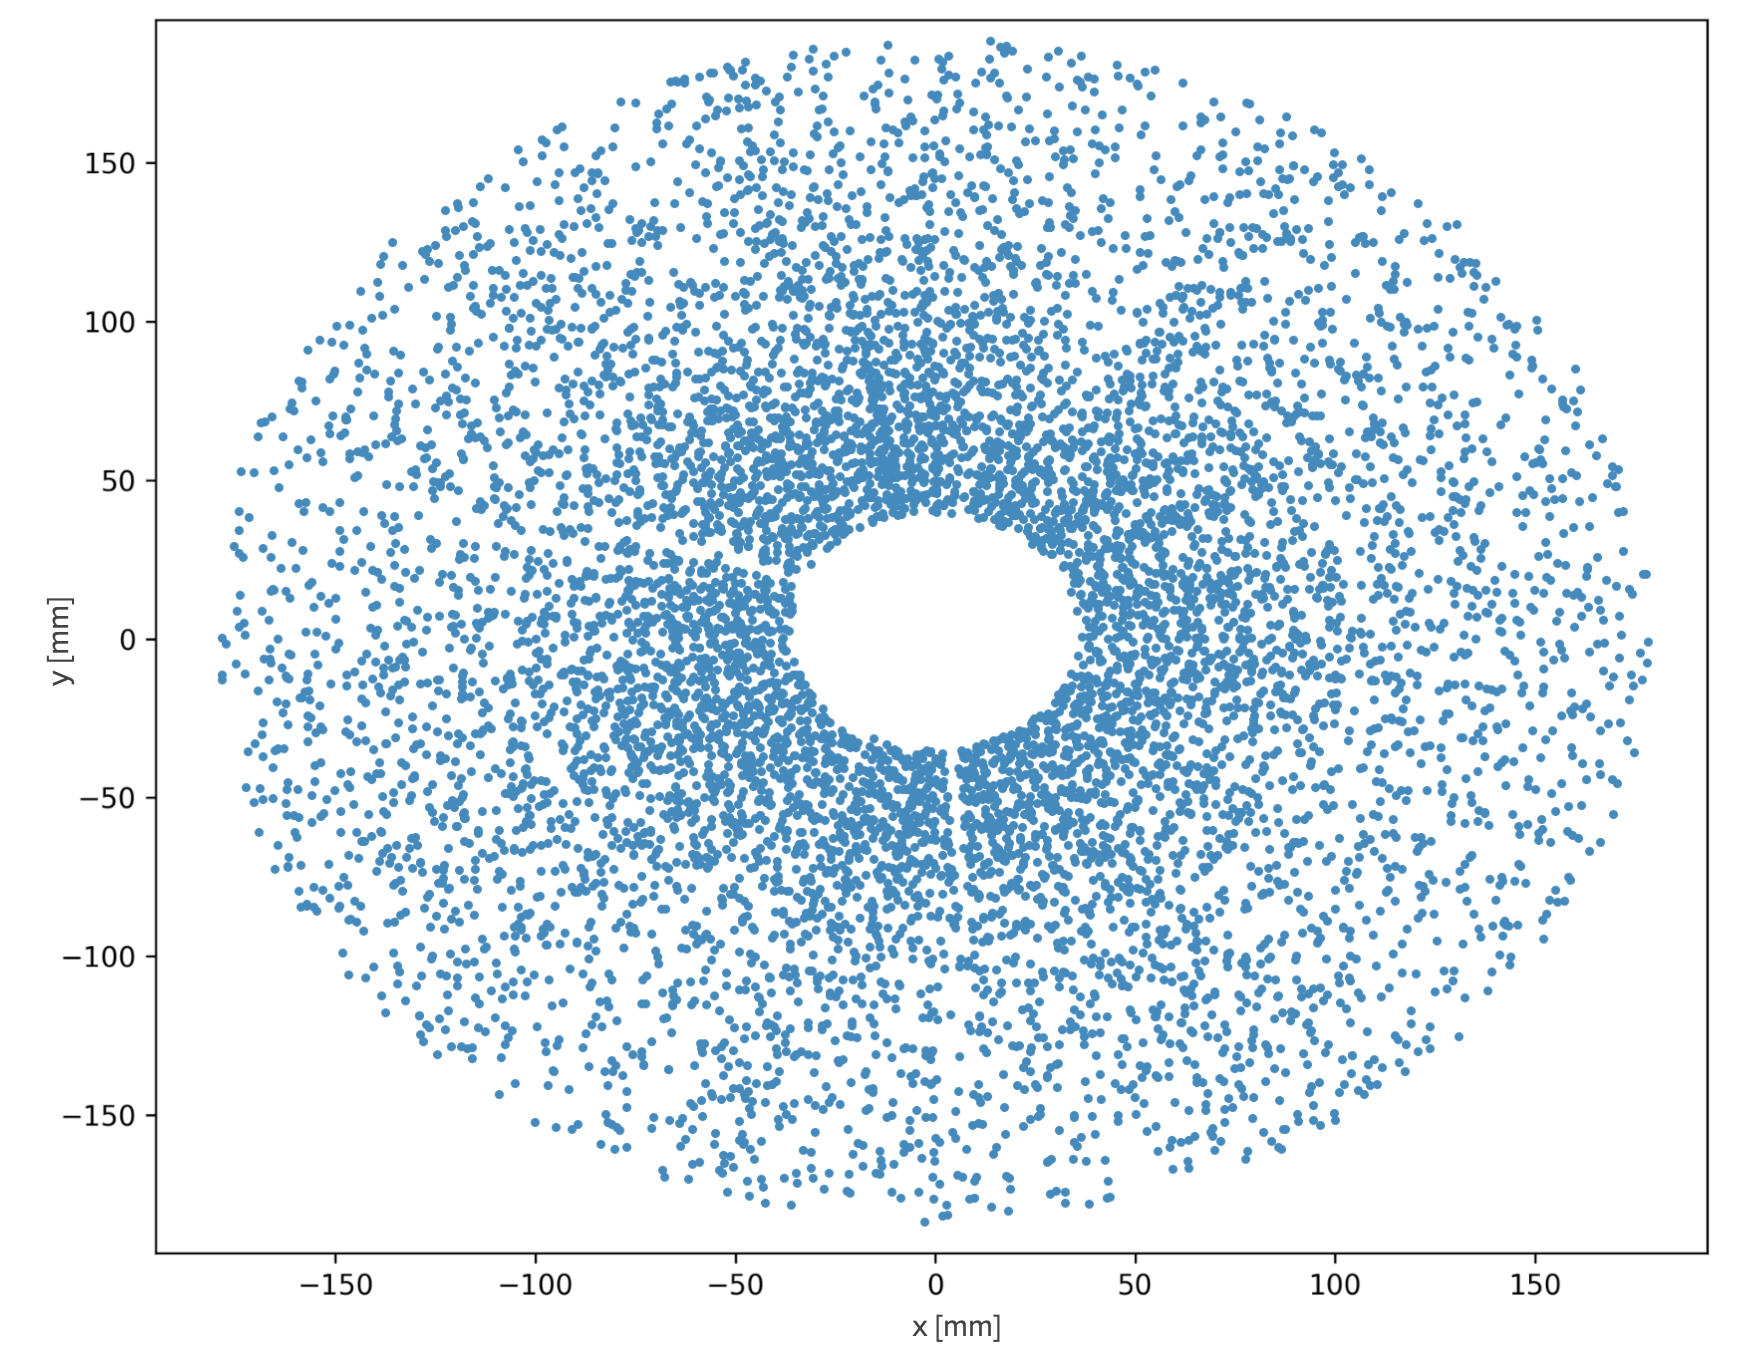
\includegraphics[width=0.50\linewidth]{images/7-results/trackml-endcap-nodes-xy.png}%
        \label{fig:endcap-trackml-sim-xy}%
        }%
    \hfill%
    \subfloat[$r$-$z$ plane view]{%
        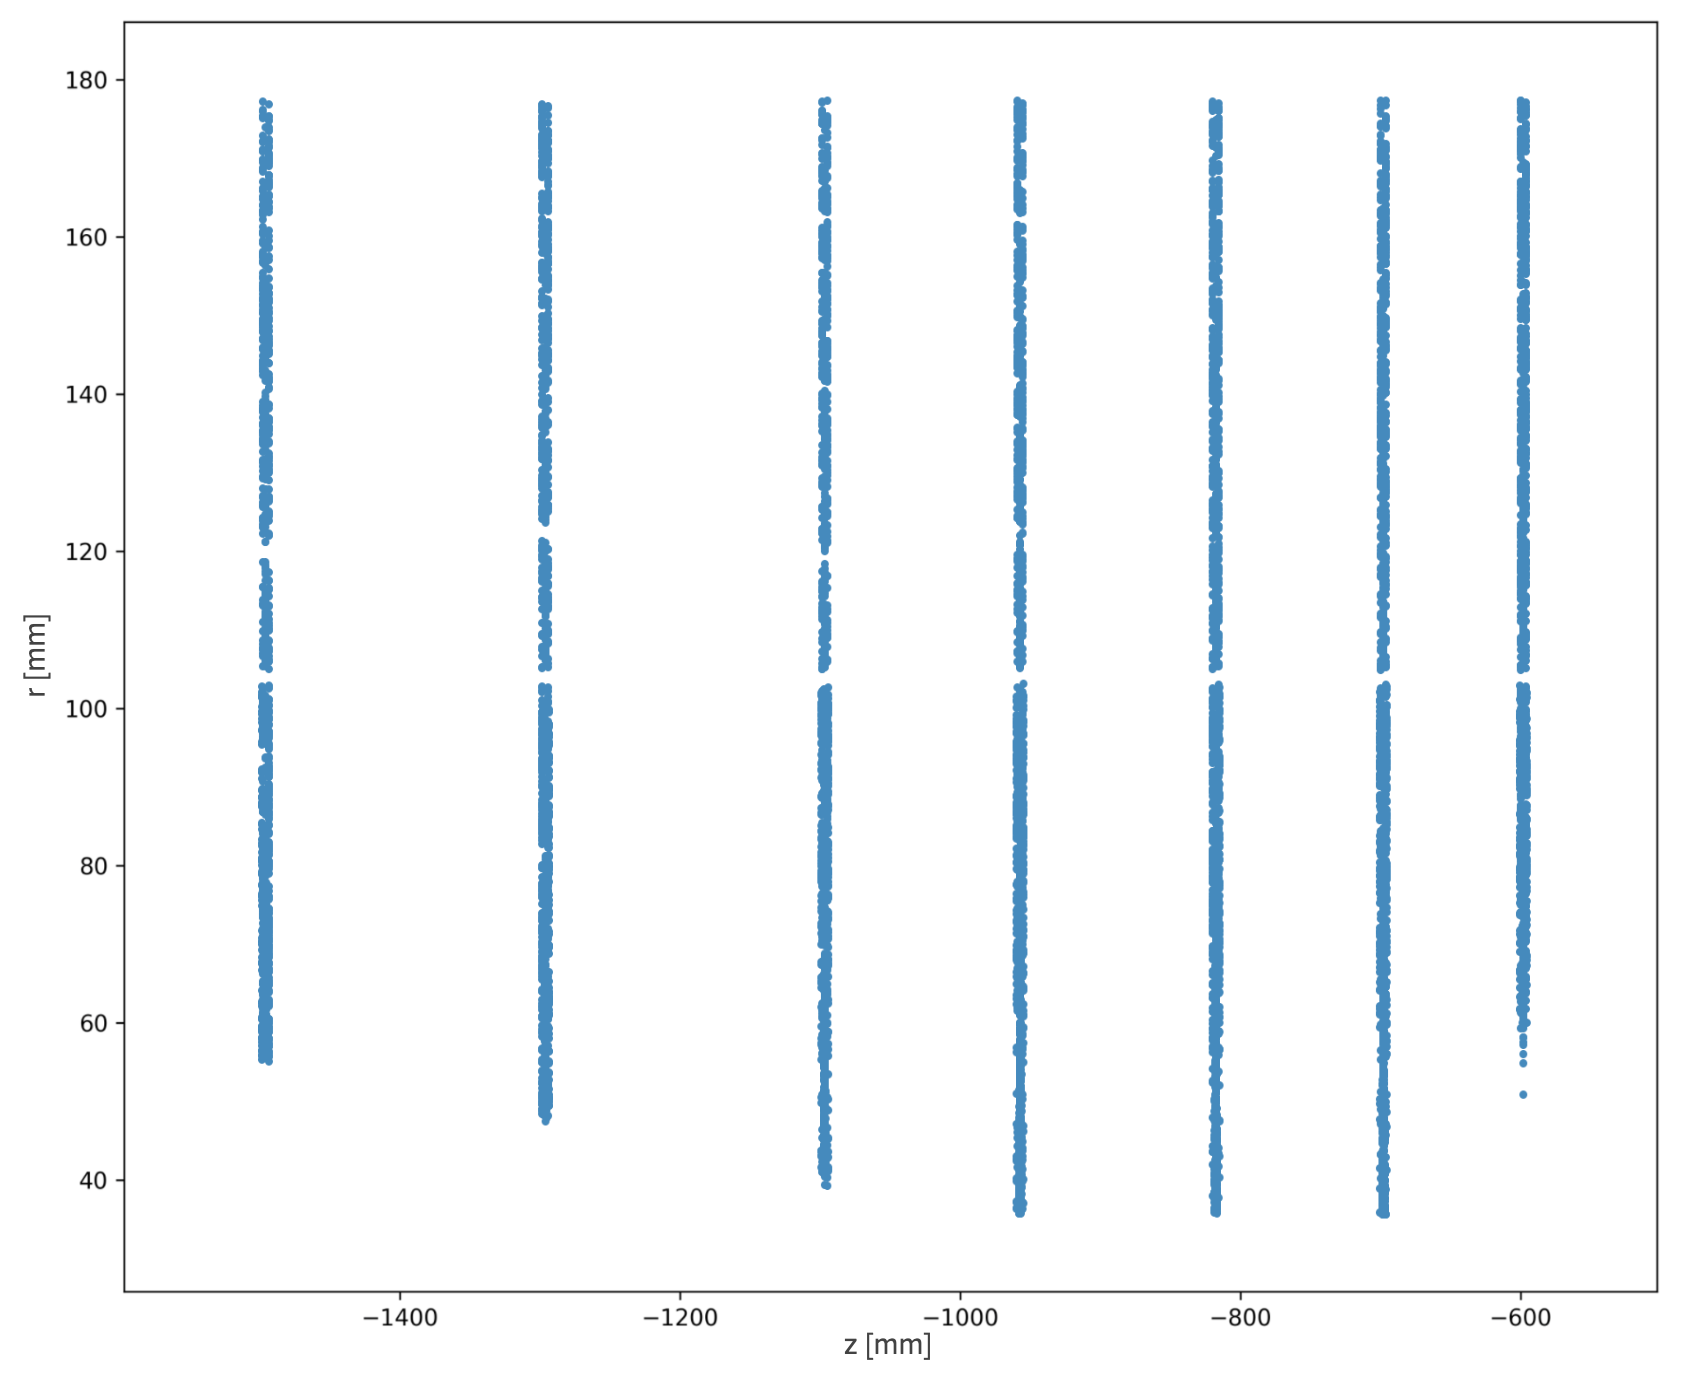
\includegraphics[width=0.48\linewidth]{images/7-results/trackml-endcap-nodes-rz.png}%
        \label{fig:endcap-trackml-sim-rz}%
        }%
    \caption{Event simulation of the TrackML detector isolating volume 7.}
    \label{fig:trackml-results-endcap-nodes-sim}
\end{figure}


The graph network is constructed using 9835 nodes located in volume 7 from a simulated TrackML event and 18,184 predicted edges using the FASTrack algorithm \cite{Dmitry-fasttrack-addtest}, as described in Section \ref{chapter-6-data-prep}. The FASTrack algorithm uses several cuts on track parameters when the graph segments are generated. For this particular test the following cut was used: $p_{\text{T}} \ge 150$ MeV. Using the same generated graph, this cut was then increased to $p_{\text{T}} \ge 1$ GeV in order to investigate the reconstruction efficiency for different levels of curvature. Track state estimates, $X_{ij}$, are constructed using the model as described in Section \ref{constructing-track-states}. Figure \ref{fig:trackml-results-endcap-extracted} illustrates the extracted track candidates post Stage 1 of application of the GNN algorithm, where 1054 track candidates were successfully extracted. Figure \ref{fig:trackml-results-endcap-extracted-v2} shows the extracted track candidates post Stage 2, where a further 265 candidates were extracted.

\begin{figure}[htbp]%
    \centering
    \subfloat[]{{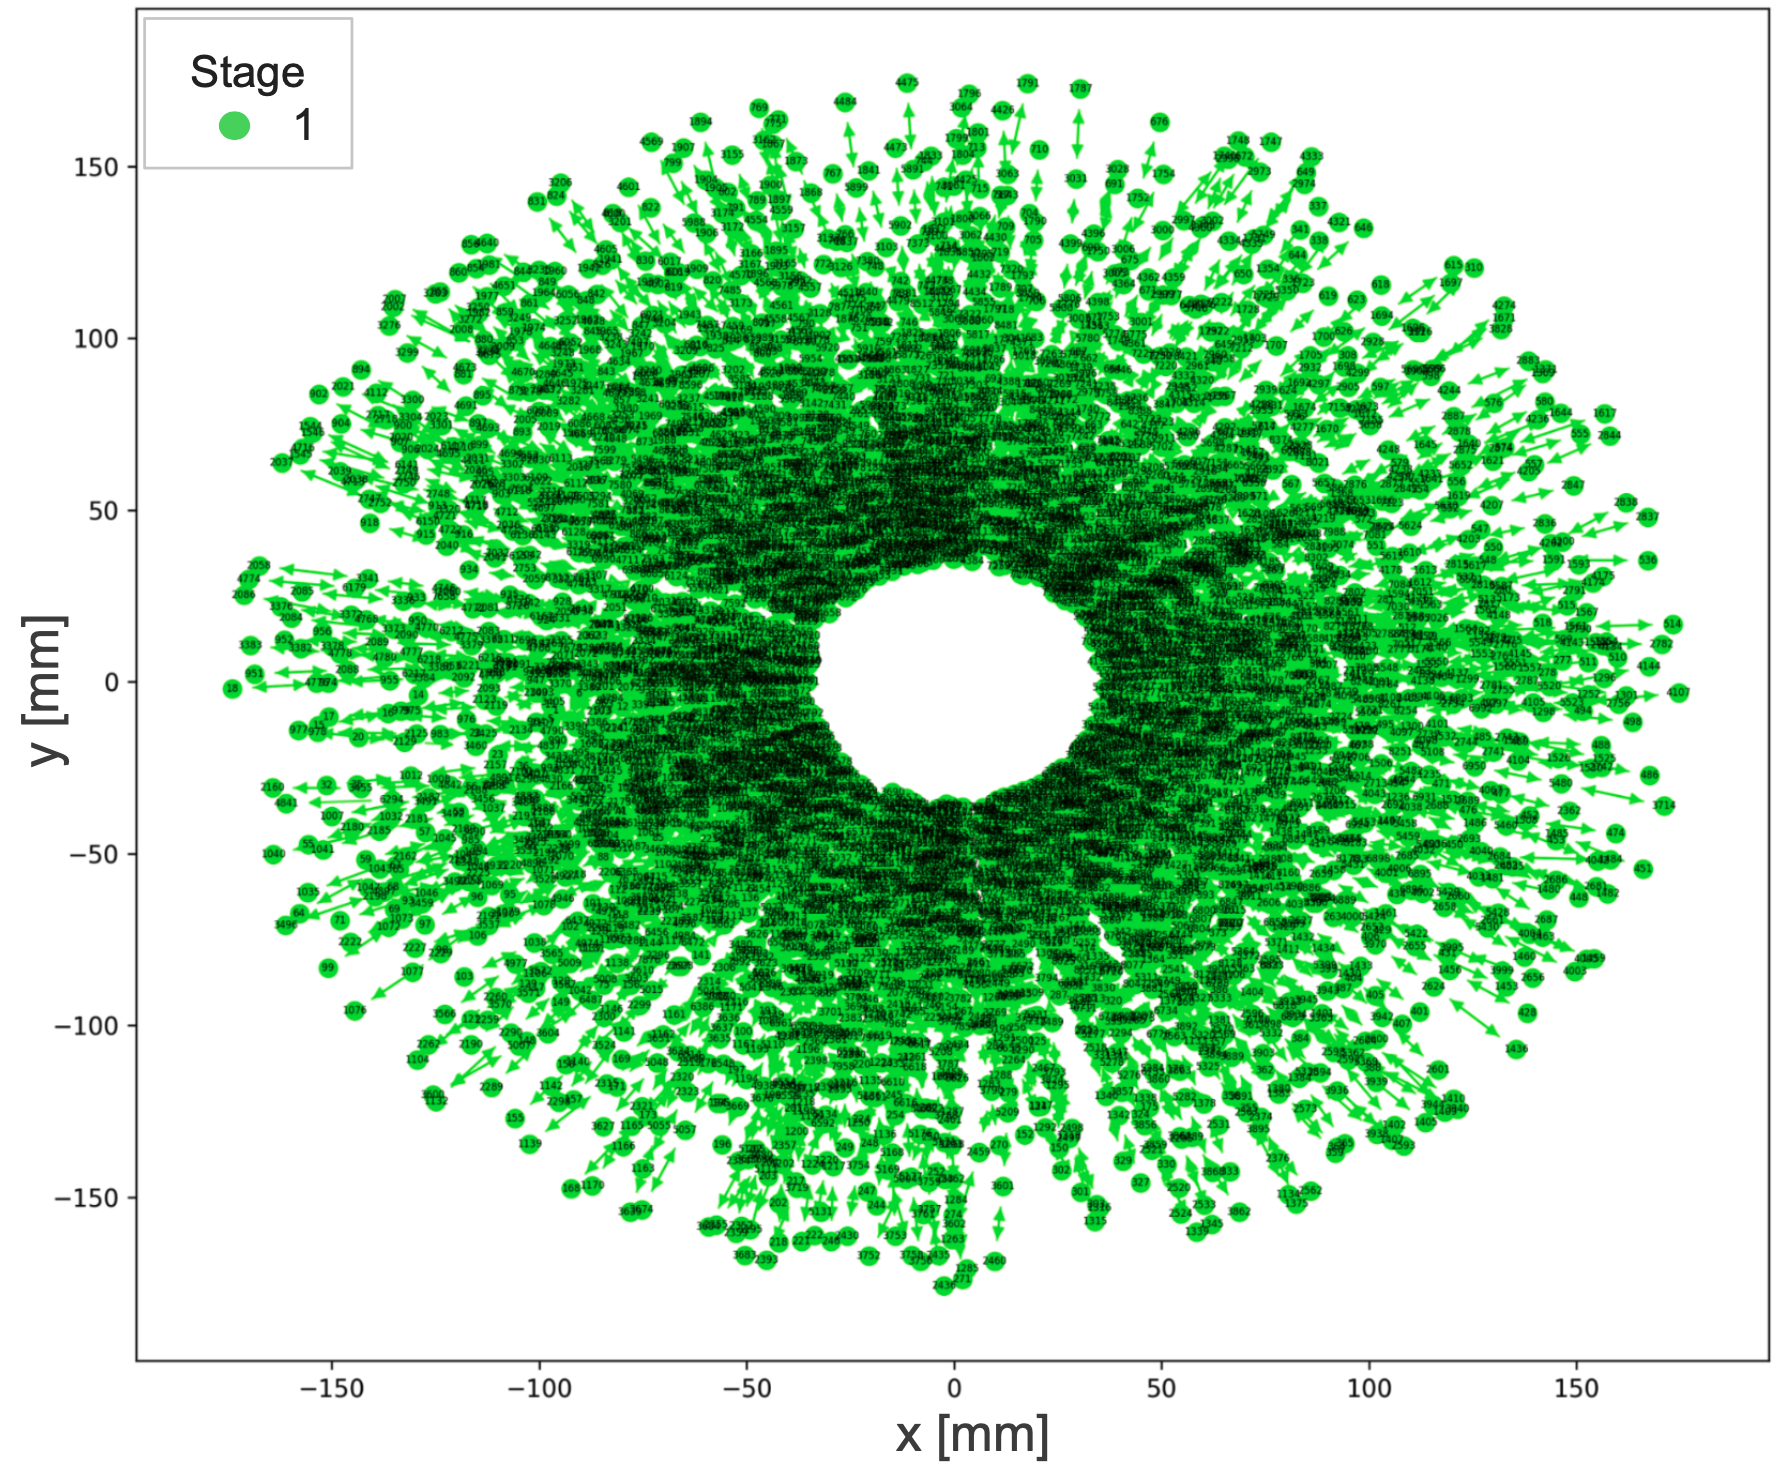
\includegraphics[width=13.5cm]{images/7-results/trackml-endcap-extracted-xy-2.png} } \label{fig:endcap-trackml-extracted-xy}}%
    \hfill
    %\qquad
    \subfloat[]{{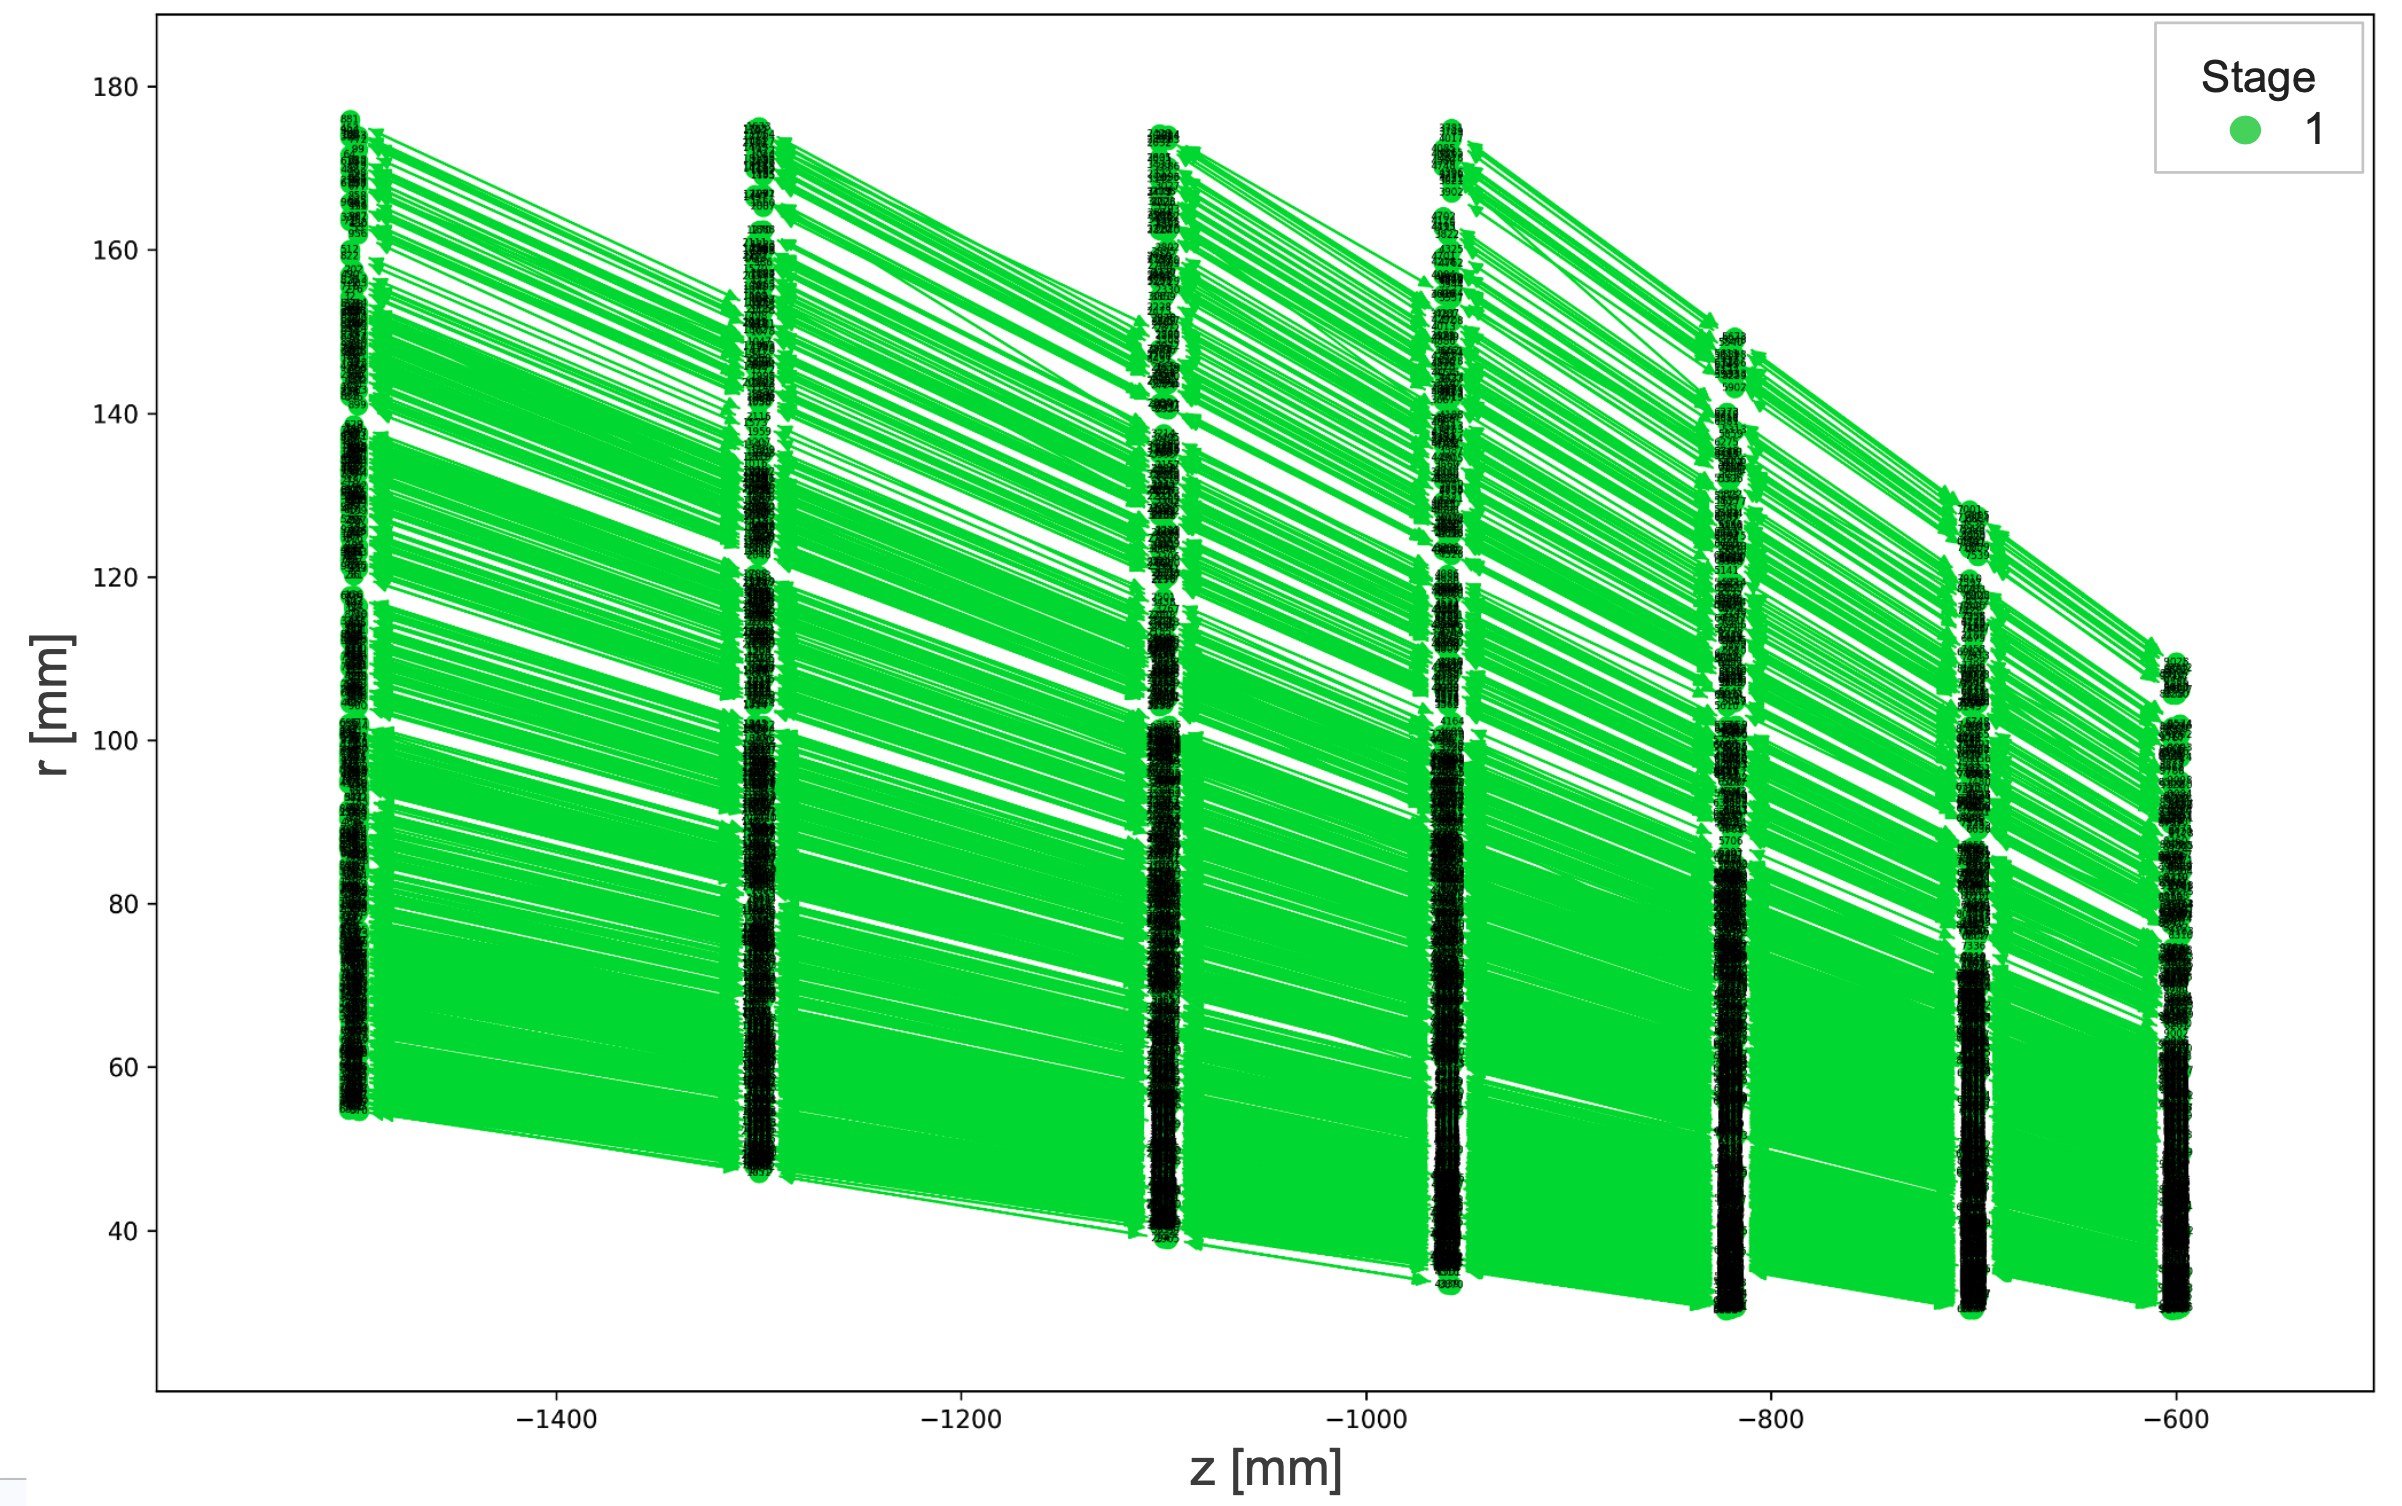
\includegraphics[width=15.5cm]{images/7-results/trackml-endcap-extracted-rz-2.png} } \label{fig:endcap-trackml-extracted-rz}}%
    \caption{Extracted track candidates post Stage 1 of the GNN algorithm applied to the left Pixel endcap (volume 7) of a simulated TrackML detector event, shown from the view of the a) $x$-$y$ plane and b) $r$-$z$ plane. The total number of extracted track candidates post Stage 1 was 1054.}%
    \label{fig:trackml-results-endcap-extracted}%
\end{figure}

\begin{figure}[htbp]%
    \centering
    \subfloat[]{{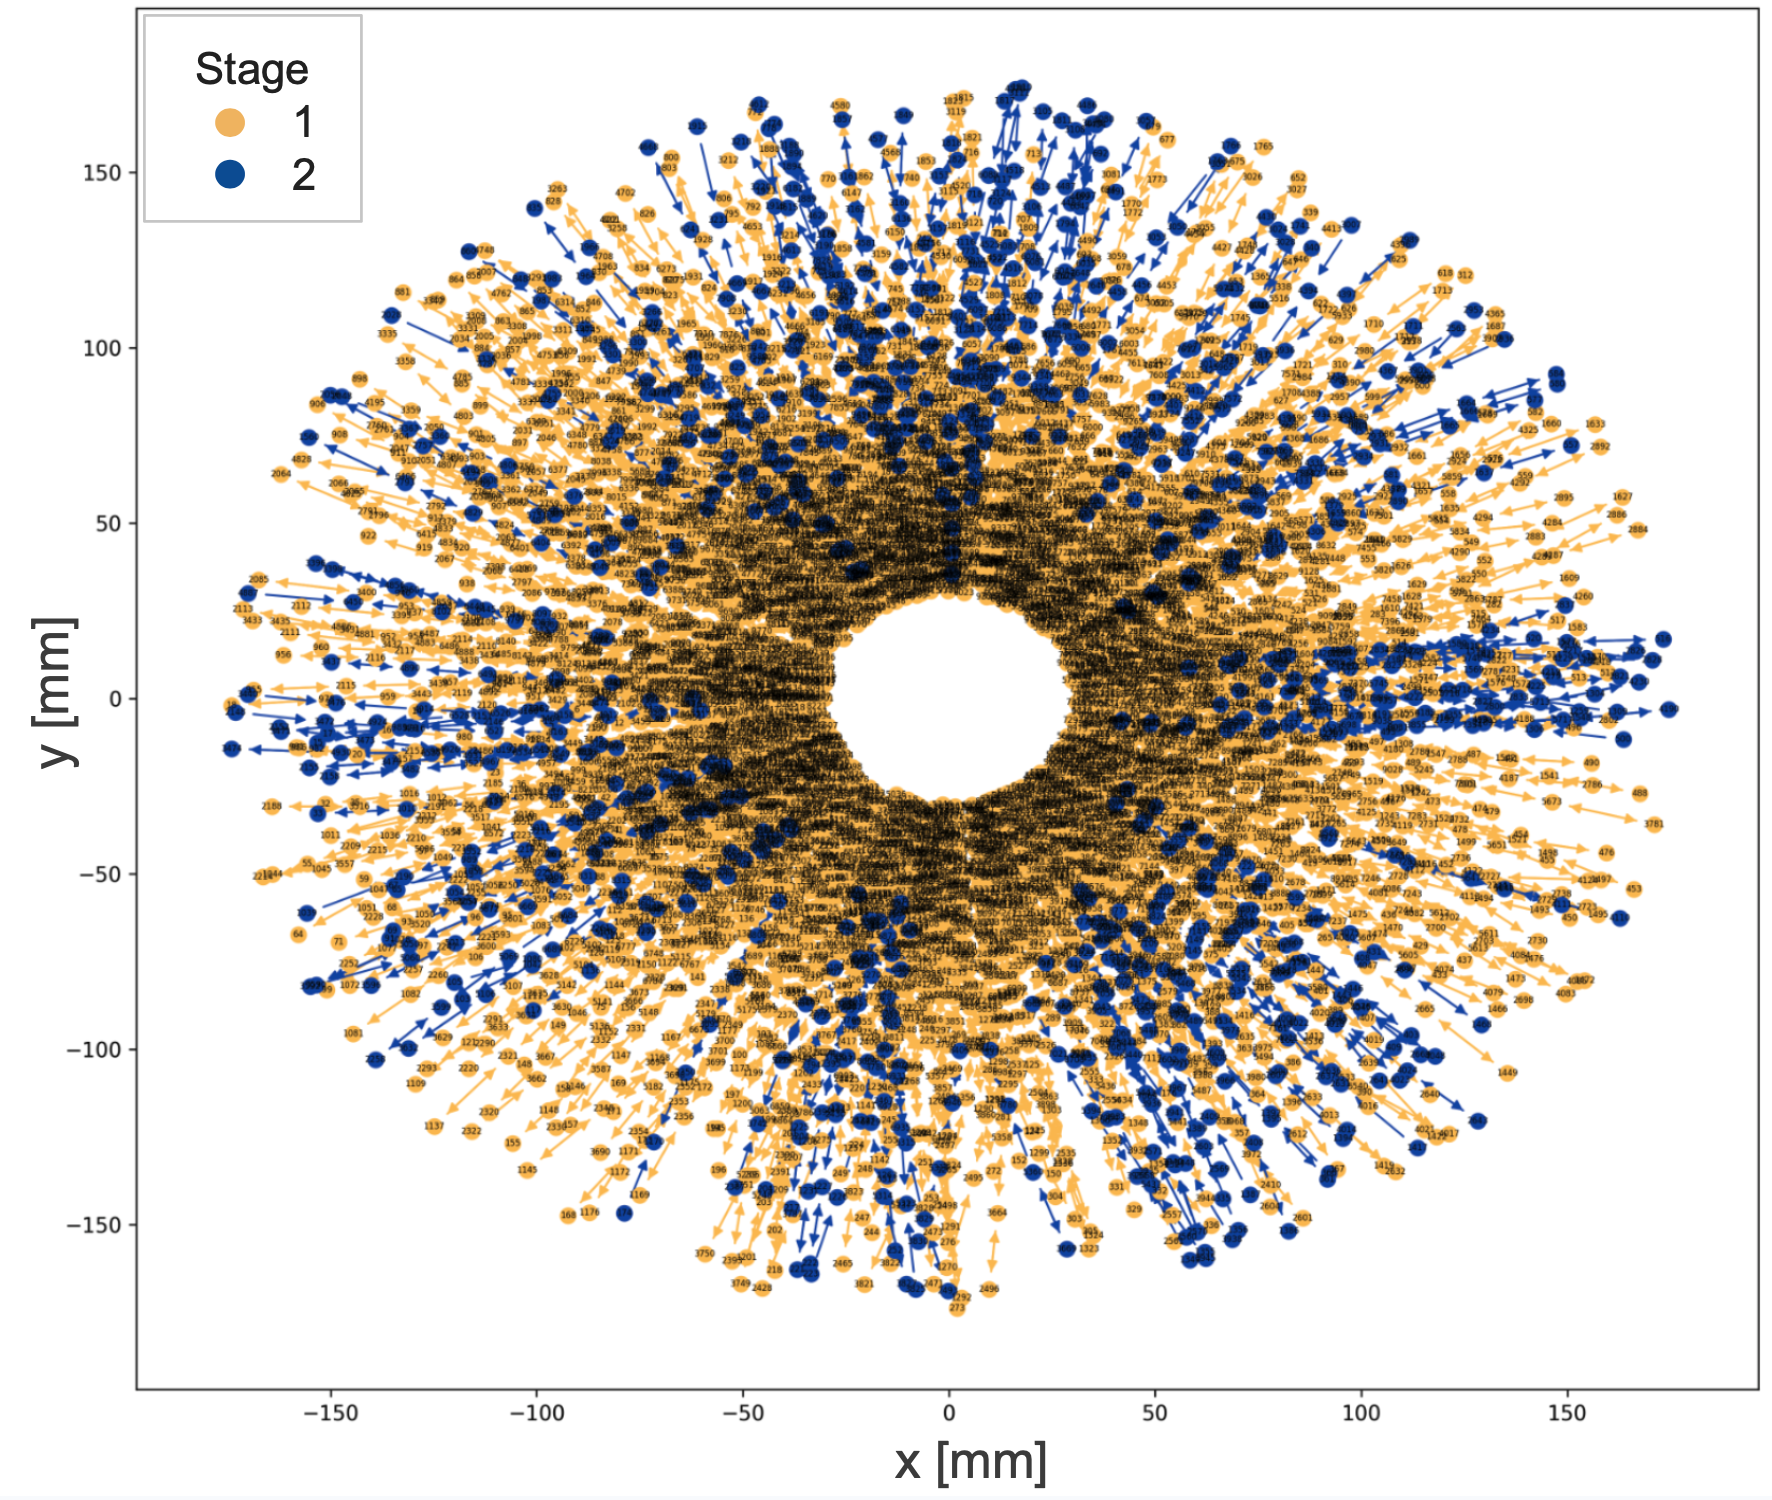
\includegraphics[width=13.0cm]{images/7-results/trackml-endcap-extracted-xy-v2-2.png} } \label{fig:endcap-trackml-extracted-xy-v2}}%
    \hfill
    %\qquad
    \subfloat[]{{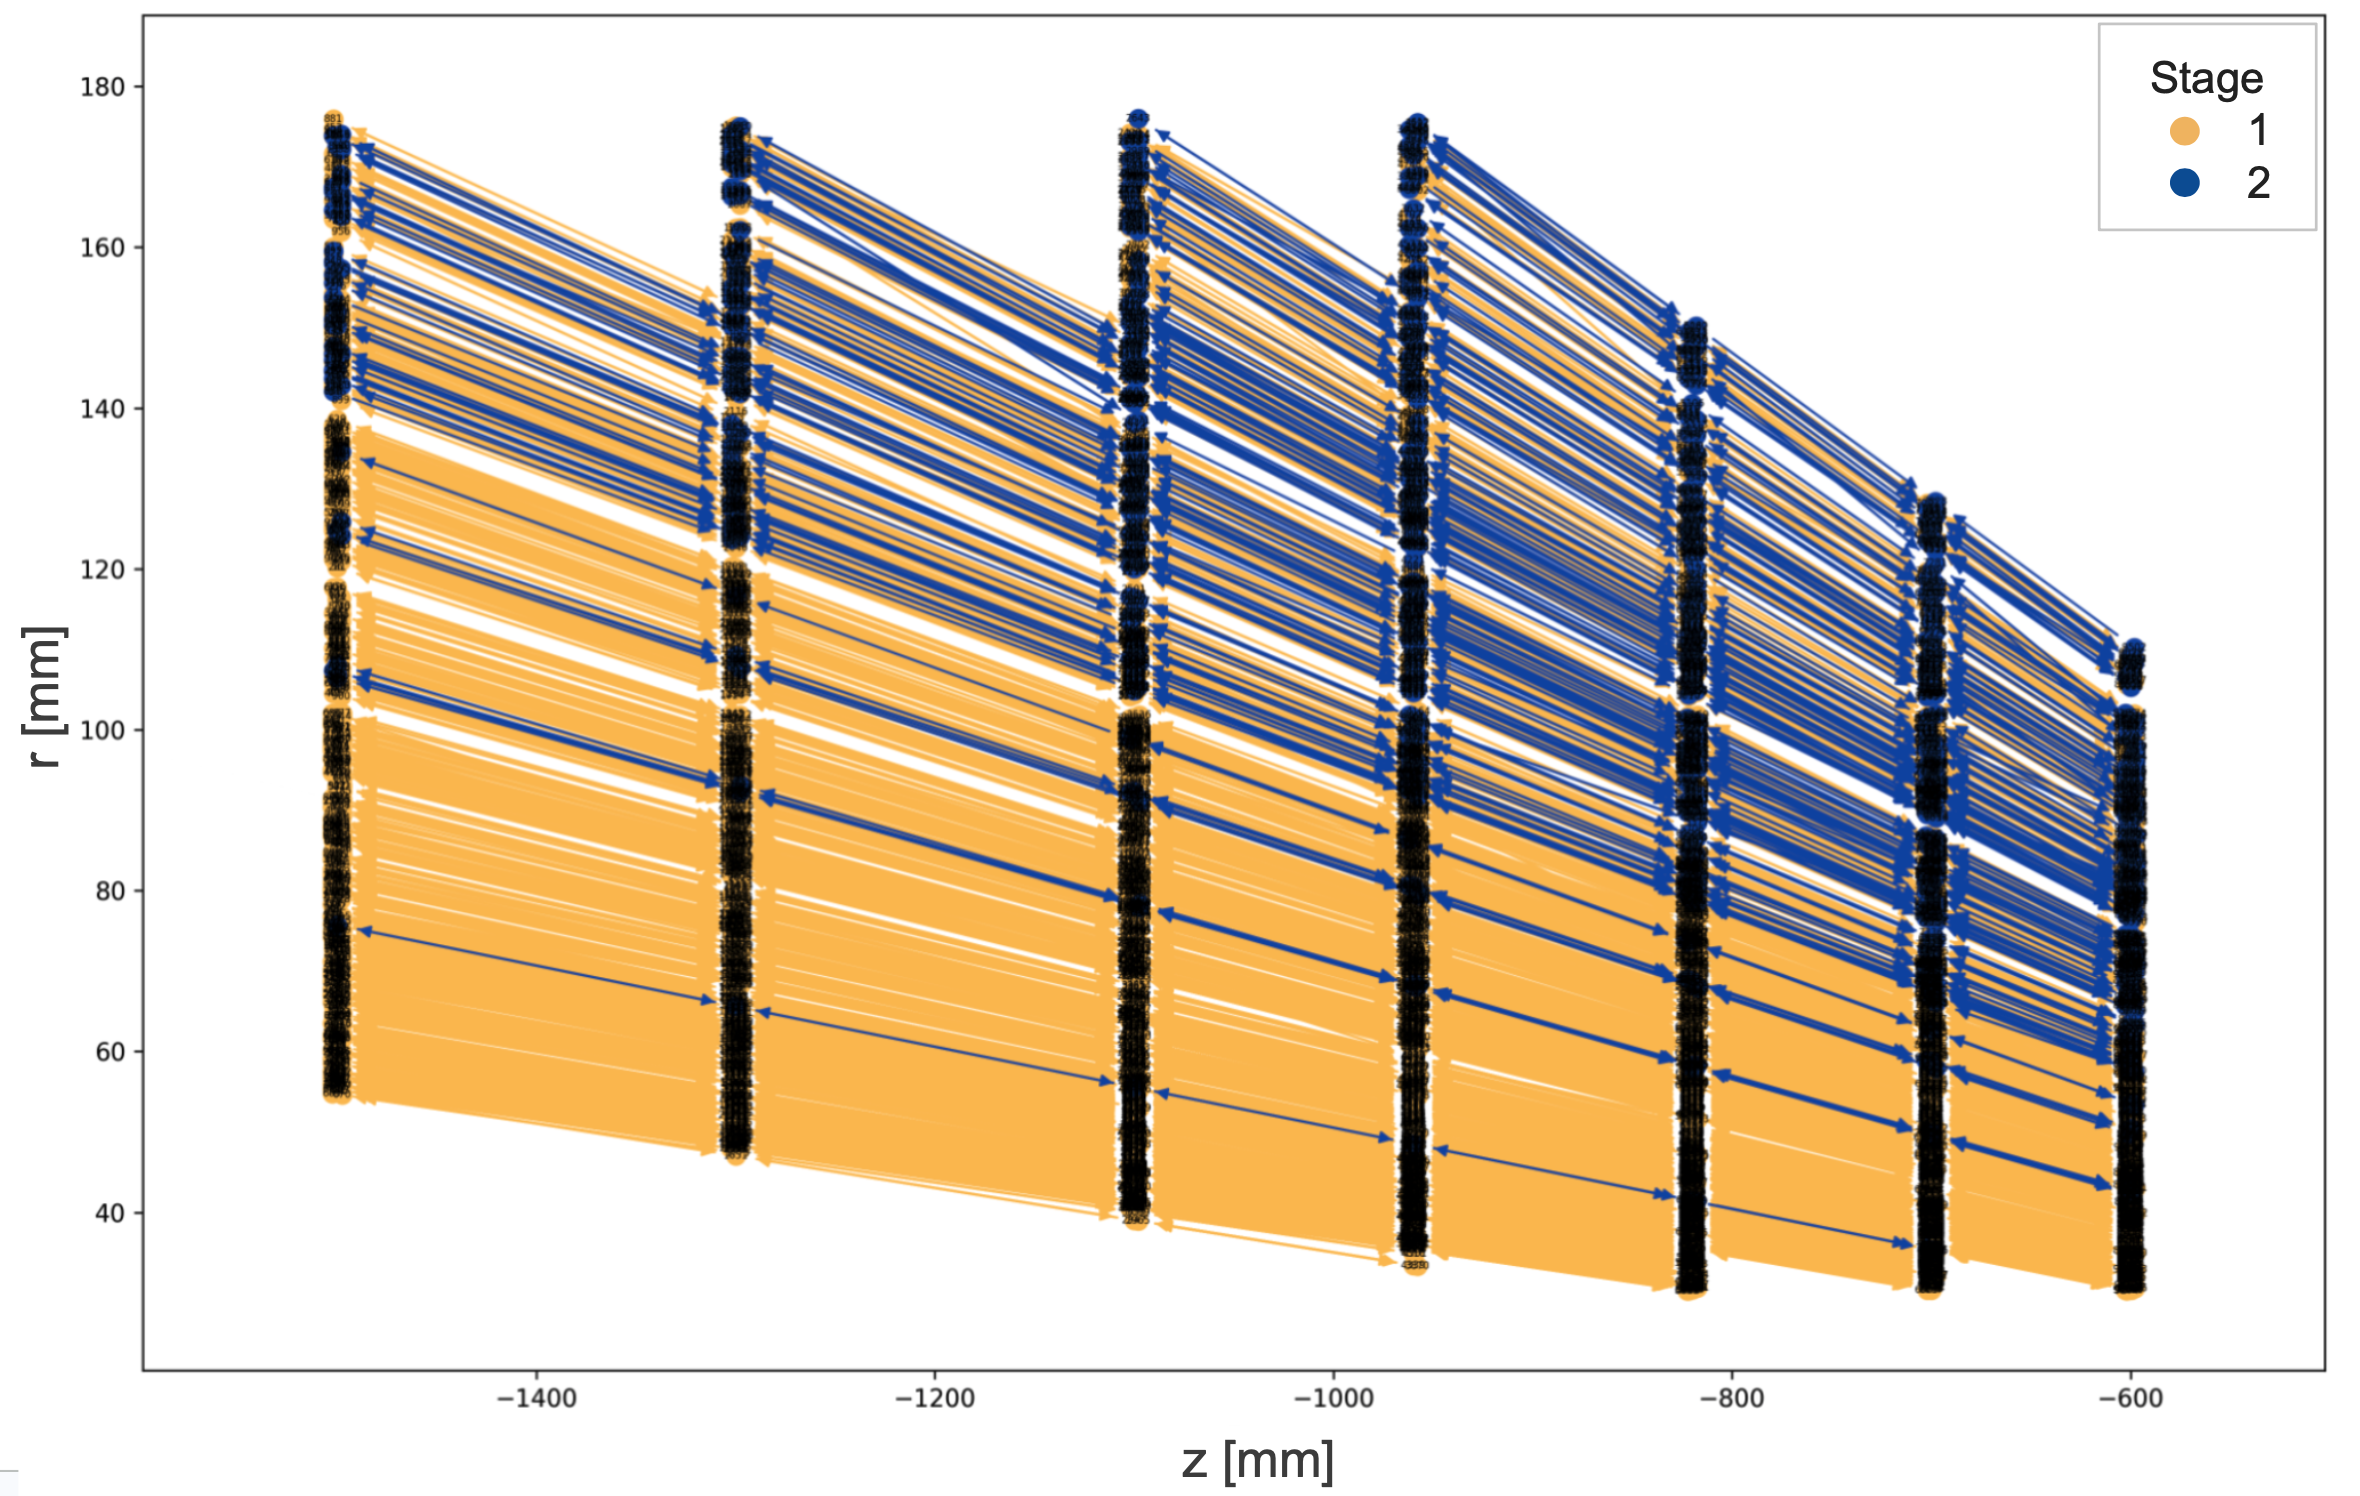
\includegraphics[width=15.0cm]{images/7-results/trackml-endcap-extracted-rz-v2-2.png} } \label{fig:endcap-trackml-extracted-rz-v3}}%
    \caption{Extracted track candidates post Stage 1 and 2 of the GNN algorithm applied to the left Pixel endcap (volume 7) of a simulated event of the TrackML detector model, shown from the view of the a) $x$-$y$ plane and b) $r$-$z$ plane. The total number of extracted track candidates post Stage 1 (orange) was 1054 and post Stage 2 was 265 (blue).}%
    \label{fig:trackml-results-endcap-extracted-v2}%
\end{figure}

It is visible from Figures \ref{fig:endcap-trackml-extracted-xy} and \ref{fig:endcap-trackml-extracted-xy-v2} that track candidates are extracted uniformly within the endcap across all $ 0^{\circ} \leq \phi \leq 360^{\circ}$ during Stage 1 of the GNN algorithm. This is as expected due to the rotational symmetry of the detector in the transverse plane. During Stage 2, we observe the majority of track candidates which are extracted are located at a larger $\theta$ to the $z$-axis (smaller $\eta$). This may be an indication of regions of greater node and edge density, and hence there is a greater proportion of ambiguities to resolve.

The proportion of nodes removed from the main graph network during Stage 1 and Stage 2 were 68\% and 14\% respectively, leaving 18\% of nodes to be further processed. On application of Stage 3 of the GNN algorithm (a further GMR), no additional track candidates were extracted.

% beginning: 9835 nodes
% post stage 1: 3165 nodes
% post stsge 2: 2123 nodes

\subsection{Confusion Matrices}
\label{confusion-matrices-endcap-trackml}

An \textit{outlier edge} is defined to be an edge where its nodes do not belong to the same truth track (truth 1). A \textit{good edge} is defined to be an edge where its nodes do belong to the same truth track (truth 0). The following confusion matrices depict the prediction summary of the GNN algorithm onto the TrackML simulated event, where predicted class 1 indicates the prediction of outlier edges with respect to MC truth and predicted class 0 indicates the prediction of good edges to remain active in the network. The confusion matrix for Stage 1 of the GNN algorithm applied to volume 7 is shown in Figure \ref{fig:confusion-matrix-endcap-stage-1}.


The TPR (and recall) for identification of correct outlier edges achieved was 90.1\%, and the True Negative Rate (TNR) in identification of good edges achieved was 90.5\%. With respect to MC ground truth, the proportion of correct outlier edges identified during Stage 1 of the GNN algorithm, and hence the precision, was found to be 85.1\%. This indicates that the GMR technique of the GNN-algorithm works well for resolving ambiguities in the graph network. The confusion matrix for Stage 2 of the GNN algorithm applied to volume 7 is shown in Figure \ref{fig:confusion-matrix-endcap-stage-2}.

\begin{figure}[htbp]
    \centering
    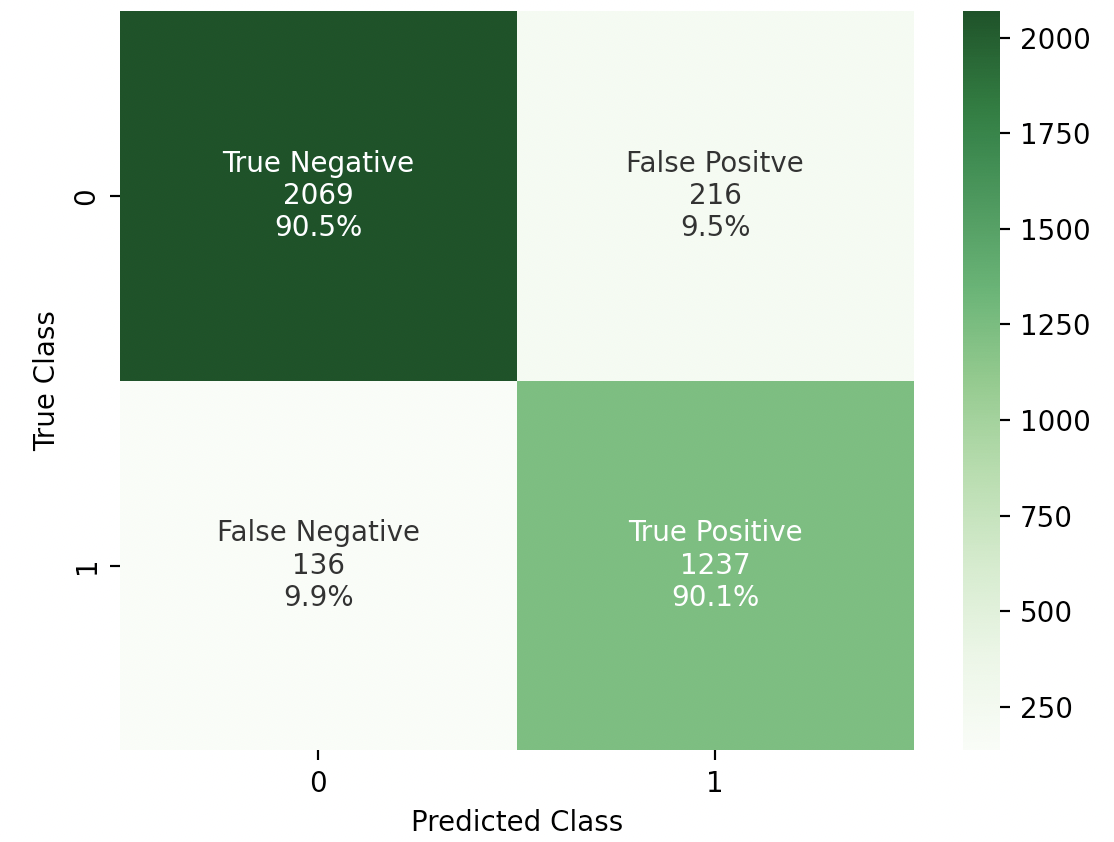
\includegraphics[width=0.78\textwidth]{images/7-results/confusion_matrix_endcap_stage_1.png}
    \caption{Confusion matrix for Stage 1 of the GNN algorithm applied to the Pixel endcap (volume 7) of the TrackML detector model.}
    \label{fig:confusion-matrix-endcap-stage-1}%
\end{figure}
  

\begin{figure}[htbp]
    \centering
    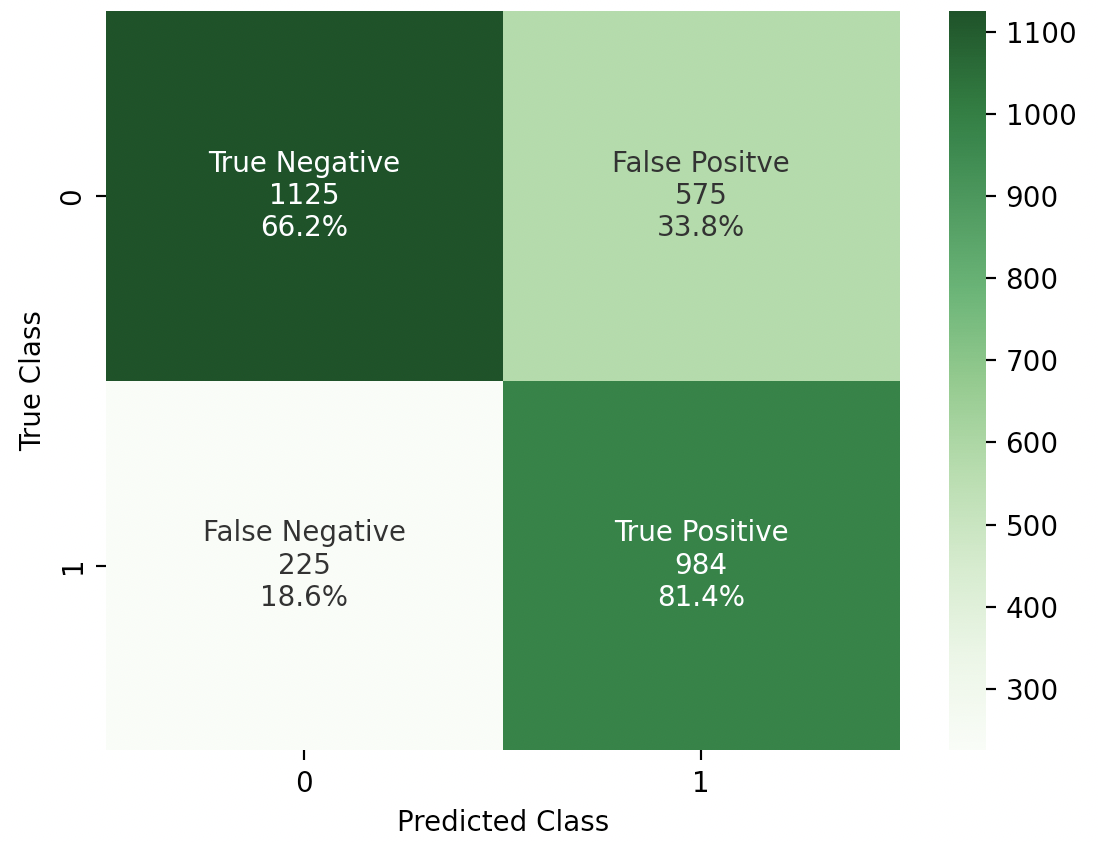
\includegraphics[width=0.78\textwidth]{images/7-results/confusion_matrix_endcap_stage_2.png}
    \caption{Confusion matrix for Stage 2 of the GNN algorithm applied to the Pixel endcap (volume 7) of the TrackML detector model.}
    \label{fig:confusion-matrix-endcap-stage-2}%
\end{figure}


For Stage 2, the TPR for identification of correct outlier edges, and hence the recall, achieved was 81.4\%, and the TNR in identification of good edges achieved was 66.2\%. With respect to MC ground truth, the precision in correct outlier edges identified during Stage 2 was found to be 63.2\%. In comparison to the prediction summary for Stage 1 shown in Figure \ref{fig:confusion-matrix-endcap-stage-1}, the second stage of the GNN algorithm does not discriminate between both classes as well as Stage 1. During Stage 2, we observe an increase in the prediction of false positives. This indicates that the algorithm begins to falsely predict a greater proportion of outlier edges, which will then affect the network connections in further algorithm stages.






\subsection{Track Reconstruction Efficiency and Purity Metrics}

The track reconstruction efficiency, $\epsilon$, provides an indication of the performance of the algorithm and is defined as the ratio of successfully reconstructed reference tracks, to the total number of reconstructable reference tracks in a given volume of interest and is defined by Eq \eqref{eqn:reoncstruction-eff}. 

\begin{equation}
    \epsilon = \frac{n_R}{N_R}
    \label{eqn:reoncstruction-eff}
\end{equation}

where $N_R$ is the number of reconstructable reference tracks and $n_R$ the number of successfully reconstructed reference tracks. Track reconstruction efficiency is calculated by first dissociating graph nodes back to hits, which means that a track candidate is now a collection of hits from several truth particles. A reconstructable reference track is defined as a fully contained track within the volume of interest. As the TrackML detector can produce up to four hits per detector layer, we define a fully contained track to have at least twelve hits within the region of interest. Particles with twelve or more hits and proposed tracks with twelve or more hits are considered. Successfully reconstructed reference tracks are defined as having at least 50\% of its hits from the same truth particle, $N_{hits}$. If $N_{hits} \geq 0.5 \times N_{ref}$, where $N_{ref}$ is the number of reference hits in the volume of interest, then the truth particle reference track is considered as reconstructed. This definition coincides with the definition of reconstruction efficiency stated in the TrackML competition \cite{kaggle-trackml}.

Initially, all reference tracks with $p_{\text{T}} \ge$ 150 MeV are selected and the efficiency is calculated for this. The cut is then increased to select reference tracks with $p_{\text{T}} \ge$ 1 GeV. Table \ref{tab:trackml-track-recon-effs} summarises the track reconstruction efficiencies obtained for fully contained MC truth tracks within volume 7 of the TrackML Pixel detector.


\begin{table}[htbp]
\caption{Summary of track reconstruction efficiencies obtained for fully contained MC truth tracks within volume 7 of the TrackML Pixel detector, which have been extracted using the GNN iterative algorithm developed. $n_R$ is the number of successfully reconstructed reference tracks, $N_R$ is the total number of reconstructable reference tracks and $\epsilon$ is the track reconstruction efficiency. }

\begin{center}
\begin{tabular}{cccc}
\toprule
Threshold & $n_R$ & $N_R$ & $\epsilon$ \\
\hline
$p_{\text{T}} \ge$ 150 MeV    & 1167  & 1347  &  86.6\%    \\
$p_{\text{T}} \ge$ 1 GeV      & 180   & 192   &  93.8\%    \\
\bottomrule
\end{tabular}
\end{center}
\label{tab:trackml-track-recon-effs}
\end{table}

%For fully contained MC truth tracks within volume 7 of the TrackML Pixel detector with $p_{\text{T}} \geq$ 150MeV, the track reconstruction efficiency obtained was 86.2\%, where $n_R = 614$ and $N_R = 712$. Similarly, for fully contained MC truth tracks within volume 7 of the TrackML Pixel detector with $p_{\text{T}} \geq$ 1GeV the track reconstruction efficiency obtained was 93.8\%, where $n_R = 180$ and $N_R = 192$.

% correct data - checked
% pt cut of 150 MeV
% Total num of reconstructed tracks: 1167
% Total num of reference tracks: 1347
% Track reconstruction efficiency:  86.637 %

% pt cut of 1 GeV
% Total num of reconstructed tracks: 180
% Total num of reference tracks: 192
% Track reconstruction efficiency:  93.750 %


Each track is matched with the ground truth majority particle sharing with it the greatest hit number, $N_{truth}$. The ratio of $N_{truth}$ to the number of hits for the reconstructed track, $N_{hits}$, defines the track purity, whilst the ratio of $N_{truth}$ to the number of hits of the underlying particle, $N_{phits}$, defines the particle purity. Both the track purity and particle purity must be greater than 50\%. This criteria coincides with the definition of an accepted track candidate stated in the TrackML competition \cite{kaggle-trackml}.

The purity distributions are shown in Figure \ref{fig:trackml-results-endcap-purity}. The average track purity and particle purity achieved for all extracted candidates in volume 7 after application of the GNN algorithm was 99.0\% for both quantities. There is a small tail in the distribution, however this is negligible as it is several orders of magnitude lower than the main peak. Both purity distributions indicate that the application of the OU process within the KF for track extraction works well to model the influence of the magnetic field for the given $p_{\text{T}}$ range.

\begin{figure}[htbp]
    \centering
    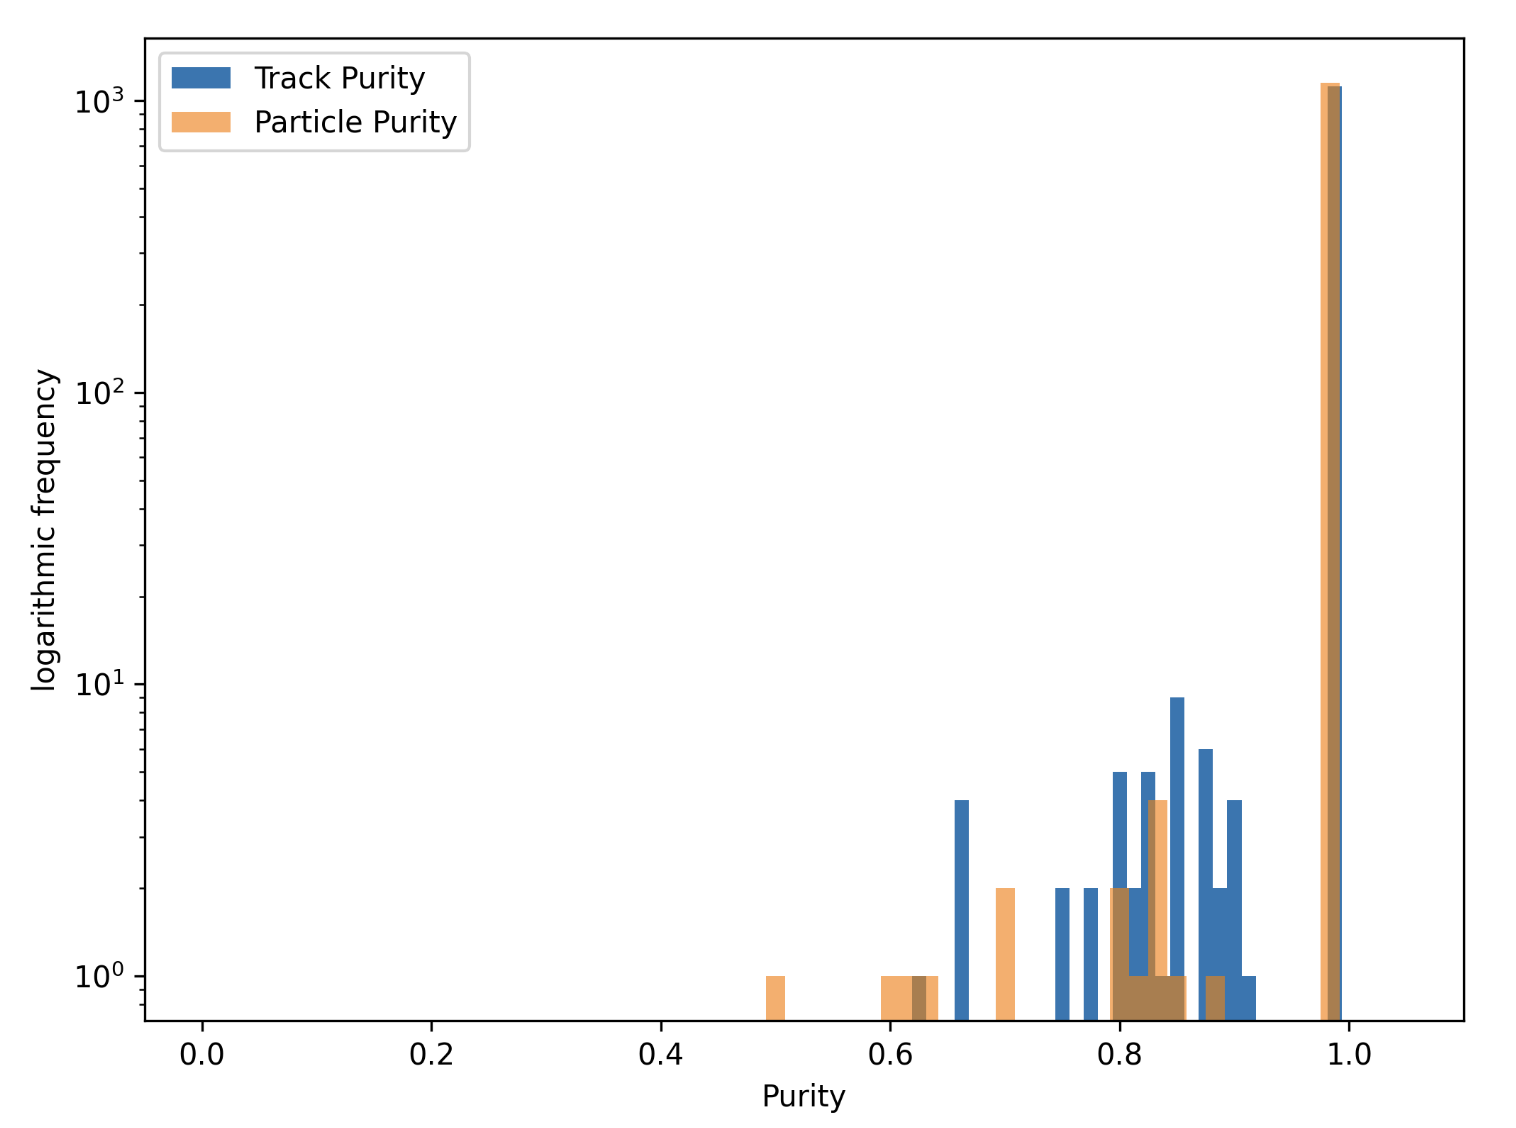
\includegraphics[width=0.75\textwidth]{images/7-results/endcap-purity-log.png}
    \caption{Purity distributions for extracted track candidates after application of the GNN algorithm for track reconstruction within volume 7 of the TrackML Pixel detector with $p_{\text{T}} \geq$ 150MeV.}
    \label{fig:trackml-results-endcap-purity}%
\end{figure}


%present the average over many events here
Executing the GNN algorithm on 50 simulated TrackML events, the average track reconstruction efficiency achieved for fully contained tracks within volume 7 and with $p_{\text{T}} \geq$ 1GeV was 93.3\%. The average track purity and average particle purity achieved were 99.0\% for both quantities.



%\subsection{Performance Evaluation on Volumes 7 and 9}





\subsection{Execution Times}

The GNN algorithm was executed on a MacOS machine, M1 Pro chip, 16GB RAM, with no multi-threaded functions. The average minimum execution time for the GNN algorithm to process 1 event in volume 7 of the TrackML detector, across a total of 50 simulated events, was 45.6s. Table \ref{tab:trackml-endcap-execution-times} and Figure \ref{fig:execution-time-endcap-1} show the breakdown of execution time for each stage of the GNN algorithm. The initialization of the graph network takes up the majority of the execution time, while the remaining algorithmic components comprise 15.9s in execution time. Graph network initialization comprises a conversion of TrackML hit data to nodes and edges, as well as construction of track state estimates $X_{ij}$ and covariances $C_{ij}$. Reading and writing into the graph network implemented using the NetworkX library contributes a significant proportion of execution time, whereas the execution time for each stage of the GNN algorithm, as well as track extraction, is notably small.

\begin{table}[!htbp]
\caption{Breakdown of execution time and cumulative execution time for each stage of the GNN algorithm applied to volume 7 of the TrackML detector.}
\begin{center}
\begin{tabular}{lccc}
\toprule
GNN Algorithm Stage & Time (s) & Cumulative Time (s) & \% \\
\hline
Graph Network Initialization    & 29.7  & 29.7  &  65.1    \\
Stage 1: GMR                    & 3.5   & 33.2   &  7.7    \\
Track Extraction 1              & 4.8   & 38.0   &  10.5    \\
Stage 2: Information Aggregation & 3.2   & 41.2   &  7.0    \\
Track Extraction 2              & 4.4   & 45.6   &  9.6    \\
\bottomrule
\end{tabular}
\end{center}
\label{tab:trackml-endcap-execution-times}
\end{table}

\begin{figure}[htbp]
    \centering
    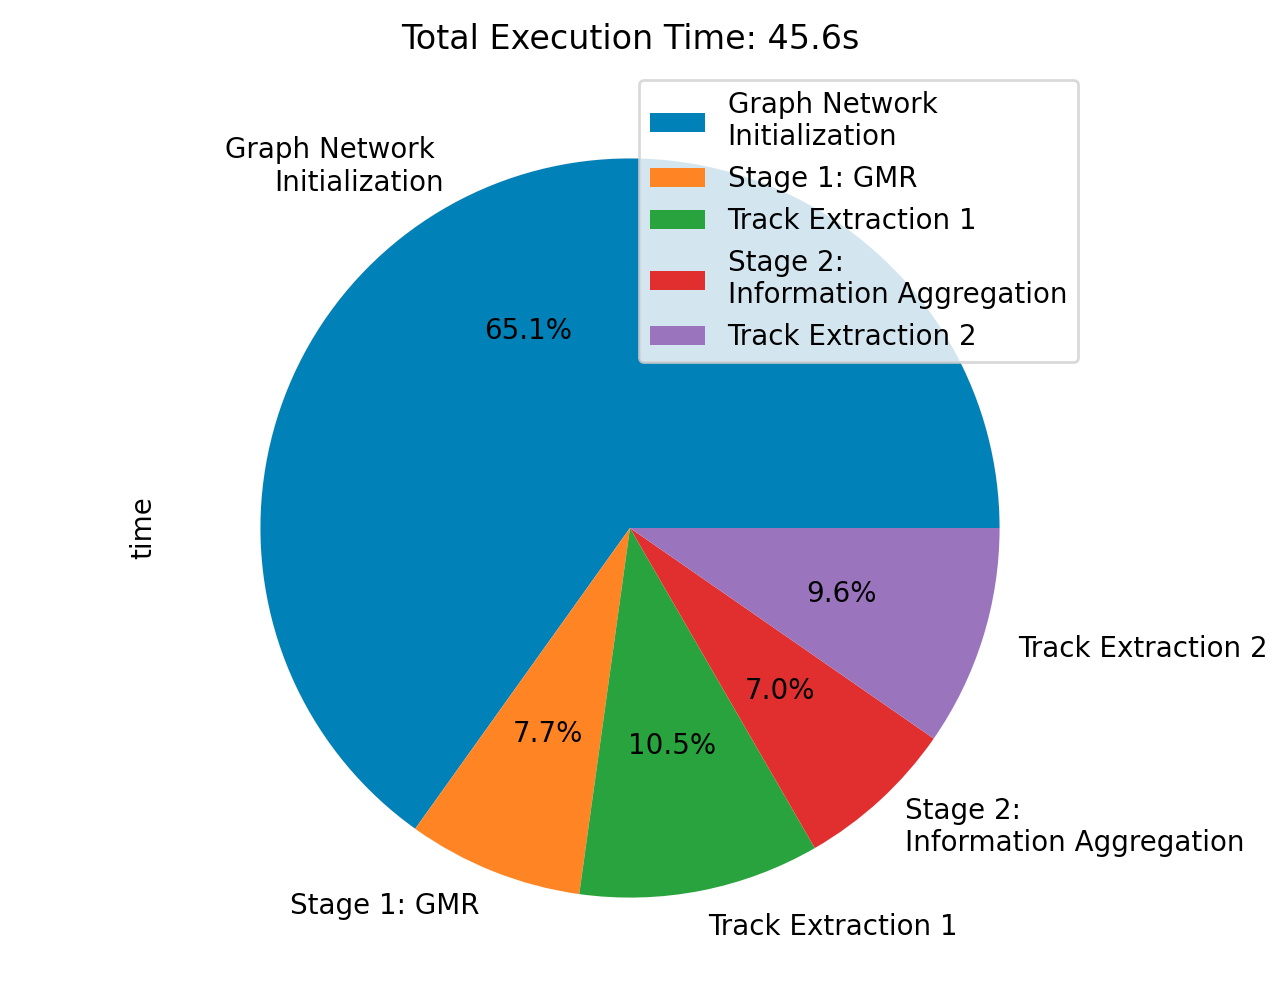
\includegraphics[width=0.7\textwidth]{images/7-results/execution-time-endcap-1.png}
    \caption{Pie-chart of execution time for each stage of the GNN algorithm applied to volume 7 of the TrackML detector.}
    \label{fig:execution-time-endcap-1}%
\end{figure}






%\subsection{Advantages of the KF Implementation}

%An important feature of the KF application is that reconstruction of curved tracks is possible using a low-dimensionality model. By assuming a slow change in track direction, a dynamic model for the KF is constructed using the OU process. The OU process implicitly takes into account the track curvature, without the need to extend the track state to contain additional parameters.


\subsection{Comparison with a Deep Learning Approach}

The iterative graph-based method developed in this thesis can be compared to the graph-based method used by the Exa.TrkX group \cite{Caillou:2815578}. Their approach employs deep geometric learning of track patterns using MLPs and GNNs, as well as a graph segmentation process to identify tracks. The GNN model has an encode-process-decode architecture. The encoder is implemented using two MLPs; one for node features and one for edge features, encoding features into a D-dimensional latent space. At the decode stage, another MLP transforms the latent features of each edge into an edge classification score, representing the probability that the edge portrays two successive space points of a track. The last stage of their pipeline is track reconstruction based on the edge classification score and the graph topology. This process uses a “walkthrough” algorithm, tracing each part of the graph network and selecting the most probable edge, thereby segmenting the graph network in order to separate tracks.

A key difference in the implementation of Exa.TrkX’s method with the method presented in this thesis, is that training of MLPs is executed. This process requires vast amounts of computing resources as their models are trained using a GPU farm. Whereas, the model developed in this thesis is executed on a local CPU environment, requiring far less computational resources and saving energy.

An alternative procedure to the “walkthrough” algorithm used in Exa.TrkX’s graph segmentation process, is the direct application of KFs embedded within the GNN algorithm presented in this thesis. The KF is used for multiple purposes, including track extraction throughout the iterations. The addition of the special dynamic model based on the OU process implemented for the KF is advantageous, as it means that no additional parameters are required in the track state and that reconstruction of tracks is possible using a low-dimensionality model.










\section{Extension to the Pixel Barrel Region}
\label{chapter-7-outlook}


The application of the GNN algorithm is extended to the Pixel barrel region and the right endcap of the TrackML detector, in order to cover the entire Pixel detector volumes $\{7, 8, 9\}$, with reference to Figure \ref{fig:trackml-detector-image}. The graph network is constructed using 38,365 nodes contained within these volumes from the same simulated TrackML event used in Section \ref{chapter-7-endcap-results}, and 201,748 predicted edges are formed using the FASTrack algorithm \cite{Dmitry-fasttrack-addtest}. For this particular test the same initial $p_{\text{T}}$ cut as executed in Section \ref{performance-eval-endcap-vol-7-start} was used for graph segment generation: $p_{\text{T}} \ge 150$ MeV. Figure \ref{fig:trackml-results-barrel-endcap} illustrates the extracted track candidates after application of the GNN algorithm. 

It is clear to see from Figure \ref{fig:trackml-results-barrel-endcap-extracted-xy} that track candidates are extracted uniformly across all $ 0^{\circ} \leq \phi \leq 360^{\circ}$ during Stages 1 and 2 of the GNN algorithm. This is as expected due to the rotational symmetry of the detector in the transverse plane. 

Figure \ref{fig:trackml-results-barrel-endcap-extracted-rz} shows the extracted track candidates viewed from the $r$-$z$ plane, where the algorithm works effectively in both the left and right Pixel endcap regions, however the proportion of track candidates extracted in the Pixel barrel is significantly less. During Stage 1, a total of 1979 track candidates were successfully extracted. During Stage 2 a further 424 track candidates were extracted and in Stage 3 a further 7 track candidates were extracted.

In Stage 1, we observe track candidates extracted uniformly in both endcaps. This is primarily due to the parallel geometry of detector layers and telescopic trajectory of the corresponding tracks, hence there are far fewer ambiguities to resolve in comparison to the barrel region. In contrast to this, during Stage 2 we observe the majority of track candidates extracted are located at a larger $\theta$ to the $z$-axis (smaller $\eta$) in comparison to Stage 1. This is the transition region between the barrel and endcap layers. We also observe a small proportion of track candidates extracted which are contained only within the barrel region as shown in the Figure \ref{fig:trackml-results-barrel-endcap-extracted-rz}.


\begin{figure}[htbp]%
    \centering
    \subfloat[]{{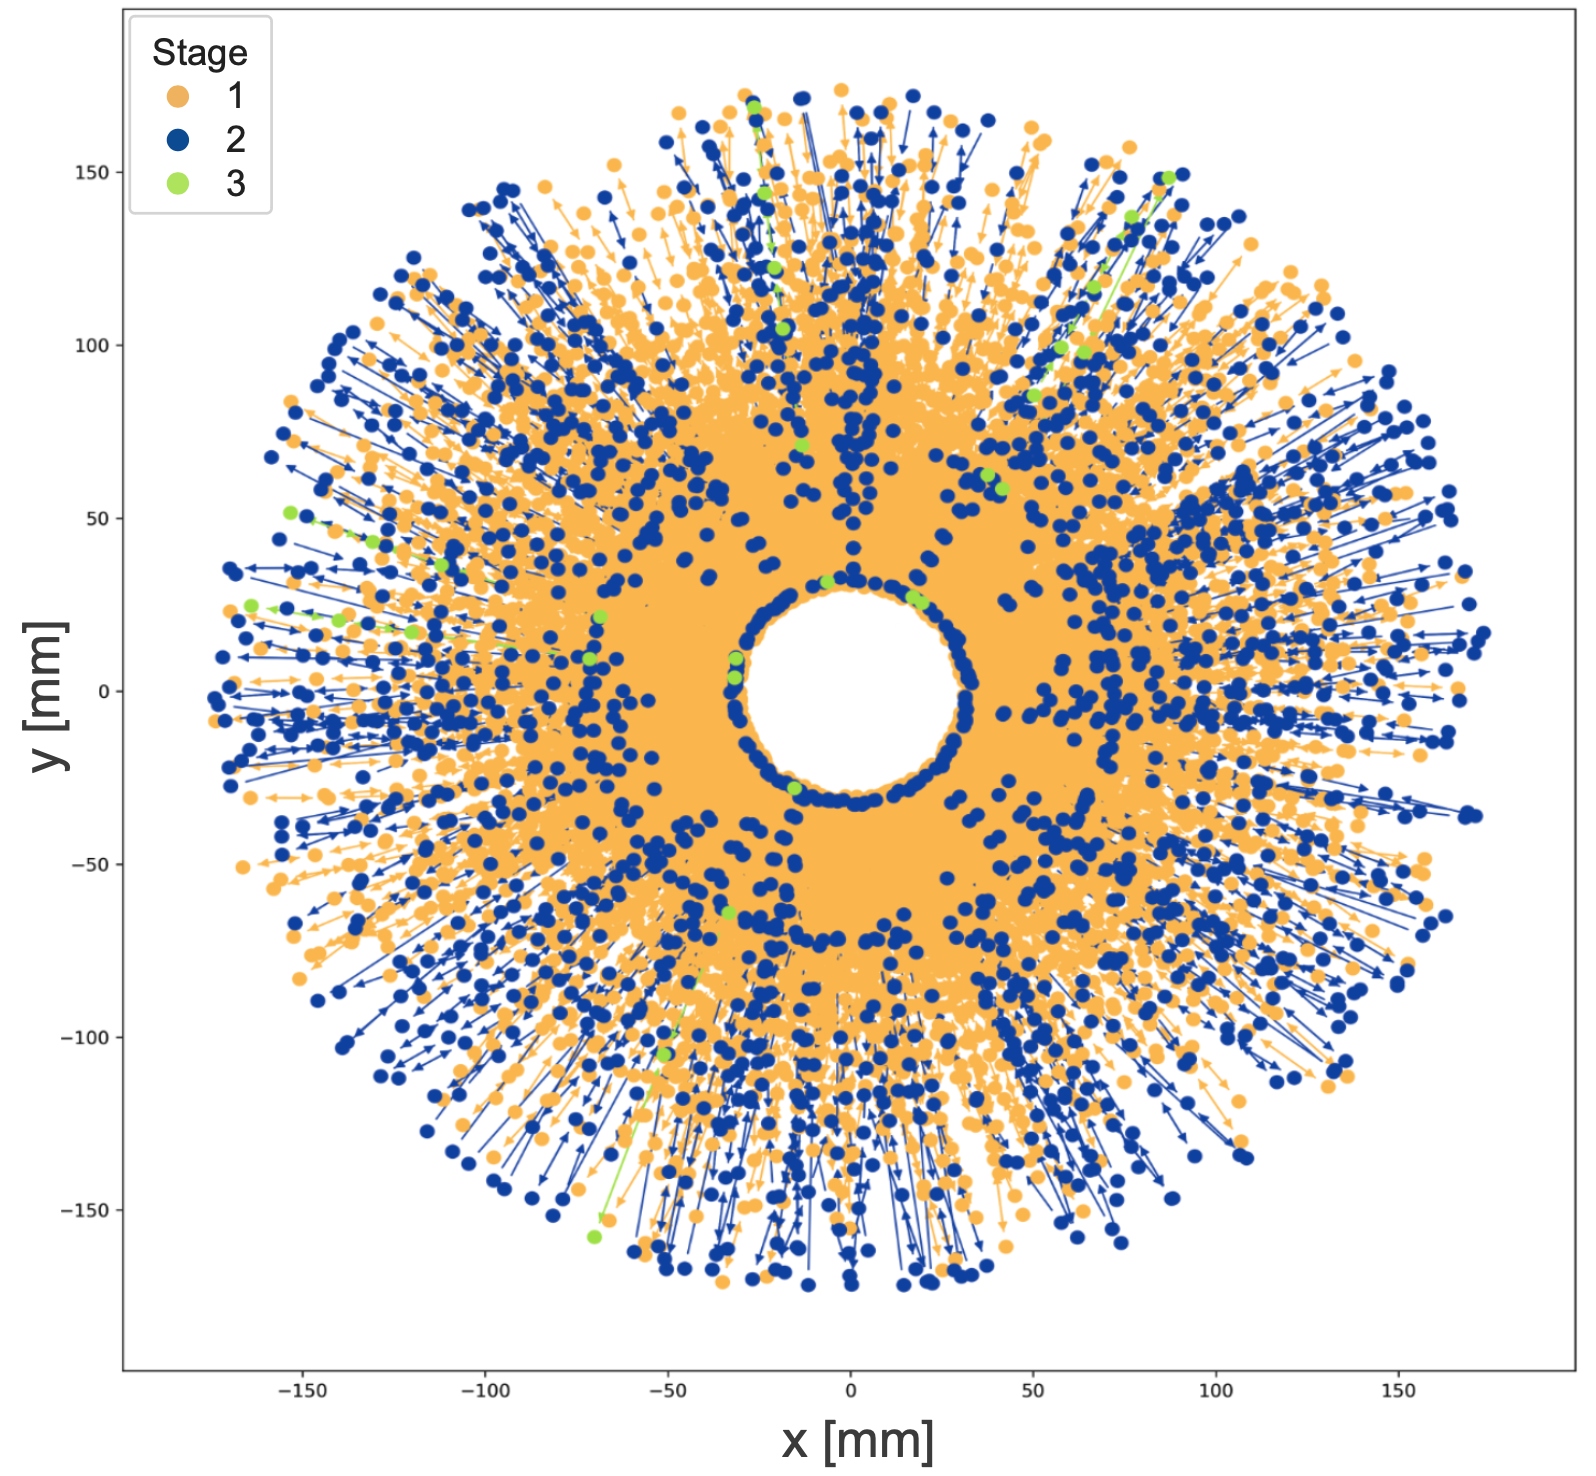
\includegraphics[width=11.5cm]{images/7-results/trackml-endcap-barrel-extracted-xy-v2.png} } \label{fig:trackml-results-barrel-endcap-extracted-xy}}%
    \hfill
    %\qquad
    \centering
    \subfloat[]{{\includegraphics[width=15cm]{images/7-results/trackml-endcap-barrel-extracted-rz-v2.png} } \label{fig:trackml-results-barrel-endcap-extracted-rz}}%
    \caption{Extracted track candidates post application of the iterative GNN algorithm onto the Pixel detector of the TrackML model. Track candidates are iteratively extracted after each stage of the GNN algorithm, shown by the legend. The total number of extracted track candidates at Stage 1 (orange) was 1979, at Stage 2 was 424 (blue) and at Stage 3 (green) was 7.}%
    \label{fig:trackml-results-barrel-endcap}%
\end{figure}






\subsection{Confusion Matrices}

The following confusion matrices depict the prediction summary of the GNN algorithm onto the TrackML simulated event, where predicted class 1 indicates the prediction of outlier edges with respect to MC truth and predicted class 0 indicates the prediction of good edges to remain active in the network. The confusion matrix for Stage 1 of the GNN algorithm applied to the Pixel barrel and endcap regions is shown in Figure \ref{fig:confusion-matrix-barrel-endcap-stage-1}.


The TPR for identification of correct outlier edges achieved was 92.3\%, and the True Negative Rate (TNR) in identification of good edges achieved was 84.9\%. With respect to MC ground truth, the proportion of correct outlier edges identified during Stage 1 of the GNN algorithm, and hence the precision, was found to be 95.6\%. The recall in correct outlier edges identified during Stage 1 was 92.3\%. Similar to Section \ref{confusion-matrices-endcap-trackml} these results indicate that the GMR technique of the GNN-algorithm works well for resolving ambiguities in the graph network.

\begin{figure}[htbp]
    \centering
    \includegraphics[width=0.79\textwidth]{images/7-results/confusion_matrix_barrel_stage_1.png}
    \caption{Confusion matrix for Stage 1 of the GNN algorithm applied to the Pixel barrel and endcap of the TrackML detector model.}
    \label{fig:confusion-matrix-barrel-endcap-stage-1}%
\end{figure}

The confusion matrix for Stage 2 of the GNN algorithm applied to the Pixel barrel and endcap regions is shown in Figure \ref{fig:confusion-matrix-barrel-endcap-stage-2}.


\begin{figure}[htbp]
    \centering
    \includegraphics[width=0.79\textwidth]{images/7-results/confusion_matrix_barrel_stage_2.png}
    \caption{Confusion matrix for Stage 2 of the GNN algorithm applied to the Pixel barrel and endcap of the TrackML detector model.}
    \label{fig:confusion-matrix-barrel-endcap-stage-2}%
\end{figure}

For Stage 2, the TPR for identification of correct outlier edges, and hence the recall, achieved was 48.1\%, and the TNR in identification of good edges achieved was 46.1\%. With respect to MC ground truth, the precision in correct outlier edges identified during Stage 2 was found to be 67.5\%. In comparison to the prediction summary for Stage 1 shown in Figure \ref{fig:confusion-matrix-barrel-endcap-stage-1}, the second stage of the GNN algorithm does not discriminate between both classes as well as Stage 1, as there is a much greater proportion of false positives and false negatives. This suggests that the algorithm begins to falsely predict a greater proportion of outlier edges, which will then affect the network connections in further algorithm stages.




%\subsection{Track Reconstruction Efficiency and Purity Metrics}


% \begin{figure}[htbp]
%     \centering
%     \includegraphics[width=0.7\textwidth]{images/7-results/endcap-purity.png}
%     \caption{Purity distributions for application of the GNN algorithm for track reconstruction on the Pixel barrel and endcap regions of the TrackML detector}
%     \label{fig:trackml-results-endcap-barrel-nodes-purity}%
% \end{figure}


% \subsection{Execution Times}



% \subsection{Remaining Network Post Track Extraction}

% The node density in the barrel is ... times greater compared to the endcap regions, and the edge density is .... which is a contributing factor towards this.

% \begin{figure}[htbp]
%     \centering
%     \includegraphics[width=0.99\textwidth]{images/7-results/trackml-barrel-remaining-node-degree.png}
%     \caption{TODO: regenerate this plot but with the node degree inverted!!! }
%     \label{fig:trackml-results-barrel-endcap-remaining-node-degree}%
% \end{figure}







\section{Improvements and Other Approaches}



\subsection{Improvement for Extrapolation in r-z Plane}

In general, a track state in $r$-$z$ plane is defined as a track position at some reference surface (constant radius $r$ or constant $z$ position) and the inverse track inclination angle as outlined in Eq \ref{eqn:kf-track-fit-initialised-state-rz}. Due to the orientation of the detector layers, the extrapolation can result in a change of reference surface type. One such example is an extrapolation from the Pixel barrel layer at constant $r$ to Pixel endcap layer at constant $z$, as illustrated in Figure \ref{fig:improvement-extrapolation}. Naturally, there are four possible cases for extrapolation; barrel-to-barrel, barrel-to-endcap, endcap-to-barrel and endcap-to-endcap, and each case should be considered individually.


\begin{figure}[htbp]
    \centering
    \includegraphics[width=0.8\textwidth]{images/7-results/improvement-extrapolation.png}
    \caption{Illustration of track state extrapolation from node A located in a barrel layer at constant radius $r$, to the target node, node T located in an endcap layer at constant $z$-position.}
    \label{fig:improvement-extrapolation}%
\end{figure}


The initial track state is at node A with its $z$-position and some estimate of inverse track inclination $\tau_A$. The final track state is at a target node T with its $z$-position and consists of an extrapolated $r$-position and $\tau_T$. This is described by Equations \eqref{eqn:extrapolation-improvement-1}  and \eqref{eqn:extrapolation-improvement-2}, and hence this model would lead to a different form of the extrapolation Jacobian.

\begin{equation}
    \begin{bmatrix} z_A \\ \tau_A \end{bmatrix} 
    \rightarrow
    \begin{bmatrix} r_T \\ \tau_T \end{bmatrix} 
    \label{eqn:extrapolation-improvement-1}
\end{equation}

\begin{equation}
    r_T = r_A + \frac{z_T - z_A}{\tau_A}, \quad \tau_T = \tau_A
    \label{eqn:extrapolation-improvement-2}
\end{equation}


Exploring this general case of extrapolation in the $r$-$z$ plane is one such enhancement for the implementation of the KF and may provide an improvement in the precision of track state estimates.







\subsection{Software Optimisations}

Several computational refinements and software optimisations that can be done in order to improve the implementation of the GNN algorithm are discussed here.

With regards to algorithm implementation, the Python library \textit{Numpy} \cite{harris2020array} is utilised for all matrix computations between track state vectors. This allows for scalability and reduces processing time, specifically for highly dense environments with large numbers of graph nodes. However, in general many other optimisations can be implemented in order to eliminate redundancies in code. These include using the most efficient data structures appropriate to the problem, avoiding unnecessary Input/Output such that the algorithm only reads and writes to files when absolutely necessary, as well as reducing code complexity.

With reference to Figure \ref{fig:execution-time-endcap-1}, from these observations it was found that the greatest execution time was during the graph network initialization stage, specifically during the reading and writing of metadata to the network nodes. An alternative procedure that can be explored here is the use of Numpy arrays for data storage.

Another software optimisation includes the use of GPU implementation. This would allow significant speed up due to its superior processing power and greater memory storage. GPUs can handle many more mathematical calculations at once with greater efficiency compared to CPUs and would be vital for the improvement of the GNN algorithm. One such implementation of this would be using the Python package \textit{CuPy} \cite{cupy_learningsys2017}, to leverage GPU accelerators by replacing all Numpy implementations. All aspects mentioned above are necessary improvements for the algorithm to be considered for proper online usage in track finding software in detector experiments.







\subsection{Community Detection}

If a subgraph does not meet the criteria to qualify as a good track candidate outlined in Section \ref{gnn-track-extration}, a technique known as \textit{Community Detection} \cite{community} is applied in order to further partition the set of nodes. Community Detection is a generalisation of CCA and works by using a distance metric, typically modularity, in order to label nodes into groups such that all nodes in a group are \textit{closely connected}. Modularity is a benefit function that measures the strength of a particular division of a network using the number of edges and edge weights. A popular modularity maximisation approach is the Louvain method \cite{python_louvain}, which iteratively optimises local communities until global modularity can no longer be improved. An example illustration of a network partition via Community Detection using modularity is shown in Figure \ref{fig:community-detection}. 

\begin{figure}[htbp!] 
    \centering
    \subfloat[]{%
        \includegraphics[width=0.45\linewidth]{images/7-results/community-detection-1.png}%
        \label{fig:community-detection-1}%
        }%
    \hfill%
    \subfloat[]{%
        \includegraphics[width=0.45\linewidth]{images/7-results/community-detection-2.png}%
        \label{fig:community-detection-2}%
        }%
    \caption{Example application of the Community Detection algorithm applied to a small group of nodes from a TrackML event. a) Subset of nodes and edges connected as one subgraph shown in red. b) Post application of the Community Detection algorithm. Separation of the subgraph in a) into potential track candidates represented by separate colours. The faint grey edges show connections that have been deactivated through Community Detection.}
    \label{fig:community-detection}
\end{figure}

Figure \ref{fig:community-detection-1} shows a small subset of nodes from a TrackML event and its corresponding edges connected as one subgraph. The general shape of the network gives an indication that the tracks originate from the left-hand side, where the trajectories move towards the right-hand side. The results of application of Community Detection are shown in Figure \ref{fig:community-detection-2}. In this instance, the Community Detection was successful to partition the network into a total of seven subgraphs shown by separate colours. Six of these subgraphs met the criteria for a good track candidate, and a single track fragment was also formed shown by the grey subgraph containing two nodes. However upon further investigation, this procedure did not work successfully in all cases, specifically in dense environments, and the algorithm was found to not utilize node properties during network partition. Therefore, as this procedure needed further refinement, it was not implemented into the main GNN pattern recognition algorithm. 

A technique such as Community Detection is advantageous for a problem such as track splitting, as it provides fast convergence in track extraction, given that the algorithm is adapted for highly dense environments.





\section{Conclusion}

It is promising to see that the GNN algorithm works on simulated particle collision events produced by the TrackML detector, which have significant track multiplicity. The proposed GNN algorithm is successful in identifying outlier edge connections in an iterative manner, as well as successful in extracting track candidates for the endcap regions. It is an encouraging result that this methodology provides a high performance for fully contained tracks within the endcap volume, achieving 93.3\% average track reconstruction efficiency for tracks with $p_{\text{T}} >$ 1GeV averaged over 50 simulated TrackML events. The average track purity and average particle purity achieved were 99.0\% for both quantities. Overall, the application to the endcap region is highly successful.

Neighbourhood complexity is inferred by the network, this is observed as the GNN algorithm automatically initiates the pattern recognition process in regions where outlier connections are easily identifiable. The network starts with low density regions (both endcap regions) and gradually progresses towards higher density areas (the transition between the barrel and endcap layers). This shows that the GNN algorithm behaves as expected.

However the algorithm requires significant refinement and further improvement for application to the Pixel barrel region. A deeper understanding is needed in order to evaluate the behaviour of the network on the Pixel barrel region and assess the quality of its performance. Further work would include improvement of Stage 2 of the GNN algorithm in order to improve the TPR and TNR, as well as analysis of the remaining network within the barrel region.

%------------------------------------
%	7. Summary & Outlook
%------------------------------------


\chapter{Summary and Outlook}
\label{chapter-8}

%\subsection{Current Limitations and Refinements}

%\textbf{TODO Here!!}
%Possibly move this to chapter 8 outlook - further work and discussion, current limitations and refinements. These points have been scattered in the main text, this section is mainly a summary of them to present in a easible readable manner. clustering k=1 scenario, pragmatic choices etc, the density of barrel hits and second set of data, retraining certain thresholds and analysing the performance of the algorithm on the ITk geometry to give an indication ... with more time permitting further research and analysis can be conducted to investigate possible improvements. Other considerations and avenues to explore have been discussed below...






% 1. Intro & background

The current algorithms employed to reconstruct tracks for High-Energy particle detectors have proven to be very powerful. These methods include seeded track following and the combinatorial KF. However, they are not designed to handle the conditions presented by extreme environments such as the HL-LHC, as these approaches do not scale well as the seed number grows. As discussed in Chapter \ref{chapter-2}, the task of track reconstruction becomes increasingly difficult as the luminosity increases. The collision rate and hence hit occupancy will also grow significantly during future upgrades of the LHC program. Therefore, novel and precise tracking methodologies, as well as efficient use of computing power, are paramount for track reconstruction. The heart of the problem tackles the simultaneous consideration of reducing the amount of CPU usage, and hence the environmental impact, as well as maintaining the ability to reconstruct tracks with minimal loss in efficiency. As such, enhancements in track reconstruction algorithms are imperative for the future growth of particle detector experiments. 

The use of ML algorithms for track reconstruction has provided a route to develop methodologies that can save vast amounts of CPU resources. An original approach has been explored in great detail in this thesis utilising GNN architectures for efficient track reconstruction. This process begins with a procedure to construct a graph network from a collision event, followed by an algorithm designed to iteratively identify and extract track candidates. 


% 2. Section on graph building and the ML classification predictor algorithm developed…

When constructing a graph network for track reconstruction, an essential aspect to consider is the ability to identify compatible hit connections to build graph edges. Chapter \ref{chapter-4} successfully demonstrates a methodology to achieve this, whereby a ML-based algorithm is developed to predict if a pair of hits belong to the same track. This process is essential for efficient construction of the graph network for track reconstruction, as it successfully reduces the number of fake edges and hence increases the accuracy in predicting compatible hit-pairs. This method also reduces the number of computations required and propagates these benefits to downstream algorithms within the track reconstruction software.

The implementation of the ML-based predictor begins with the exploitation of input hit features in its design, namely pixel cluster width and inverse track inclination. The algorithm employs the use of Bayesian analysis and Kernel Density Estimates to discriminate between hit-pair classes. The implementation of the classifier’s predictions as a LUT is advantageous here in order to reduce computational overheads, which bodes well for use in realistic detectors.

The application of the ML-based classifier was used for seed selection in the ATLAS ID. It has successfully optimised the HLT ID track seeding software for ATLAS Run-3 and beyond, by reducing the number of fake track seeds and provided significant savings in computing resources. The trained predictor in the form of a LUT yields 2.3$\times$ speed-up with minimal loss in efficiency (1.1\%) at $\langle \mu \rangle$ = 80 compared with the standard trigger tracking. 

%The developed ML framework is advantageous for many reasons.



% 4. GNN algorithm

After having constructed the graph network from a collision event, a procedure is needed to identify and extract track candidates in multi-element silicon detectors. Chapters 5 and 6 describe a novel GNN pattern recognition algorithm developed in order to achieve this. The graph network learns local track parameters by iteratively resolving outlier edge connections in order to discover track candidates. The main stages of the algorithm consist of a GMR stage and neighbourhood information aggregation stage. The network clusters edges together in order to reduce the Gaussian mixture present at each graph node, where the optimal distance of clusterization is learned via training a SVM. This process proves to be an effective initial step in ambiguity resolution of outlier edges. The next stage involves the unique use of the Kalman filter, which is an elegant instrument for both information propagation and track extraction. 

The iterative methodology of ambiguity resolution in the graph network works well to identify outlier edges. The algorithm yields promising results on both a simple MC toy model and the TrackML model for the endcap region. A preliminary result of greater than 90\% track reconstruction efficiency is achieved for fully contained tracks within the endcap volume of the TrackML detector, with $p_{\text{T}} >$ 1 GeV. It is promising to see that this methodology provides a high performance on the endcap and has shown to successfully extract track candidates compatible with the particle motion model. This demonstrates that even with suboptimal track reconstruction in this regime, it is possible to make algorithmic advancements to the track reconstruction pipeline to improve the identification of fake seeds and reduce CPU resources, whilst maintaining efficiency. However, the algorithm is still within its early stages of development. Further investigation and analysis is needed in order to improve the identification and extraction of track candidates within the barrel region of the TrackML detector.


% 5. conclusions & end
As future upgrades to particle detectors will present reconstruction challenges for silicon tracking detectors in terms of hit occupancy, it is essential that computing resource use is reduced, whilst maintaining tracking capabilities. This provides the motivation for sustainable advancements in algorithmic developments as detectors become increasingly powerful. The findings from the work presented in this thesis show a promising direction that can be taken in ATLAS, as well as other High-Energy particle detector experiments, in order to achieve this goal. 



\newpage
\empty


%---------------------
%	List of Figures
%---------------------
\addcontentsline{toc}{chapter}{List of Figures}
\listoffigures


%---------------------
%	List of Tables
%---------------------
\newpage
\addcontentsline{toc}{chapter}{List of Tables}
\listoftables


%---------------------
%	BIBLIOGRAPHY
%---------------------
\addcontentsline{toc}{chapter}{References}
% \bibliographystyle{unsrt}
\bibliographystyle{bibliography/JHEP}
%\bibliographystyle{plainurl}
\bibliography{bibliography/LHC-ATLAS}


\end{document}